\documentclass[twoside]{layout/siccs-thesis}
\usepackage{pdfpages}

%% for equations a  nice parameter description
\newenvironment{conditions}
  {\par\vspace{\abovedisplayskip}\noindent\begin{tabular}{>{$}l<{$} @{${}={}$} l}}
  {\end{tabular}\par\vspace{\belowdisplayskip}}


%%  spacing before and after equations to the text
\setlength{\abovedisplayskip}{8pt}
\setlength{\belowdisplayskip}{8pt}

%% top margin headheght
%\setlength{\headheight}{13.59999pt}
\setlength{\headheight}{14pt}


%% Set up the bibliography
% styles   https://de.overleaf.com/learn/latex/Biblatex_citation_styles
% here is the used bibliography package
%\usepackage[style=authoryear,sorting=nyt,maxcitenames=3]{biblatex}
\usepackage{biblatex}
\addbibresource{references.bib}
\addbibresource{zotero_lib.bib}

\usepackage{color,soul}
\usepackage{amsmath} % For math features
\usepackage{empheq}  % For emphasizing equations

\usepackage{tikz}
\usetikzlibrary{positioning}
\usetikzlibrary{shapes.geometric}

\newcounter{mycounter} % Define a new counter
\setcounter{mycounter}{1} % Set the counter to 1
\newcommand{\rr}[1]{\textcolor{red}{[#1]}}
\newcommand{\oo}[1]{\textcolor{orange}{[#1]}}

% for spacing between references in the bibliography
\setlength\bibitemsep{1.5\itemsep}

% for the commas between author and year
\DeclareDelimFormat{nameyeardelim}{\addcomma\space}

%% Additional packages and commands

%settings for the SI units
\sisetup{locale = DE,
output-decimal-marker={.}, % because  in german is switched to {,}
separate-uncertainty=true,  
multi-part-units=single,
range-units = single ,  
list-units = single,  
per-mode=reciprocal,
group-minimum-digits = 4,
number-unit-product = \hspace{0.16667em plus 0.08334em}}


%% here individual units are defined 
\DeclareSIUnit\equivalents{eq}
\DeclareSIUnit\water{kgw}
\DeclareSIUnit\year{yr}
\DeclareSIUnit\dollar{\$}

\setlist{itemsep=-2pt} % Reducing white space in lists slightly
\renewcommand{\deg}{\si{\degree}\xspace} % Use \deg easily, everywhere


%%%%%%%%%%%%%%%%%%%%%%%%%%%%%
%%%%% Begin of document %%%%%
%%%%%%%%%%%%%%%%%%%%%%%%%%%%%

\begin{document}

%% Roman page numbering
\frontmatter

%% Defining the main parameters
\title{Title of the thesis}
\subtitle{Master Thesis}
\author{Your Name}
%\subject{AB1234: Optional Course Name}
\affiliation{University of Hamburg}

\definecolor{title}{HTML}{4884d6} % Color for title

%this only made for the first commit to check if everthing is sinc
% title page
%----------------------------------------------------------------------------------------
%	TITLE PAGE
%----------------------------------------------------------------------------------------

\begin{titlepage} % Suppresses headers and footers on the title page
\frontmatter

%\vspace*{-4cm}
%\hspace*{-1.5cm}
%\includegraphics[height=3cm]{Figures/general/up-uhh-logo.png}
%\hfill
%\includegraphics[height=3cm]{Figures/general/DESY_logo_4C.png}

\vspace{2cm}
    \centering

	%\vspace{2.\baselineskip} % Whitespace above the title
	%\vspace{-2cm}
%	\noindent\makebox[\linewidth]{\rule{1.05\textwidth}{1.5pt}} \\
	%\rule{\textwidth}{1.5pt}\\
	\vspace{0.4cm}
    \parbox[t]{0.96\textwidth}{\rmfamily \setlength\parfillskip{0pt} \def\baselinestretch{1.1}\centering\Huge \bfseries My GitHub title}\\
	\vspace{0.4cm}
%	\noindent\makebox[\linewidth]{\rule{1.05\textwidth}{1.5pt}} \\
    %\rule{\textwidth}{1.5pt}\\
    \vspace{2 cm} % Whitespace below the title
	
	
    \parbox[p]{0.95\textwidth}{\def\baselinestretch{1.4}\centering\scshape\textbf{\LARGE Dissertation} \\ {\large zur Erlangung des Doktorgrades an der Fakult{\"a}t\\ f{\"u}r Mathematik, Informatik und Naturwissenschaften \\ Fachbereich Physik \\ der Universit{\"a}t Hamburg} }
    
    \vspace{2 cm} % Whitespace after this block

    \parbox[b]{0.93\textwidth}{\def\baselinestretch{1.3}\centering\upshape \large vorgelegt von \\ {\LARGE\scshape  Andrei Trebushinin} \\ %aus \\ {\scshape \bfseries XXXXXX}
    }
    
    \vspace{2 cm} % Whitespace after this block
    
    \parbox[b]{0.93\textwidth}{\def\baselinestretch{1.3}\centering \large\scshape Hamburg\\\scshape 2023}

\end{titlepage}

%----------------------------------------------------------------------------------------
%----------------------------------------------------------------------------------------
 
 
\vfill\vspace{-2cm}\par
\thispagestyle{empty}
%\cleardoublepage

\thispagestyle{empty}
\section*{Eidesstattliche Erkl\"arung / Declaration on oath}
\vspace{1cm}
\begin{center}
    
\parbox[b]{0.85\textwidth}{
  
Ich erkl\"are hiermit an Eides statt, dass ich diese Dissertation selbst verfasst und keine anderen als die angegebenen Hilfsmittel oder Quellen benutzt habe.\\

I hereby declare in lieu of oath that I have written this dissertation myself and that I have not used any auxiliary materials or sources other than those indicated.\\\\
\vspace{1cm}

\hspace{0.2cm} Hamburg, \today \hfill 
\vspace{0.5cm}

\hfill Unterschrift des Doktoranden \hspace{1.0cm} 
}

\end{center}
\vfill

\newpage
\thispagestyle{empty}
\cleardoublepage

\newpage
\thispagestyle{empty}
\parbox[b]{\textwidth}{
\renewcommand{\arraystretch}{2.0}
\begin{tabular*}{\linewidth}{p{0.6\linewidth}p{0.4\linewidth}}
 
% (alle Angaben vorl\"aufig) & \\ \\
 
 Gutachter/innen der Dissertation:
  & Dr. 1\\
  & Prof. Dr. 2\\ 
  \\
  
 Zusammensetzung der Pr{\"u}fungskommission: 
  & Prof. Dr. 1 \\
  & Prof. Dr. 2 \\
  & Dr. 3 \\
  & Jun.-Prof. 4\\
  & Dr. 5\\
  
 Vorsitzende/r der Pr{\"u}fungskommission: & Prof. Dr. 1\\
 \\
 
 Datum der Disputation: & 00.00.2024 \\
 \\
 
 Vorsitzender des Fach-Promotionsausschusses PHYSIK: & 1 \\
%Vorsitzende des Promotionsausschusses: & Prof. Dr. Jan Louis \\
 \\

 Leiter des Fachbereichs PHYSIK: & 1 \\
%Leiter des Fachbereichs Physik: & Prof. Dr. Peter Hauschildt \\
 \\

 Dekan der Fakult{\"a}t MIN: & 1 \\
%Dekan der Fakult\"ar f\"ur Mathematik, & \\
%Informatik und Naturwissenschaften:  & Prof. Dr. Heinrich Graener \\
% 
 \end{tabular*}
 \\ \\ 
 }

\clearpage


% abstract
%\chapter*{Abstract}
\addcontentsline{toc}{chapter}{Summary}

% Abstracts are usually around 100–300 words
\noindent\lipsum[2-4]
\thispagestyle{empty}
\vspace{-3cm}
\section*{\centering Zusammenfassung}

your abstract in German
\noindent

%$\noindent\lipsum[2-4]

% \thispagestyle{empty}
% \mbox{}

\newpage

\thispagestyle{empty}
\vspace{-3cm}
\section*{\centering Abstract}
your abstract in English
\noindent
% \thispagestyle{empty}
% \mbox{}


\newpage

\section*{Acknowledgement} % * title not in table of contents


\tableofcontents

\newpage\null\thispagestyle{empty}\newpage
% \listoffigures
% \listoftables
\newpage
%\listoffigures
%\listoftables
%\chapter*{Nomenclature}
\addcontentsline{toc}{chapter}{Nomenclature}


\section*{Abbreviations}

\begin{longtable}{p{2.5cm}p{8cm}}
    \toprule
    Abbreviation & Definition \\
    \midrule\endhead % Abbreviations added alphabetically here:
    USA & United States of America\\
    EU & European Union \\
      \bottomrule
\end{longtable}

\section*{Variable Names}

\begin{longtable}{p{2.5cm}p{8cm}p{2.5cm}}
    \toprule
    Symbol & Definition & Unit \\
    \midrule\endhead % Latin symbols added alphabetically here:
    $\alpha$ & greek alpha & [\si{\newton}] \\
    \midrule
    $\beta$  & greek beta  & [\si{\joule}]   \\
    \bottomrule
\end{longtable}

%% Arabic page numbering
\mainmatter
\pagestyle{fancy}

\setcounter{page}{1}

\chapter{Introduction}

I decided to present my PhD thesis on a cumulative style, meaning the the manuscript contains my original papers where I was the first author. While this does not implies that the thesis only contains these paper, but I provided required theoretical back ground with from my own perspective. On top of that I included here some result that were not included in publications and surely provide a more comprehensive insight on my research the topic than the format of a regular publication could afford. Nevertheless, some material from the paper inevitably repeated in the main text of this thesis, mainly it is the theory part as it was need to better illustrate basic principles of the theory. Most of the results of my research are exclusively presented in the papers.

This work has the following order: in the first chapter provide an overview on the topic of this thesis, discuss relevance of the results presented here. To complete this chapter I give a derive very numerically efficient expression for radiation propagation in free space: this expression will be used almost in every simulation result I will present here. 

In the second chapter I introduce basics of the statistical optics phenomena and lows: radiation cross-spectral purity, Guassian process and mutual coherence function propagation - these are the basics that I use later in my work but could be omitted if a reader already mastered the topic. Then I present the van Cittert-Zirnike theorem and provide a very numerically efficient formula to simulate incoherent radiation sources. To demonstrate applicability of the formula I provide simulation of the original Young's experiment that apparently was not double slit experiment but "slip of card" experiment and also describe famous Brown and Twiss with the numerical approach I will have demonstrated (??)

With the third chapter I provide general derivation of the expression for the radiation from charged particles in electromagnetic fields. In this chapter I examine the source properties of the undulator source and present unexpected its unexpected features at the end of the device and also in the case when usual approximation of large number of periods is weak I point out a "wiggling" behaviour of the source. As the concluding section I present Monte Carlo methods to simulate partially coherent radiation.

In the forth chapter, I present two very computationally efficient algorithms for simulating partially coherent radiation wavefronts. The set on algorithms are united by the backcronim name SERVAL that stand for Spontaniouce Emition rapid eVALuator. The algorithms utilize the knowledge of the statistical properties of the radiation to simulated single instances of the field. The main part of the chapter will be occupied by to articles in which the algorithms presented and then these article are supplemented by a comprehensive on applicability and numerical efficiency compared to Monte Carlo and mode decomposition methods. 

As a continuation of the discussion, in the next, sixth, chapter I will present a method for electron beam diagnostics based on measuring correlation function of the undulator radiation in the far zone. The experiment was performed at the SASE 1 and 2 undulator beamlimes of European XFEL using one cell closed. 

In the seventh chapter, I will present a code for simulating SR radiation in the present of boundary condition (wave guide) and experiment the performance of iris wave guade for propagation THz radiation over a long distances. This work is part of STERN project for delivering European XFEL a THz source for pump probe experiments.  

\label{chapter:introduction}

\section{Maxwell's equations}
    \subsection{Wave equation}
    At first I write Maxwell's equations 
    \begin{align}
        \
        \vec{\nabla} \cdot \vec{E} &= 4 \pi \rho \;\;\; \textup{Gauss's law}\\
        \vec{\nabla} \cdot \vec{B} &= 0 \;\;\; \textup{Gauss's law for magnetism}\\
        \vec{\nabla} \times \vec{E} &= - \frac{1}{c} \frac{\partial \vec{B}}{\partial t} \;\;\; \textup{Faraday's law of induction}\\
        \vec{\nabla} \times \vec{B} &= \frac{4 \pi}{c} \vec{j} + \frac{1}{c} \frac{\partial \vec{E}}{\partial t} \;\;\; \textup{Ampère's circuital law (with Maxwell's addition)}
    \end{align}
    Substituting the forth one into the third:
    \begin{align}
        c^2 \nabla \times (\nabla \times \vec{E}) = - \frac{\partial^2 \vec{E}}{\partial t^2} - 4 \pi \frac{\partial \vec{j}}{\partial t}
    \end{align}
    knowing that $\nabla\times (\nabla \times \vec{E}) = \nabla(\nabla \cdot \vec{E}) - \nabla^2 \vec{E}$ and using Gauss's law I obtain:
    \begin{align}
        c^2 \nabla^2 \vec{E} - \frac{\partial^2 \vec{E}}{\partial t^2} = - 4 \pi c^2 \vec{\nabla} \rho + 4 \pi \frac{\partial \vec{j}}{\partial t}
    \end{align}
    Now I write the wave equation in $\omega$-domain using definition of the Fourier transforms:
    \begin{align}
        \bar{f}(\omega) = \int_{-\infty}^{\infty} dt f(t) e^{i \omega t}
    \end{align}
    And inverse one:
    \begin{align}
        f(t) = \int_{-\infty}^{\infty} d\omega \bar{f}(\omega) e^{-i \omega t},
        \label{Eq:IFT}
    \end{align}
    so using Eq.~\ref{Eq:IFT} I obtain:
    \begin{align}
        c^2 \nabla^2 \vec{\bar{E}} + \omega^2 \vec{\bar{E}} = 4 \pi c^2 \vec{\nabla} \bar{\rho} - 4 \pi i \omega \vec{\bar{j}}.
        \label{Eq:Helmholtz_eq}
    \end{align}

\section{Fourier optics}

    \subsubsection{Free space propagation}
    Let's come back to Eq.~\ref{Eq:Helmholtz_eq} to derive an equation for free space propagation. Rewriting this equation here for the charge- and current-less space and accounting for $k_0 = \cfrac{\omega}{c}$
    \begin{align}
        \nabla^2 \vec{\bar{E}} + k_0^2 \vec{\bar{E}} = 0
        \label{Eq:free_space_wave_eq}
    \end{align}
    similarly to the temporal domain we define transverse space Fourier transform:
    \begin{align}
        \vec{\hat{\bar{E}}}(\omega, k_x, k_y, z) = \iint_{\mathbb{R}^2} \vec{\bar{E}}(\omega, x, y, z)e^{i (k_x x + k_y y)} dx dy
        \label{Eq:FT_transvece}
    \end{align}
    and inverse
    \begin{align}
        \vec{\bar{E}}(\omega, x, y, z) = \iint_{\mathbb{R}^2} \vec{\hat{\bar{E}}}(\omega, k_x, k_y, z) e^{-i (k_x x + k_y y)} dk_x dk_y
        \label{Eq:IFT_transvece}
    \end{align}
    substituting Eq.~\ref{Eq:IFT_transvece} in Eq.~\ref{Eq:free_space_wave_eq} we obtain:
    \begin{align}
        \cfrac{d^2\vec{\hat{\bar{E}}}}{dz^2} + k_0 \bigg(1 - \frac{k^2_x}{k^2_0} - \frac{k^2_y}{k^2_0}\bigg) \vec{\hat{\bar{E}}} = 0
    \end{align}
    here we know field distribution at $z=0$ which is $\vec{\hat{\bar{E}}}(\omega, k_x, k_y, 0)$ and we are looking for a solution that propagates forward that give me the following expression for the field at any $z$:
    \begin{align}
        \vec{\hat{\bar{E}}}(\omega, k_x, k_y, z) = \vec{\hat{\bar{E}}}(\omega, k_x, k_y, 0)\exp{\bigg[ ik_0 z \sqrt{1 - \frac{k^2_x}{k^2_0} - \frac{k^2_y}{k^2_0}}\bigg]}
    \end{align}

\section{Electron beam optics}


\chapter{Peculiarities of undulator imaginary source distribution}
\label{Chapter:Undulator radiation imaginary source peculiarities}

    \rr{to be improved, first two paragraphs sound too ragged}
    
    Undulator radiation has been extensively studied and utilized at synchrotron radiation sources for decades. Needless to say, it has been described in great detail both theoretically~\cite{theoretical_reference} and experimentally~\cite{experimental_reference}. However, only recently has an analytical expression for the virtual source distribution for radiation from a single electron been provided~\cite{geloni_statistical_2006, geloni_fourier_2007}. This kind of distribution has a direct physical meaning and can be reproduced using a 1:1 focusing system. The importance of understanding the single electron distribution at the source location cannot be overstated. First of all, it is crucial for examining the transverse coherence properties of synchrotron radiation. In fact, the cross-spectral density of the radiation is expressed through the single electron distribution~\cite{geloni_transverse_2008}.
    
    Moreover, modern synchrotrons employing multi-bend achromat (MBA) magnetic structures~\cite{mba_reference} and reaching the X-ray wavelength range operate in a regime where the single electron beam size and divergence dominate over the electron beam size and divergence. The authors of~\cite{geloni_fourier_2007} noted that although the undulator radiation source distribution is “laser-like,” there are peculiarities at both ends of the source distribution for frequencies around undulator resonance at the odd harmonics. This suggests that there is more to study in this area.
    
    In this chapter, I aim to study the undulator radiation imaginary source in greater detail than has previously been presented. I will start with a general expression for synchrotron radiation, beginning with the inhomogeneous electromagnetic wave equation. Assuming that the particles emitting the radiation are ultra-relativistic and using the slowly varying envelope approximation (SVEA), I will derive a paraxial wave equation, which is commonly used to characterize synchrotron radiation. Subsequently, I will provide an analytical solution for undulator radiation under the resonance approximation at any given position along an optical line. This expression assumes three approximations: the paraxial approximation, the SVEA, and the resonance approximation specific to the undulator case. The resonance approximation implies a sufficiently large number of undulator periods and considers the radiation around the odd harmonic resonance frequencies.
    
    To avoid the resonance approximation, I will analyze the undulator radiation imaginary source distribution in detail using numerical wavefront propagation methods. This analysis will highlight the features that appear at both ends of the undulator’s imaginary source, as initially noted in~\cite{geloni_fourier_2007}. The apparent width of this feature reveals a finer structure of undulator radiation than is typically associated with the usual diffraction size given by $\sqrt{L_w \lambdabar}$, where $L_w$ is the undulator length.
    
    To investigate this further, I will examine the source behavior by reducing the number of undulator periods, thus extending beyond the resonance approximation~\footnote{In this chapter, I use two closely related terms: the \textit{resonance approximation} and radiation \textit{in resonance} or \textit{resonance condition}. The first term refers to the derivation of the undulator radiation analytical expression for the far zone, implying a large number of undulator periods, an observation angle confined to the central cone of undulator radiation, and a radiation frequency around the \textit{resonance condition}. The \textit{resonance condition} indicates that undulator radiation is considered at its resonance frequency of odd harmonics.}. This reduction results in a ‘wiggling’ effect of the source, replicating the actual electron path in the undulator. Additionally, I will explore the source distribution at the non-resonance frequency. As a result, this chapter will provide an overview of the nature of these peculiarities and propose two experiments at synchrotron radiation facilities to reveal them.
    
\section{Radiation from a charged particle in electromagnetic fields}

    In this section, I derive the paraxial wave equation for synchrotron radiation. The derivations in this section are based on~\cite{geloni_paraxial_2005}. Starting with the Helmholtz wave equation from Chapter~\ref{chapter:introduction}:
    \begin{align}
        c^2 \nabla^2 \vec{\bar{E}} + \omega^2 \vec{\bar{E}} = 4 \pi c^2 \vec{\nabla} \bar{\rho} - 4 \pi i \omega \vec{\bar{j}},
        \label{Eq}
    \end{align}
    I can simplify this equation using the slowly varying envelope approximation (SVEA), where I extract the highly oscillatory component in the propagation direction from the intensity. Introducing a fixed Cartesian reference system $(x,y,z)$, where $z$ is the optical axis:
    \begin{align}
        \bar{E} = \tilde{E}e^{i \omega z / c},
    \end{align}
    which implies that $\tilde{E}$ varies slowly on the scale of the wavelength $\lambda = 2 \pi c / \omega$. This factorization into the slow and fast varying functions helps to further reduce the wave equation by substituting it into the expression under Eq.~\ref{Eq}:
    \begin{align}
        c^2 e^{i \omega z / c} \bigg( \nabla^2 + \frac{2 i \omega}{c} \frac{\partial }{\partial z} \bigg)\vec{\tilde{E}} = 4 \pi c^2 \vec{\nabla} \bar{\rho} - 4 \pi i \omega \vec{\bar{j}}.
        \label{Eq}
    \end{align}
    Next, I write this equation for a specific source: a single electron moving along a curvilinear abscissa $s$ in a magnetic field. The latter means that its velocity $v = |\vec{v}(t)|$ is constant. Thus, the curvilinear abscissa can be expressed as $s = vt$.
    
    I consider radiation from a single electron, so the charge density and current density can be expressed mathematically via Dirac delta functions:
    \begin{align}
        \rho(\vec{r}, t) = -e\delta\big(\vec{r} - \vec{r}'(t)\big)  
        \label{Eq:rho}
    \end{align}
    and
    \begin{align}
        \vec{j}(\vec{r}, t) = -e\vec{v}(t)\delta\big(\vec{r} - \vec{r}'(t)\big),
        \label{Eq:j}
    \end{align}
    where $\vec{r}'(t)$ and $\vec{v}(t)$ are the electron's position and velocity in a given reference frame. The particle trajectory in the magnetic field should be determined separately using dynamic equations, which are assumed here to be given \textit{a priori}.
    
    I rewrite $\delta\big(\vec{r} - \vec{r}'(t)\big)$ as $\delta\big(\vec{r} - \vec{r}'(t)\big) = \delta \big(\vec{r}_{\perp} - \vec{r}'_{\perp}(t)\big)\delta\big(z - z'(t)\big)$ separating longitudinal and transverse dimensions. And then I can rewrite it as the following:
    \begin{align}
        \delta\big(z - z'(t)\big) = \frac{1}{v_z(z)}\delta\big(t - t(z) \big),
    \end{align}
    using the well known property of the delta function:
    \begin{align}
        \delta\big(f(x)\big) = \sum_i \frac{\delta(x - x_i)}{f'(x_i)}, 
    \end{align}
    where I denoted $\delta\big(z - z'(t)\big)$ as $\delta \big[f(t)\big]$, for any fixed value of $z$. There is the only zero for the function $z - z'(t)$ at the $t$ value that is indicated by $t(z)$. Also $|f'(t(z))| = v_z(z(t))$.
    
    So, remembering that $s(z) = u t(z)$ I rewrite $\rho$ and $\vec{j}$ from Eqs.~\ref{Eq:rho} and~\ref{Eq:j} as the following:
    \begin{align}
        \rho(\vec{r}_{\perp}, z, t) = - \frac{e}{v_z(z)}\big(\vec{r}_{\perp} - \vec{r}'_{\perp}(t)\big)\delta\bigg(\frac{s(z)}{v} - t\bigg)
    \end{align}
    and 
    \begin{align}
        \vec{j}(\vec{r}_{\perp}, z, t) = -\frac{e}{v_z(z)} \vec{v}(z)\delta \big(\vec{r}_{\perp} - \vec{r}'_{\perp}(t)\big)\delta\bigg(\frac{s(z)}{v} - t\bigg).
    \end{align}
    Then performed Fourier transform I obtain:
    \begin{align}
        \bar{\rho}(\vec{r}_{\perp}, z, \omega) = - \frac{e}{v_z(z)}\delta\big(\vec{r}_{\perp} - \vec{r}'_{\perp}(z)\big)e^{i\omega s(z)/ v}
        \label{Eq:rho_w_domain}
    \end{align}
    and
    \begin{align}
        \vec{\bar{j}}(\vec{r}_{\perp}, z, \omega) = - \frac{e}{v_z(z)} \vec{v}(z)\delta\big(\vec{r}_{\perp} - \vec{r}'_{\perp}(z)\big)e^{i\omega s(z)/ v}.
        \label{Eq:j_w_domain}
    \end{align}
    And now I rewrite Eq.~\ref{Eq:wave_eq_SVEA} substituting Eqs.~\ref{Eq:rho_w_domain} and~\ref{Eq:j_w_domain} in it I obtain:
    \begin{align}
        \bigg( \nabla^2 + \frac{2 i \omega}{c} \frac{\partial }{\partial z} \bigg) \vec{\tilde{E}} = \frac{4 \pi e}{v_z(z)} \exp{\bigg[ i\omega \bigg(\frac{s(z)}{v} - \frac{z}{c} \bigg)\bigg] \bigg[i \frac{\omega}{c^2} \vec{v}(z) - \vec{\nabla}\bigg]\delta\big(\vec{r}_{\perp} - \vec{r}'_{\perp}(z)\big)}.
        \label{Eq:nonhomogeneous_wave_eq_SVEA_mod}
    \end{align}
    This equation is still very general, but before reducing it to the paraxial form, I wish to discuss the influence of the exponential factor $\exp{[ i\omega (s(z)/v - z/c )]}$ on the final solution of the integral form~\cite{ref}~(introduced in Chapter 1 with the Green's function). Under the integral, this phase factor will cause the integrand to be highly oscillatory, which will generally cause the integral's contribution to vanish unless $\omega (s(z)/v - z/c ) \sim 1$. The length at which this happens is referred to as the formation length ($L_f$) of radiation at the given frequency $\omega$.

    If I take the velocity ($v$) of the particle to be of the order of the speed of light but noticeably smaller, I can find that $L_f \sim \lambda$. However, in the ultra-relativistic case when $v$ is very close to the speed of light ($\gamma^2 \gg 1$), it happens that $s(z)/v$ and $z/c$ compensate each other, resulting in $L_f$ being significantly larger than $\lambda$. The exact expression for $L_f$ in this case largely depends on the considered magnetic configuration, which I address later in this chapter using the example of undulator radiation.

    In this thesis, I consider the case of ultra-relativistic particles, i.e., $\gamma^2 \gg 1$. This assumption provides significant simplification for the wave equation in Eq.~\ref{Eq} and has two general practical results: as mentioned, the formation length will be much longer than the wavelength ($L_f \gg \lambda$), and almost all the power of the radiation will be concentrated in the central cone of order $1/\gamma$, which is a result of the "Lorentz boost" or eponymous transformation. The latter is very valuable as small angles always ensure that the paraxial approximation is \textit{automatically} fulfilled for the case of radiation from ultra-relativistic particles.   

    As mentioned, $\vec{\tilde{E}}$ does not vary much along the propagation axis $z$ on the scale of $\lambda$, which can be mathematically expressed as $|\partial \tilde{E}_{x, y}| \ll (\omega/c)|\tilde{E}_{x, y}|$. Therefore, the second derivative with respect to $z$ in the nabla operator will be much smaller than the first derivative present in the expression. This allows for a significant simplification of Eq.~\ref{Eq} by applying the paraxial approximation:
    \begin{align}
        \bigg( \nabla^2_\perp + \frac{2 i \omega}{c} \frac{\partial }{\partial z} \bigg) \vec{\tilde{E}}_\perp = \frac{4 \pi e}{c} \exp{\bigg[ i\omega \bigg(\frac{s(z)}{v} - \frac{z}{c} \bigg)\bigg] \bigg[i \frac{\omega}{c^2} \vec{v}_\perp(z) - \vec{\nabla}\bigg]\delta\big(\vec{r}_{\perp} - \vec{r}'_{\perp}(z)\big)}
        \label{Eq:nonhomogeneous_paraxial_wave_eq}
    \end{align}
    Writing this partial differential equation, I notice that it has been transformed to the parabolic type.
    
\subsection{Solution of the paraxial wave equation in a free space}
    The solution for Eq.~\ref{Eq} is relatively easy to find using the Green's function approach. A Green's function should satisfy the following equation:
    \begin{align}
        \bigg( \nabla^2 + \frac{2 i \omega}{c} \frac{\partial }{\partial z} \bigg) G(z_0 - z; \vec{r}_{\perp 0} - \vec{r}_{\perp}) = \delta(\vec{r}_{\perp 0} - \vec{r}'_{\perp})\delta(z_0 - z), 
        \label{Eq:Green_func_delta}
    \end{align}
    that effectively describes radiation from a point source. In the case of free space, the solution for this equation is well known and can be written as follows:
    \begin{align}
        G(z_0 - z; \vec{r}_{\perp 0} - \vec{r}_{\perp}) = -\frac{1}{4 \pi (z_0 - z')} \exp{\bigg[ i \omega \frac{|\vec{r}_{\perp 0} - \vec{r}'_{\perp}|^2}{2c(z_0 - z')}\bigg]}.
    \end{align}
    where, as usual, coordinates with primes correspond to the source location and those with $*_0$ refer to the observer location.
    
    One can express the solution of the non-homogeneous Eq.~\ref{Eq} via the Green's function $G(z_0 - z; \vec{r}_{\perp_0} - \vec{r}_{\perp})$ at the point $\vec{r}_{\perp_0}$, $z_0$ as an integral over $z'$ and $\vec{r}'$ under the right-hand side expression $f(z; \vec{r}'_{\perp})$ of the non-homogeneous equation:
    \begin{align}
        \vec{\tilde{E}}(\vec{r}_{\perp 0}, z_0) = \int_{-\infty}^{\infty} G(z_0 - z', \vec{r}_{\perp 0} - \vec{r}'_{\perp}) f(z', \vec{r}'_{\perp})d\vec{r}'_{\perp}dz'
        \label{Eq:nonhomogeneous_paraxial_wave_eq_solution_Green_function}
    \end{align}
    At this point, it is worth noting that this approach is very powerful for more general cases, such as a "bounded" case, e.g., a waveguide. This means that the solution of a non-homogeneous partial differential equation with boundary conditions can be written using the same integral Eq.\ref{Eq}, but with an appropriate Green's function. This Green's function should be found using Eq.\ref{Eq} with the imposed boundary conditions.
    
    Now I can explicitly write Eq.~\ref{Eq:nonhomogeneous_paraxial_wave_eq_solution_Green_function} with the right hand side substituted into the integral:
    \begin{align}
        \vec{\tilde{E}}_{\perp}(\vec{r}_{\perp 0}, z_0, \omega) = 
        \frac{e}{c} \int_{-\infty}^{\infty} dz' \frac{1}{z_0 - z'} 
        \int_{\mathbb{R}^2} d\vec{r}'_{\perp} \bigg[i \frac{\omega}{c^2} \vec{v}_{\perp}(z) - \vec{\nabla}_{\perp}\bigg]
        \delta\big(\vec{r}'_{\perp} - \vec{r}'_{\perp}(z)\big) \times
        \cr \exp{\bigg[i\omega \bigg(\cfrac{|\vec{r}_{\perp_0} - \vec{r}'_{\perp}|^2}{2c(z_0 - z')} +  \cfrac{s(z')}{v} - \frac{z'}{c} \bigg)\bigg]},
    \end{align}
    and then taking the integral over the transverse direction I obtain:
    \begin{align}
        \vec{\tilde{E}}_{\perp}(\vec{r}_{\perp 0}, z_0, \omega) = - \cfrac{i \omega e}{c^2}\int_{-\infty}^{\infty} dz' \frac{1}{z_0 - z'}
        \bigg[\bigg(\frac{v_x(z')}{c} - \cfrac{x_0 - x'(z')}{z_0 - z'}\bigg)\vec{e}_x + \bigg(\frac{v_y(z')}{c} - \cfrac{y_0 - y'(z')}{z_0 - z'}\bigg)\vec{e}_y\bigg] \times
        \cr \exp{\bigg[i\omega \bigg(\cfrac{(x_0 - x'(z'))^2 + (y_0 - y'(z'))^2}{2c(z_0 - z')} +  \cfrac{s(z')}{v} - \frac{z'}{c} \bigg)\bigg]}.
        \label{Eq:funal_Eq_for_SR}
    \end{align}
    This integral can now be directly used in the calculations of synchrotron radiation once the trajectory and velocity of an electron are known.

    The exact same result can be obtained using a Green’s function for the Helmholtz equation. Mathematically, there is no difference between applying the paraxial approximation at the stage of deriving the wave equation or at the stage of solving it. This result has been demonstrated in~\cite{geloni_paraxial_2005}. Moreover, it is clear from the section that the paraxial approximation can always be applied to Maxwell’s equations in the case of ultra-relativistic particles, as almost all the power of the radiation is concentrated in a narrow cone of $1/\gamma$. This approximation is not imposed artificially, as it is in some optical scenarios.

    Another point to mention is that traditionally, radiation from a charged particle is derived using the Liénard-Wiechert potential in the time domain. This is another way of approaching the problem but is completely equivalent to the approach presented here. This question is more extensively described in~\cite{geloni_paraxial_2005}.
    
    In conclusion, the integral in Eq.~\ref{Eq:funal_Eq_for_SR} can now be directly used in the calculations of synchrotron radiation once the trajectory and velocity of an electron are known.

    
\section{Undulator source studies}
    In this study, I consider the simple case of a planar undulator. I will analyze undulator radiation numerically, as any analytical approach for determining the field distribution from an undulator would inevitably require significant simplifications. These simplifications generally assume the device consists of many periods and is restricted to frequencies around the resonance condition. The primary assumption is the resonance approximation, which implies that all periods contribute constructively to the radiation field. This assumption aids in deriving the well-known field distribution in the far field zone. However, it also neglects many terms that are crucial to the effects I study in this chapter. Therefore, I will utilize numerical simulations to study undulator radiation. These simulations will be based on the general integral presented in the previous section or the integral derived from the Fourier transform of the Liénard-Wiechert potential \cite{chubar_accurate_1998, tanaka_spectra_2001, tomin_synchrotron_2019}. Before proceeding with numerical simulations, I will provide an analytical expression for the source distribution of undulator radiation. 

\subsection{Analytical expression for the undulator radiation field}
    In this section, I present the well-known expression for undulator radiation, using the derivation from~\cite{geloni_fourier_2007}:
    \begin{align}
        \vec{\tilde{E}}_{\perp}(\vec{r}_{\perp 0}, z_0, \omega) = - \cfrac{K \omega e L_w}{2 c^2 z_0 \gamma} A_{JJ} \textup{exp}{\bigg[\cfrac{i\omega z_0}{2 c}\theta^2 \bigg]} \textup{sinc}{\bigg[\cfrac{\omega L_w \theta^2}{4 c} \bigg]}, 
        \label{Eq:und_field_far}
    \end{align}
    where $L_w = \lambda_w N_w$ is the undulator length, $N_w$ is the number of undulator periods and $\lambda_w$ is the undulator length, $A_{JJ} = J_0(\zeta) - J_1(\zeta)$ where $\zeta = K^2 / (4 + 2 K^2)$ and $J_n$ is the $n$-th order Bessel function of the first kind. $K = e B \lambda_w/ 2 \pi m_e c$ is the undulator (deflection) parameter, where $m_e$ is the electron mass and $B$ is the maximum magnetic field in the undulator along the $z$-axis. Also angle $\vec{\theta}$ is the observation angle in the far zone that is equal to $\vec{r}_{\perp_0}/z$. 

    This expression describes the undulator field distribution in the far zone at the distance $z_0$ from the center of the undulator. Using the field propagator from~\cite{geloni_fourier_2007} or the one derived in Chapter~\ref{chapter:introduction}\footnote{They are equivalent in the paraxial approximation.}, I can now back propagate the field to the virtual source position $z_0 = 0$, which is located in the middle of the undulator:
    \begin{align}
        \tilde{E}_{\perp}(\vec{r}_{\perp 0}, 0, \omega) = i \cfrac{K \omega e}{2 c^2 \gamma} A_{JJ} \bigg[\pi - 2\textup{Si}\big(\cfrac{\omega \vec{r}_{\perp 0}}{L_w c}\big) \bigg]
        \label{Eq:und_field_source}
    \end{align}
    Actually, it is quite natural to define the source location of the undulator radiation at the very center of the undulator, where the phase distribution is flat. This choice of location seems logical from different points of view: the symmetry of the source radiation distribution with respect to the plane that perpendicularly crosses the center of the undulator to the optical axis, and the plane phase front, i.e., flat phase distribution. The first property is useful for adjusting the magnetic lattice, as it has a plane of symmetry, and the second one is essential for user experiments where focusing with a flat phase front is important for imaging techniques.
    
    Knowing this field distribution, I can obtain the distribution at an arbitrary observation position $z_0$ again using the free space propagator, and write it as follows~\cite{geloni_fourier_2007}:    
    \begin{align}
        \vec{\tilde{E}}_{\perp}(\vec{r}_{\perp 0}, z_0, \omega) = \cfrac{K \omega e A_{JJ}}{2 c^2 \gamma} \bigg[\textup{Ei}\bigg(\cfrac{i \omega r^2_{\perp}}{2z_0 c - L_w c}\bigg) - \textup{Ei}\bigg(\cfrac{i \omega r^2_{\perp}}{2z_0 c - L_w c}\bigg) \bigg],
    \end{align}
    where $\textup{Ei}(\cdot)$ indicates the exponential integral function. As noted in~\cite{geloni_fourier_2007}, the field at the points $z_0 = L_w/2$ and $r_{\perp} = 0$ is singular. The appearance of this mathematical singularity is related to the use of the resonance approximation. To the best of my knowledge, this passage has seemingly not drawn much attention, either theoretically or from an experimental point of view. In this thesis, I will study this peculiarity in more detail and, as a result, propose two methods for measuring it.
    
\subsection{Source peculiarities or Wigner function stretching at the source}
\rr{show Wigner function distribution and marginal distributions.} 

    The apparent singularity at both ends of the imaginary source of single electron undulator radiation can be studied numerically. However, a qualitative explanation can be viewed from the perspective of a Wigner function distribution in the transverse dimension of the synchrotron radiation~\cite{bazarov_synchrotron_2012}. In Fig.\ref{Fig:Lw2_wig}, I depict the Wigner function distribution at the center of the device (sub-figure framed in green). This distribution resembles a "cross." The marginal distributions onto the horizontal and vertical axes of the Wigner function will result in intensity distributions in the corresponding domains: real and inverse space, which in this case correspond to the coordinate and angular distribution of the source. In Fig.\ref{Fig:middle_scan}, I present the marginal distribution in the real space domain at the center of the undulator source along with its phase distribution. 
    \begin{figure*}[h!]
        \centering
        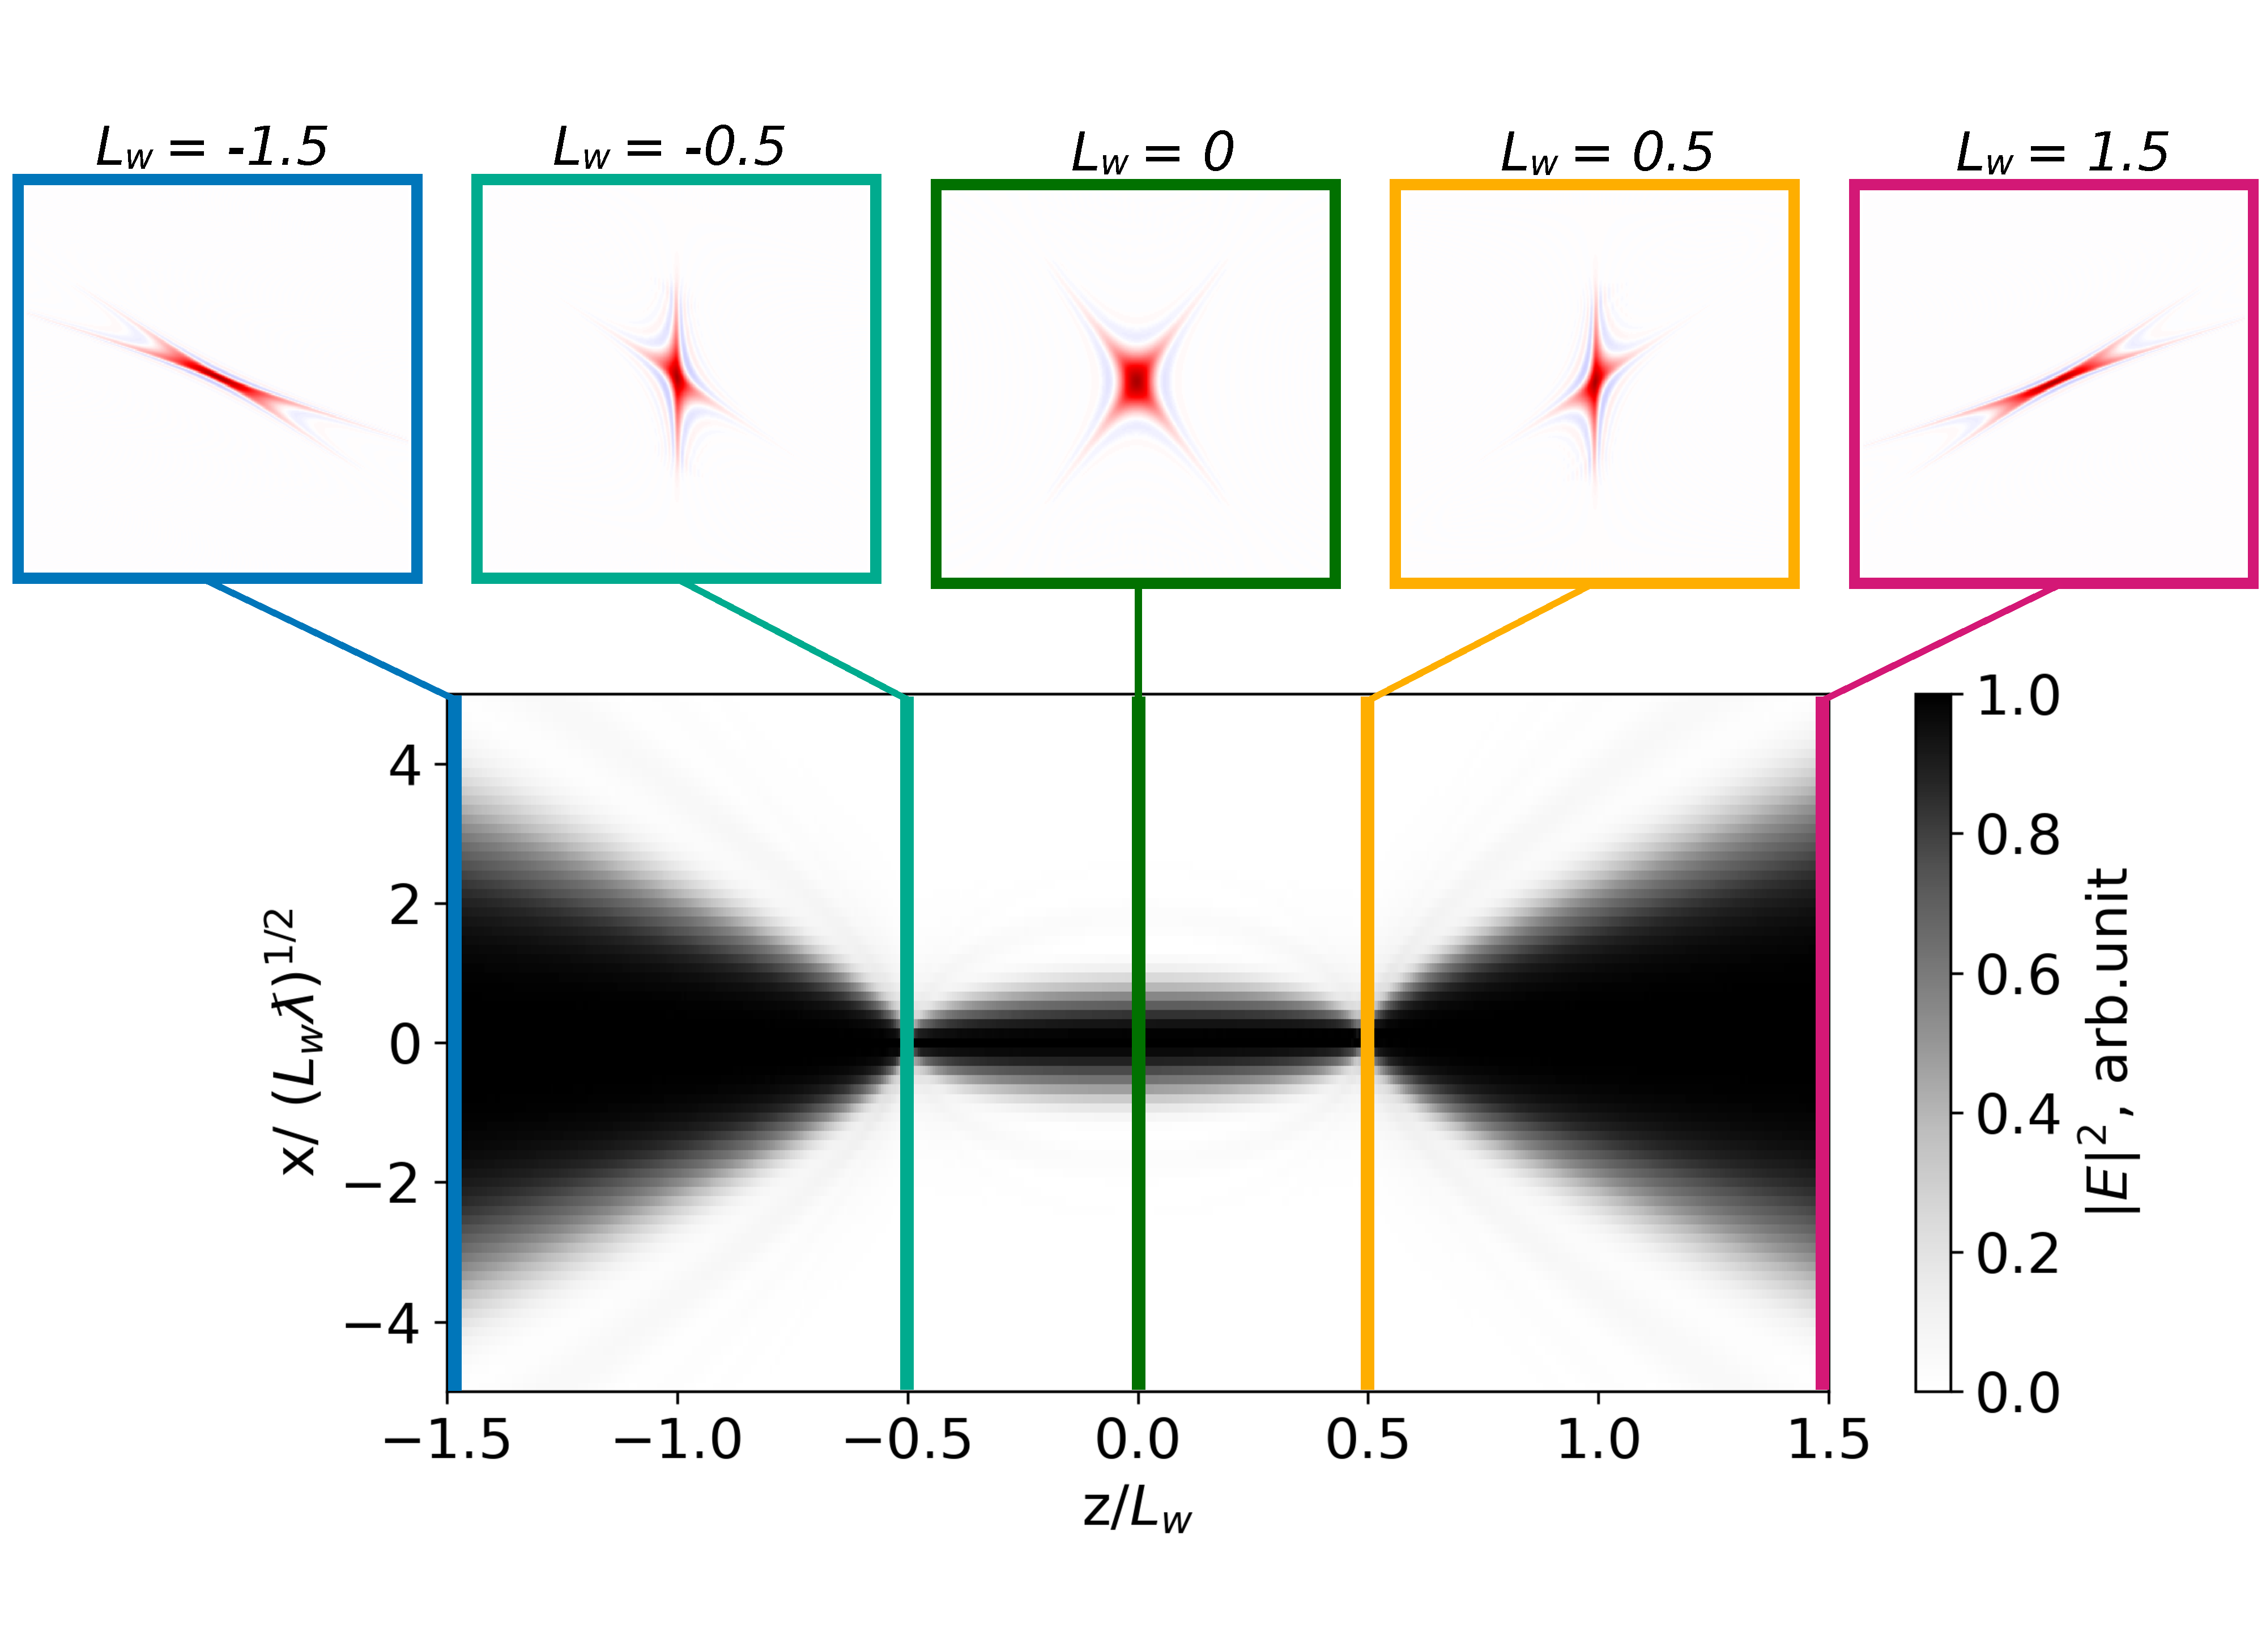
\includegraphics[width=0.9\linewidth]{content/images/Synchrotron_Radiation/Lw2_wig.pdf}
        \captionsetup{justification=centering}
        \caption{Source intensity distribution along an undulator versus the x-transverse dimension. Both axes are normalized to the natural dimensions of the system: undulator length and undulator radiation diffraction size. The intensity value along the slice over the vertical axis is normalized by the maximum of its intensity. At the top of the plot, I present Wigner function distributions at different positions along the device.}
        \label{Fig:Lw2_wig}
    \end{figure*}
    \begin{figure*}[h!]
        \centering
        \begin{minipage}{0.48\linewidth}  % Adjust width to fit within page
            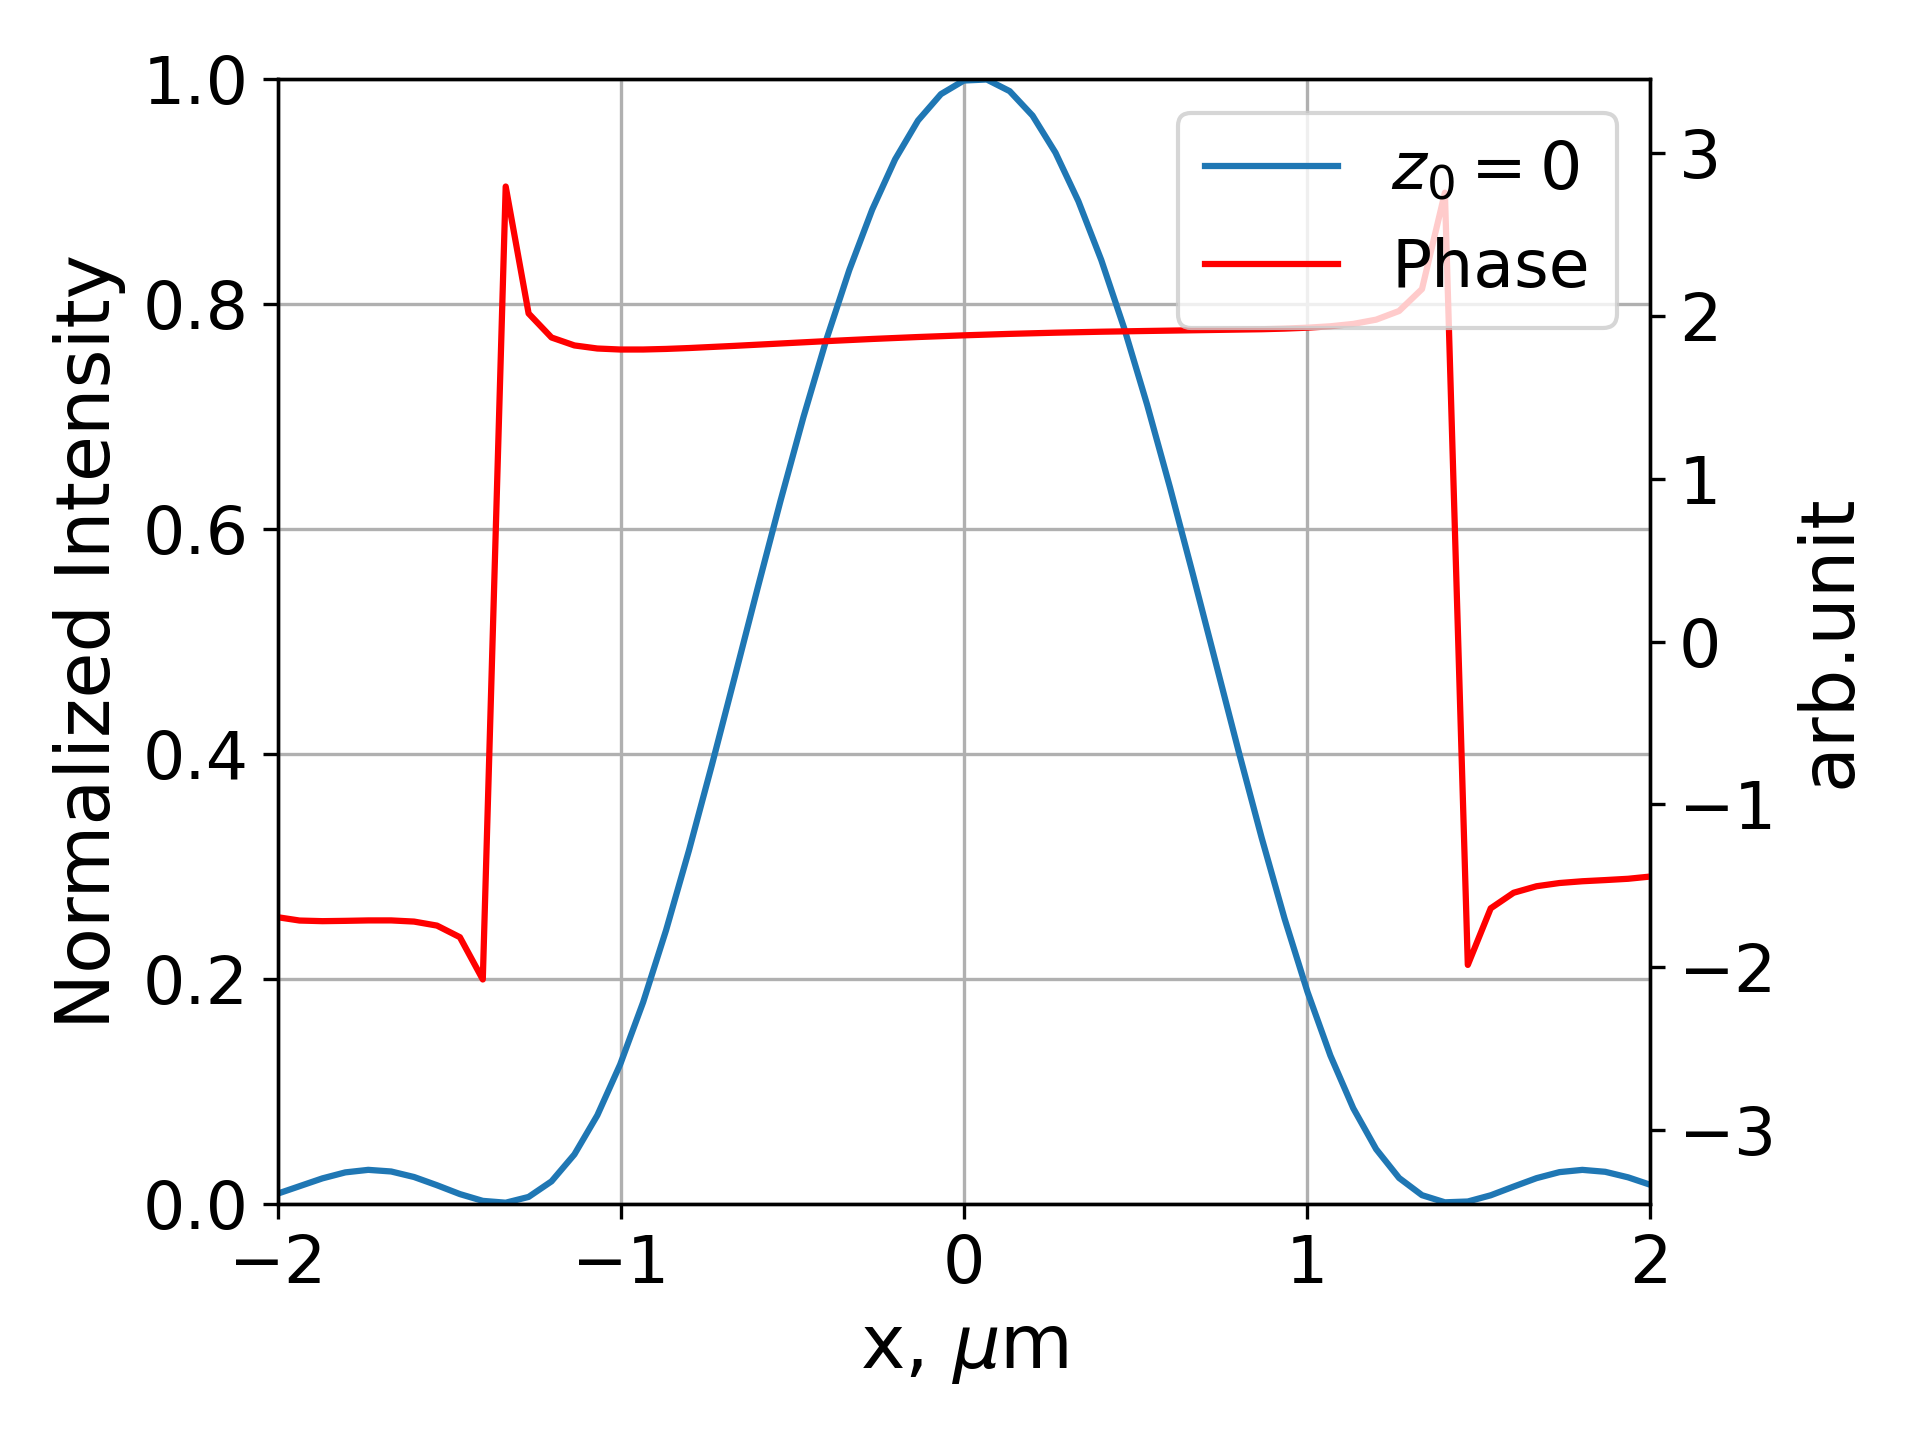
\includegraphics[width=\linewidth]{content/images/Synchrotron_Radiation/intensity_scan_N_w_100_phase_study_cross_middle.png}
            \captionsetup{justification=centering}
            \caption{Imaginary source distribution in the middle of the undulator at resonance.}  % Add your caption here
            \label{Fig:middle_scan}  % Unique label for referencing
        \end{minipage}
        \hfill  % Adds horizontal space between the figures
        \begin{minipage}{0.48\linewidth}
            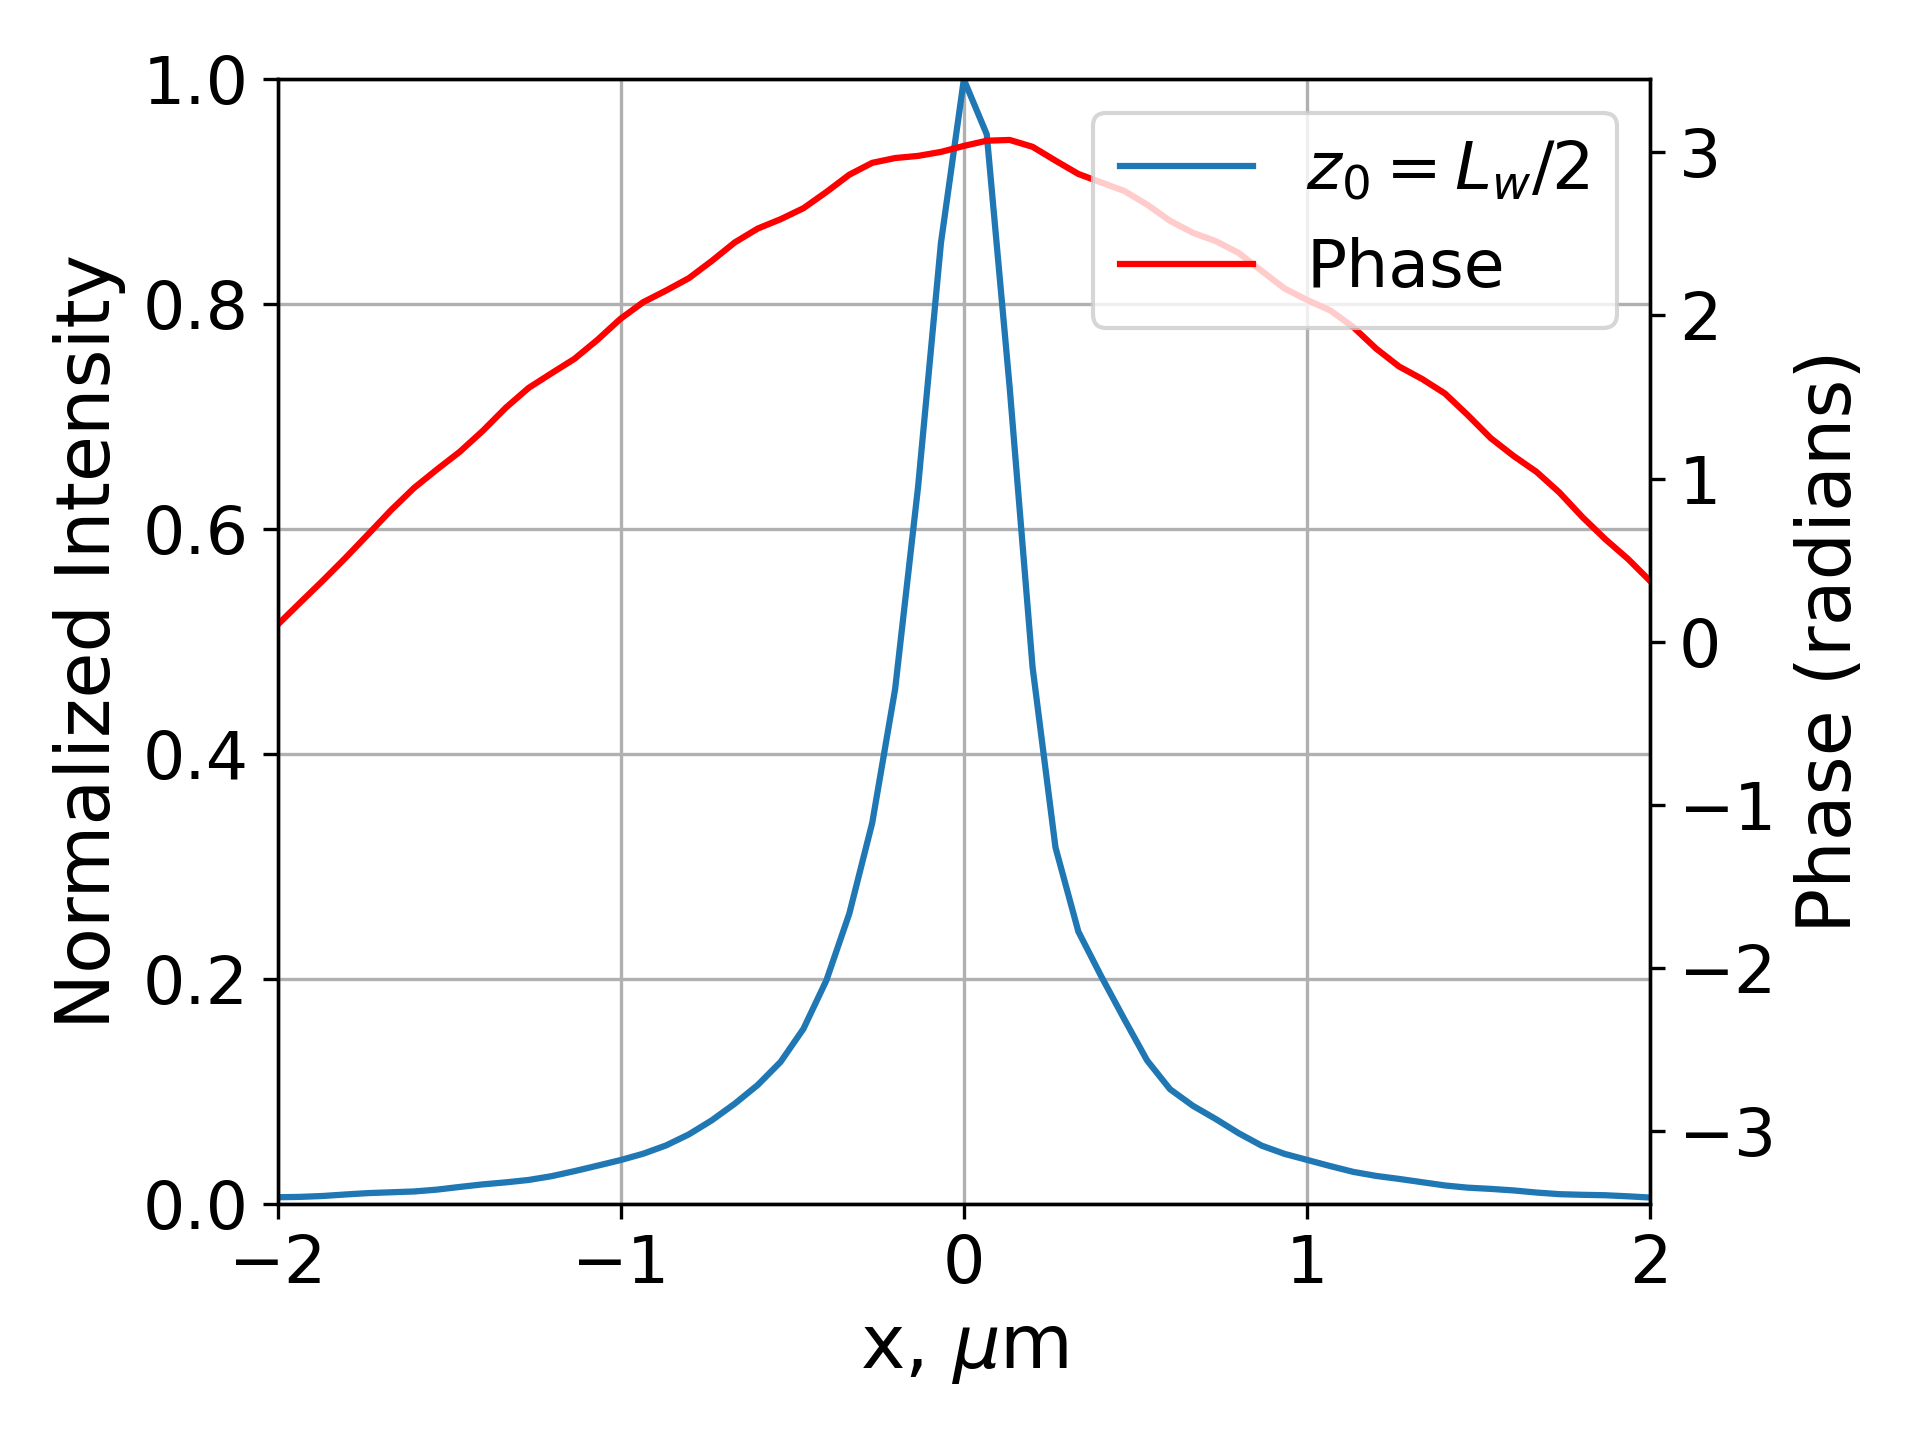
\includegraphics[width=\linewidth]{content/images/Synchrotron_Radiation/intensity_scan_N_w_100_phase_study_cross_end.png}
            \captionsetup{justification=centering}
            \caption{Imaginary source distribution at the edge of the undulator at resonance.}  % Add your caption here
            \label{Fig:end_scan}  % Unique label for referencing
        \end{minipage}
    \end{figure*}        

    Upon free-space propagation, the Wigner function distribution stretches accordingly~\cite{bazarov_synchrotron_2012}, resulting in the types of distributions depicted in the upper subplots of Fig.\ref{Fig:Lw2_wig} at both ends of the undulator. It can be observed that one axis of the "cross" is now oriented parallel to the inverse space axis. A detailed calculation of the spatial distribution reveals that there is no singularity, but the distribution is noticeably narrower compared to the center of the device. For a comparison, see Fig.\ref{Fig:end_scan} and Fig.~\ref{Fig:middle_scan}.
    
    From a mathematical perspective, the singularity arises from the combined application of the resonance approximation and the paraxial approximation, neglecting higher-order contributions in the integrand expansion, as presented in~\cite{geloni_paraxial_2005}. The authors of~\cite{geloni_fourier_2007} note that the far-field distribution and the distribution at the source are related via a Fourier transform (apart from the phase factor), implying that small features at the source correspond to large features in the far zone (and vice versa). However, the resonance and paraxial approximations restrict us to angles in the far zone that are comparable to the size of the central cone of the undulator radiation. For large angles, these approximations fail, and thus, the singularity is not truly singular but has a finite width.
    
    The reasoning presented above provides only a qualitative understanding of the nature of this feature. A reasonable question may be: what would be the size of the radiation observed in Fig.~\ref{Fig:end_scan} in terms of source parameters? Here I mean the following: the undulator radiation diffraction size is $\sqrt{L_w \lambdabar}$, which is related to the physical length of the undulator. This is precisely a resonance effect when all periods contribute to the radiation formation constructively. However, there is another typical scale in the undulator: its period length $\lambda_w$ and a diffraction size associated with $\sqrt{\lambda_w \lambdabar}$, which should also be present in the structure of the undulator radiation. From this point on, I will refer to the diffraction size related to the overall length of the undulator as the resonance one, and the one related to the undulator's period as the non-resonance one.
    
\subsection{Undulator source wiggling or out of resonance source distribution}

    To observe the non-resonant diffraction size of undulator radiation, two methods can be employed: decreasing the number of undulator periods or observing the radiation out of resonance. The first approach mitigates the resonance effect of the device. The flux density intensity scales proportionally to the square of the number of undulator periods. Thus, by reducing the number of undulator periods, one can observe more intrinsic details of the radiation at the source, which are not obscured by the resonance diffraction size. The second approach, observing radiation out of resonance, removes any resonance effects, allowing for the observation of the pure non-resonant diffraction size. I expect this size to significantly differ from the well-known resonant diffraction size: $\sqrt{L_w \lambdabar}$.
    
    If I attempt to show it mathematically I start with the far zone expression of the electric field. Modifying Eq.~\ref{Eq:funal_Eq_for_SR}: expanding $1/(z_0 - z')$ around $z_0$ and using $\vec{\theta} = (\vec{r}_{\perp_0} - \vec{r}'_{\perp}) / (z_0 - z')$ I write:
    \begin{align}
        \vec{\tilde{E}}(\vec{\theta}, z_0, \omega) = -\frac{i \omega e}{c^2 z_0} \int_{-\infty}^{\infty} dz' \left( \frac{\vec{v}(z')}{c} - \vec{\theta} \right) \exp\left( i \omega \left[ \frac{s(z')}{v} - \frac{z'}{c} \right] + \frac{i \omega}{2 c} \left[ z_0 \theta^2 - 2 \vec{\theta} \cdot \vec{r}'(z') + z' \theta^2 \right] \right)
        \label{Eq:far_zone_field_wiggling_feature}
    \end{align}
    I can obtain the virtual source field at the position $z = z_s$ from Eq.~\ref{Eq:far_zone_field_wiggling_feature} by back propagating this field to the source location using the expression from~\cite{geloni_fourier_2007}:
    \begin{align}
        \vec{\tilde{E}}(\vec{r}, z_s, \omega) = \cfrac{i \omega z_0}{ 2 \pi c}\int_{-\infty}^{\infty} d\vec{\theta} \exp{\bigg[-\cfrac{i \omega \theta^2}{2 c} (z_0 + z_s) \bigg]} \vec{\tilde{E}}(\vec{\theta}, z_0, \omega) \exp{\bigg[\cfrac{i \omega}{c}\vec{r}\cdot\vec{\theta} \bigg]}.
    \end{align}
    and substituting Eq.~\ref{Eq:far_zone_field_wiggling_feature} in this I obtain:
    \begin{align}
        \vec{\tilde{E}}(\vec{r}, z_s, \omega) = \cfrac{\omega^2 e}{2 \pi c^3} \int_{-\infty}^{\infty} dz' \int_{-\infty}^{\infty} d\vec{\theta} \left( \frac{\vec{v}(z')}{c} - \vec{\theta} \right) \exp\left( i \omega \left[ \frac{s(z')}{v} - \frac{z'}{c} \right]\right) \cr \exp\left(\frac{i \omega}{2 c} \left[(z' - z_s)\theta^2 + 2\vec{\theta}\cdot (\vec{r} - \vec{r}'(z')) \right] \right).
    \end{align}   
    The first exponent is oscillatory at scales larger than the formation length $L_f$ as one integrates along $z'$. Consequently, the integral limits can be set to $(-L_f, L_f)$ at most. This simplification remains general and does not depend on the type of source considered. The value of $L_f$ can vary significantly depending on the chosen magnetic configuration. For undulator radiation, I seek evidence that the diffraction size differs from the resonant one determined by the length of the undulator $L_w$.

    The second exponent contains a phase that is also oscillatory as one integrates over $\vec{\theta}$. Intuitively, within the range of $z_s$ around the "virtual source" ($-L_f, L_f$), the integral is significant for $\vec{r} \approx \vec{r}'(z_s)$. According to the energy conservation law, all energy in the pulse will be concentrated around this location at the source.
    
    Thus, I estimate the integration range for angles to be $\theta_{x, y} < \sqrt{2c/(\omega (z' - z_s))}$, assuming $z'$ varies only slightly within ($-L_f, L_f$). We observe large field values only within ($-L_f, L_f$) since the field diverges further from the source. Therefore, at most $|z' - z_s| \sim L_f$, giving the estimation $\theta_{x, y} < \sqrt{2c/(\omega L_f)}$. Finally, the last term remains small only for deviations of $\vec{r}$ from the trajectory up to the order of $\delta r \sim c / \omega \sqrt{\omega L_f / c} \sim \sqrt{(cL_f)/\omega}$, which is the typical diffraction size.

    At this point, I have determined that the diffraction size of the radiation is $\delta r \sim \sqrt{(cL_f)/\omega}$, as expected. It does not contradicts the hypothesis that there are two typical scales: one related to the undulator length and the other to its period length. The former is usually associated with undulators, where the diffraction size is considered to be $\sqrt{(cL_w)/\omega}$. However, the presence of the second natural scale suggests that there should be a smaller diffraction size related to the device period $\lambda_w$, thus the diffraction size can be written as $\sqrt{(c\lambda_w)/\omega}$. 
    
    To confirm this hypothesis, I shall break the resonance approximation typically used in analytical calculations and decrease the number of undulator periods. This results in a specific "wiggling" of the undulator source, as illustrated in Figs.~\ref{Fig:intensity20}, \ref{Fig:intensity10}, \ref{Fig:intensity5}. 
    \begin{figure*}[p] 
        \centering
        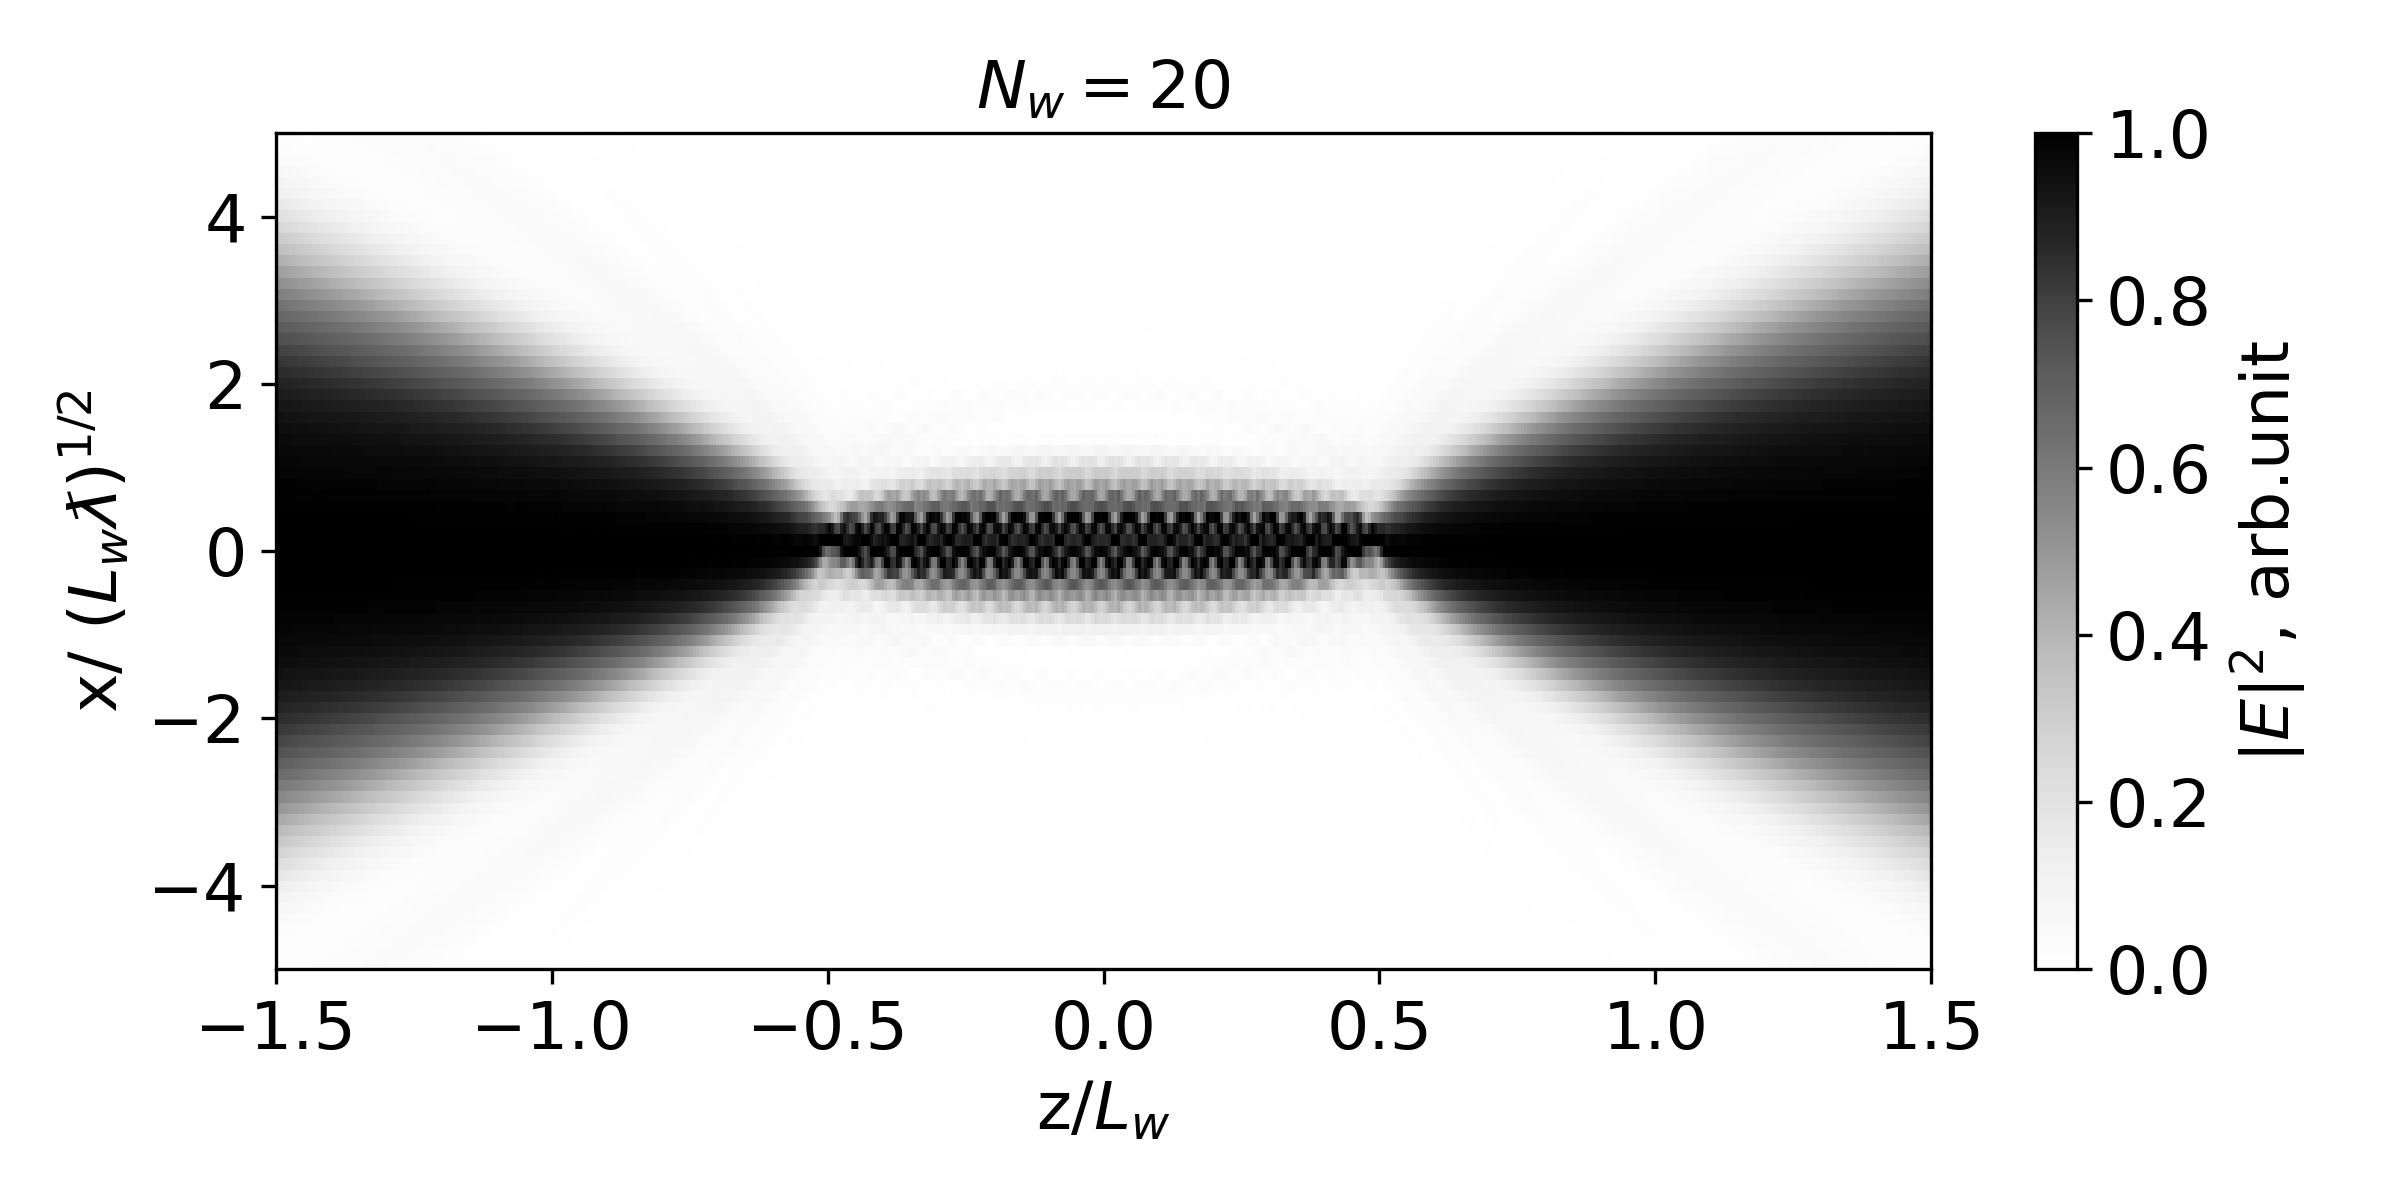
\includegraphics[width=0.9\linewidth]{content/images/Synchrotron_Radiation/intensity_scan_N_w_20.png}
        \captionsetup{justification=centering}
        \caption{}
        \label{Fig:intensity20}
        
        \vspace{\floatsep} % Adds some space between the figures
        
        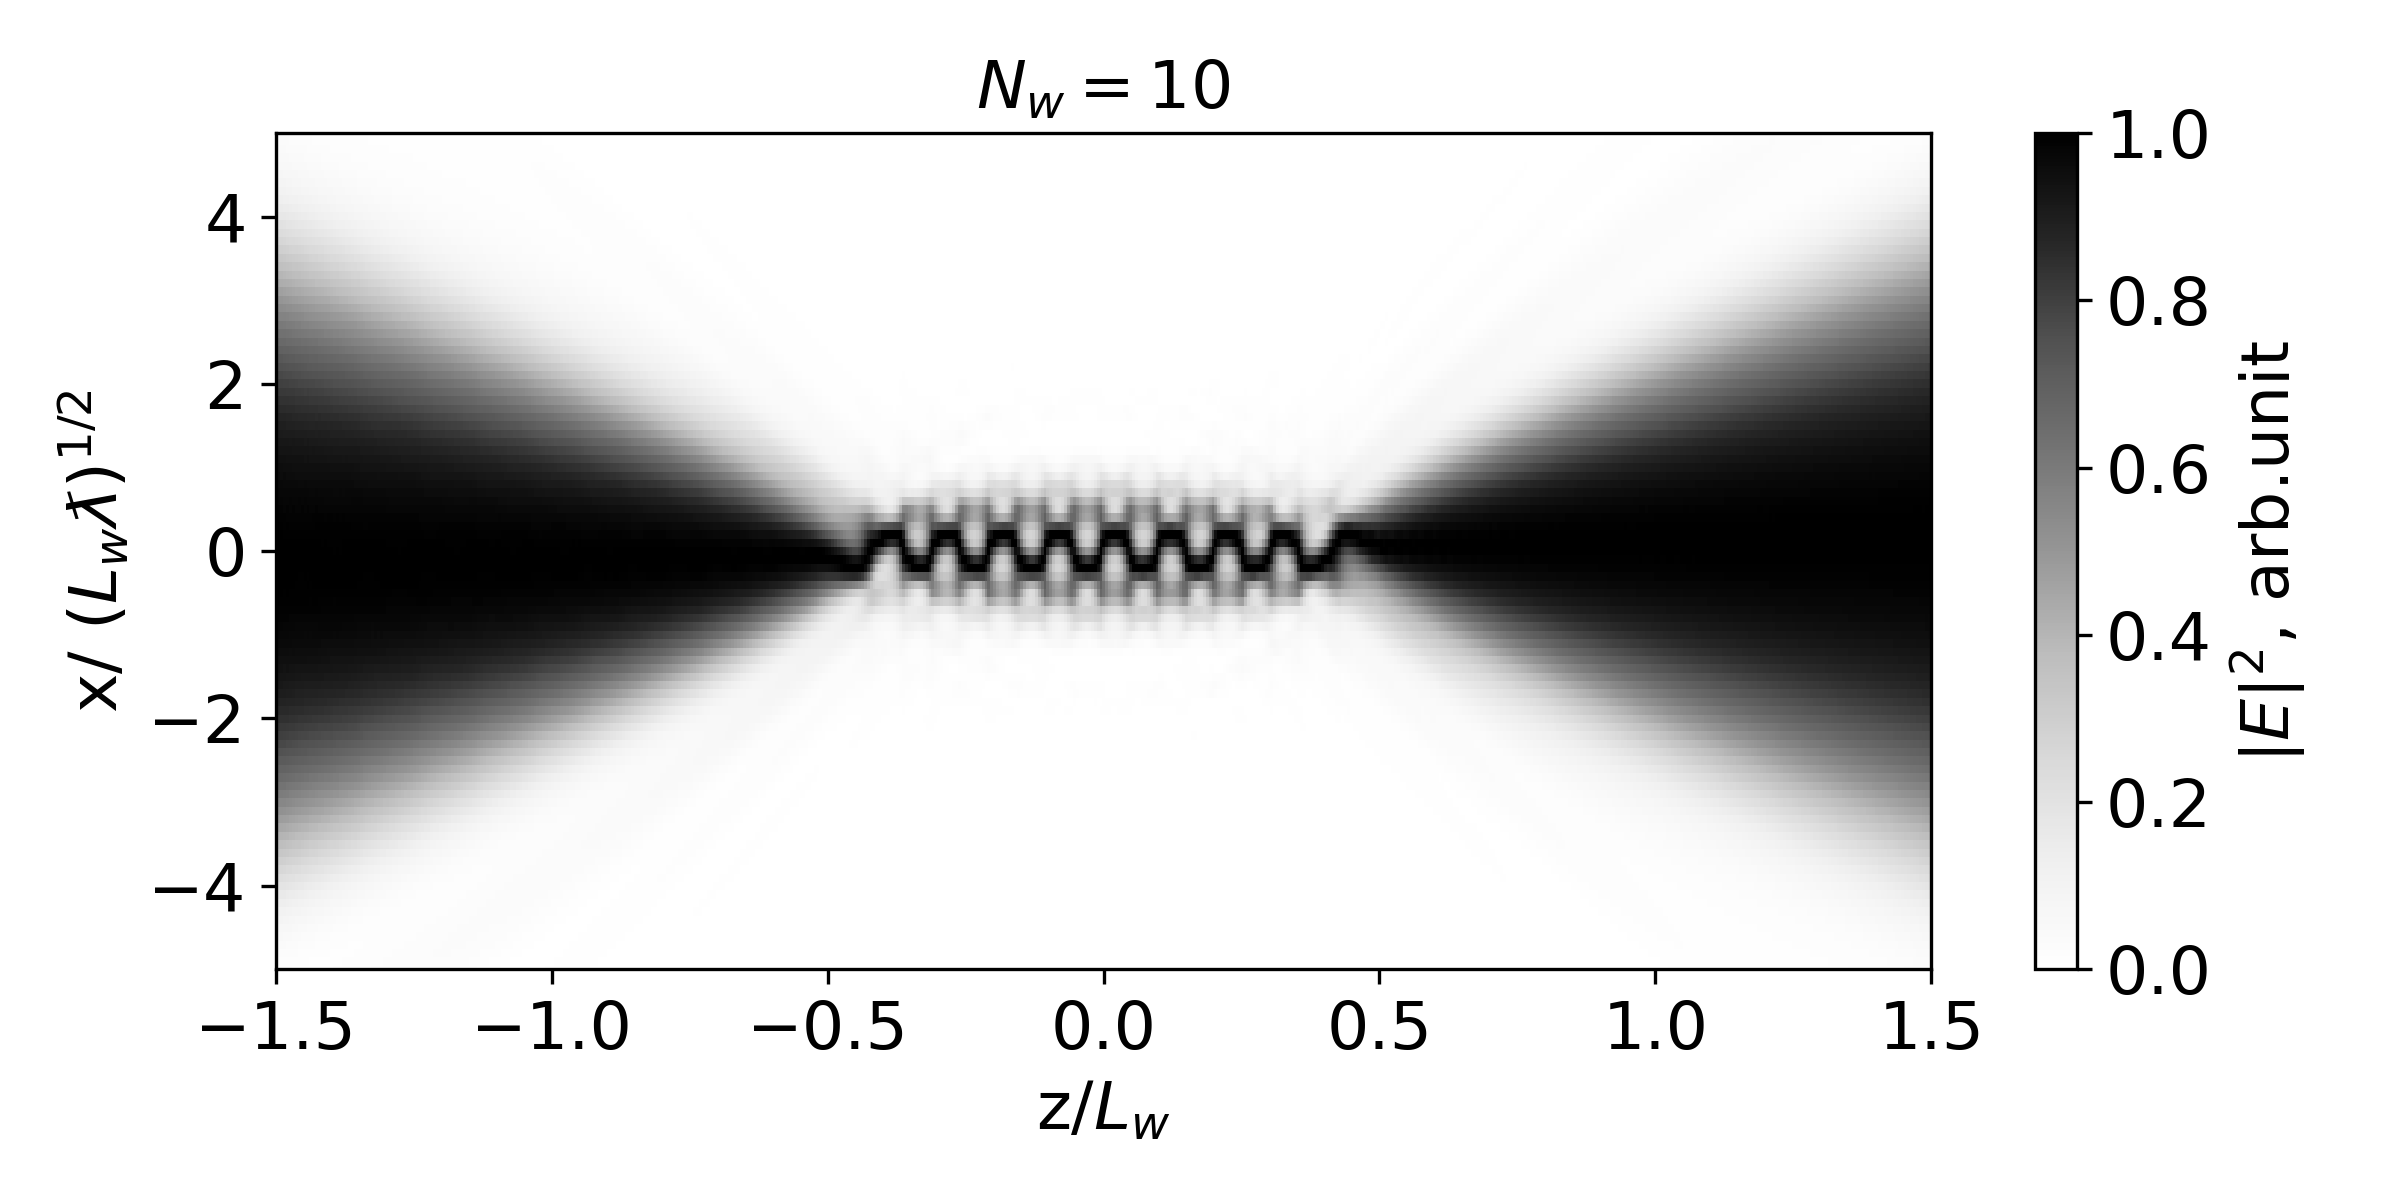
\includegraphics[width=0.9\linewidth]{content/images/Synchrotron_Radiation/intensity_scan_N_w_10.png}
        \captionsetup{justification=centering}
        \caption{}
        \label{Fig:intensity10}
        
        \vspace{\floatsep} % Adds some space between the figures
        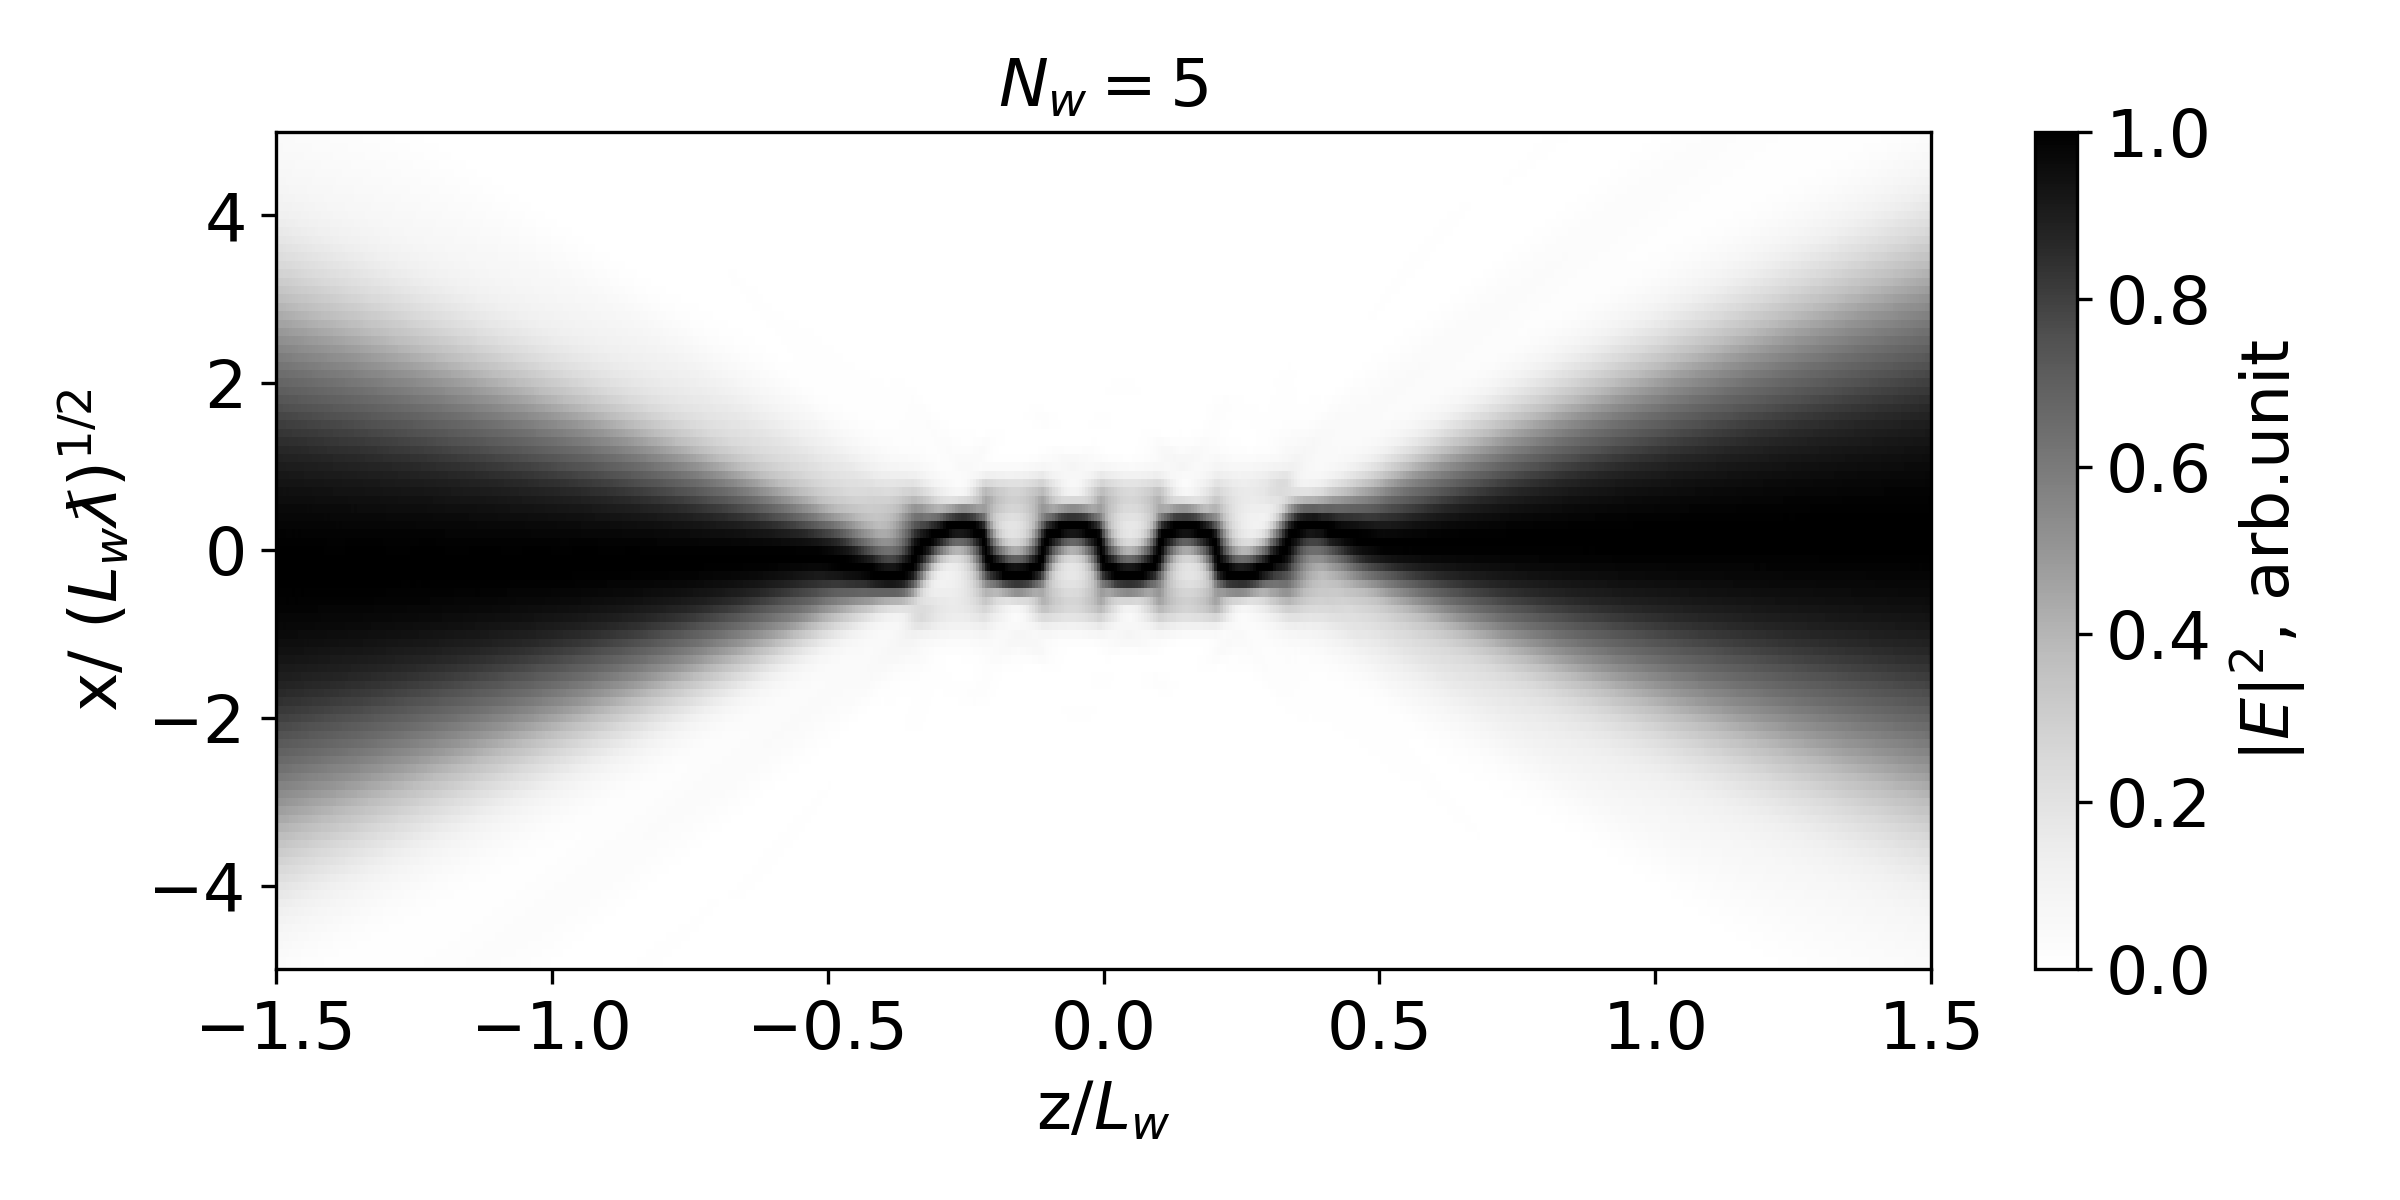
\includegraphics[width=0.9\linewidth]{content/images/Synchrotron_Radiation/intensity_scan_N_w_5.png}
        \captionsetup{justification=centering}
        \caption{"Wiggling" of the undulator source distribution. From up to down source distributions of 20 periods, 10 period, and 5 period devices.}
        \label{Fig:intensity5}
    \end{figure*}
    As one can see, I observe a finer, non-resonant structure of the undulator radiation superposed with the resonant one. 

    To clearly observe this effect, I examine the out-of-resonance case of the same radiation from a ten-period device. One can observe the "pure" wiggling of the source as depicted in Fig.~\ref{Fig:intensity_scan_N_w_10_out_of_resonance}, and intensity slices over specific locations are shown in Fig.~\ref{Fig:intensity_scan_N_w_10_out_of_resonance_slices}.

    \begin{figure*}[h!]
        \centering
        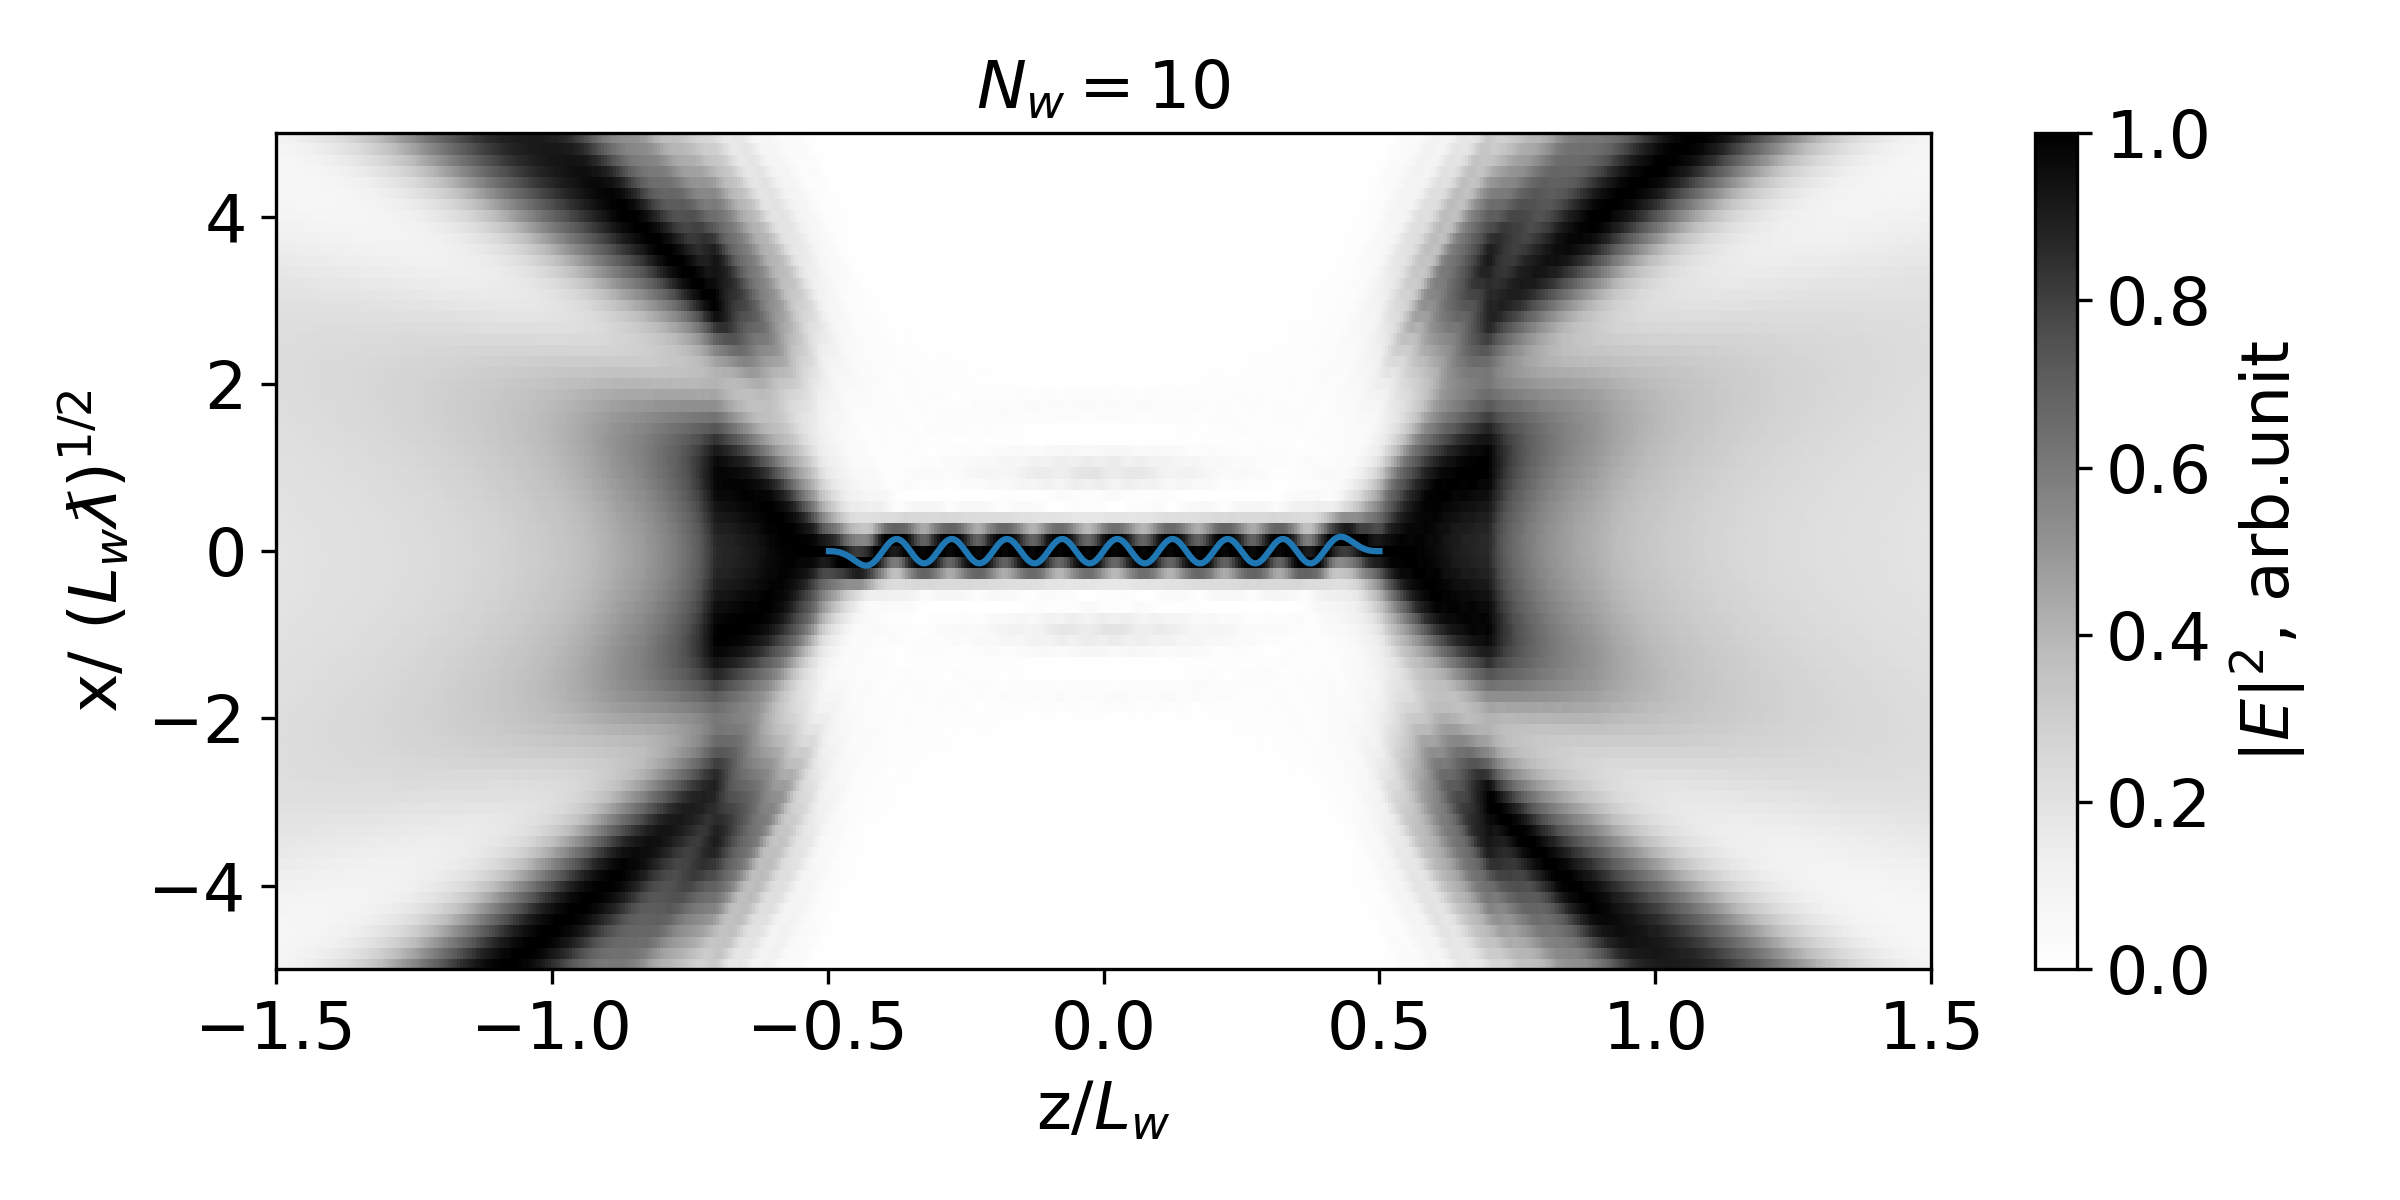
\includegraphics[width=0.9\linewidth]{content/images/Synchrotron_Radiation/intensity_scan_N_w_10_out_of_resonance.png}
        \captionsetup{justification=centering}
        \caption{"Wiggling" of the undulator source distribution for the out-of-resonance case, with the frequency set between the 1st and 2nd harmonics.}
        \label{Fig:intensity_scan_N_w_10_out_of_resonance}
    \end{figure*}

    \begin{figure*}[h!]
        \centering
        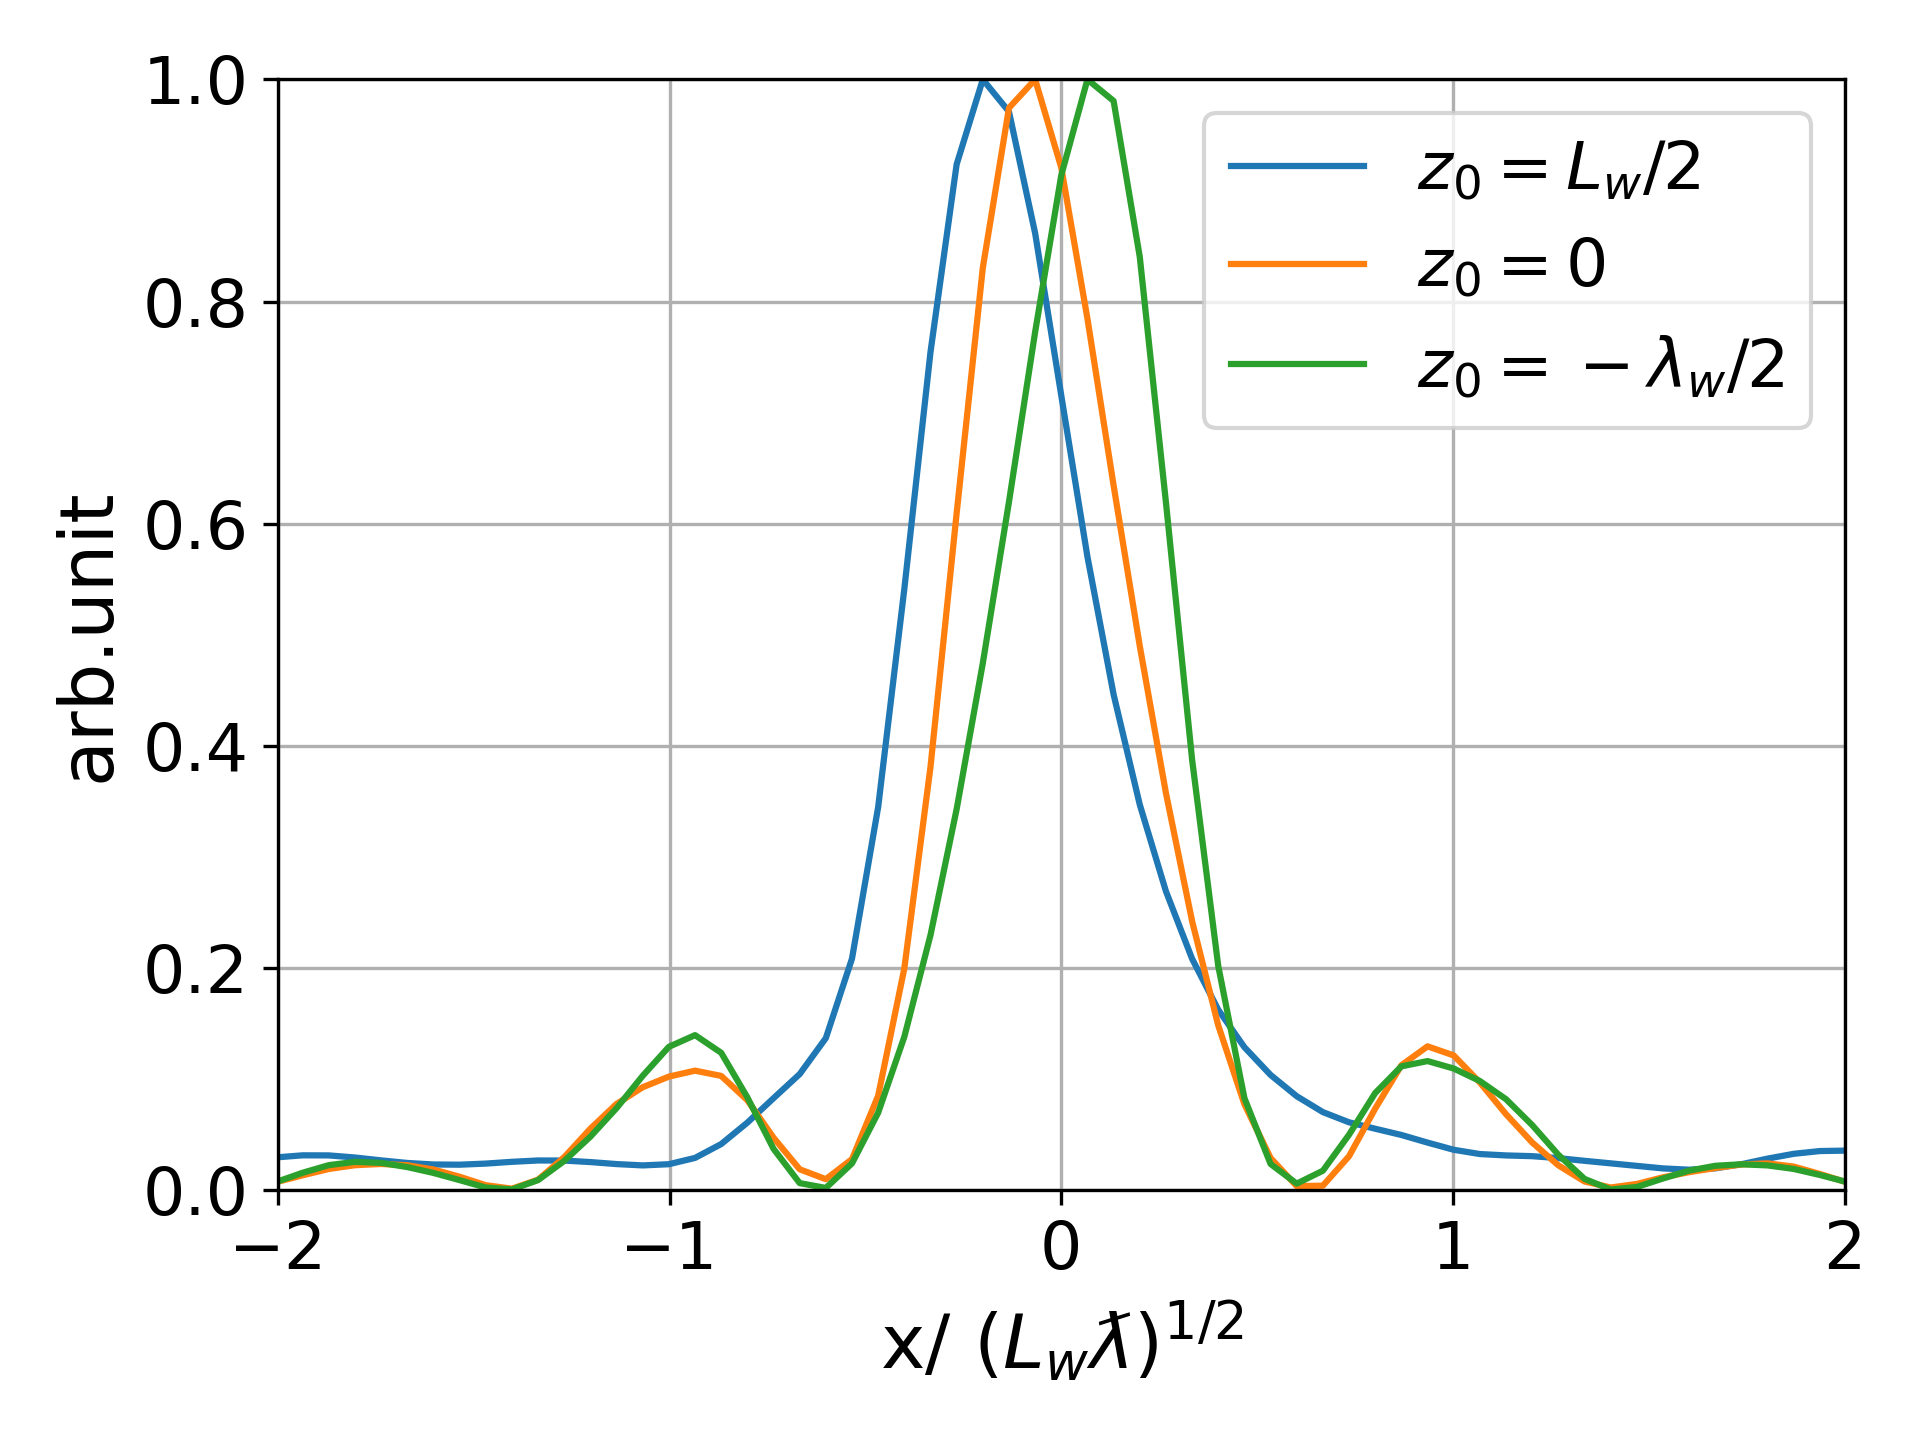
\includegraphics[width=0.5\linewidth]{content/images/Synchrotron_Radiation/intensity_scan_N_w_10_out_of_resonance_slices.png}
        \captionsetup{justification=centering}
        \caption{"Wiggling" of the undulator source distribution for the out-of-resonance case shown for the intensity slices.}
        \label{Fig:intensity_scan_N_w_10_out_of_resonance_slices}
    \end{figure*}
    The most straightforward measurements needed to reveal the non-resonant diffraction size of undulator radiation are coherence measurements of the out-of-resonance undulator radiation. This method reveals the coherence area, the size of which is related to the single-electron radiation diffraction size. In this case, one would expect to detect a significantly smaller coherence area compared to the in-resonance case at the same wavelength. These measurements do not require special conditions, but an interferometers should be placed off the optical axis because the radiation will be observed out of resonance. 
    
    \rr{add citation on possible kinds of interferometers}
    
    The second type of measurement can be direct imaging of the radiation source, provided the emittance of the electron beam is much smaller than the diffraction size of radiation from a single electron. This can be achieved either by using an imaging system with a point spread function much smaller than the single-electron diffraction size or by measuring the wavefront distribution directly \rr{cite} and then using back-propagation methods to trace the radiation back to the source analytically.
    
    \rr{probably, one needs the drawn schemes…}
    
\subsection{Brightness of undulator radiation}
    It is also valuable to examine the brightness of undulator radiation at the source location, defined as the maximum of the Wigner function distribution. This can be achieved by scanning the positions along the undulator and as a function of the detuning parameter $C$ from the resonance, as shown in Fig.~\ref{Fig:badman}.
    \begin{figure*}[h!]
        \centering
        \begin{minipage}[b]{0.48\linewidth}
            \centering
            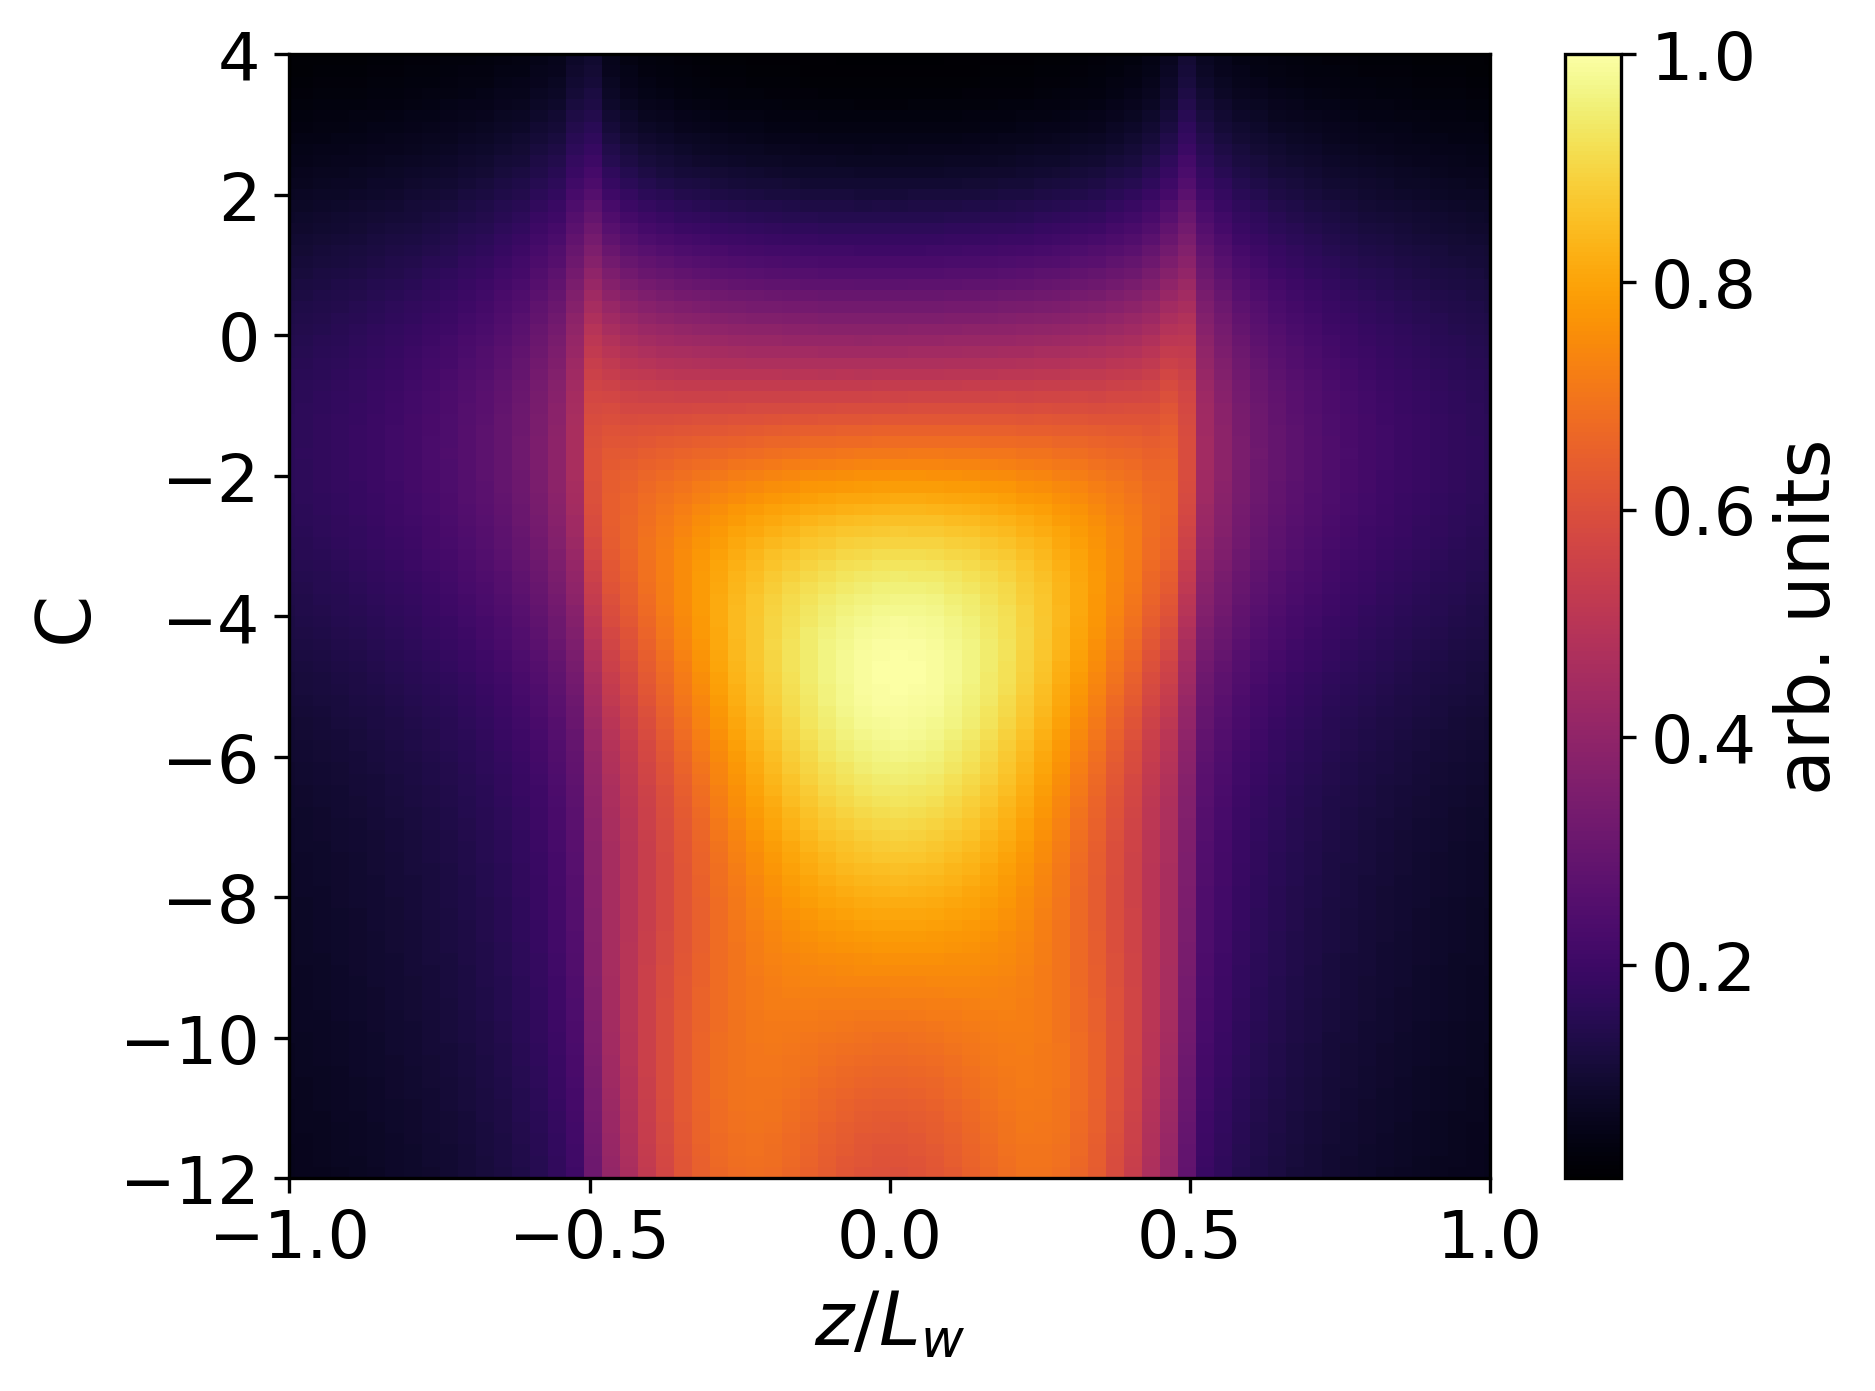
\includegraphics[width=\linewidth]{content/images/Synchrotron_Radiation/badman.png}
            \captionsetup{justification=centering}
            \caption{}
            \label{Fig:badman}
        \end{minipage}
        \hspace{0.02\linewidth}
        \begin{minipage}[b]{0.48\linewidth}
            \centering
            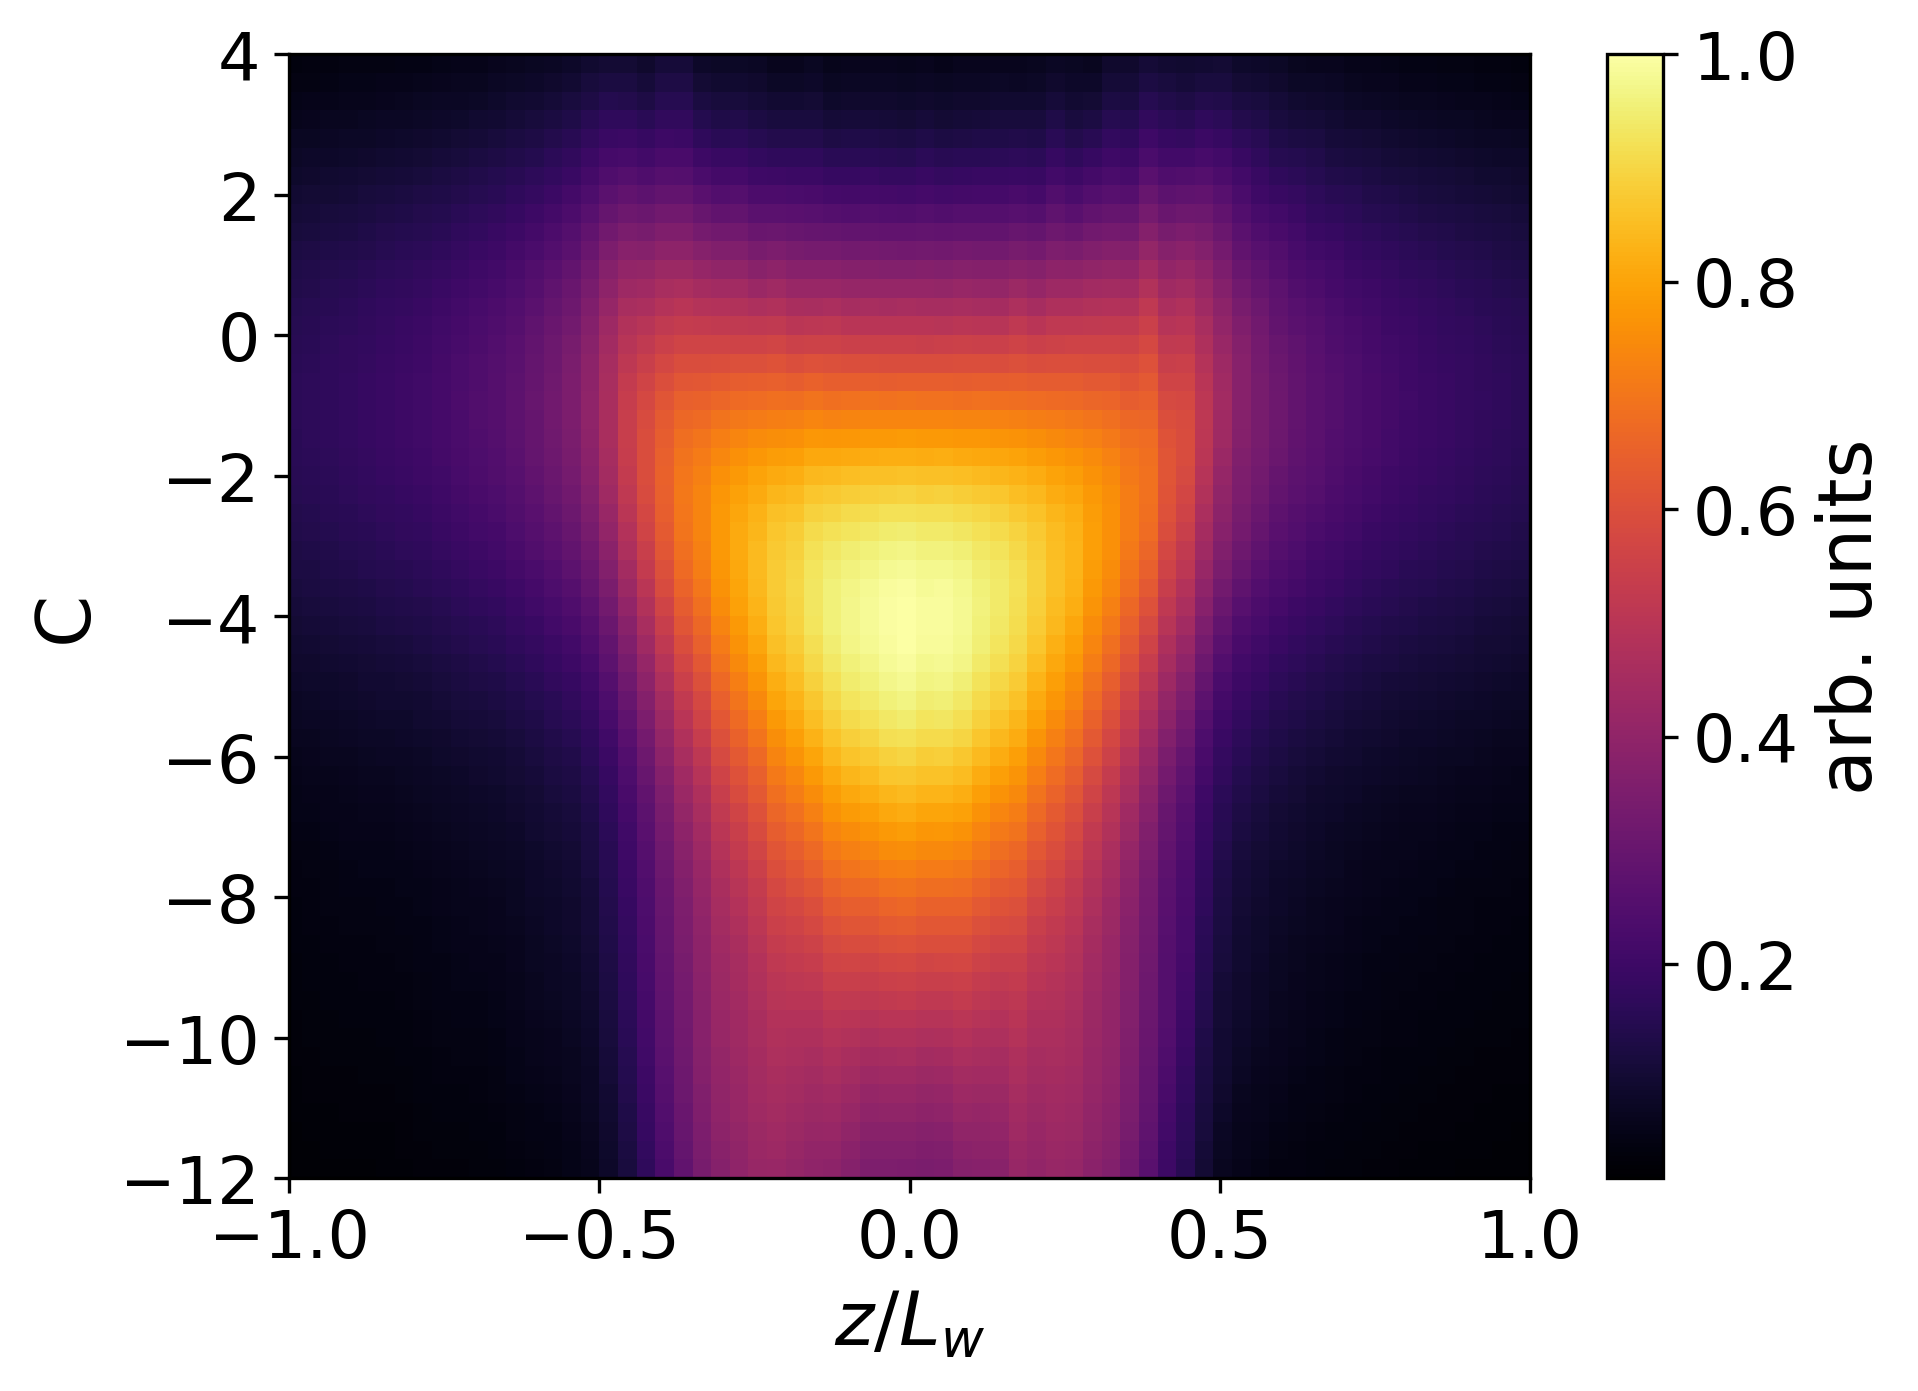
\includegraphics[width=\linewidth]{content/images/Synchrotron_Radiation/badman_Nw_10.png}
            \captionsetup{justification=centering}
            \caption{}
            \label{fig:badman_Nw_10}
        \end{minipage}
        \caption{"Badman" diagram. Horizontal axis corresponds to the position along the undulator and the vertical axis reflects the detuning parameter $C$.}
    \end{figure*}
    Apart from the global maximum around $C = -4$ and $z = 0$, the maxima for the perfectly in-resonance case ($C = 0$) are not located in the middle of the undulator but at either end of the device.

    In conclusion, this effect needs to be studied in more detail both analytically and experimentally. However, an analytical treatment of the problem is complicated when considering undulator radiation not applying the resonance approximation. From the experimental point of view, the measurements does not require subtle setups and can be conducted using the available hardware of modern SR source optical systems only with slight modifications.
\chapter{Gaussian random field generators for simulating partially coherent radiation}
\label{Chapter:Gaussian random field generators for simulating partially coherent radiation}
%\label{Chapter:White noise based algorithms for modeling Gaussian random processes}

    \rr{Say more about advantages and disadvantages of SERVAL to better show the difference between the common methods and SERVAL}  

    Radiation sources typically comprise numerous emitters contributing to the emission process. As the number of emitters becomes exceedingly large, it becomes impractical to describe these sources deterministically, leading to their characterization as random sources. In such scenarios, the theory of statistical optics offers an ideal framework for describing the behavior of electromagnetic fields emitted by these sources. Examples of random sources include thermal sources like stars and light bulbs, as well as radiation from ultra-relativistic particle bunches, such as synchrotron radiation and self-amplified spontaneous emission (SASE) free-electron laser (FEL) radiation in the linear regime. A common feature among these sources is their adherence to Gaussian statistics. According to the central limit theorem, as the number of random emitters increases, the resulting radiation, regardless of the probabilistic laws governing individual emitters, tends to follow a Gaussian statistics.

    \rr{finalise this…}  
    There are several methods for simulating statistical optics phenomena and the most frequently applied in the synchrotron radiation and FEL communities are mode decomposition methods~\rr{cite} and Monte-Carlo-based simulations, where radiation from each particle is simulated separately~\cite{chubar_accurate_1998, reiche_genesis_1999}. … 

    In this chapter, I present a set of methods for simulating Gaussian random fields based on a computationally efficient algorithm that leverages the properties of Gaussian random noise. This algorithm shapes the field distribution by multiplying the noise distribution with specifically chosen mathematical supports. These methods are designed exclusively for Gaussian random fields. However, there is potential to extend these methods to non-Gaussian statistics, as demonstrated in~\cite{hong_algorithm_2021}. Although these algorithms were developed for simulating synchrotron radiation (SR) sources and self-amplified spontaneous emission (SASE) free-electron laser (FEL) radiation, they can be easily extended to all optical fields that are stochastic and follow Gaussian statistics.
   
    These methods necessitate an introduction to the fundamentals of statistical optics theory, which I present earlier in this chapter. I begin with general definitions of random processes and their properties. Delving into the concepts of stationarity and ergodicity, I discuss differences in averaging processes: over time versus across different statistical realizations. Then, I introduce the central theoretical concept for this thesis—Gaussian random processes. Subsequently, I present the theory for quasi-stationary sources in a manner similar to that used in~\cite{mandel_optical_1995, goodman_statistical_2015} for stationary sources. I provide a proof of a generalized form of the Wiener-Khinchin theorem. This generalization accounts for the quasi-stationarity of a source and relates the finite duration of the pulse to spectral coherence properties. From the longitudinal coherence properties of radiation, I transition to the transverse domain of radiation and offer a derivation of the generalized van Cittert-Zernike theorem. Following this, I discuss the coherence properties of synchrotron and SASE FEL radiation, along with well-established methods for simulating these types of radiation sources. To this end, I introduce white-noise-based methods for simulating partially coherent radiation. Each method is first presented through heuristic considerations, which are then extended to applications in simulation problems: bending magnet radiation, undulator radiation, and FEL SASE radiation, as represented in Papers I, II, and III. Finalizing this chapter, I present an experimental method for generating sub-femtosecond level pulses at FEL facilities. The statistics of the pulses deviate from Gaussian behavior. This result showcases that the proposed algorithms should be applied carefully to the studied case when attempting to replicate the results in simulations.

\section{Classification of random processes}

    \rr{Say that the narrative here is shorten to the bare minimum needed for this thesis, and surely one can find more detail in~\cite{mandel_optical_1995, goodman_statistical_2015}. Also it should be noted separately, that I introduce theory for quasi-stationary sources, which is not presented in the textbooks}
    
    In this section, I will introduce the basic notations and concepts of statistical optics. I primarily follow the textbooks~\cite{mandel_optical_1995, goodman_statistical_2015} with slight modifications to encompass quasi-stationary sources in the theory. I start by introducing a random process $U$. This process consists of statistical realizations, which I denote as $u^{[k]}$. Unlike a random variable, such as a single roll of a dice, a random process also depends on time, represented as $u^{[k]}(t)$. Realistically, an observer can observe this process over a finite time interval $[-T/2, T/2]$. The process is random, meaning that the exact value of a given statistical realization $u^{[k]}(t_0)$ at a specific moment in time $t_0$ cannot be predicted in advance. One objective way to make predictions about a statistical process is to define statistical moments, which can be defined as follows:
    \begin{align}
        \overline{u(t)} = \frac{1}{T} \int \limits_{t - T/2}^{t + T/2}  u^{[k]}(t') dt',
        \label{Eq:time_avr}
    \end{align}
    and for the second moment or \textit{time auto-correlation function} I write:
    \begin{align}
        \overline{u(t_1)u(t_2)} = \frac{1}{T} \int \limits_{t - T/2}^{t + T/2} u^{[k]}(t + t_1)u^{[k]}(t + t_2)dt.
        \label{Eq:time_autocorrelation}
    \end{align}
    \rr{…and conclude…}
    
    For each process, I can define a set of probability density functions $p(u, t_i)$, which depend on both time and the chosen realization. To fully describe a statistical process, one needs to know not only $p(u, t_i)$—the first-order probability density function—but also its higher-order counterparts that contain information about correlations at different moments in time: $t_1, t_2, \ldots, t_n$, where, in principle, $n$ should be infinite. Therefore, one needs to know the second-order moment $p_2(u_1, t_1, u_2, t_2)$, the third, and up to the $n$-th order joint probability density function $p_n(u_1, t_1, u_2, t_2, \ldots, u_n, t_n)$. \rr{…again need to be concluded…} To anticipate, in the next chapter, I will introduce a type of process called Gaussian, where the process can be fully defined only by knowing the first and second-order probability density functions. With probability density functions I can define the ensemble averaging operation:
    \begin{align}
        \langle u(t) \rangle = \int u p(u, t) du,
        \label{Eq:ensemble_int_avr}
    \end{align}
    and similarly for the second order:
    \begin{align}
        \Gamma(t_1, t_2) = \langle u(t_1)u(t_2) \rangle = \iint u_1u_2 p_2(u_1, t_1, u_2, t_2) du_1du_2,
        \label{Eq:ensemble_int_autocorrelation}
    \end{align}
    and so on for higher order correlation functions. In principle, to fully describe a process, one needs to know all higher-order auto-correlation functions. However, in practice, it is often not possible to know all joint probability functions. In this case, one can utilize another useful definition of the ensemble averaging. If one collects a reasonably large statistical ensemble: $u^{[1]}(t), u^{[2]}(t), \ldots, u^{[k]}(t)$, then the ensemble average can be defined as averaging over the realisations:
    \begin{align}
        \langle u(t) \rangle = \lim_{N\to\infty} \frac{1}{N}\sum_{i=1}^{N} u^{[i]}(t)
        \label{Eq:ensemble_avr}
    \end{align}
    and the same for the second order auto-correlation function:
    \begin{align}
        \Gamma(t_1, t_2) = \langle u(t_1)u(t_2) \rangle = \lim_{N\to\infty} \frac{1}{N}\sum_{i=1}^{N} u^{[i]}(t_1)u^{[i]}(t_2),
        \label{Eq:ensemble_autocorrelation}
    \end{align}
    and so on for higher-order correlation functions. These definitions are fully equivalent to Eq.~\ref{Eq:ensemble_int_avr},~\ref{Eq:ensemble_int_autocorrelation}but are much more useful in practice. They only require measurement of the realizations themselves without any \textit{a priori} knowledge about the process. In this thesis, I will mostly rely on these latter definitions for practical calculations and the experiments.
    
    \subsection{Stationarity and ergodicity}
    
    Continuing the discussion about random processes, it is essential to identify properties that classify these processes and establish governing laws. In this subsection, I will introduce two important concepts in statistical optics: stationarity and ergodicity. These concepts classify processes based on their temporal characteristics and link these characteristics to their statistical realizations.

    I can define a requirement for a process to be stationary if all its joint probability density functions has the following property:
    \begin{align}
        p_n(u_1, t_1, u_2, t_2, …u_n, t_n) = p_n(u_1, t_1 + T, u_2, t_2 + T, …u_n, t_n + T) \; \textup{for all} \; T
        \label{Eq:stationary_strict}
    \end{align}
    As the choice of $T$ is arbitrary, we can set it to be one of the $t_n$ variables and find that, for example, the autocorrelation function depends only on the time difference $\Delta t = t_2 - t_1$.
    \begin{align}
        \Gamma(t_1, t_2) = \lim_{N\to\infty} \frac{1}{N}\sum_{i=1}^{N} u^{[i]}(t)u^{[i]}(t + t_2 - t_1) = \langle u(t)u(t + t_2 - t_1) \rangle
    \end{align}
    for all $t$ values.

    
    The definition in Eq.~\ref{Eq:stationary_strict} is also called \textit{strict-sense stationarity} because it requires that all orders of the joint probability function follow that definition. In practice, when one is interested only in the average and the first-order correlation function, a weaker definition can be used. If these two quantities are stationary, the process is called \textit{wide-sense stationarity}.

    As one can see, there are two conceptual ways to define averages in statistical optics: \textit{over} time and \textit{across} different realizations. In general, these averages should be different, but there is a specific type of process for which these two averages are equivalent. This type of process is called \textit{ergodic}. Writing the definition for this explicitly:
    \begin{align}
        \lim_{N\to\infty} \frac{1}{N}\sum_{i=1}^{N} u^{[i]}(t) = \frac{1}{T} \int \limits_{t - T/2}^{t + T/2}  u^{[k]}(t') dt'
    \end{align} 
    for any $t$, $T$ and taken $k$-th realization of the process. And the same can be written for the autocorrelation function:
    \begin{align}
        \lim_{N\to\infty} \frac{1}{N}\sum_{i=1}^{N} u^{[i]}(t_1)u^{[i]}(t_2) = \frac{1}{T} \int \limits_{t - T/2}^{t + T/2} u^{[k]}(t + t_1)u^{[k]}(t + t_2)dt
        \label{Eq:ergodic_corr}
    \end{align}
    again for any $t$, $T$ and taken $k$-th realization. \rr{…probably I am missing something here…}

    To state that a process is ergodic, one must verify similar equalities for all higher-order correlation functions of the process. However, there is a specific type of process called a Gaussian random process \r{I use in thesis terms Gaussian process, Gaussian statistics etc, and need to have some kind of disclaimer and/or boil them down to some system}, where once the first-order correlation function is known, all higher-order correlations can be expressed through it. In this case, if the process adheres to the definition in Eq.~\ref{Eq:ergodic_corr} then the process is strictly ergodic, and all higher-order correlation functions will satisfy similar equalities to Eq.~\ref{Eq:ergodic_corr}.

    \subsection{Gaussian random processes}
    \label{Sec:Gaussian random processes}
    Gaussian random processes play a pivotal role in statistical optics. Expressing this kind of statistics in mathematical terms, I start with the definition for the probability density function for a random process $x$:
    \begin{align}
        p(x) = \cfrac{1}{\sqrt{2 \pi}\sigma} e^{-x^2/2\sigma^2},
    \end{align}
    \rr{…check math…}
    where $\sigma$ is the dispersion of a random process $x$. It is always convenient to work with an analytic representation of a signal, so I introduce here a definition of the complex Gaussian random processes: $z = x + iy$, where both processes $x$ and $y$ have the same value of dispersion.
    \begin{align}
        p(z) = p(x)p(y) = \cfrac{1}{\sqrt{2 \pi}\sigma} e^{-(x^2 + y^2)/2\sigma^2},
    \end{align}
    which can be transformed using polar coordinates $x = A\cos(\phi)$ and $y = A\sin(\phi)$ to the following:
    \begin{align}
        p(z) = p(A, \phi) = \cfrac{A}{\sqrt{2 \pi}\sigma} e^{-A^2/2\sigma^2}.
    \end{align}
    \begin{figure}[h!]
    	\centering
        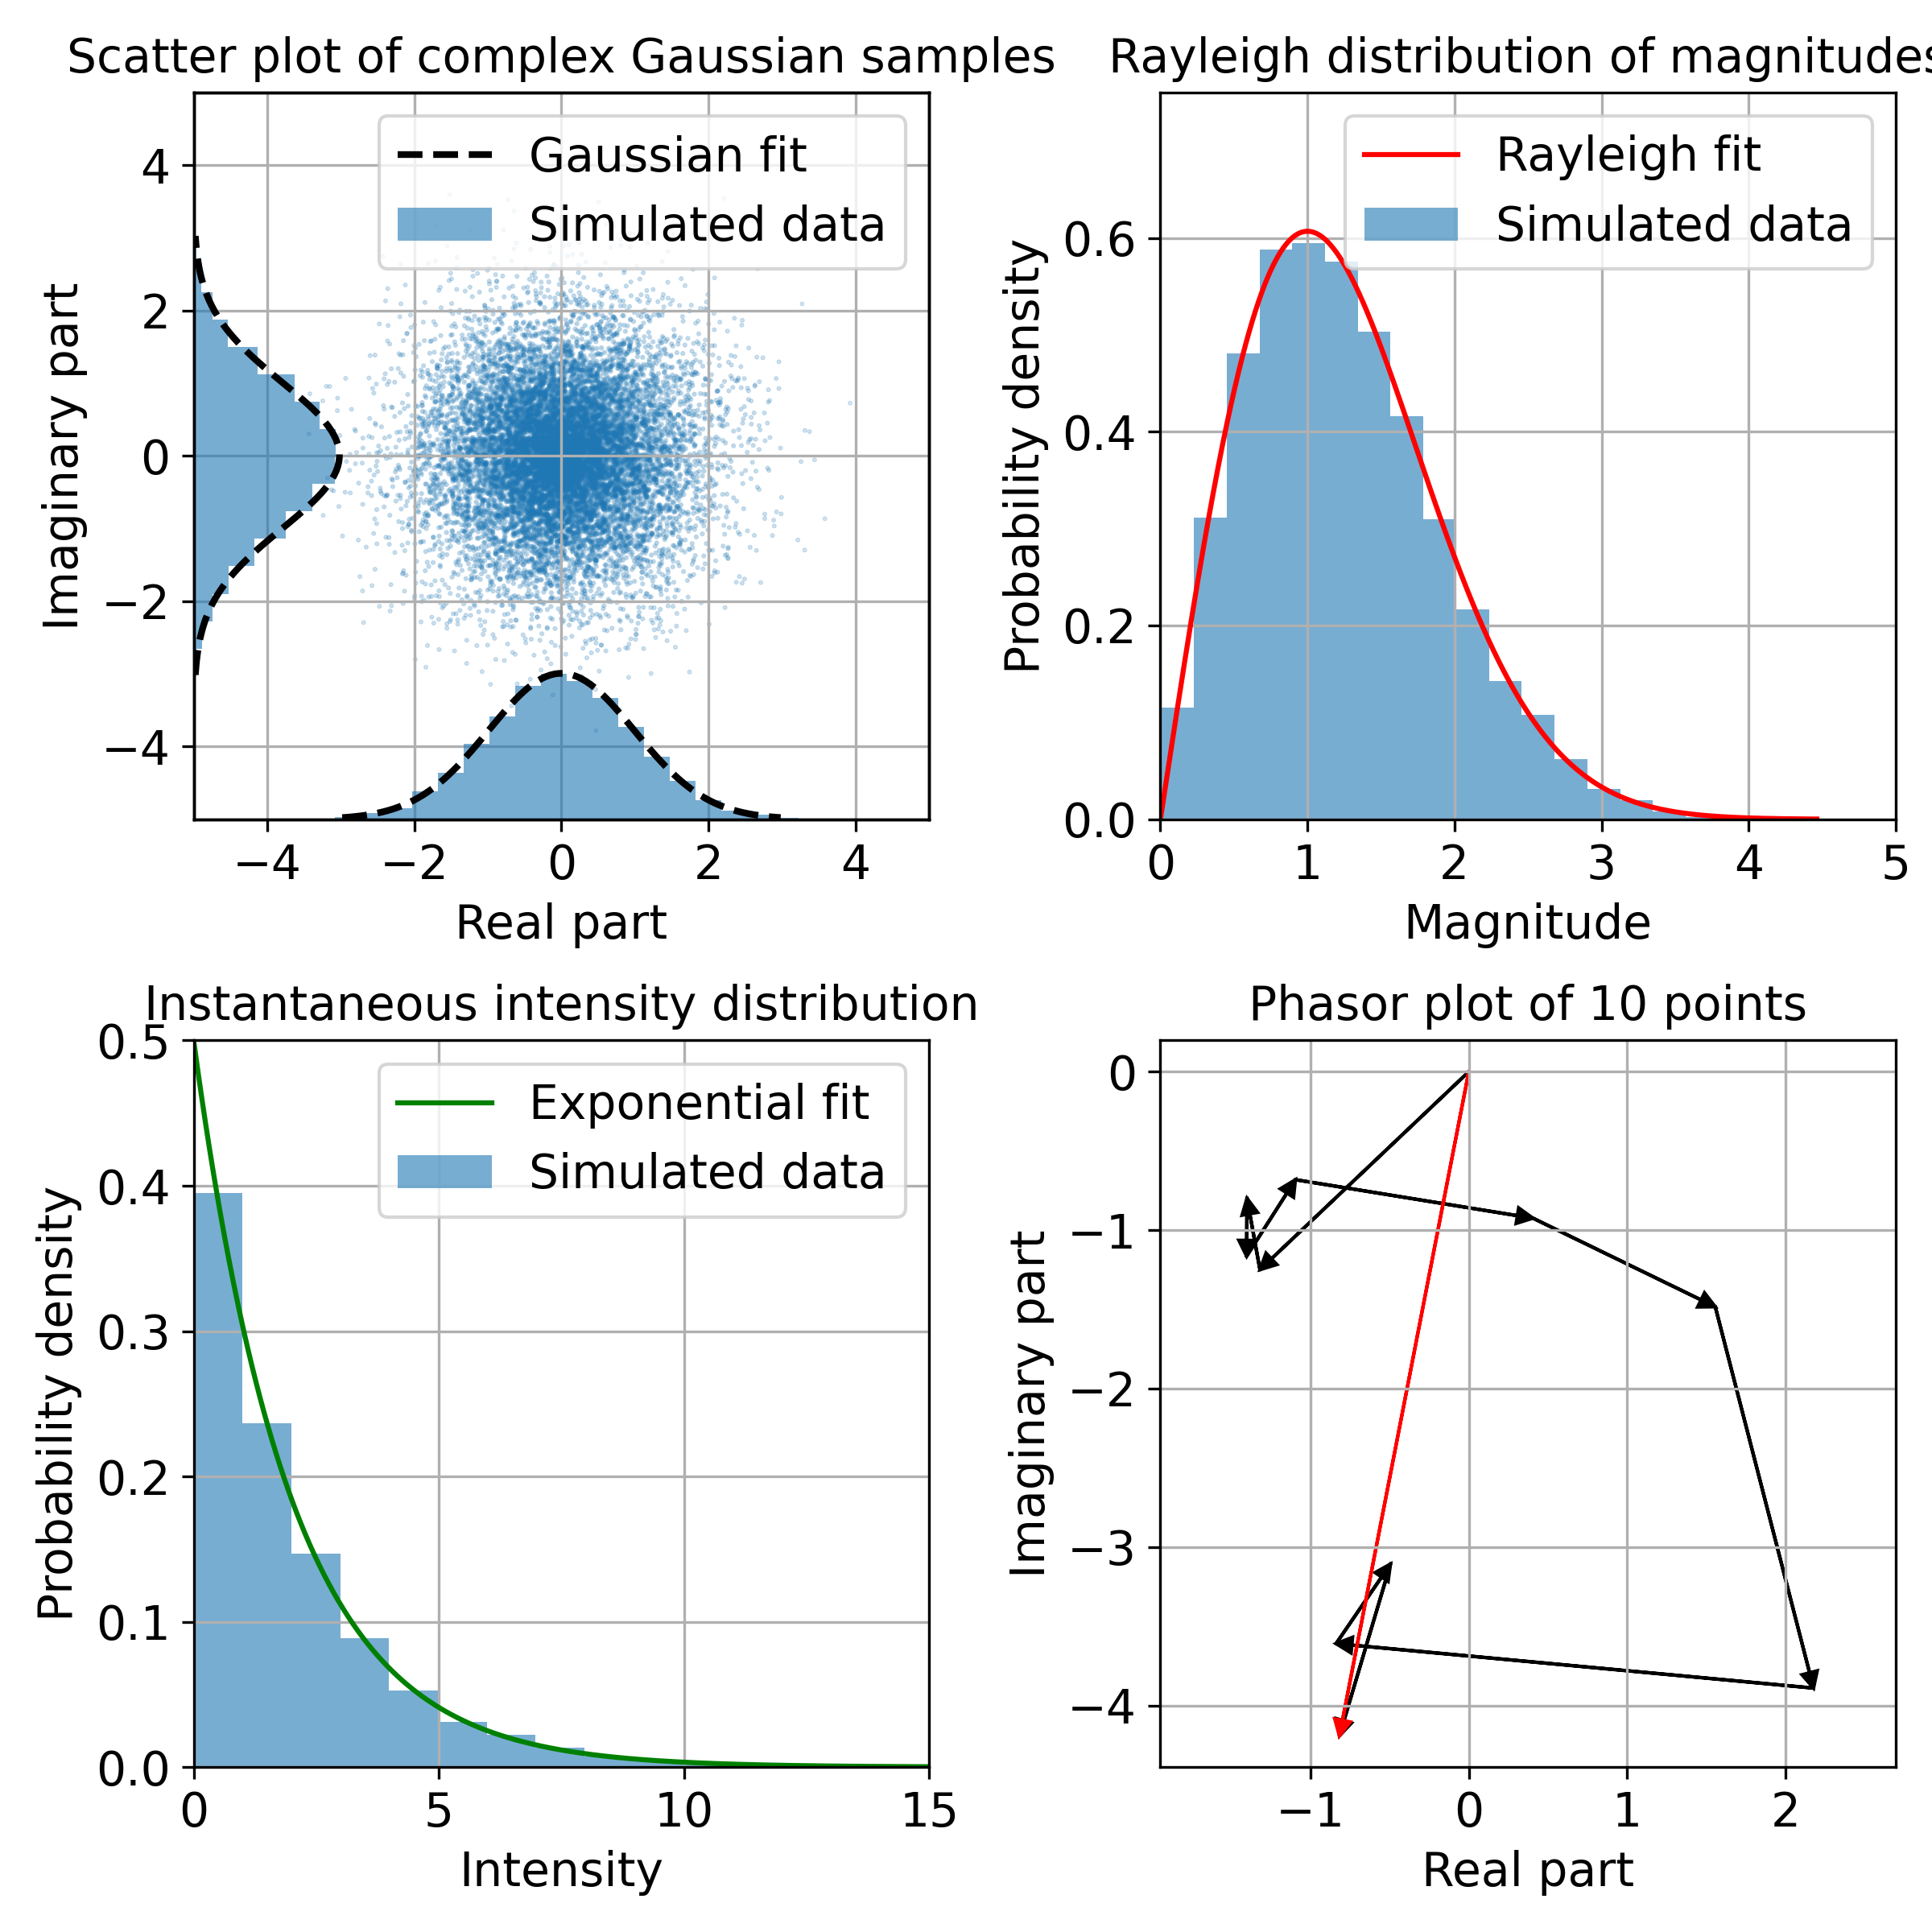
\includegraphics[width=0.75\linewidth]{content/images/Statistical_Optics/gaussian_process.png}
        \captionsetup{justification=centering}
        \caption{Gaussian random process visualisation, dispersion equals unity. Upper left subplot is 10000 samples marked at imaginary plane, upper right subplot Rayleigh distribution, lower left subplot negative exponent distribution, lower right subplot random phasor plotted from ten point.}
        \label{Fig:gaussian_process}
    \end{figure}
    This distribution is called the \textit{Rayleigh probability distribution}. In the last equation, the dependence on $\phi$ is not presented explicitly, which implies that the phase is distributed uniformly for all values ($0 \leq \phi \leq 2 \pi$), i.e.:
    \begin{align}
        p(\phi) = \cfrac{1}{\sqrt{2 \pi}}.
    \end{align}
    One can also consider probability density function for the \textit{instantaneous intensity}:
    \begin{align}
        I(t) = A^2(t)
    \end{align}
    and using the law for probability functions transformations I obtain:
    \begin{align}
        p(I) = \frac{1}{\langle I \rangle} e^{-I/\langle I \rangle},
    \end{align}
    where $\langle I \rangle = 2 \sigma$. This is distribution is negative exponential distribution. \rr{…and…need to have a conclusion}

    \rr{…it sounds ragged…}
    Gaussian random processes play a fundamental role in synchrotron radiation (SR) and self-amplified spontaneous emission free-electron laser (SASE FEL) radiation, and more generally, in statistical optics. From this point forward, I will assume that the processes dealt with in this thesis possess Gaussian statistics, with several exceptions discussed separately. Now, I will focus on extending the definition of stationarity to a broader class to account for the time-confined nature of SR and SASE FEL radiation.
    
\subsection{Quasi-stationary approximation}

    Although many day-to-day sources of radiation can be categorized as stationary or ergodic, non-stationary processes play a pivotal role in science. However, developing a generalized theory for non-stationary processes and deriving practical laws is very challenging. Nevertheless, there is a class of sources that can be described in the same manner similar to stationary ones. This kind of source are referred to as quasi-stationary. At this point, I will slightly deviate from the usual presentation of statistical optics concepts, like in~\cite{mandel_optical_1995, goodman_statistical_2015}, and delve into the concept of quasi-stationary. As the name suggests, quasi-stationary processes share the most of statistical properties with stationary ones, but they start and finish at specific points in time. Quasi-stationary processes appear to be stationary only within a certain interval of time, which is much smaller than their overall duration.
    
    So, if one observes radiation intensity at some point in space and record it over time then the ensemble average will be:
    \begin{align}
        I(t) \coloneqq \langle I(t) \rangle = \lim_{N\to\infty} \frac{1}{N}\sum_{i=1}^{N} E^{[i]}(t)E^{*[i]}(t)
    \end{align}
    $I(t)$ is the time envelope of the radiation and depends on time. Then I write the auto-correlation function:
    \begin{align}
        \Gamma(t_1, t_2) = \langle E(t_1)E^*(t_2) \rangle = \lim_{N\to\infty} \frac{1}{N}\sum_{i=1}^{N} E^{[i]}(t_1)E^{*[i]}(t_2)
    \end{align}
    At this point, I have not defined anything except for the fact that $I(t) \neq C$ and does depend on time, where $C$ is some constant. Then, introducing the normalized version of the auto-correlation function $\Gamma(t_1, t_2)$:
    \begin{align}
        g(t_1, t_2) = \frac{\langle E(t_1)E^*(t_2)\rangle}{\sqrt{\langle |E(t_1)|^2\rangle \langle |E^*(t_2)|^2\rangle}} = \frac{\Gamma(t_1, t_2)}{\sqrt{ I(t_1) I(t_2)}}.
    \end{align} 
    and rewriting this as: 
    \begin{align}
        \Gamma(t_1, t_2) = g(t_1, t_2) \sqrt{I(t_1) I(t_2)}.
    \end{align}
    I notice that for a quite large span of the process $g(t_2, t_1)$ only depends on the time difference $\Delta t = t_2 - t_1$. Having this, I obtain:
    \begin{align}
        \Gamma(t_1, t_2) = g(t_2 - t_1) \sqrt{I(t_1) I(t_2)}.
        \label{Eq:Strict_quasi_stationarity}
    \end{align}
    The radiation sources that have this kind of auto-correlation function I will call quasi-stationary, but there is a "weaker" definition of quasi-homogeneity. If one assumes that the width $g(t_2 - t_1)$ is much smaller than the scale of $I(t)$, then the result is an even simpler expression:
    \begin{align}
        \Gamma(t_1, t_2) = g(t_2 - t_1)I\bigg(\frac{t_1 + t_2}{2}\bigg)
        \label{Eq:weak_quasi_stationarity}
    \end{align}
    This representation of radiation sources is to some extent similar to quasi-homogeneity in the transverse domain~\cite{goodman_statistical_2015}. To my best knowledge, there are only a few mentions of Eq.~\ref{Eq:weak_quasi_stationarity}~\cite{lajunen_quasi-stationary_2006, ahad_quasi-monochromatic_2017} in optics community and authors of~\cite{geloni_statistical_2006} resulted in this expression for synchrotron radiation. Up to this point, I have not related these definition to real-world physical examples. First, I aim to derive another very useful properties of such processes and then provide an example, specifically, synchrotron radiation, which in most practical cases follows these definitions.

    \rr{…need to extend the content of this section a little bit}
    
\subsection{Cross-spectral density and generalized Wiener-Khinchin theorem}
    
    Continuing derivations, now I look at the correlation function in frequency domain. By definition I auto-correlate the Fourier images $\bar{E}(\omega)$ of the fields $E(t)$ at different frequencies $\omega_1$ and $\omega_2$:
    \begin{align}
        \langle \bar{E}(\omega_1)\bar{E}^*(\omega_2) \rangle = \frac{1}{(2 \pi)^2} \iint \limits_{-\infty}^{\infty} \langle E(t_1)E^*(t_2) \rangle e^{i \omega_1 t_1 - \omega_2 t_2} dt_1 dt_2, 
        \label{Eq:cross_spectral_density_dif}
    \end{align}
    where I brought the ensemble averaging under the integral sign. Then by using the expression Eq.~\ref{Eq:weak_quasi_stationarity} and substituting this in Eq.~\ref{Eq:cross_spectral_density_dif} I obtain:
    \begin{align}
        \langle \bar{E}(\omega_1)\bar{E}^*(\omega_2) \rangle = \frac{1}{(2 \pi)^2} \iint \limits_{-\infty}^{\infty}  g(t_2 - t_1)I\bigg(\frac{t_1 + t_2}{2}\bigg) e^{i \omega_1 t_1 - \omega_2 t_2} dt_1 dt_2.
    \end{align}
    I this point it makes sense to exchange variables $t_1, t_2$ for $\Delta t = t_2 - t_1$ and $\bar{t} = (t_2 + t_1)/2$. Now it is evident that it is possible to factorize the integral:
    \begin{align}
        \langle \bar{E}(\omega_1)\bar{E}^*(\omega_2) \rangle = \frac{1}{(2 \pi)^2} \int \limits_{-\infty}^{\infty}  g(\Delta t) e^{i \bar{\omega} \Delta t} d \Delta t  \int \limits_{-\infty}^{\infty} I(\bar{t}) e^{-i \Delta \omega \bar{t}} d\bar{t} = \bar{I}(\bar{\omega})f_{\omega}(\Delta \omega).
        \label{Eq:general_WKh_t}
    \end{align}
    This result in Eq.~\ref{Eq:general_WKh_t} I will refer to as the generalized Wiener-Khinchin theorem, although it is difficult to find this result elsewhere except for~\cite{geloni_statistical_2006} \rr{really? check again} in application to synchrotron radiation. A similar expression can be formulated for stationary radiation where $I(\bar{t})$ is constant $C$ and one obtains the integral:
    \begin{align}
        \langle \bar{E}(\omega_1)\bar{E}^*(\omega_2) \rangle = \frac{C}{(2 \pi)^2} \int \limits_{-\infty}^{\infty}  g(\Delta t) e^{i \bar{\omega} \Delta t} d \Delta t  \int \limits_{-\infty}^{\infty} e^{-i \Delta \omega \bar{t}} d\bar{t} = \bar{I}(\bar{\omega})\delta(\Delta \omega),
        \label{Eq:WKh_t_derivation}
    \end{align}
    where the latter integral equals the Dirac delta function: $\delta(\Delta \omega)$, and one can recognize that the radiation spectral density or just spectrum is related to the auto-correlation function via a Fourier transform.
    \begin{align}
        \bar{I}(\bar{\omega}) = \frac{1}{(2 \pi)^2} \int \limits_{-\infty}^{\infty}  g(\Delta t) e^{i \bar{\omega} \Delta t} d \Delta t,
        \label{Eq:WKh_t}
    \end{align}
    Both expression under Eqs.~\ref{Eq:general_WKh_t} and~\ref{Eq:WKh_t} play an essential role in coherence theory on an equal footing with the van Cittert-Zernike theorem, which I present in the next sections.

\section{Transverse coherence properties of quasi-stationary sources}
\label{Sec:Transverse coherence properties of quasi-stationary sources}
    
    Previously, I only considered sources in the time-frequency domain, while real fields exist in three-dimensional space. In this section, I will introduce transverse variables into the autocorrelation function. Then, I will classify the types of sources in terms of the factorizability of the cross-spectral density function, in a manner very similar to what I have done for the longitudinal domain. After this, I will provide proof of the van Cittert-Zernike theorem and its generalized version for quasi-homogeneous sources. This chapter will be the last one on the general laws of statistical optics, and it will be followed by practical applications of the theory to synchrotron and free-electron laser.

\subsection{Adding transverse domain}

    In the previous section, the signal was effectively observed through a pinhole. As I consider optical phenomena, not many of them truly occur only in the time-frequency domain -- the signal's propagation direction -- and extend into the transverse domains as well. Therefore, the expressions I previously provided should be adjusted accordingly to correctly reflect the statistical properties in transverse dimensions.
    Looking at Eq.~\ref{Eq:general_WKh_t},  I assume that $I(\bar{t})$ does not depend on transverse coordinates and I re-denote this distribution to $f(\bar{t})$. All the dependence on transverse variables $\vec{r}_1, \vec{r}_2$ goes to the $g_t$.
    \begin{align}
        \Gamma_{\omega}(\vec{r}_1, \vec{r}_2, \omega_1, \omega_2) = \frac{1}{(2 \pi)^2} \int \limits_{-\infty}^{\infty}  g_t(\vec{r}_1, \vec{r}_2, \Delta t) e^{i \bar{\omega} \Delta t} d \Delta t  \int \limits_{-\infty}^{\infty} f(\bar{t}) e^{-i \Delta \omega \bar{t}} d\bar{t} = G_{\omega}(\vec{r}_1, \vec{r}_2, \bar{\omega})\bar{f}(\Delta \omega),
        \label{Eq:}
    \end{align}    
    This representation results in the appearance of the cross-spectral density function $G_{\omega}(\vec{r}_1, \vec{r}_2, \bar{\omega})$ in a manner similar to that done for stationary sources but along with $\bar{f}(\Delta \omega)$ function that describes spectral correlation.

\subsection{Cross-spectral function distribution at the source}

    Continuing the reasoning on the transverse domain of the radiation, the normalized version of the cross-spectral density function has the following form:
    \begin{align}
        g(\vec{r}_1, \vec{r}_2, \omega; 0) = \frac{G(\vec{r}_1, \vec{r}_2, \omega; 0)}{\sqrt{I(\vec{r}_1, \omega; 0)I(\vec{r}_2, \omega; 0)}}.
    \end{align}
    Then, one can express cross-spectral density function as the following:
    \begin{align}
        G(\vec{r}_1, \vec{r}_2, \omega; 0) =  g(\Delta \vec{r}, \omega; 0){\sqrt{I(\vec{r}_1, \omega)I(\vec{r}_2, \omega; 0)}},
        \label{Eq:quasi_homogeneous_source_strong}
    \end{align}
    here I assumed that coherence length is distributed homogeneously across the intensity distribution in a similar way to what I have done in Eq.~\ref{Eq:Strict_quasi_stationarity}. This means that the width of $g(\Delta \vec{r}, \omega; 0)$ does not change across the intensity distribution. This kind of radiation source is called quasi-homogeneous according to another classical textbook~\cite{goodman_statistical_2015}. I can simplify the expression further and make further assumptions on the width of the $g(\Delta \vec{r}, \omega; 0)$ function to be much smaller than the radiation envelope $I(\bar{\vec{r}}, \omega; 0)$, again exactly similarly as was done for the longitudinal domain:
    \begin{align}
        G(\vec{r}_1, \vec{r}_2, \omega; 0) =  g(\Delta \vec{r}, \omega; 0)I(\vec{\bar{r}}, \omega).
        \label{Eq:quasi_homogeneous_source_weak}
    \end{align}
    In the limit case of fully incoherent source this degenerate to the following expression:
    \begin{align}
        G(\vec{r}_1, \vec{r}_2, \omega; 0) =  I(\vec{\bar{r}}, \omega; 0)\delta(\Delta \vec{r}),
        \label{Eq:incoherent_source}        
    \end{align}
    where the Dirac delta function is introduced. This kind of source describes fully incoherent sources or sources where the resolution of the optical system is larger than $g(\Delta \vec{r})$,~\cite{goodman_statistical_2015}.
    
\subsection{Propagation law for cross-spectral density function in free space}

    Another essential problem in coherence theory concerns the propagation of coherence properties through an optical system, which includes various optical elements interspaced with free space. By its nature, a single statistical realization of a field from a random process behaves identically to any other field and can be propagated in the same way, adhering to the wave equation. Looking ahead to the narrative of this thesis, one effective method to calculate the field and its statistical properties upon propagation is to directly apply the corresponding propagator—or a sequence of propagators—through the optical system. Although this approach is practical, it can also be somewhat cumbersome. It necessitates propagating each field sample separately or deriving an analytical expression for the corresponding propagator. Nevertheless, this method is used in many numerical codes for radiation propagation, including Synchrotron Radiation Workshop (SRW)~\cite{chubar_accurate_1998}.
 
    In the simplified scenario of just free space, it is possible to derive a highly useful law describing how the cross-spectral density function or the mutual coherence function evolves. This case is particularly applicable for estimating coherence properties at the entrance of the optical system. Typically, there is free space between the radiation source and the entrance of an optical system. I begin by examining the wave equation in free space:
    \begin{align}
        \nabla^2_1 \vec{E}(\vec{r}_1, t_1) - \cfrac{1}{c^2} \frac{\partial^2 \vec{E}(\vec{r}_1, t_1)}{\partial t_1^2} = 0
        \label{Eq:wave_eq}
    \end{align}
    By multiplying this with $\vec{E}^(\vec{r}_2, t_2)$, where $^*$ denotes the complex conjugate, and then incorporating it under the differentiation signs:
    \begin{align}
        \nabla^2_1 \big[\vec{E}(\vec{r}_1, t_1) \vec{E}(\vec{r}_2, t_2)\big]- \cfrac{1}{c^2} \frac{\partial^2 \big[\vec{E}(\vec{r}_1, t_1) \vec{E}(\vec{r}_2, t_2)\big]}{\partial t_1^2} = 0.
    \end{align}
    and then by ensemble averaging this equation, and noting that the averaging operation can be interchanged with differentiation, I obtain:
    \begin{align}
        \nabla^2_1 \Gamma(\vec{r}_1, \vec{r}_2, t_1, t_2)  - \cfrac{1}{c^2} \frac{\partial^2 \Gamma(\vec{r}_1, \vec{r}_2, t_1, t_2)}{\partial t_1^2} = 0,
    \end{align}
    To close this differential system, one can derive the complementary equation in the same manner:
    \begin{align}
        \nabla^2_2 \Gamma(\vec{r}_1, \vec{r}_2, t_1, t_2)  - \cfrac{1}{c^2} \frac{\partial^2 \Gamma(\vec{r}_1, \vec{r}_2, t_1, t_2)}{\partial t_2^2} = 0,
    \end{align}
    By taking the Fourier transform of both sides, I obtain a system for the cross-spectral density function $G(\vec{r}_1, \vec{r}_2, \omega)$ that is:
    \begin{align}
        \nabla^2_1 G(\vec{r}_1, \vec{r}_2, \omega) + k^2 G(\vec{r}_1, \vec{r}_2, \omega) = 0\\
        \nabla^2_2 G(\vec{r}_1, \vec{r}_2, \omega) + k^2 G(\vec{r}_1, \vec{r}_2, \omega) =0 .
    \end{align}
    where I divided each equation by $\bar{f}(\Delta \omega)$. This system of two Helmholtz equations has a known solution. Assuming that we know the distribution $G(\vec{r}'_1, \vec{r}'_2, \omega)$ in the $S$ plane, where $z=0$, we can solve this system using the Green's function for the Helmholtz equation with Dirichlet boundary conditions. This approach allows us to derive the following law for propagating the cross-spectral density function~\cite{mandel_optical_1995}:
    \begin{align}
        G(\vec{r}_1, \vec{r}_2, \omega) = \bigg(\cfrac{k}{ 2 \pi} \bigg)^2 \iint_{z=0} G(\vec{r}'_1, \vec{r}'_2, \omega) \cfrac{e^{i k (R_2 - R_1)}}{R_1 R_2} \cos(\theta_1) \cos(\theta_2) d^2r'_1 d^2r'_2
        \label{Eq:G_propagation_law}
    \end{align}
    \begin{wrapfigure}{r}{0.5\textwidth}
        \centering
        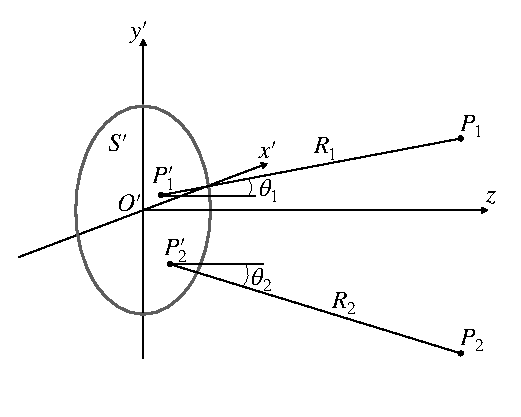
\includegraphics[width=0.95\linewidth]{content/images/Statistical_Optics/coh_prop_scheme.pdf}
        \captionsetup{justification=centering}
        \caption{Geometry of the cross-spectral density propagation in the free-space. Adapted from~\rr{cite}}
        \label{Fig:coh_prop_scheme}
    \end{wrapfigure}
    This expression is foundational for deriving the van Cittert-Zernike theorem, which I will discuss in the next section. Historically, the van Cittert-Zernike theorem was formulated using Huygens' principle, resulting in an expression for the mutual intensity function~\cite{van_cittert_wahrscheinliche_1934, zernike_concept_1938}. Interestingly, it should be noted that the cross-spectral density obeys the same laws as the mutual intensity function $J(\vec{r}_1, \vec{r}_2) = g_t(\vec{r}_1, \vec{r}_2, \Delta t = 0)$~\cite{goodman_statistical_2015, mandel_optical_1995}. It is important to remember that this holds true only for quasi-monochromatic sources. Therefore, I will continue to present the results for the theorem using the cross-spectral density.

\subsubsection{The van Cittert-Zernike theorem}
    Equation~\ref{Eq:G_propagation_law} is highly general and can be applied to any propagating field to calculate its cross-spectral distribution upon propagation. However, this integral can be further simplified to derive practical formulas for specific types of sources—namely, fully incoherent and partially coherent sources under the quasi-homogeneous approximation that I have introduced in Eqs.~\ref{Eq:quasi_homogeneous_source_weak},~\ref{Eq:incoherent_source}. 
    
    Assuming the paraxial approximation, I can write the following expression for the mutual intensity function derived from Eq.~\ref{Eq:G_propagation_law}:
    \begin{align}
        G(\vec{r}_1, \vec{r}_2, \omega) = \bigg(\cfrac{k}{ 2 \pi} \bigg)^2 \iint_{\mathcal{S}} G(\vec{r}'_1, \vec{r}'_2, \omega) \cfrac{e^{i k (R_2 - R_1)}}{R_1 R_2}d^2r'_1 d^2r'_2
        \label{Eq:G_propagation_law_4_VCZ}
    \end{align}
    \begin{figure}[h!]
        \centering
        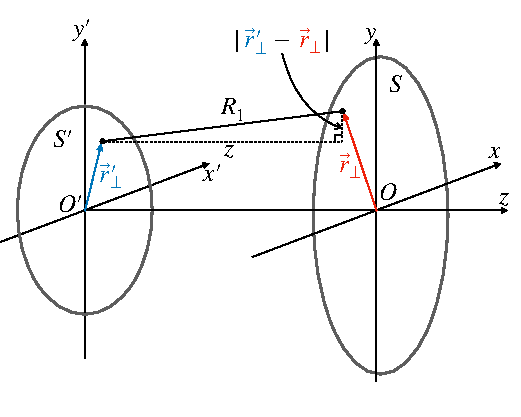
\includegraphics[width=0.5\linewidth]{content/images/Statistical_Optics/coh_prop_scheme_2.pdf}
        \captionsetup{justification=centering}
        \caption{Geometry of the cross-spectral density propagation in the free-space. Adapted from~\rr{cite}.}
        \label{Fig:coh_prop_scheme_2}
    \end{figure}
    If the cross-spectral density function is observed in the far zone Eq.~\ref{Eq:G_propagation_law_4_VCZ} can be further simplified using the relations:
    \begin{align}
        \begin{array}{c}
            R_{1, 2}\approx  z + \cfrac{|\vec{r}'_{1, 2{\perp}} - \vec{r}_{1, 2{\perp}}|^2}{2z}\\
            \\
            R_{1}R_{1} \approx z^2
        \end{array}
        \label{Eq:R1R2_simp}
    \end{align}
    for simplicity of the notation it make sense to redefine $\vec{r}_{1, 2} :=\vec{r}_{1, 2{\perp}}$ and the same for $\vec{r}'_{1, 2} :=\vec{r}'_{1, 2{\perp}}$ (but only till the end of the current Section).

    Now I would like to simplify $R_2 - R_1$ in the exponent. Using first relation in Eq.~\ref{Eq:R1R2_simp}:
    \begin{align}
        R_2 - R_1 = \cfrac{1}{2z} \bigg(|\vec{r}_{2}|^2 - 2|\vec{r}_{2} \cdot \vec{r}'_{2}| + |\vec{r}'_{2}|^2 - |\vec{r}_{1}|^2 + 2|\vec{r}_{1} \cdot \vec{r}'_{1}| - |\vec{r}'_{1}|^2\bigg)
    \end{align} 
    and introducing new variables $\vec{\bar{r}} = \vec{r}_1 - \vec{r}_2$ and $\Delta\vec{r} = (\vec{r}_2 + \vec{r}_1)/2$ and the same for the primed set of variables, this leads me to: 
    \begin{align}
        \begin{array}{c}
        |\vec{r}_{2}|^2 - |\vec{r}_{1}|^2 = -2\vec{\bar{r}}\cdot\Delta\vec{r} \\
        |\vec{r}'_{2}|^2 - |\vec{r}'_{1}|^2 = -2\vec{\bar{r}}'\cdot\Delta\vec{r}' \\
        |\vec{r}_{1} \cdot \vec{r}'_{1}| - |\vec{r}_{2} \cdot \vec{r}'_{2}| = \vec{\bar{r}}\cdot\Delta\vec{r}' + \vec{\bar{r}}'\cdot\Delta\vec{r},
        \end{array}
    \end{align}
    where $\_ \cdot \_$ denotes the scalar product. Then I substitute this in Eq.~\ref{Eq:G_propagation_law_4_VCZ} and obtain:
    \begin{align}
        G(\vec{\bar{r}}, \Delta\vec{r}, \omega; 0) = \bigg(\cfrac{k}{ 2 \pi} \bigg)^2 \cfrac{e^{-\frac{i k}{z} \vec{\bar{r}}\cdot\Delta\vec{r}}}{z^2}     \iint_{\mathcal{S}} G(\vec{\bar{r}}', \Delta\vec{r}', \omega, z) e^{\frac{i k}{z} (\vec{\bar{r}}\cdot\Delta\vec{r}' + \Delta\vec{r}\cdot\vec{\bar{r}}')} d\vec{\bar{r}}' d\Delta\vec{r}' 
        \label{Eq:VCZ_general_form}
    \end{align}
    Here, I neglected the term $2\vec{\bar{r}}'\cdot\Delta\vec{r}'$ in the exponent under assumption condition $\vec{\bar{r}}'\cdot\Delta\vec{r}'/ (\lambda z) \ll 1$, which basically can be interpreted as placing the observation plane ($S'$) in far zone.
    
    Using this definition of fully incoherent source and substituting this in Eq.~\ref{Eq:VCZ_general_form} I obtains:
    \begin{align}
        G(\vec{\bar{r}}, \Delta\vec{r}, \omega; z) &= \cfrac{e^{- i \frac{k}{z} \vec{\bar{r}}\cdot\Delta\vec{r}}}{(\lambda z)^2} \iint_{\mathcal{S}} I(\vec{\bar{r}}', \omega)\delta(\Delta \vec{r}') e^{i \frac{k}{z} (\vec{\bar{r}}\cdot\Delta\vec{r}' + \vec{\bar{r}}'\cdot\Delta\vec{r})} d\vec{\bar{r}}' d\Delta\vec{r}' \nonumber = \\
        &\fcolorbox{black}{yellow!30}{\rule[-4ex]{0pt}{10ex}$\displaystyle \stackrel{\text{van Cittert-Zernike theorem}}{\cfrac{e^{-i \frac{k}{z} \vec{\bar{r}}\cdot\Delta\vec{r}}}{(\lambda z)^2} \int_{\mathcal{S}} I(\vec{\bar{r}}', \omega) e^{i \frac{k}{z} \vec{\bar{r}}'\cdot\Delta\vec{r}} d\vec{\bar{r}}'}$}
        \label{Eq:VCZ_incoherent}
    \end{align}
    This is the original result of the van Cittert-Zernike theorem but the theorem can be extended for a more general source representation under Eq.~\ref{Eq:quasi_homogeneous_source_weak}. Again using integral in Eq.~\ref{Eq:VCZ_general_form} and substituting in it the expression from Eq.~\ref{Eq:quasi_homogeneous_source_weak} I obtain:
    \begin{align}
        G(\vec{\bar{r}}, \Delta\vec{r}, \omega; z) &=  \cfrac{e^{-i \frac{k}{z} \vec{\bar{r}}\cdot\Delta\vec{r}}}{(\lambda z)^2} \iint_{\mathcal{S}} g(\Delta \vec{r}', \omega; 0)I(\vec{\bar{r}}', \omega) e^{i \frac{k}{z} (\vec{\bar{r}}\cdot\Delta\vec{r}' + \vec{\bar{r}}'\cdot\Delta\vec{r})} \, d\vec{\bar{r}}' \, d\Delta\vec{r}' \nonumber =\\
        &\fcolorbox{black}{yellow!30}{\rule[-4ex]{0pt}{10ex}$\displaystyle \stackrel{\text{generalised van Cittert-Zernike theorem}}{\cfrac{e^{-i \frac{k}{z} \vec{\bar{r}}\cdot\Delta\vec{r}}}{(\lambda z)^2} \int_{\mathcal{S}} g(\Delta \vec{r}', \omega; 0) e^{-i \frac{k}{z} \vec{\bar{r}}\cdot\Delta\vec{r}'} \, d\Delta\vec{r}'  \int_{\mathcal{S}} I(\vec{\bar{r}}', \omega) e^{i \frac{k}{z} \vec{\bar{r}}'\cdot\Delta\vec{r}} \, d\vec{\bar{r}}'}$}
        \label{Eq:VCZ_partially_coherent}
    \end{align}
    \begin{figure*}[h!]
      \centering
      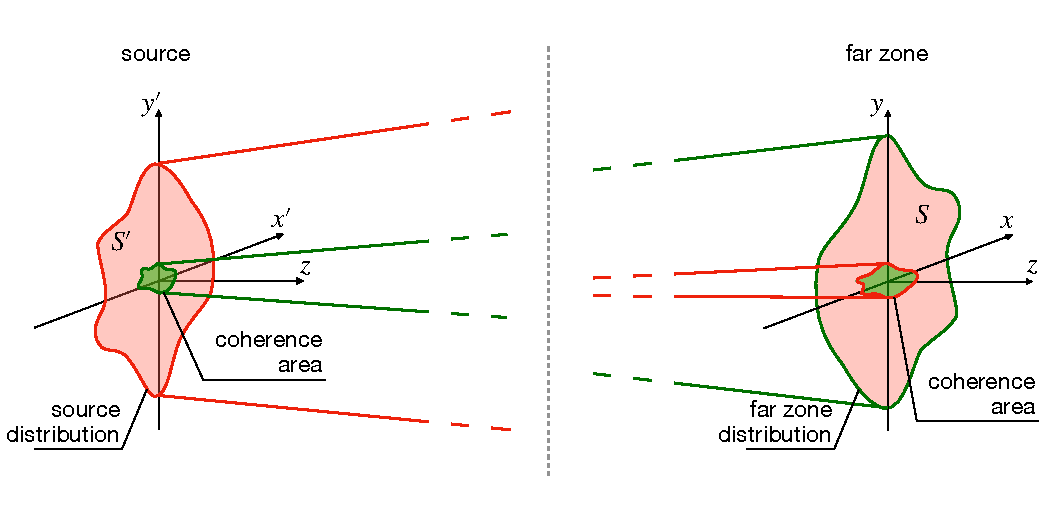
\includegraphics[width=0.95\linewidth]{content/images/Statistical_Optics/VCZ_scheme.pdf}
      \captionsetup{justification=centering}
      \caption{Visual representation of the generalised van Cittert-Zernike theorem. }
      \label{Fig:coh_prop_scheme}
    \end{figure*}
    \begin{figure}[h!]
        \centering
        \begin{tikzpicture}[
            % Define styles
            node distance=2cm,
            mynode/.style={
              shape=ellipse,
              draw,
              text width=2.5cm,
              align=center
            },
            bluearrow/.style={
              <->,
              >=latex,
              blue,
              thick
            },
            redarrow/.style={
              <->,
              >=latex,
              red,
              thick
            },
            bluetext/.style={
              text=blue
            },
            redtext/.style={
              text=red
            }
          ]
        
          % Nodes
          \node[mynode] (g0) {$g(\Delta\mathbf{\hat{r}}; \mathbf{0})$};
          \node[mynode, right=of g0] (I0) {$I(\mathbf{\hat{r}}; \mathbf{0})$};
          \node[mynode, below=of g0] (gz) {$\dfrac{g( \Delta\mathbf{\hat{\theta}}; \mathbf{\hat{z}})}{\exp[i\mathbf{\hat{z}} \Delta\mathbf{\hat{\theta}} \cdot \mathbf{\theta}]}$};
          \node[mynode, right=of gz] (Iz) {$I(\mathbf{\hat{\theta}}; \mathbf{\hat{z}})$};
        
          % Arrows with FT labels
          \draw[bluearrow] (g0) -- (Iz) node[pos=0.25, above, bluetext] {FT};
          \draw[redarrow] (gz) -- (I0) node[pos=0.75, above, redtext] {FT};
        \end{tikzpicture}
        \caption{Relations between intensity and cross-spectral distributions at the source and in the far zone that van Cittert-Zernike theorem and its inverse version set.}
        \label{Fig:VCZ_scheme}
    \end{figure}
    This is a result for a partially coherent source with cross-spectral density distribution as given in Eq.~\ref{Eq:quasi_homogeneous_source_weak}. Surely, it is easy to show that the inverse version of the van Cittert-Zernike theorem holds as well. So, I present all the relations in the diagram in Fig.~\ref{Fig:VCZ_scheme}. The van Cittert-Zernike theorem (and its generalized version) provides a very practical relation between the source size and the observed coherence spot in the far zone and forms the basis for coherence theory for studying synchrotron radiation sources.

    \rr{discuss more on the results}

\section{Coherence properties of synchrotron radiation}

    In this section, I will explore the general theory of synchrotron radiation coherence, following the framework presented in~\cite{geloni_statistical_2006}. This framework results in practical expressions for calculating the correlation function that are well-suited for numerical implementation. This numerical implementation resembles Monte-Carlo-like methods, where the contribution from each particle is calculated separately and then summed up. This is discussed in detail in the corresponding sections of Paper II.

    Based on the theory developed in this section, I will provide the theoretical reasoning and introduce algorithms for calculating radiation using Gaussian field generators based on white noise \rr{again, Gaussian noise, white noise? should be one term across the thesis} later in the chapter. First, I present an algorithm for fully incoherent radiation and demonstrate its application in Paper I, focusing on the image formation properties of a pinhole camera at a synchrotron facility. Then, I extend it to the case of partially coherent radiation and present the results in Paper II, followed by Paper III, where I consider an algorithm for generating radiation with arbitrary phase space distribution. Each development stage of the algorithm will be preceded by a dedicated "heuristic" section, outlining the idea behind the algorithm.

    The classical textbook on statistical optics~\cite{mandel_optical_1995} provides a wave equation for radiation from a fluctuating scalar source in the following form:
    \begin{align}
        c^2 \nabla^2 \vec{E}(\vec{r}, t) - \frac{\partial^2 \vec{E}(\vec{r}, t)}{\partial t^2} = -4 \pi c^2 Q(\vec{r}, t).
        \label{Eq:mandel_Eq}
    \end{align}
    It then provides an expression for propagating the radiation from the source based on the propagation law of the correlation function. This means that the correlation function at some position along the optical axis can be expressed as an integral using the correlation function of the source:
    \begin{align}
        \Gamma_Q(\vec{r}_1, \vec{r}_2, t_1, t_2) = \langle  Q(\vec{r}_1, t_1)  Q^*(\vec{r}_2, t_2) \rangle.
        \label{Eq:wave_eq_Mandel}
    \end{align}
    \rr{STOPPED HERE}
    This calculation is complicated by the fact that the nature of $Q(\vec{r}, t)$ remains obscured. For example, to describe a thermal source, radiation must be calculated using quantum mechanics, making it unclear how to properly present the wave equation in Eq.~\ref{Eq:wave_eq_Mandel}. Fortunately, synchrotron radiation from a relativistic electron beam is governed solely by classical electrodynamics, allowing for writing an explicit equation in the same manner as Eq.~\rr{}, but accounting for the whole electron beam:
    \begin{align}
        c^2 \nabla^2 \vec{E} - \frac{\partial^2 \vec{E}}{\partial t^2} = - 4 \pi c^2 \vec{\nabla} (-e) \sum_{i=1}^{N_e}\delta(\vec{r} - \vec{r}_i'(t)) + 4 \pi (-e) \sum_{i=1}^{N_e}\frac{\partial (\vec{v}_i(t)\delta(\vec{r} - \vec{r}_i'(t)))}{\partial t}.
    \end{align}
    This equation represents a stochastic partial differential equation where the right-hand side depends on random variables, such as the coordinates and velocities of electrons within the electron beam's phase space. Solving this equation in the context of stochastic partial differential equations demands substantial analytical effort, if not impossible at the current moment.

    This problem can be simplified by employing the superposition principle of electrodynamics. As demonstrated in Chapter~\ref{Chapter:Undulator radiation imaginary source peculiarities}, one can easily solve the equation for a single electron. One can obtain the final solution for the field by summing up the contributions from all electrons. In numerical simulations, this approach requires solving $N_e \times N_b$ equations for single electrons, where $N_e$ is the number of electrons and $N_b$ is the number of statistical realizations. Nevertheless, analytically, this approach can lead to very useful and practical equations for the coherence properties of synchrotron radiation, which I will discuss in the next section.
    
\subsection{Cross-spectral density functions for synchrotron radiation}   
    
    This section mainly follows the reasoning given in~\cite{geloni_statistical_2006}. As it has been discussed, the field from the whole electron beam can be written as the sum of the field of individual electrons:
    \begin{align}
        E_b(z, \vec{r}, t) = \sum_{k=1}^{N_e} E(\vec{\eta}_k, \vec{l}_k, z, \vec{r}, t - t_k), 
    \end{align}
    where $\vec{\eta}_k$ is an electron deflection, $\vec{l}_k$ its offset and $t_k$ -- arrival time with respect to some reference time. It is more practical to consider this field in frequency domain that will be rewritten as the following: 
    \begin{align}
        \bar{E}_b(z, \vec{r}, \omega) = \sum_{k=1}^{N_e} \bar{E}(\vec{\eta}_k, \vec{l}_k, z, \vec{r}, \omega)e^{i \omega t_k}.
        \label{Eq:ebeam_rad_omega}
    \end{align}   
    Here I note that all $\bar{E}$ have the same distribution for all $k$ and have finite mean and dispersion. Additionally, the arrival times of the electrons $t_k$ are statistically independent of each other and do not depend on $\vec{\eta}_k, \vec{l}_k$.
    
    I assume that the length of the electron beam $\sigma_T c$ is much larger than the wavelength: \rr{$\omega \sigma_T \ll 1$ ??}. This leads to the approximation that the phase is distributed uniformly in the interval $(0, 2\pi)$. The case $\omega \sigma_T \gg 1$ refers to an effect called coherent synchrotron radiation (CSR), which I do not consider in this thesis.
    
    With these assumptions, I can prove that the field $\bar{E}_b(z, \vec{r}, \omega)$ actually follows complex Gaussian random process statistics, or simply saying throughout this thesis Gaussian statistics. Indeed, with the help of the central limit theorem, it is clear that the sum of the random functions in Eq.~\ref{Eq:ebeam_rad_omega} will result in the real and imaginary parts of $\bar{E}_b$ following Gaussian statistics.
    
    Writing the cross-spectral density function of the first order of the field $\bar{E}_b$:
    \begin{align}
        \Gamma_\omega (z, \vec{r}_1, \vec{r}_2, \omega_1, \omega_2) = \langle \bar{E}_b(z, \vec{r}_1, \omega_1) \bar{E}^*_b(z, \vec{r}_1, \omega_1) \rangle,
        \label{Eq:Gamma_omega}
    \end{align} 
    and substituting Eq.~\ref{Eq:ebeam_rad_omega} in Eq.~\ref{Eq:Gamma_omega} I obtain:
    \begin{align}
        \Gamma_\omega (z, \vec{r}_1, \vec{r}_2, \omega_1, \omega_2) = \bigg\langle 
        \sum_{m,n=1}^{N_e} \bar{E}(\vec{\eta}_m, \vec{l}_m, z, \vec{r}, \omega_1)\bar{E}^*(\vec{\eta}_n, \vec{l}_n, z, \vec{r}, \omega_2)e^{i (\omega_1 t_m - \omega_2 t_n)}
        \bigg\rangle
    \end{align}
    At this point, it is worth noting that higher-order correlation functions of a Gaussian random process can be expressed with the help of the moment theorem, as mentioned in Section~\ref{Sec:Gaussian random processes}. This is a fundamental property of Gaussian random processes and a central one for this thesis.
    
    Continuing with the derivation, I extract the sum over the same indexes and obtain:
    \begin{align}
        \Gamma_\omega (z, \vec{r}_1, \vec{r}_2, \omega_1, \omega_2) =  
        \sum_{m = 1}^{N_e} \langle\bar{E}(\vec{\eta}_m, \vec{l}_m, z, \vec{r}, \omega_1)\bar{E}^*(\vec{\eta}_m, \vec{l}_m, z, \vec{r}, \omega_2)e^{i (\omega_1 -\omega_2) t_m)}\rangle + \cr
        \sum_{m \neq n}^{N_e} \langle\bar{E}(\vec{\eta}_m, \vec{l}_m, z, \vec{r}, \omega_1)\bar{E}^*(\vec{\eta}_n, \vec{l}_n, z, \vec{r}, \omega_2)e^{i (\omega_1 t_m - \omega_2 t_n)}\rangle.
        \label{Eq:Two_sums}
    \end{align}
    One may notice that ensemble average $\langle e^{i \omega t_k}\rangle = \int\limits_{-\infty}^{\infty} f(t_k) e^{i \omega t_k} dt_k = \bar{f} (\omega)$ according to the definition of the statistical realisation in Eq.~\ref{Eq:ensemble_int_avr}. So, I can rewrite Eq.~\ref{Eq:Two_sums} as the following:
    \begin{align}
        \Gamma_\omega (z, \vec{r}_1, \vec{r}_2, \omega_1, \omega_2) =  
        \sum_{m = 1}^{N_e} \langle\bar{E}(\vec{\eta}_m, \vec{l}_m, z, \vec{r}, \omega_1)\bar{E}^*(\vec{\eta}_m, \vec{l}_m, z, \vec{r}, \omega_2) \rangle\bar{f}(\omega_1 - \omega_2) + \cr
        \sum_{m \neq n}^{N_e} \langle\bar{E}(\vec{\eta}_m, \vec{l}_m, z, \vec{r}, \omega_1)\bar{E}^*(\vec{\eta}_n, \vec{l}_n, z, \vec{r}, \omega_2)\rangle\bar{f}(\omega_1)\bar{f}(-\omega_2).
        \label{Eq:Two_sums}
    \end{align}
    The second term corresponds to the "interference" term between radiation from different electrons. I assumed that $\sigma_T \omega \gg 1$, which means that the width of $\bar{f}(\omega)$ is much smaller than bandwidth of the radiation and product $\bar{f}(\omega_1)\bar{f}(-\omega_2)$ rapidly goes to zero as one increases the difference $\omega_2 - \omega_1$. So, I can neglect this term and obtain: 
    \begin{align}
        \Gamma_\omega (z, \vec{r}_1, \vec{r}_2, \omega_1, \omega_2) =  
        \sum_{m = 1}^{N_e} \langle\bar{E}(\vec{\eta}_m, \vec{l}_m, z, \vec{r}, \omega_1)\bar{E}^*(\vec{\eta}_m, \vec{l}_m, z, \vec{r}, \omega_2) \rangle\bar{f}(\omega_1 - \omega_2).
        \label{Eq:}
    \end{align}
    To express the equation more concisely, I note that the ensemble-averaged quantity does not depend on a particular electron, thus I write:
    \begin{align}
        \Gamma_\omega (z, \vec{r}_1, \vec{r}_2, \omega_1, \omega_2) =
        N_e \bar{f}(\omega_1 - \omega_2) \langle\bar{E}(\vec{\eta}, \vec{l}, z, \vec{r}, \omega_1)\bar{E}^*(\vec{\eta}, \vec{l}, z, \vec{r}, \omega_2) \rangle.
        \label{Eq:}
    \end{align} 
    Also, following the ensemble averaging definition, I can write it via a double integral as follows:
    \begin{align}
        \Gamma_\omega (z, \vec{r}_1, \vec{r}_2, \omega_1, \omega_2) = N_e \bar{f}(\omega_1 - \omega_2) \iint \limits_{-\infty}^{\infty}f_{l}(\vec{l}) f_{\eta}(\vec{\eta}) \bar{E}(\vec{\eta}, \vec{l}, z, \vec{r}, \omega_1)\bar{E}^*(\vec{\eta}, \vec{l}, z, \vec{r}, \omega_2)d\vec{l} d\vec{\eta}.
        \label{Eq:}
    \end{align} 
    or explicitly as a sum following the alternative definition of ensemble averaging:
    \begin{align}
        \Gamma_\omega (z, \vec{r}_1, \vec{r}_2, \omega_1, \omega_2) = 
        N_e \bar{f}(\omega_1 - \omega_2) \sum_{k = 1}^{N}\bar{E}(\vec{\eta}_k, \vec{l}_k, z, \vec{r}, \omega_1)\bar{E}^*(\vec{\eta}_k, \vec{l}_k, z, \vec{r}, \omega_2),
        \label{Eq:}
    \end{align} 
    where $N$ is an integer number and sufficiently large. As one can see here, the radiation from different electrons is correlated only with itself. This is a consequence of dropping the term with $\bar{f}(\omega_1)\bar{f}(-\omega_2)$. Thus, the calculation of $\Gamma_\omega (z, \vec{r}_1, \vec{r}_2, \omega_1, \omega_2)$ requires knowledge of the electron beam phase space distribution $f_{l}(\vec{l}) f_{\eta}(\vec{\eta})$ and radiation from a single electron, $\bar{E}(\vec{\eta}, \vec{l}, z, \vec{r}, \omega)$, accounting for an arbitrary tilt and shift of the electron.
        
    In the last equation, the variation of $\bar{E}$ with respect to $\omega$ is slow enough on the scale of $\bar{f}$, so I can use $\omega_1$ in $\bar{E}^*(\vec{\eta}, \vec{l}, z, \vec{r}, \omega_1)$ instead of $\omega_2$. To justify this, one should look at the width scales: the width of $\bar{f}$ is proportional to $1/\sigma_T$ and the electric field resonance width amounts to $\omega_r/N_w$, where $\omega_r$ is the resonance frequency. Considering a numerical example for X-ray, I take the wavelength to be $1$~$\AA$, the number of undulator periods $N_w = 10^2$, and the duration of the electron beam $\sigma_T = 5$~ps according to the PETRA IV conceptual design report\cite{cite}. One has $\omega_r/N_w \sim 2 \times 10^{17}$, and $1/\sigma_T \sim 2 \times 10^{11}$, and as one can see, $\omega_r/N_w \gg 1/\sigma_T$. As a result, I obtain the following expression for the correlation function in the frequency domain:
    \begin{align}
        \Gamma_\omega (z, \vec{r}_1, \vec{r}_2, \omega_1, \omega_2) = N_e \bar{f}(\omega_1 - \omega_2) G(z, \vec{r}_1, \vec{r}_2, \omega_1).
        \label{Eq:Correlation_function_und_radiation}
    \end{align}
    where $G(z, \vec{r}_1, \vec{r}_2, \omega)$
    \begin{align}
        G(z, \vec{r}_1, \vec{r}_2, \omega) = \langle\bar{E}(\vec{\eta}, \vec{l}, z, \vec{r}, \omega)\bar{E}^*(\vec{\eta}, \vec{l}, z, \vec{r}, \omega) \rangle.
        \label{Eq:Cross_spectral_density_und_radiation}
    \end{align}
    It is worth mentioning that spatial and frequency domains coherence features are factorised. 
    
    Usually, synchrotron radiation is seen through an monochromator with \rr{transfer?} function $T(\omega)$, so one needs to rewrite Eq.~\ref{Eq:Correlation_function_und_radiation}: 
    \begin{align}
        \Gamma_\omega (z, \vec{r}_1, \vec{r}_2, \omega_1, \omega_2) = N_e \bar{f}(\omega_1 - \omega_2) G(z, \vec{r}_1, \vec{r}_2, \omega_1) T(\omega_1) T(\omega_2)
        \label{Eq:Cross_spectral_density_und_radiation_mono}
    \end{align}
    I notice here that in this expression, spatial and frequency coherence features are separated. In the next section, I will show that the relation of the frequency and time domain correlation functions follows a similar relation as the generalized Wiener–Khinchin theorem in Eq.~\ref{Eq:general_WKh_t}.
    
\subsection{Consistency of quasi-stationary approximation and Wiener–Khinchin theorem for synchrotron radiation}
    
    To show that Eq.~\ref{Eq:Cross_spectral_density_und_radiation_mono} describes a source with similar properties as the one under Eq.~\ref{Eq:general_WKh_t}, one needs to perform a Fourier transform to the time domain:
    \begin{align}
        \Gamma_t(z, \vec{r}_1, \vec{r}_2, t_1, t_2) = 
        \frac{1}{(2 \pi)^2}\iint \limits_{-\infty}^{\infty} \Gamma_\omega (z, \vec{r}_1, \vec{r}_2, \omega_1, \omega_2) e^{-i\omega_1 t_1} e^{i\omega_2 t_2} d\omega_1 d\omega_2 = \cr
        \frac{N_e}{(2 \pi)^2}\iint \limits_{-\infty}^{\infty} \bar{f}(\omega_1 - \omega_2) G(z, \vec{r}_1, \vec{r}_2, \omega_1) T(\omega_1) T(\omega_2) e^{-i\omega_1 t_1} e^{i\omega_2 t_2} d\omega_1 d\omega_2
    \end{align}
    This radiation is seen through a monochromator that has the bandwidth $\Delta \omega_m$ around the frequency $\omega_0$. In the case when the monochromator bandwidth $\Delta \omega_m$ is much larger than the typical scale of the width of $\bar{f}$, $\Delta \omega_m \gg 1/\sigma_T$, I can conclude that $T$ does not vary much on the scale of $\bar{f}$, and then I can write that $T(\omega_1) T(\omega_2) = |T(\bar{\omega})|^2$, which leads me to the following expression:
    \begin{align}
        \Gamma_t(z, \vec{r}_1, \vec{r}_2, t_1, t_2) = 
        \frac{N_e}{(2 \pi)^2}\int \limits_{-\infty}^{\infty} \bar{f}(\Delta \omega) e^{-i\Delta \omega \bar{t}}d\Delta \omega \int \limits_{-\infty}^{\infty} G(z, \vec{r}_1, \vec{r}_2,\bar{\omega}) T(\bar{\omega}) e^{i\bar{\omega} \Delta t}d\bar{\omega} = \cr
        g_t(\vec{r}_1, \vec{r}_2, \Delta t) f(\bar{t}).
    \end{align}
    In this expression, I separated two integrals. One can see that this result is a recurrence of the generalized Wiener-Khinchin theorem~\ref{Eq:general_WKh_t} but inverse.

\subsection{Quasi-homogeneity approximation for synchrotron radiation}

    As one can see, synchrotron radiation in many practical cases, especially in the X-ray range, behaves as a quasi-stationary source. We can write the cross-spectral density function in the standard form used in statistical optics, $G(z, \vec{r}_1, \vec{r}_2, \bar{\omega})$. Recalling the definition of quasi-homogeneity from Eq.~\ref{Eq:quasi_homogeneous_source_strong}, i.e. $G(\vec{r}_1, \vec{r}_2, \omega; 0) =  g(\Delta \vec{r}, \omega; 0)I(\vec{\bar{r}}, \omega)$, it is reasonable to assume that synchrotron radiation generally follows this definition. In other words, the width of $g(\Delta \vec{r}, \omega; 0)$ remains constant across the radiation intensity distribution. A proof for this can be found in the previously cited paper~\cite{geloni_transverse_2008} for third-generation light sources. However, in the general case, one can rely on the following qualitative reasoning.
    
    The dimension of the radiation coherence spot at the source is determined by the diffraction-limited source size from a single electron. To observe varying radiation coherence spots across the source intensity distribution, electrons at different positions with the same phase would need to have different diffraction sizes. This can only occur in two scenarios: if the electron beam energy varies significantly transversely and/or longitudinally, or if the magnetic field of an undulator is nonuniform at the scale of the electron beam dimensions. Typically, these conditions are not met. Therefore, with a reasonable degree of confidence, one can conclude that $g(\Delta \vec{r}, \omega; 0)$ does not vary significantly across the radiation intensity distribution at the source location.

\setcounter{mycounter}{1}
\section{Heuristic approach \Roman{mycounter}: homogeneous/stationary sources}
\label{Sec:SERVAL0}
    \rr{make a more smooth transition to this part}
    
    Starting from this section, I will present novel, numerically efficient algorithms for simulating partially coherent fields. These algorithms are built upon the previously developed theory but utilize conceptually different principles compared to common Monte Carlo-like approaches or the mode decomposition methods. A statistical realization of a field will be shaped starting from a complex white noise distribution, which will then be constrained by an appropriate mathematical support in the direct and/or reciprocal domains. I will begin with a simple case of fully incoherent radiation that follows Gaussian statistics, such as thermal radiation.

    Naively reasoning, one can assume that this fully incoherent field is expressed as complex white noise multiplied by the square root of the source intensity distribution:
    \begin{align}
        \phi(\vec{r}) = \sqrt{I(\vec{r})} \mathcal{N}(\vec{r}),
        \label{Eq:SERVAL0}
    \end{align}
    where white noise follows its main property: $\langle \mathcal{N}(\vec{r}_1)\mathcal{N}^*(\vec{r}_2)\rangle = \delta(\vec{r}_2 - \vec{r}_1)$. It easy to find that:
    \begin{align}
        \langle \phi(\vec{r})\phi^*(\vec{r}) \rangle = I(\vec{r}),
    \end{align}        
    which means that the statistical average will return the expected intensity distribution. By calculating the correlation of the field, I find that:
    \begin{align}
        G(\vec{r}_1, \vec{r}_2) = \langle \phi(\vec{r}_1)\phi^*(\vec{r}_2) \rangle = \sqrt{I(\vec{r}_1)I(\vec{r}_2)}  \delta(\vec{r}_2 - \vec{r}_1), 
    \end{align}          
    and if I normalize this quantity:
    \begin{align}
        g(\vec{r}_1, \vec{r}_2) = \cfrac{G(\vec{r}_1, \vec{r}_2)}{\sqrt{I(\vec{r}_1)I(\vec{r}_2)}} = \delta(\vec{r}_2 - \vec{r}_1). 
    \end{align}        
    \rr{need to define $I(\vec{r}$}
    
    This result hints that the field I wrote in Eq.~\ref{Eq:SERVAL0} indeed correctly represents a fully incoherent field from a source that follows Gaussian statistics and has an intensity distribution $I(\vec{r})$. It is not surprising that the inverse space representation of the field:
    \begin{align}
        \bar{\phi}(\vec{k}) = \int \limits_{-\infty}^{\infty} \sqrt{I(\vec{r})} \mathcal{N}(\vec{r}) e^{i \vec{r}\vec{k}}d\vec{r},
    \end{align}
    will follow the results of the van Cittert-Zernike theorem:
    \begin{align}
        \langle \bar{\phi}(\vec{k}_1) \bar{\phi}(\vec{k}_2) \rangle = \bigg \langle \iint \limits_{-\infty}^{\infty}  \sqrt{I(\vec{r}_1)I(\vec{r}_1)} \mathcal{N}(\vec{r}_1)\mathcal{N}(\vec{r}_2) e^{i (\vec{r}_1\vec{k}_1 - \vec{r}_2\vec{k}_2)}d\vec{r}_1d\vec{r}_2 \bigg \rangle = \cr
        =\iint \limits_{-\infty}^{\infty} \sqrt{I(\vec{r}_1)I(\vec{r}_1)} \delta(\vec{r}_1 - \vec{r}_2) e^{i (\vec{r}_1\vec{k}_1 - \vec{r}_2\vec{k}_2)}d\vec{r}_1d\vec{r}_2 = \int \limits_{-\infty}^{\infty} I(\vec{r}') e^{i \vec{r}'(\vec{k}_1 - \vec{k}_2)}d\vec{r}'.
    \end{align}
    This results in the last relation resembles the van Cittert-Zernike theorem, apart from the phase factors. As soon as all the prerequisites of the theorem are fulfilled, I can assert that the modeled field in Eq.~\ref{Eq:SERVAL0} correctly describes the field upon propagation as well.
    
    I would like to note that following Eq.~\ref{Eq:SERVAL0}, one can implement a very numerically efficient algorithm for simulating the field from fully incoherent sources: it requires only the generation of random samples on a mesh grid and one multiplication by the square root of the intensity distribution. In Paper I, which follows this section, I will demonstrate the application of such an algorithm for calculating the imaging properties of a pinhole camera with radiation from bending magnets. \rr{write some more}
    
\newpage   
\setcounter{mycounter}{1}
\section{Paper \Roman{mycounter}}

    In the paper "A. Trebushinin, G. Geloni, S. Serkez, R. Khubbutdinov, and E. Saldin, Pinhole Camera for Electron Beam Size Diagnostic at Storage Ring with an Ultralow Emittance," Phys. Rev. Accel. Beams 27, 032802 (2024), my co-authors and I proposed a diagnostic method using a pinhole camera to measure ultra-small electron beam transverse sizes at higher photon energies than usual, specifically $200-300$~keV.
    
    Firstly, we presented an extensive evaluation of the applicability of the van Cittert-Zernike theorem for bending magnet radiation and derived practical formulas for designing a rectangular pinhole camera. We identified the optimal aperture size and resulting resolution, ensuring the best possible clarity of the obtained images. The proposed diagnostic technique operates at high photon energies, making it well-suited for implementation at fourth-generation synchrotron radiation sources, where the demands on resolution for electron beam size measurements are high.
    
    Concluding that it is possible to apply the van Cittert-Zernike theorem, we utilized the algorithm proposed in Section~\ref{sec:Heuristic approach: homogeneous/stationary source} with a single modification: instead of calculating the radiation at the source position, we calculated its distribution in the inverse space, as seen from the position of the pinhole camera, and added the corresponding quadratic phase front factor. The reason for this manipulation is described in the paper. The rest of the propagation to the image position was a straightforward task for the wavefront propagation methods. As a result, we obtained the radiation distribution at the image plane of the pinhole camera.
    
    Furthermore, we discussed the technical implementation of such a diagnostic beamline based on a magnetic chicane. To mitigate the problem of large photon energy dispersion in this setup, we proposed using spectral filtering with a 4-mm-thick lead plate, resulting in a point spread function width of approximately $13.7$~$\mu$m. We confirmed the sufficiency of the photon flux at the detector position. Overall, we hope that this study will serve as both a practical guide for optical engineering of high photon energy diagnostics methods and an educational resource for understanding the imaging properties of pinhole cameras.\\
    
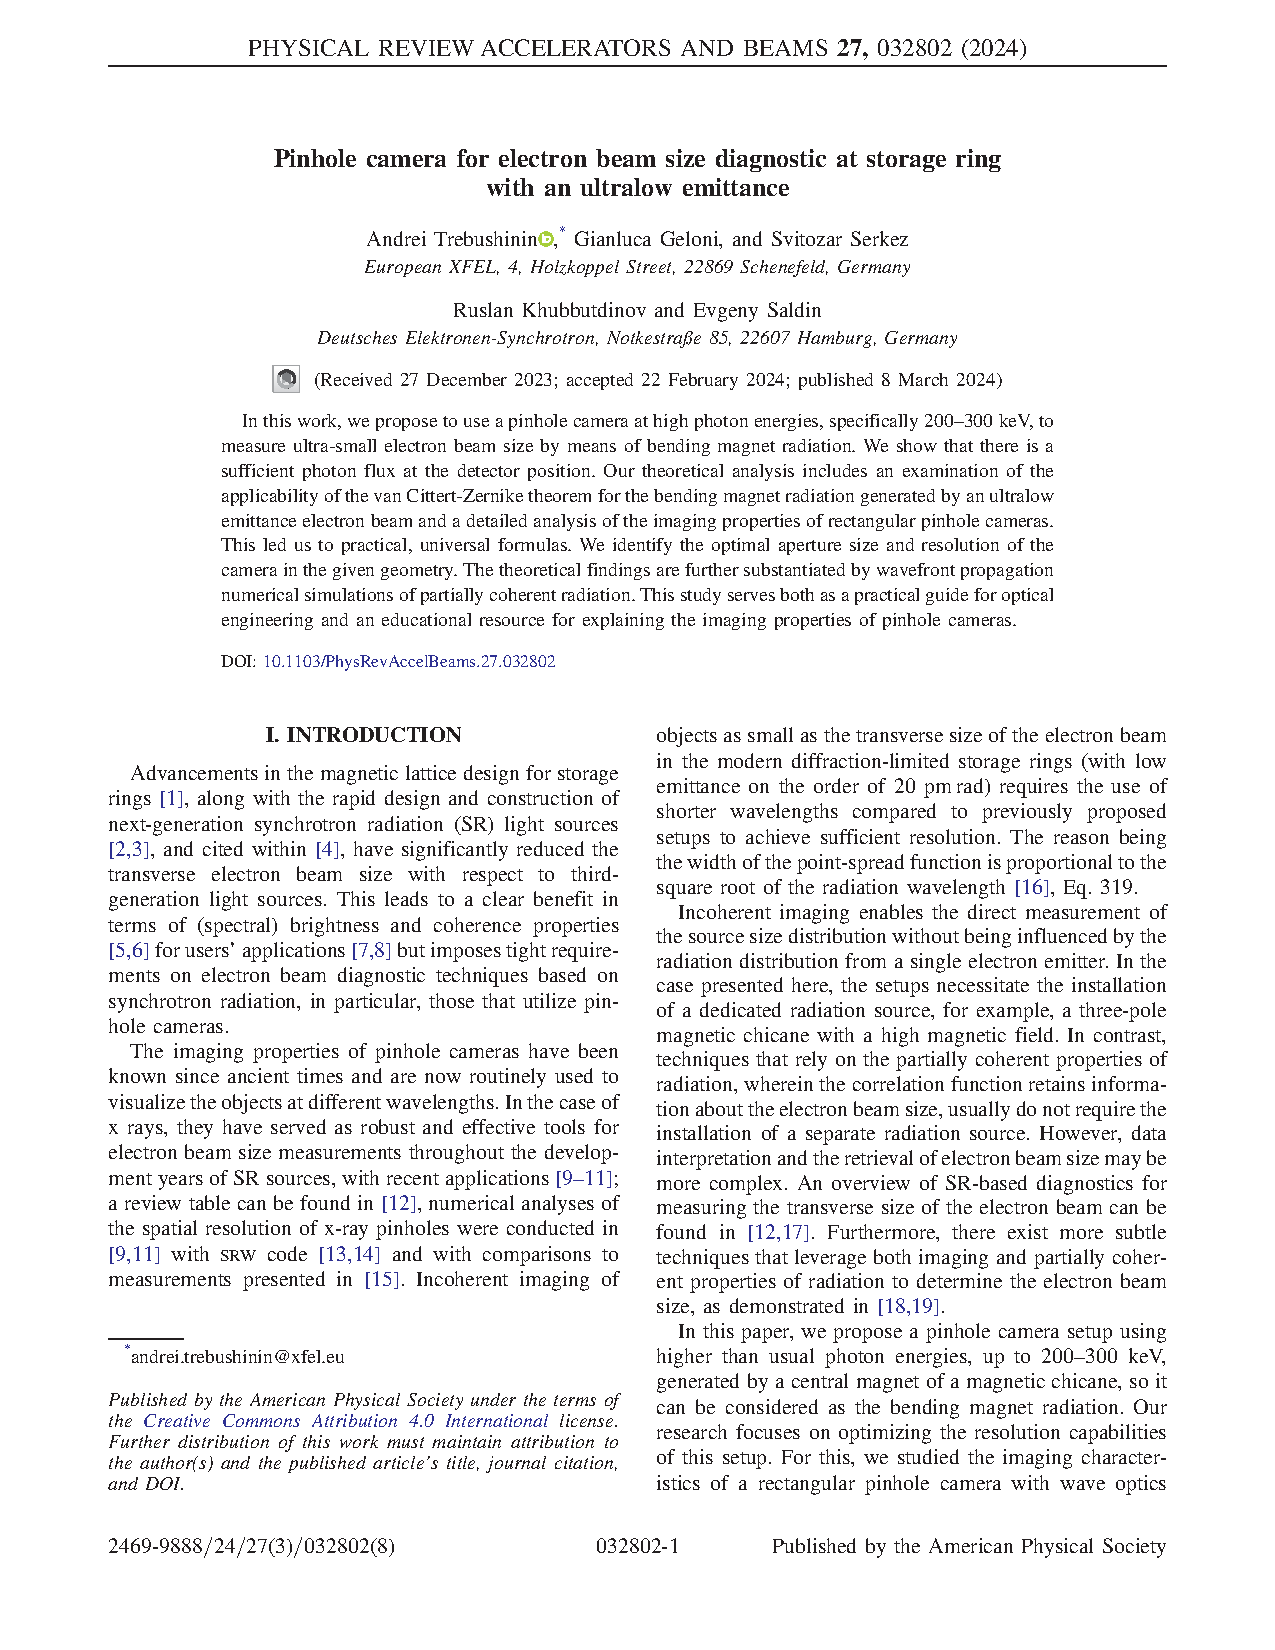
\includepdf[pages=-]{content/papers/pinhole.pdf}

\setcounter{mycounter}{2}
\section{Heuristic approach \Roman{mycounter}: quasi- homogeneous/stationary sources}
\label{Heuristic approach II: quasi- homogeneous/stationary sources}
    In the Section~\ref{sec:Heuristic approach: homogeneous/stationary source}, I have shown a method for simulating fully incoherent sources. In this section, I would like to extend these algorithms to account for finite source divergence. As will become clear from the derivation, confining the divergence of a source will inevitably result in an increased coherence length. Moreover, the resulting field will follow the correct correlation function.
    
    I take the previous Eq.~\ref{Eq:SERVAL0} and the make a Fourier transform of it to the inverce domain:
    \begin{align}
        \bar{\phi}(\vec{k}) = \mathcal{F} \big[ \sqrt{I(\vec{r})} \mathcal{N}(\vec{r})\big](\vec{k})
    \end{align}
    where Fourier transform is denoted as $\mathcal{F} \big[…\big]$ operator. Then I multiply this field by the effective radiation divergence at the source location $\hat{I}(\vec{k})$ and take inverse Fourier transform back the real space:
    \begin{align}
        \phi(\vec{r}) = \mathcal{F}^{-1} \bigg[ \sqrt{\hat{I}(\vec{k})} \mathcal{F} \big[ \sqrt{I(\vec{r})} \mathcal{N}(\vec{r})\big](\vec{k})\bigg](\vec{r}).
        \label{Eq:SERVAL1}
    \end{align}
    Again the hypothesis is that the field in Eq.~\ref{Eq:SERVAL1} follows correct correlation function. To check this I perform auto-correlation and write the integrals of the direct Fourier transform explicitly:
    \begin{align}
        \langle \phi(\vec{r}_1) \phi^*(\vec{r}_2) \rangle =  
        \mathcal{F}^{-1} \bigg[  \sqrt{\hat{I}(\vec{k}_1)\hat{I}(\vec{k}_2)} \iint \limits_{-\infty}^{\infty}  \sqrt{I(\vec{r}'_1)I(\vec{r}'_1)} \big \langle\mathcal{N}(\vec{r}'_1)\mathcal{N}(\vec{r}'_2) \big \rangle e^{i (\vec{r}'_1\vec{k}_1 - \vec{r}'_2\vec{k}_2)}d\vec{r}'_1 d\vec{r}'_2  \bigg](\vec{r}_1, \vec{r}_2),
    \end{align}
    where I bring the averaging sign under the integral sign and accounting for the noise property: $\langle \mathcal{N}(\vec{r}_1)\mathcal{N}^*(\vec{r}_2)\rangle = \delta(\vec{r}_2 - \vec{r}_1)$ I result in the following expression:
    \begin{align}
        \langle \phi(\vec{r}_1) \phi^*(\vec{r}_2) \rangle =  
        \mathcal{F}^{-1} \bigg[  \sqrt{\hat{I}(\vec{k}_1)\hat{I}(\vec{k}_2)}  \iint \limits_{-\infty}^{\infty}  \sqrt{I(\vec{r}'_1)I(\vec{r}'_1)} \delta(\vec{r}'_1 - \vec{r}'_2) e^{i (\vec{r}'_1\vec{k}_1 - \vec{r}'_2\vec{k}_2)}d\vec{r}'_1 d\vec{r}'_2 \bigg](\vec{r}_1, \vec{r}_2).
    \end{align}
    After this I integrate over $d\vec{r}_1$ accounting for the filtering property of Dirac delta function and obtain:
    \begin{align}
        \langle \phi(\vec{r}_1) \phi^*(\vec{r}_2) \rangle =  
        \mathcal{F}^{-1} \bigg[ \sqrt{\hat{I}(\vec{k}_1)\hat{I}(\vec{k}_2)} \int \limits_{-\infty}^{\infty}  I(\vec{r}') e^{i (\vec{r}'(\vec{k}_1 - \vec{k}_2)}d\vec{r}'  \bigg](\vec{r}_1, \vec{r}_2).
    \end{align}
    The explicitly written integral in this expression contains another integral that resembles one from the generalized van Cittert-Zernike theorem. So, changing this to $\hat{g}(\Delta \vec{k})$:
    \begin{align}
        \langle \phi(\vec{r}_1) \phi^*(\vec{r}_2) \rangle =  
        \iint \limits_{-\infty}^{\infty}  \sqrt{\hat{I}(\vec{k}_1)\hat{I}(\vec{k}_2)}\hat{g}(\Delta \vec{k}) e^{-i (\vec{r}_1\vec{k}_1 - \vec{r}_2\vec{k}_2)} d\vec{k}_1 d\vec{k}_2.
    \end{align}
    Then changing $\sqrt{\hat{I}(\vec{k}_1)\hat{I}(\vec{k}_2)}\hat{g}(\Delta \vec{k})$ by $\langle \hat{E}(\vec{k}_1) \hat{E}^{*}(\vec{k}_2) \rangle$ following the general definition of quasi-homogeneity in Eq.~\ref{Eq:quasi_homogeneous_source_weak}. Then, I result in the following expressions:
    \begin{align}
        \langle \phi(\vec{r}_1) \phi^*(\vec{r}_2) \rangle = \cr 
        = \iint \limits_{-\infty}^{\infty} \langle \hat{E}(\vec{k}_1) \hat{E}^{*}(\vec{k}_2) \rangle  e^{-i (\vec{r}_1\vec{k}_1 - \vec{r}_2\vec{k}_2)} d\vec{k}_1 d\vec{k}_2 = \cr
        = \bigg\langle \int \limits_{-\infty}^{\infty} \hat{E}(\vec{k}_1) e^{-i \vec{r}_1\vec{k}_1} d\vec{k}_1 \int \limits_{-\infty}^{\infty} \hat{E}^{*}(\vec{k}_2) e^{i \vec{r}_2\vec{k}_2} d\vec{k}_2 \bigg\rangle = \langle E(\vec{r}_1)E^{*}(\vec{r}_2) \rangle.
    \end{align}
    I have derived that the field $\phi(\vec{r})$ follows the same correlation function as the field $E(\vec{r})$. Since we are working with Gaussian random processes, higher-order correlation functions can be expressed in terms of the first-order correlation function.

    \rr{actually it would be very nice to show that power distribution follow negative exponent.}
    
    In Paper II, I discuss the implementation of this algorithm in the context of undulator radiation. It is important to note that the variables in the algorithm can be exchanged for longitudinal ones, yielding the same results. This equivalence highlights the mathematical similarity between the van Cittert-Zernike theorem and the Wiener-Khinchin theorem. For instance, this algorithm can be used to simulate the longitudinal domain of chirp-free SASE radiation from a free-electron laser (FEL).

    \rr{again write some more}
    
\newpage    
\setcounter{mycounter}{2} % Set the counter to 1
\section{Paper \Roman{mycounter}}

    In the paper by A. Trebushinin, G. Geloni, Y. Rakshun, and S. Serkez, Gaussian Random Field Generator for Simulating Partially Coherent Undulator Radiation, Optica 9, 842 (2022),
    we introduced a computationally efficient algorithm to simulate partially coherent synchrotron radiation fields from undulators, specifically tailored for applications in modern synchrotron radiation sources with low electron beam emittance. This simulation addresses the stochastic nature of radiation fields that arise from shot noise in electron beams, an aspect often simplified and discarded in synchrotron radiation simulations.
    
    The proposed method, referred to as the Synchrotron Emission Rapid eVALuator (SERVAL), utilizes Gaussian random fields to generate statistical realizations of the radiation field at a given frequency. This technique allows to shape a complex amplitude by constraining complex Gaussian noise by the effective size and divergence of the radiation field as have been described in Sec.~\ref{Heuristic approach II: quasi- homogeneous/stationary sources}. This algorithm significantly speeds up the calculations compared to traditional Monte Carlo-like approaches. As a result, we obtain undulator radiation fields that encompass all coherent modes at once if we think of the result in terms of coherent mode decomposition methods.
    
    We provide a detailed theoretical background on the statistical properties of undulator radiation, highlighting the intrinsic stochastic structure due to the random distribution of electrons within the beam. They illustrate how our approach is consistent with established theoretical frameworks and offers computational algorithms. The method has been validated against other simulation approaches, demonstrating its effectiveness in capturing the statistical properties of synchrotron radiation.
    
    Practically, SERVAL capabilities are demonstrated through simulations that involve typical components of synchrotron beamlines, such as focusing systems. These demonstrations show how the method can be integrated into existing simulation frameworks like Ocelot~\cite{ocelot-collab_ocelot_2017} for comprehensive start-to-end modeling of radiation at synchrotron facilities. In summary, this paper presents an advancement in the simulation of synchrotron radiation, offering a fast and accurate method to model the partially coherent radiation produced by undulators. We believe that this approach not only enhances the design and optimization of synchrotron light sources but also serves as an educational tool for understanding complex radiation phenomena.

\includepdf[pages=-]{content/papers/SERVAL.pdf}
\section{Coherence properties of SASE FEL radiation}
    In this section, I will briefly discuss the coherence properties of SASE FEL. Comprehensive presentations on the statistical properties of SASE FEL can be found in pioneering works~\cite{saldin_statistical_1998} and in textbooks on FEL physics. Here, I will outline the fundamental aspects needed for the further development of the SERVAL algorithm. I will focus on the longitudinal coherence properties of SASE radiation, assuming that the radiation is fully coherent transversely. I will revisit this point at the conclusion of this chapter.

    \rr{this difficult to read, improve this}
    
    The theory previously outlined in this thesis encapsulates the statistical properties of Gaussian processes and is applicable to more complex processes like SASE, albeit with some limitations. SASE amplification, despite its laser-like name, starts from usual synchrotron radiation. Up to the moment of saturation\footnote{The term refers to the phase where there is an exponential gain in the power of radiation.}, Gaussian statistics are preserved. This regime of operation is called the linear regime, which refers to the exponential gain in the power of radiation. The term "linear" is used in reference to electric circuits amplifiers. Only after reaching saturation the radiation statistics start to deviate from Gaussian statistics, as described in~\cite{saldin_statistical_1998}. Therefore, for developing SERVAL, it means that up to the moment of saturation, one can apply SERVAL-like algorithms. For illustration, I plot the evolution of the SASE process in Fig.~\ref{Fig:evo_spikes} in addition to this, a more detailed explanation on SASE process within this thesis can be found in Paper IV,~\cite{trebushinin_experimental_2023}.
    \begin{figure*}[h!]
    	\centering
        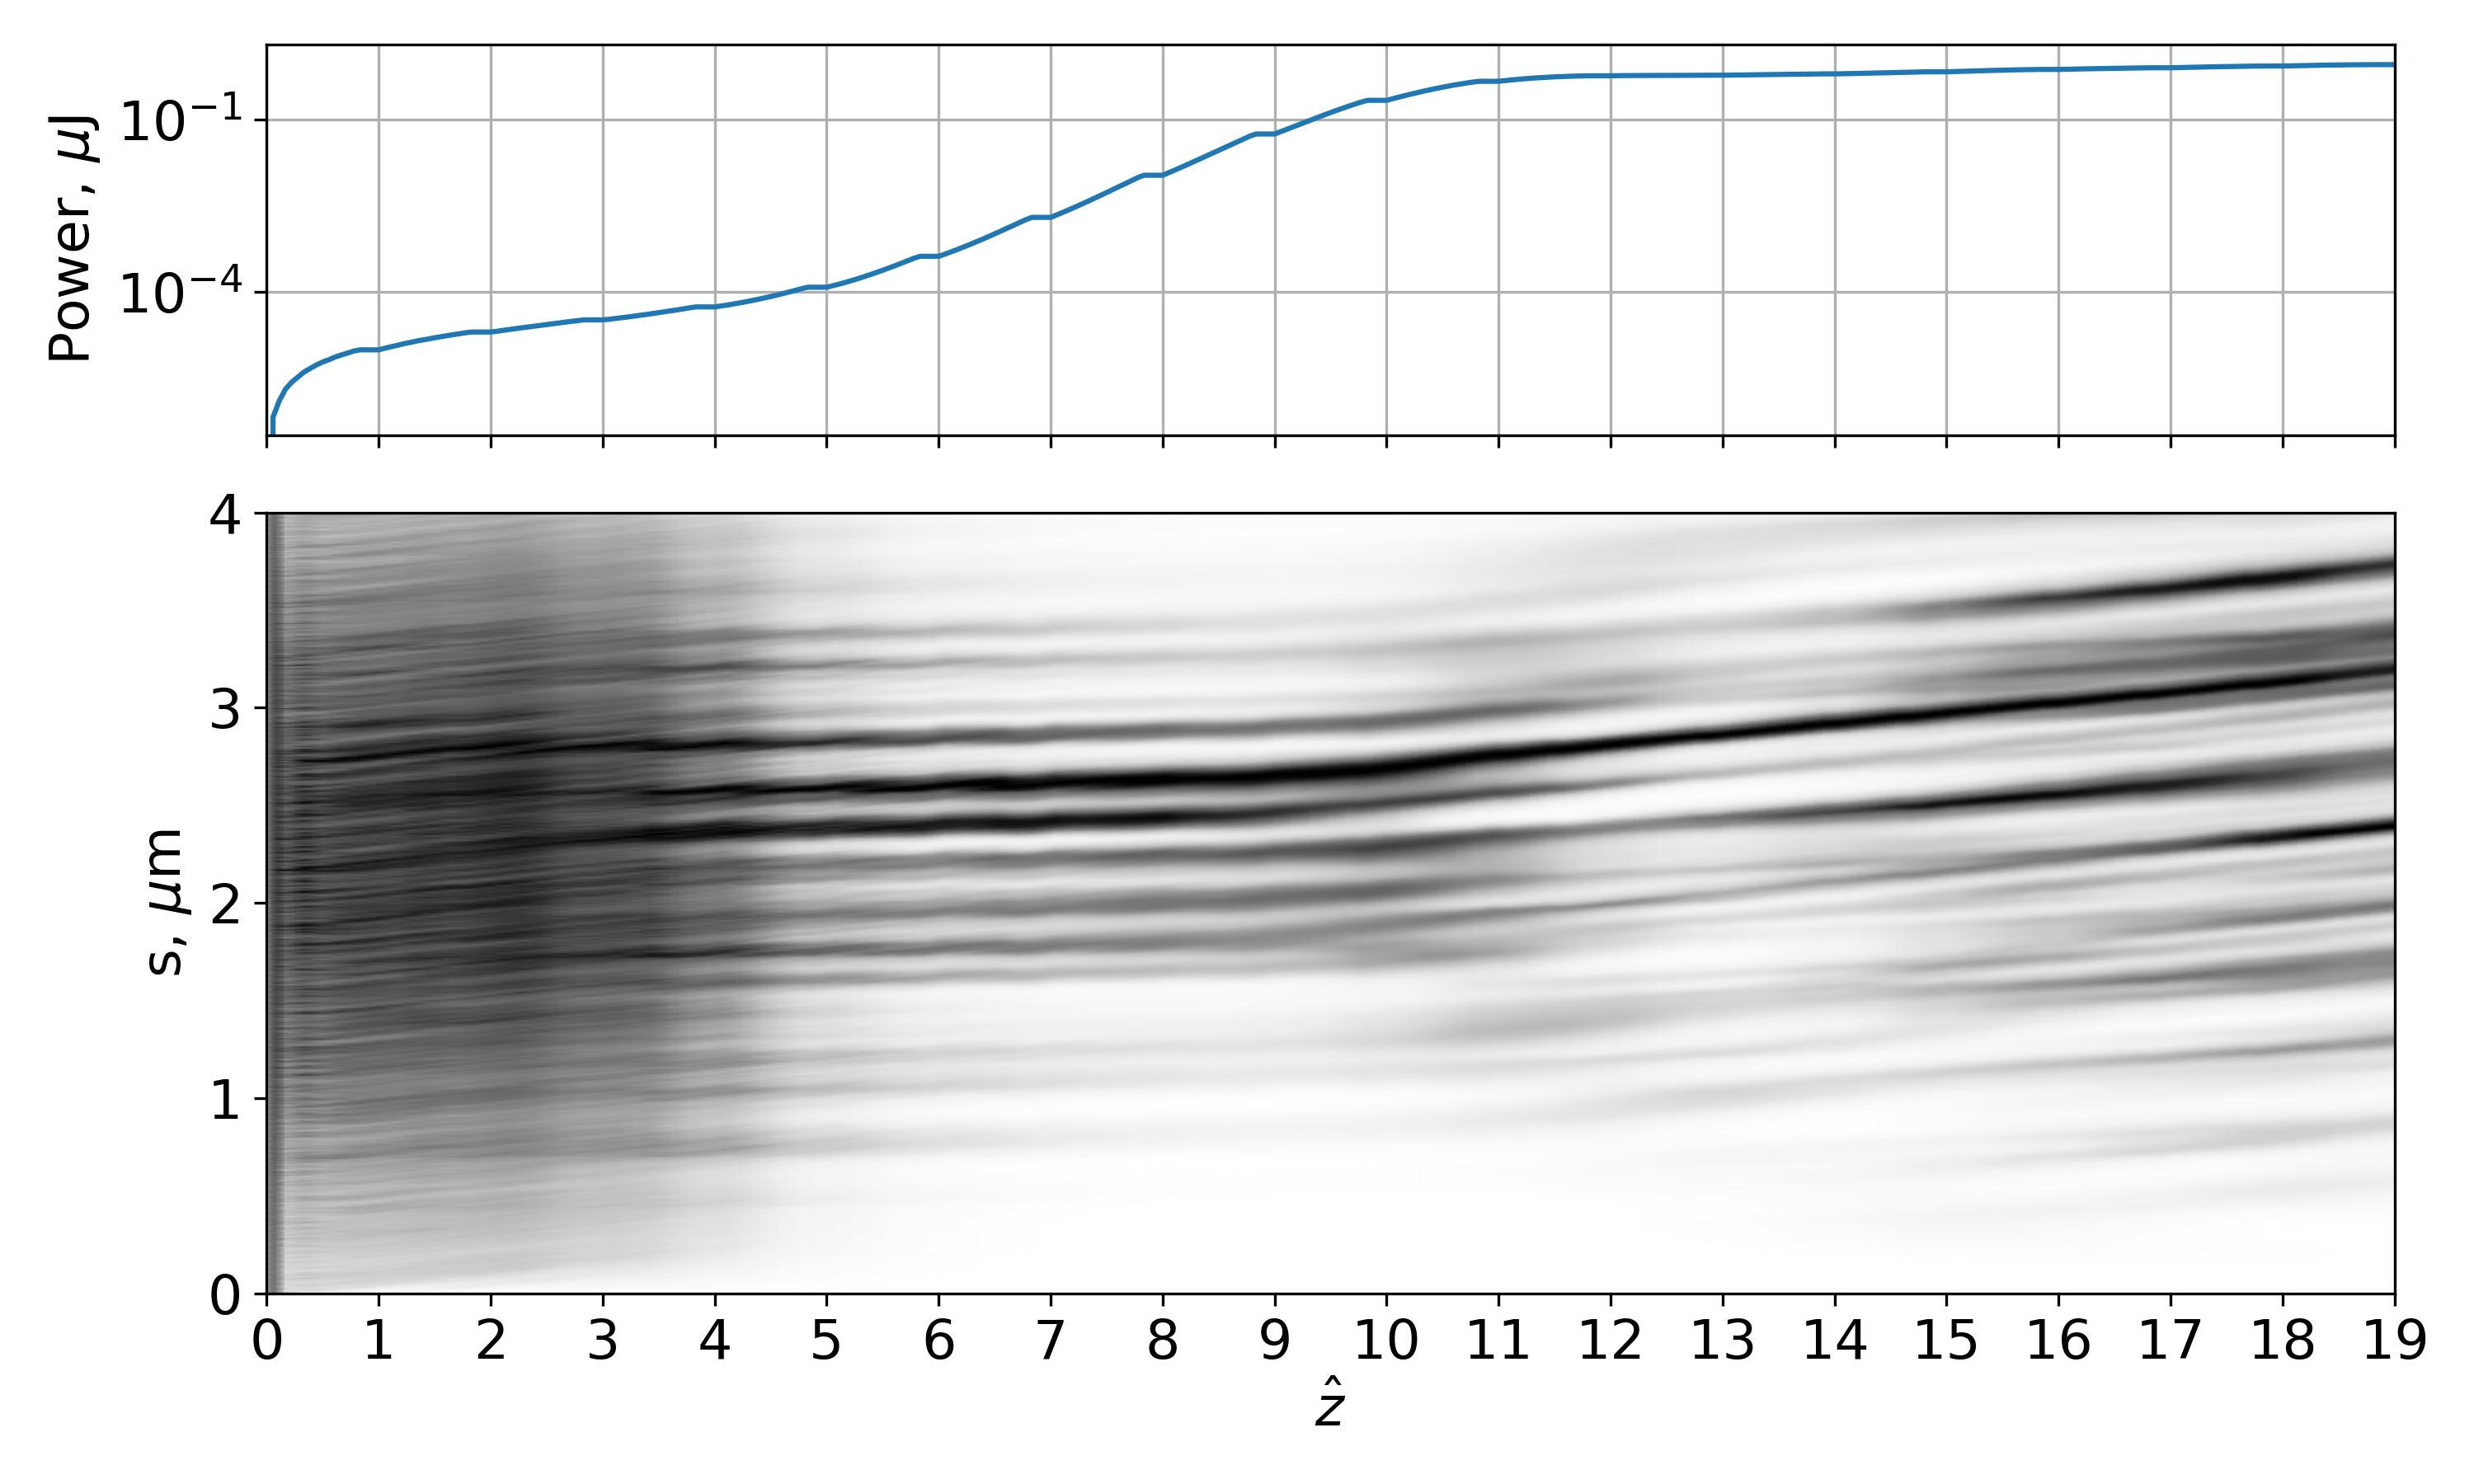
\includegraphics[width=0.95\linewidth]{content/images/4_FEL_Theory/evo_spikes.png}
    \captionsetup{justification=centering}
        \caption{SASE lasing process: Radiation starts from shot noise and is steadily amplified exponentially until reaching saturation around $\hat{z} = 10$, after which the radiation power grows nearly linearly.}
        \label{Fig:evo_spikes}
    \end{figure*}
    
    Transversely, radiation undergoes a mode selection process and rapidly acquires almost full transverse coherence. I illustrate this in Fig.~\ref{Fig:transverse_modes}:
    \begin{figure*}[h!]
    	\centering
        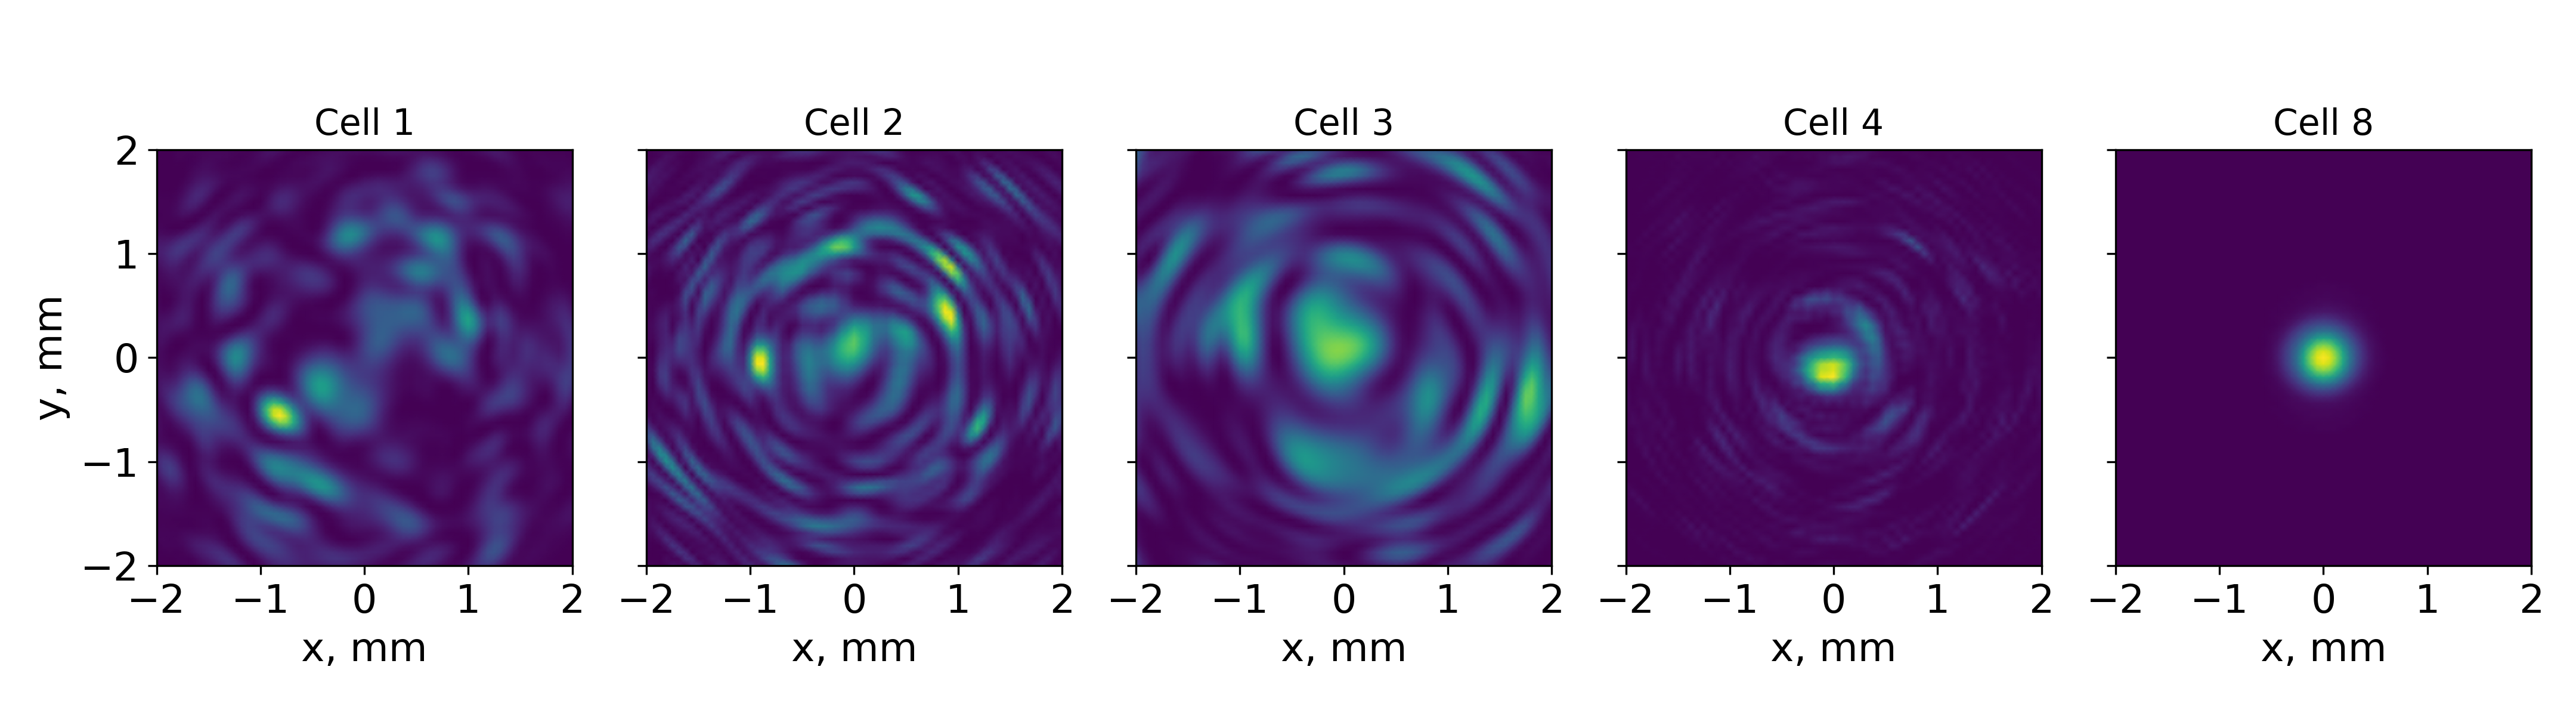
\includegraphics[width=0.99\linewidth]{content/images/4_FEL_Theory/transverse_modes.png}
        \captionsetup{justification=centering}
        \caption{Transverse intensity distribution of monochromatized radiation view in the far zone from the number of cell labeled on top of sub figure.}
        \label{Fig:transverse_modes}
    \end{figure*} 
    From here on, I assume that SASE radiation is in a transversely coherent state, and I focus on describing the longitudinal domain of the SASE radiation, as it is of the most interest for practical cases.

    Radiation properties in the longitudinal (time-frequency) domain heavily depend on the energy chirp in the electron beam. It can be easily shown with the undulator resonance condition that the energy chirp of the electron beam relates to the radiation frequency as follows:
    \begin{align}
        \omega(t) = \frac{2 \gamma^2(t)k_w c}{1 + K^2/2},
    \end{align}
    where $\gamma(t) = \gamma_0 + \gamma_n(t)$. Normally the value of energy variation $\gamma_n(t)$ is so small (i.e. $\gamma_n(t)/\gamma_0 \ll 1$) that one can expand $\gamma^2(t)$ and obtain the following expression:
    \begin{align}
        \omega(t) = \frac{2\gamma_0^2k_w c}{1 + K^2/2}\bigg(1 + 2\frac{\gamma_n(t)}{\gamma_0}\bigg) 
    \end{align}
    As one can see here, in the first approximation, SASE radiation's instantaneous frequency replicates the chirp in the electron beam. Now, it is time to examine the phase space of such radiation.
    
    One way to represent the structure of the radiation phase is through the Wigner distribution, which I define as follows:
    \begin{align}
        \mathcal{W}(\bar{t}, \bar{\omega}) = \int \limits_{-\infty}^{\infty} \Tilde{\Gamma}(\bar{\omega}, \Delta \omega) e^{-i\Delta \omega \bar{t}}d(\Delta \omega)
    \end{align}

    Having this, one can represent the radiation distribution in the space of the time-domain (longitudinal coordinate along the beam) and frequency (photon energy). Moreover, one can represent a single statistical realization in terms of the Wigner function distribution. This can be done based on the fact that the averaging operation for $\Tilde{\Gamma}(\bar{\omega}, \Delta \omega)$ can be taken out of the integral, i.e., taking the integral and averaging can be exchanged in order. In this way, a Wigner function of a single realization makes sense, as well as averaging single-shot Wigner functions to obtain an averaged one.
    
    In Fig.~\ref{Fig:ROSA_linear_chirp}, I present such a Wigner function from a single realization of SASE radiation from a linearly chirped electron beam. With this figure, I introduce important concepts such as instantaneous bandwidth, instantaneous frequency, group delay, and group duration, which are outlined in Fig.~\ref{Fig:ROSA_linear_chirp} and are hopefully self-explanatory. 
    \begin{figure}[h!]
    	\centering
        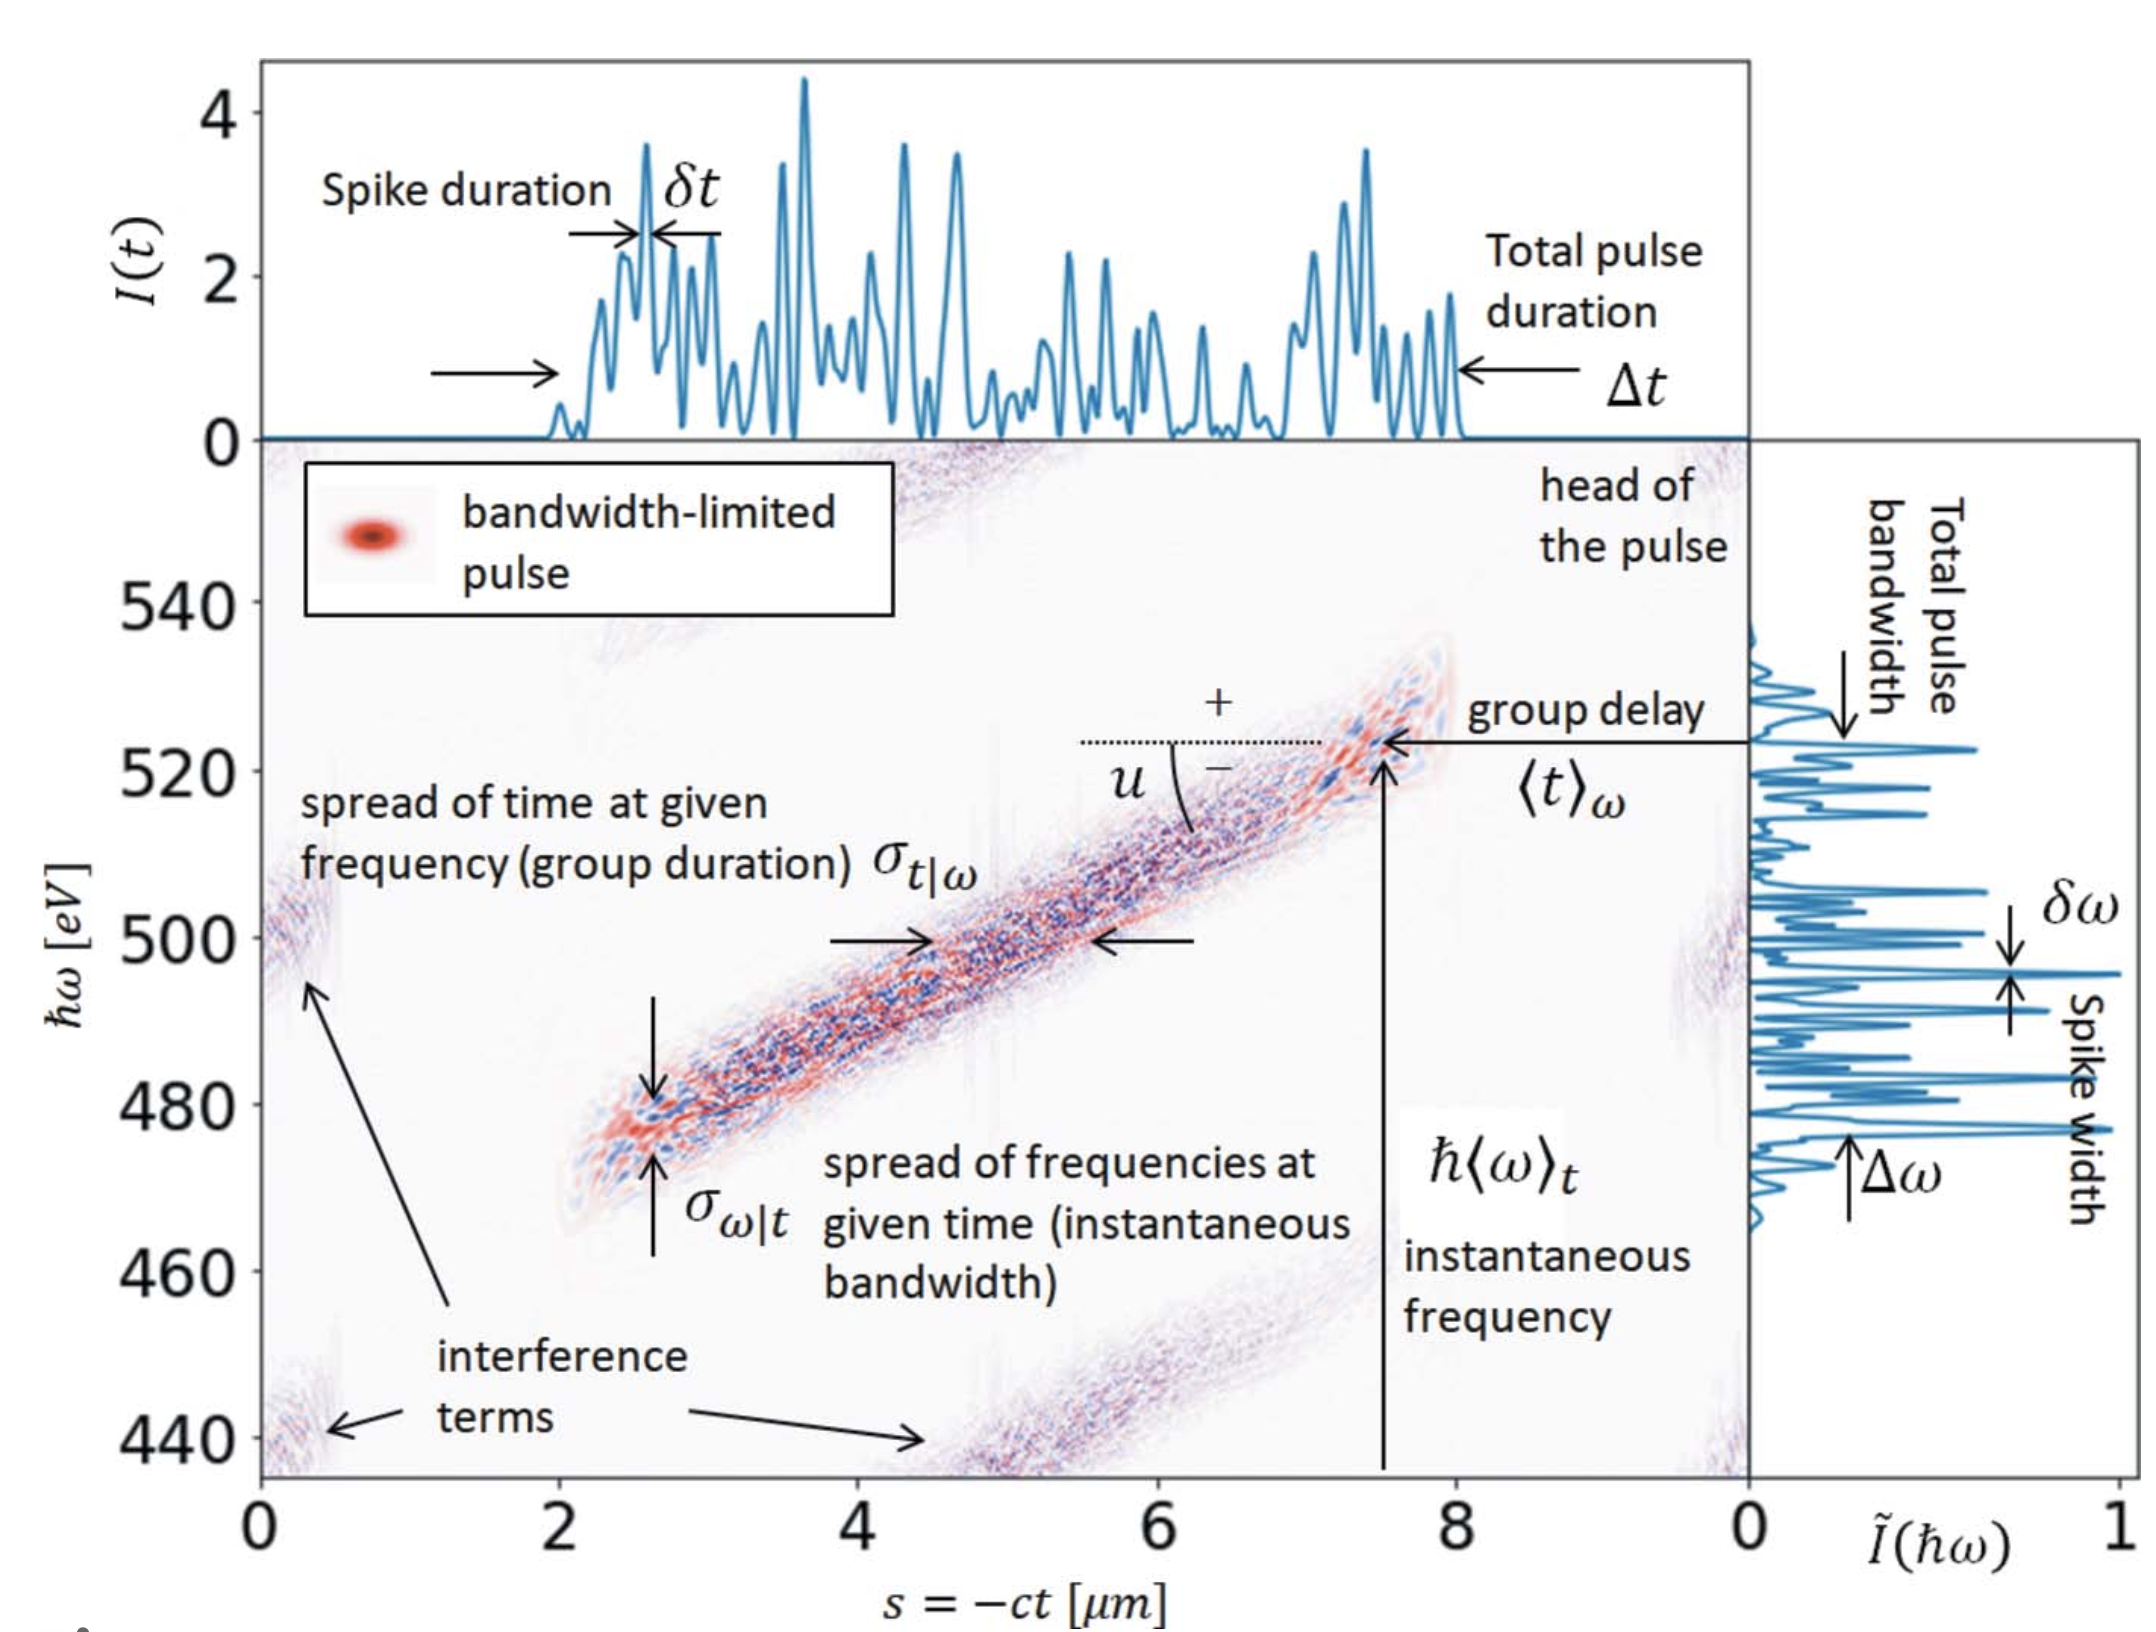
\includegraphics[width=0.75\linewidth]{content/images/4_FEL_Theory/ROSA_linear_chirp.png}
        \captionsetup{justification=centering}
        \caption{\textbf{Adopted from \cite{serkez_wigner_2021}} The European XFEL 100 pC electron beam with a non-linear energy chirp produces SASE radiation with different durations at different photon energies. Note the bifurcation in Wigner distribution above 499 eV. Analysis based on 1000 simulated SASE spectra.}
        \label{Fig:ROSA_linear_chirp}
    \end{figure} 
    In real experiments at facilities such as the European XFEL, electron beams often exhibit nonlinear frequency chirps~\rr{cite}. A simulation of one such example is presented in Fig.~\ref{Fig:ROSA_sim}. Simulating these distributions aims to reproduce results from the real experiment and validate the ROSA algorithms~\cite{serkez_wigner_2021}.
    \begin{figure}[h!]
    	\centering
        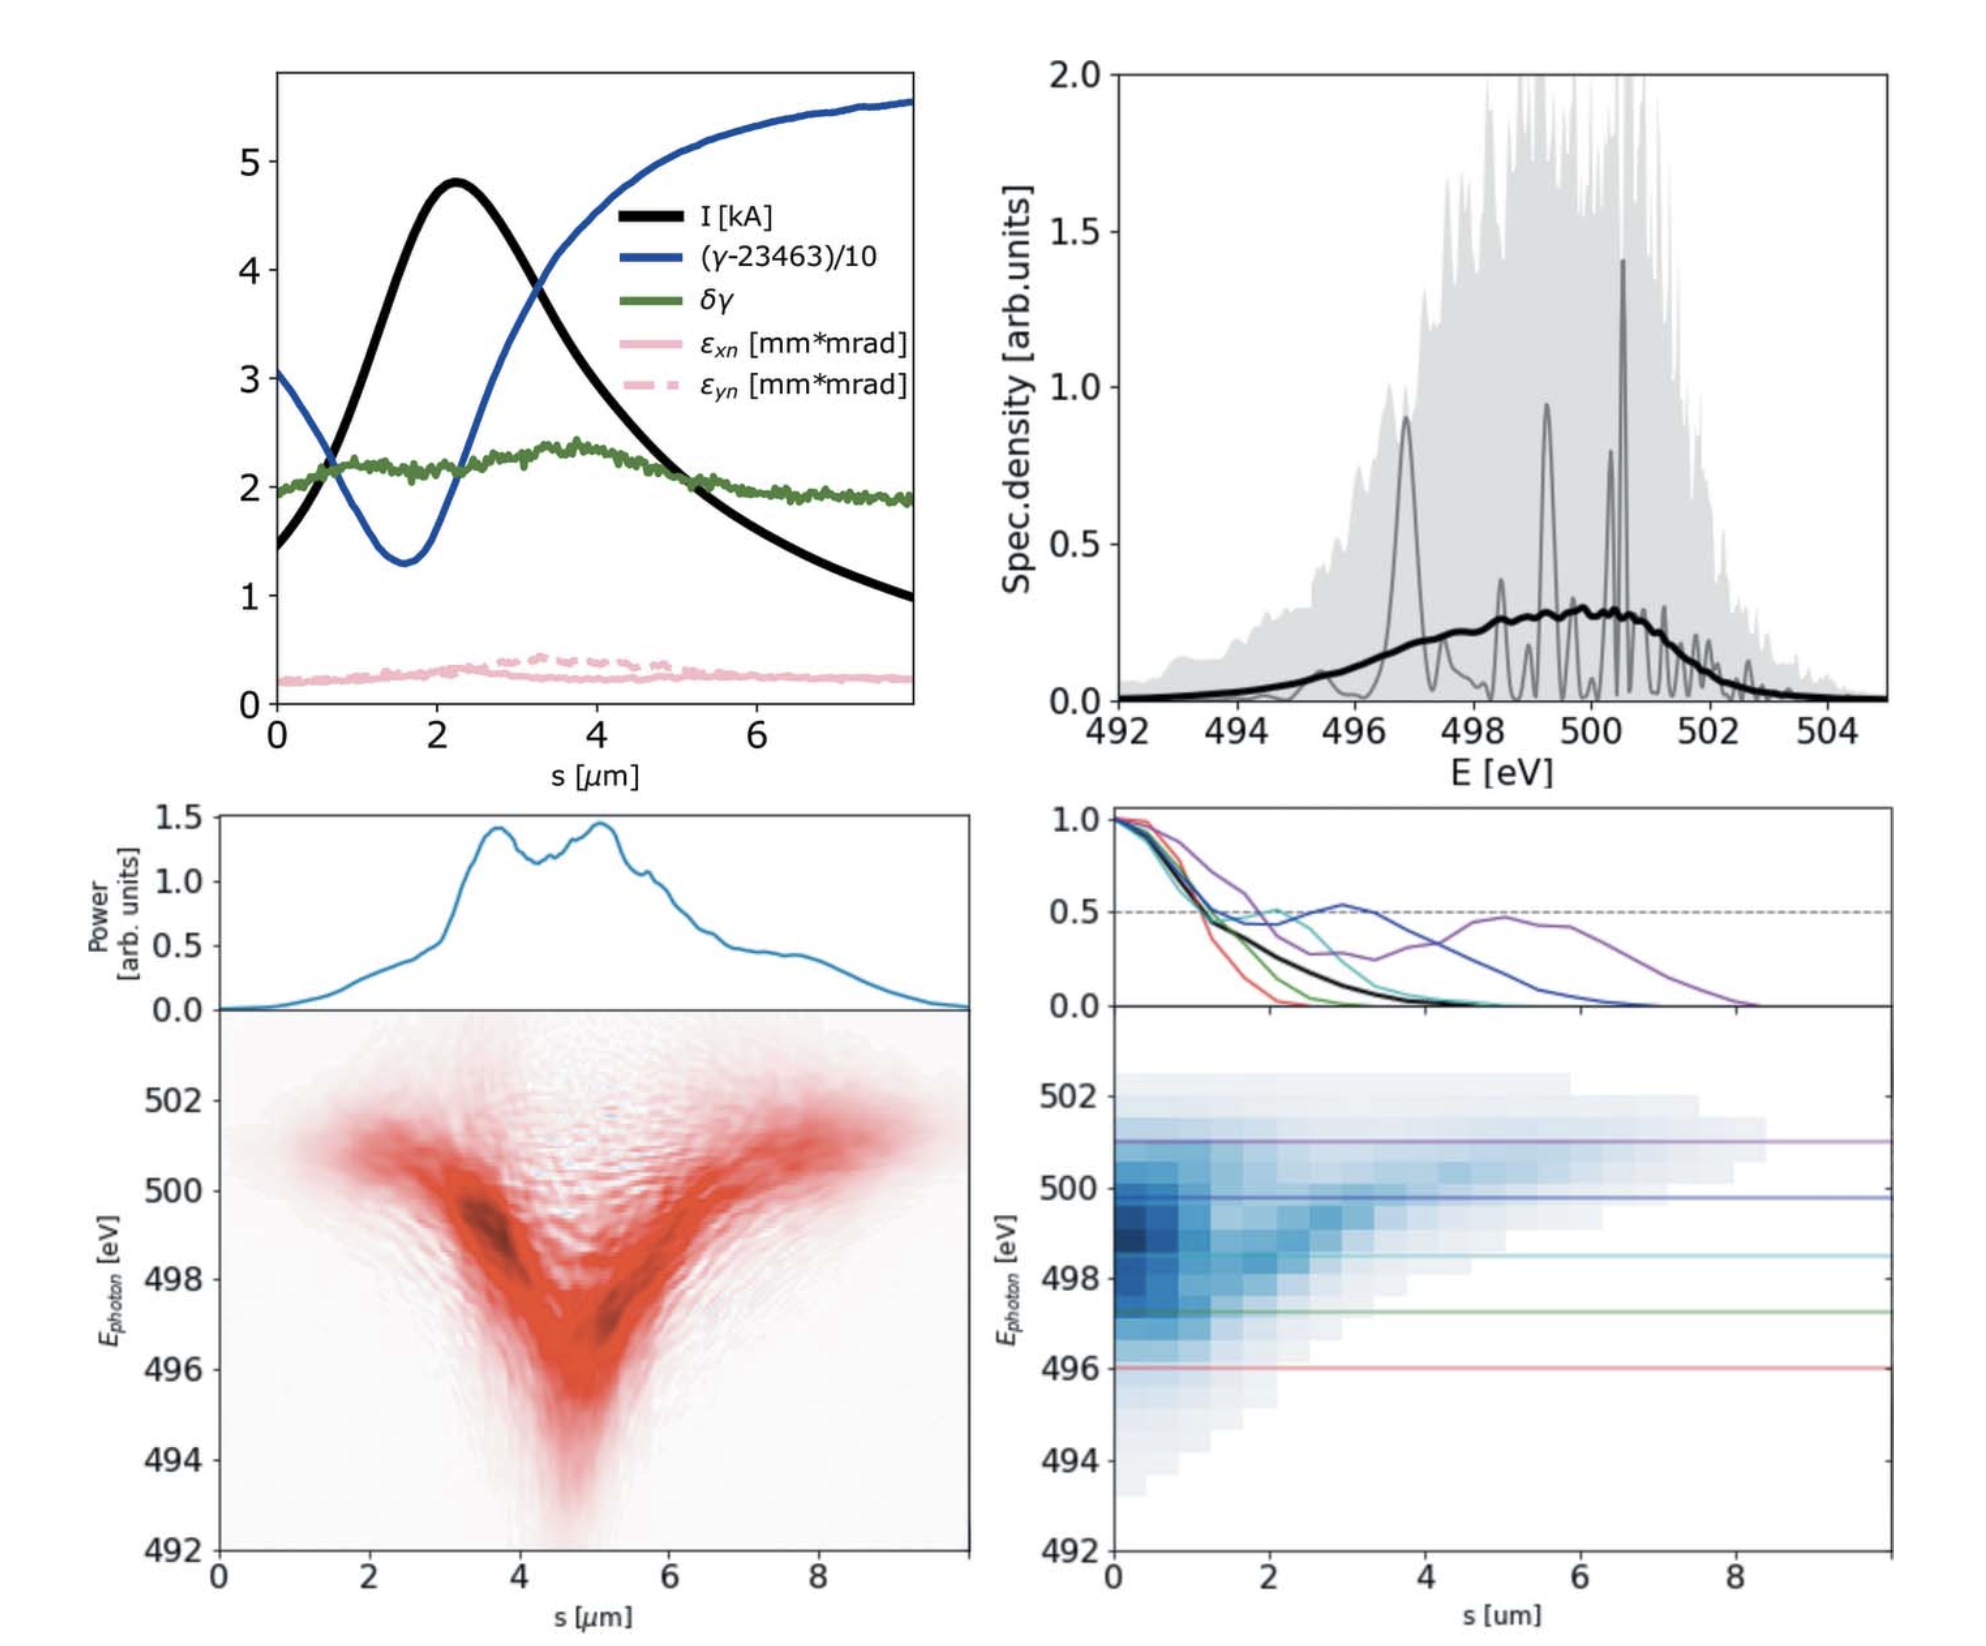
\includegraphics[width=0.75
        \linewidth]{content/images/4_FEL_Theory/ROSA_sim.png}
        \captionsetup{justification=centering}
        \caption{\textbf{Adopted from \cite{serkez_wigner_2021}}}
        \label{Fig:ROSA_sim}
    \end{figure} 
    The next goal for developing the SERVAL algorithm is to enable it to account for these kinds of frequency chirps or, more generally, arbitrary Wigner function distributions of the radiation. The results of this activity are presented in the subsequent section and in Paper IV.

\setcounter{mycounter}{3}
\section{Heuristic approach \Roman{mycounter}: non- homogeneous / stationary sources}

    One may notice that for a source that can be represented $\Tilde{\Gamma}(\omega, \Delta \omega) = f_{\omega}(\Delta \omega)\bar{I}(\bar{\omega})$ it is possible to take the intensity out under the integral sign, so Wigner function $\mathcal{W}(t, \omega)$ can be written as the following:
    \begin{align}
        \mathcal{W}(\bar{t}, \bar{\omega}) = \bar{I}(\bar{\omega}) \int \limits_{-\infty}^{\infty} f_{\omega}(\Delta \omega) e^{-i\Delta \omega \bar{t}}d(\Delta \omega) = \bar{I}(\bar{\omega}) I(\bar{t}).
    \end{align}
    Looking at this expression and \textit{mentally}\footnote{I mention here again that throughout this chapter, I present the algorithms in different pairs of domains — spatial-inverse spatial and time-frequency domains. This is justified by the fact that the van Cittert-Zernike theorem for the transverse domain and the Wiener-Khinchin theorem for the longitudinal domain are similar relations, i.e., both are based on Fourier transforms. Thus, I use the same algorithms for these pairs of domains almost without changes.} changing the variables to transverse ones, it is clear that in the previous version of SERVAL in Eq.~\ref{Eq:SERVAL1}, I implicitly used the factorized Wigner function.
    
    Now instead of factorising the Wigner function, I write it as it is under the first integral:
    \begin{align}
    	\phi(\bar{\omega}) = \int \limits_{-\infty}^{\infty} \sqrt{\mathcal{W}(\bar{\omega}, \bar{t})} \mathcal{N}(\bar{t}) e^{i \bar{\omega} \bar{t}} d\bar{t}.
    	\label{Eq:Field_Wigner}
    \end{align}
    My hypothesis is the following: Eq.~\ref{Eq:Field_Wigner} can indeed represent a real field that has the correlation function $\Tilde{\Gamma}(\omega, \Delta \omega)$. This I will study the following Paper III.
    
\newpage    
\setcounter{mycounter}{3} % Set the counter to 1
\section{Paper \Roman{mycounter}}
    
    In the paper A. Trebushinin, G. Geloni, and S. Serkez, Algorithm for modeling partially coherent radiation with an arbitrary Wigner function, we introduce an upgraded algorithm compared to one presented in~\cite{trebushinin_gaussian_2022}. This approach utilizes a Wigner function distribution to accurately model the stochastic properties of radiation fields, which is particularly relevant for advanced radiation sources like synchrotrons and free-electron lasers (FELs).
    
    The algorithm builds on the concept of simulating Gaussian random fields, where noise is generated and then constrained by the effective support in both Fourier domain weather it is time -- frequency one or spatial -- inverse spatial. This method is computationally efficient and allows for the propagation of the simulated field through various optical elements. We verified that the simulated fields adhere to the correct statistical descriptions by comparing ensemble-averaged intensities and correlation functions against theoretical predictions and numerical results. The paper elaborates on several key applications, including simulations of double-slit experiments and SASE radiation from FELs. These examples demonstrate the versatility of the algorithm in handling different types of radiation sources, including those with complex temporal and spatial coherence properties as SASE radiation with different frequency chirps.
    
    We also discuss potential extensions of the algorithm, suggesting its applicability to non-Gaussian sources and more complex spatial-temporal coherence scenarios. We argue on the algorithm's flexibility and computational efficiency make it a potent tool for both research and educational purposes in the field of physical and statistical optics. Overall, the paper provides a comprehensive framework for simulating partially coherent radiation, with significant implications for the design and analysis of optical systems and experiments in modern synchrotron and FEL facilities.
    
\includepdf[pages=-]{content/papers/SERVAL2.pdf}


\newpage    
\setcounter{mycounter}{4} % Set the counter to 1
\section{Paper \Roman{mycounter}}
    In the following paper I will present a special mode of SASE FEL operation, demonstrating that the resulting radiation does not adhere to Gaussian statistics. With this example, I aim to illustrate that the application of SERVAL algorithms should always be done thoughtfully, based on the specific case under study. For instance, when it was not possible to use SERVAL, I had to perform simulations using the Genesis 1.3 code.
    
    In the paper A. Trebushinin, G. Geloni, S. Serkez, G. Mercurio, N. Gerasimova, T. Maltezopoulos, M. Guetg, and E. Schneidmiller, Experimental Demonstration of Attoseconds-at-Harmonics at the SASE3 Undulator of the European XFEL, Photonics 10, 2 (2023), we present an experiment generating sub-femtosecond pulses using the 'attosecond-at-harmonic' method at Free Electron Lasers (FELs). The research, conducted at the European XFEL's SASE3 undulator, demonstrated a method to produce short pulses through harmonic conversion, specifically targeting the fourth harmonic.

    The experimental setup involved a two-stage process. In the first stage, the undulator amplified the electron bunching at both the fundamental frequency and higher harmonics. In the second stage, the SASE3 undulator, tuned specifically to the fourth harmonic, further amplified these pulses to achieve shorter durations. Statistically, not all pulses were single-spike events, but we identified that depending on the experimental conditions, 3\% to 13\% of the generated pulses were single-spike events. In the paper, we report the creation of pulses with a lower estimated duration of 650 attoseconds.
    
    The technique described, referred to as the 'attoseconds-at-harmonics' method, utilizes minimal hardware modifications, relying only on variable gap undulator cells to achieve the desired harmonic amplification. This method proved to be versatile in settings with limited hardware at a beamline, offering a way to generate short X-ray pulses suitable for probing fast dynamics in materials science, chemistry, and other fields.
    
    This paper outlines not only the experimental setup and results but also discusses the theoretical background, specifically the process of harmonic conversion. The statistics of this radiation are non-Gaussian due to the nonlinear conversion process, as shown in the paper. Interpreting the spectral width to estimate the resulting pulse duration is complicated because there is no direct relationship between the first-order correlation function and higher-order ones usually applied for pulse duration estimation. In this paper, we developed a simulation-based method to provide a correction factor that helped us resulted in a lower estimate of the pulse duration.
    
\includepdf[pages=-]{content/papers/attoharm.pdf}

\section{Conclusion}

    The content of this chapter is intended to enhance the results of the presented papers and vice versa. The chapter is supported by the necessary theoretical background, including an introduction to types of random processes and a discussion of important classes of sources such as stationary and ergodic sources. I then introduced the concept of Gaussian statistics for random processes, which significantly simplifies the analysis of random processes by linking higher-order correlation functions with the first-order one. Following this, I explored concepts such as quasi-stationarity and homogeneity, highlighting their mathematical similarities. Concluding the theoretical part, I outlined coherence theory for synchrotron radiation sources and free-electron lasers.

    \rr{It sounds sketchy, work on this more}
    
    The goal of this chapter is to present three algorithms for simulating fully incoherent fields, partially coherent fields, and partially coherent fields with arbitrary Wigner function distributions. These algorithms replicate  random fields by generating complex Gaussian noise and then constraining this noise with appropriate mathematical supports. For fully incoherent sources, the support is simply the random source intensity distribution. For partially coherent sources, this support is supplemented by the source's effective divergence in the inverse space domain. These approaches assume that the radiation phase space is factorized. However, the algorithm can be extended to simulate fields with arbitrary phase space distributions using the Wigner function. All three algorithms have practical applications, such as simulating bending magnet radiation, undulator radiation, and FEL SASE radiation in the linear regime. Additionally, I provided an interesting example of simulating the original Young's double slit experiment using one of the versions of the code. I have endeavored to explain not only the practical advancements of these algorithms but also their limitations, which are crucial to consider when simulating complex systems. For example, I mentioned a method that could potentially extend the applicability of these algorithms to non-Gaussian statistics, which could be a subject for further study beyond the scope of this thesis. In conclusion, I hope that the algorithms presented here will serve as valuable tools for optical simulations. Meanwhile, in the next chapter, I will present the result of the experiments for measuring electron beam size at hard X-ray beamlies of European XFEL where SERVAL played very important role at the stage of numerical simulations.

%\chapter{FEL theory: statistical optics perspective}
\label{chapter:FEL theory}


A free-electron laser can be generally considered as an amplifier and its coherence properties can be characterized from this point of view. 

\begin{figure*}[h!]
	\centering
    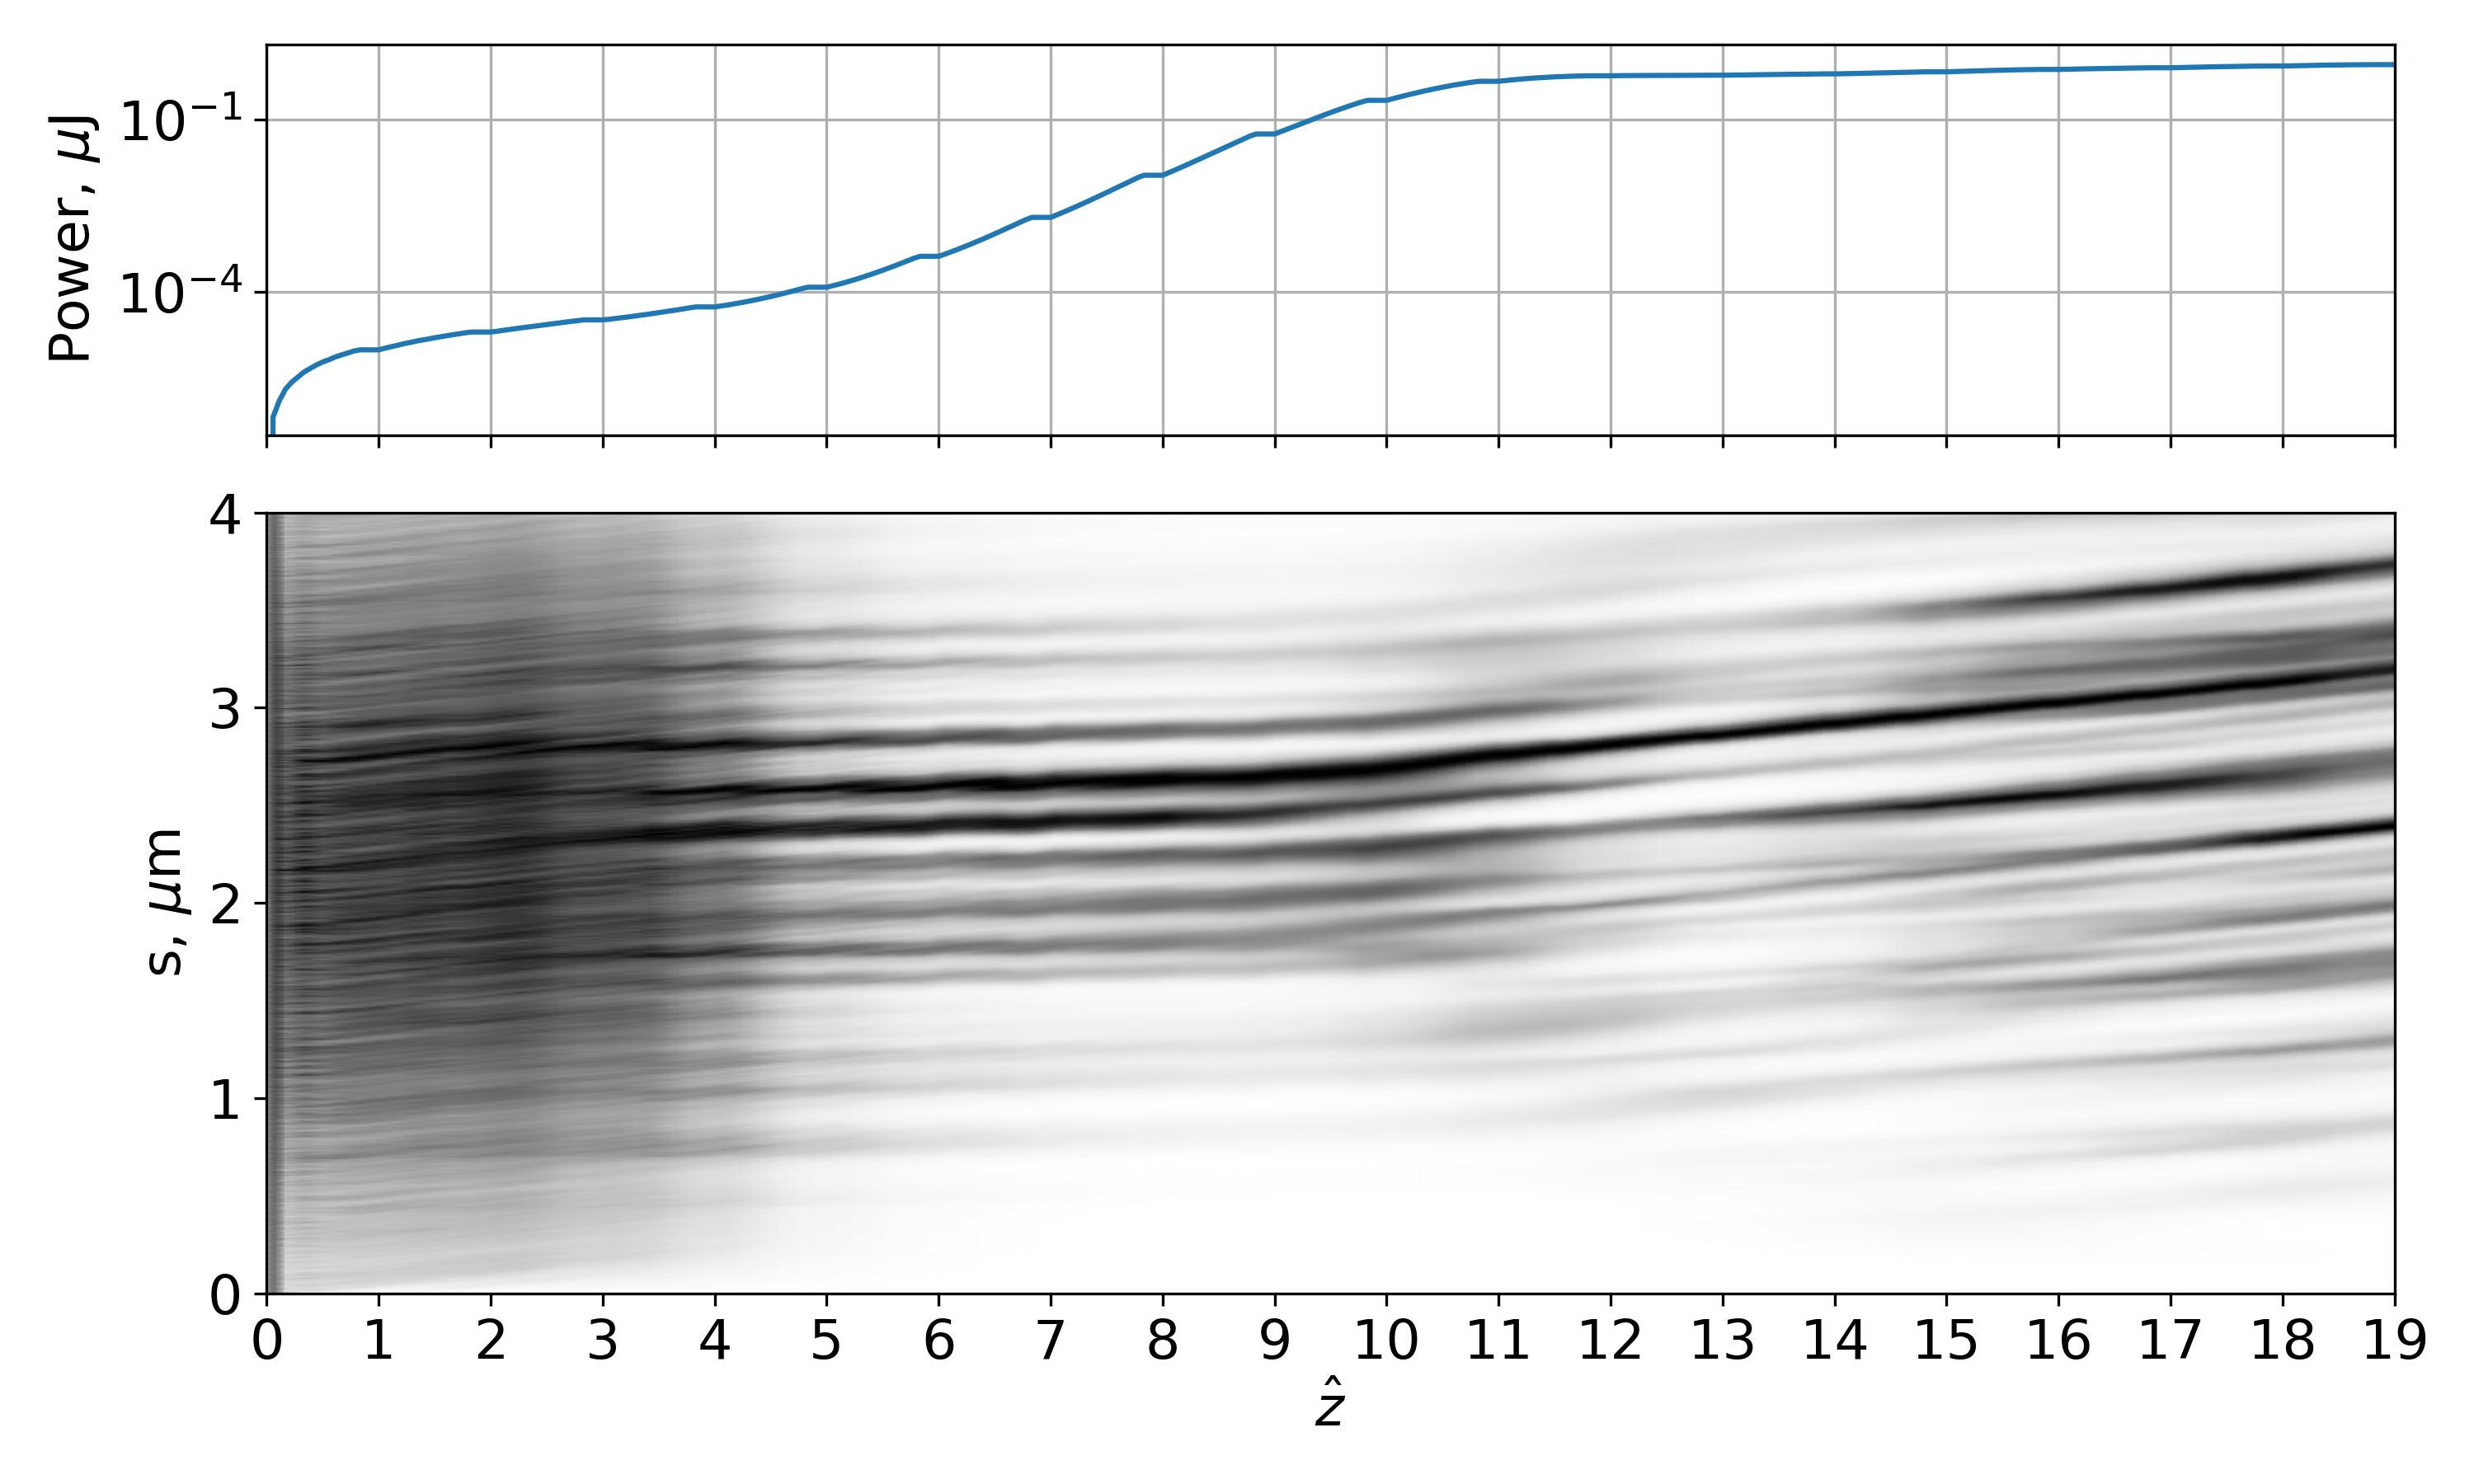
\includegraphics[width=0.95\linewidth]{content/images/4_FEL_Theory/evo_spikes.png}
\captionsetup{justification=centering}
    \caption{}
    \label{fig:pole}
\end{figure*}

\begin{figure*}[h!]
	\centering
    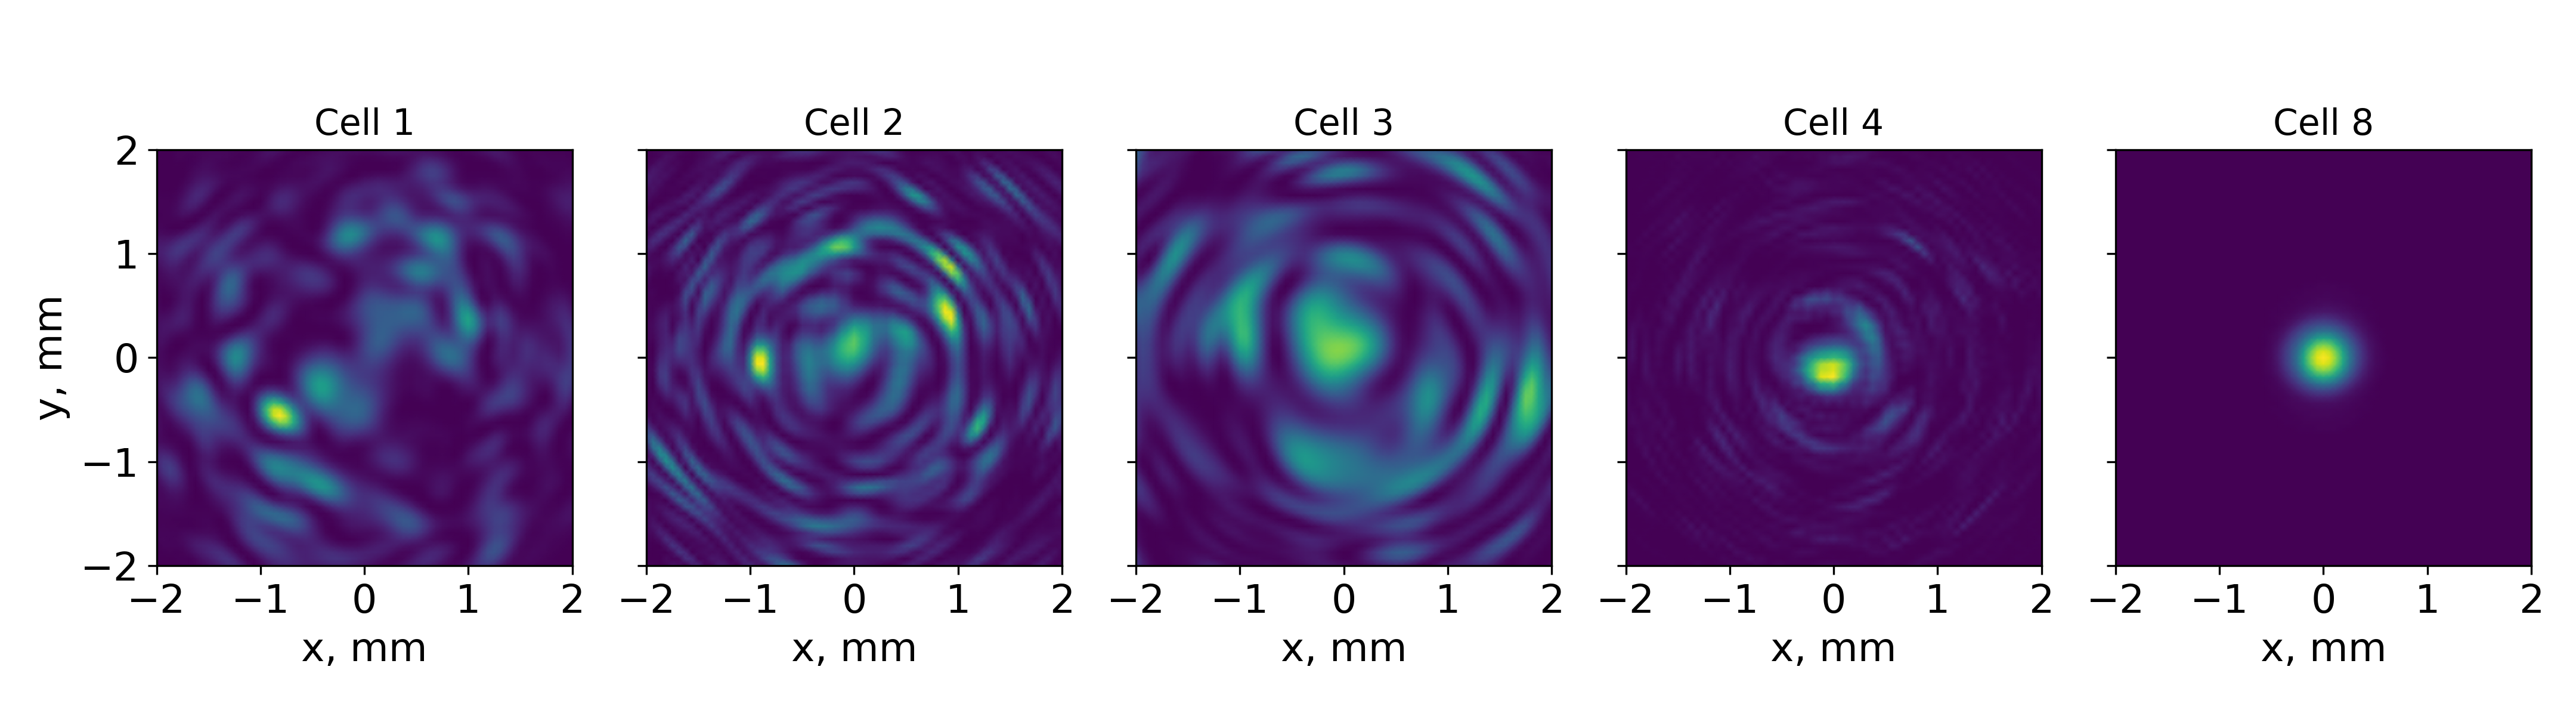
\includegraphics[width=1.1\linewidth]{content/images/4_FEL_Theory/transverse_modes.png}
    \captionsetup{justification=centering}
    \caption{}
    \label{fig:pole}
\end{figure*}
\rr{write about Gaussian statistics}\\
\rr{write about chirps}

\subsection{Heuristic approach: quasi- homogeneous/stationary source with chirps}
    Here I start with definition of the Wigner function distribution 
    \begin{align}
        \mathcal{W}(\bar{t}, \bar{\omega}) = \int \limits_{-\infty}^{\infty} \Tilde{\Gamma}(\bar{\omega}, \Delta \omega) e^{-i\Delta \omega \bar{t}}d(\Delta \omega)
    \end{align}
    One may notice that for a source that can be represented $\Tilde{\Gamma}(\omega, \Delta \omega) = f_{\omega}(\Delta \omega)\bar{I}(\bar{\omega})$ the integral factorises and as a result $\mathcal{W}(t, \omega)$ can be written as the following:
    \begin{align}
        \mathcal{W}(\bar{t}, \bar{\omega}) = \bar{I}(\bar{\omega}) \int \limits_{-\infty}^{\infty} f_{\omega}(\Delta \omega) e^{-i\Delta \omega \bar{t}}d(\Delta \omega) = \bar{I}(\bar{\omega}) I(\bar{t})
    \end{align}
    This representation hints that \rr{previous SERVAL formula} is actually represent factorized representation (by in spatial domain) and this equation can be modernised for use of the Wigner function:
    \begin{align}
    	\phi(\bar{\omega}) = \int \limits_{-\infty}^{\infty} \sqrt{\mathcal{W}(\bar{\omega}, \bar{t})} \mathcal{N}(\bar{t}) e^{i \bar{\omega} \bar{t}} d\bar{t}.
    	\label{Eq:Field_Wigner}
    \end{align}
    \subsection{SERVAL2 paper}
    \includepdf[pages=-]{content/papers/SERVAL2.pdf}


\section{Radiation at harmonics paper}
\includepdf[pages=-]{content/papers/attoharm.pdf}

\chapter{Electron beam size measurements with
direct spikes measurements of synchrotron radiation at free-electron laser facilities}
\label{chapter:CUCTUS}

    In this chapter, I present the results of measuring the electron beam size at the European XFEL free-electron laser facility using the intensity non-interferometry technique with synchrotron radiation. For this technique, it is sufficient to use a synchrotron radiation imager paired with an undulator commissioning crystal monochromator at Bragg's angle. By measuring the transverse intensity correlation, I retrieved the electron beam size at the undulator cell where this radiation was emitted. I tested this technique at the hard X-ray SASE1 and SASE2 beamlines of the European XFEL.

\section{Introduction}

    The method is based on a Hanbury Brown and Twiss-type experimental setup~\cite{cite}, where the subtended size of the radiation is determined by auto-correlating its intensity in the far zone using the results of the van Cittert–Zernike theorem. Following this pioneering experiment by Hanbury Brown and Twiss, this technique spread to various areas of physics research such as~\cite{cite it from Singer's work}. \textit{(To be continued...)}
    
    The Hanbury Brown and Twiss-type experiment not only measured the angular size of Sirius but also implicitly proved that solar radiation is stochastic. Although it has not been conclusively shown until modern times that thermal electromagnetic fields are fluctuating fields~\cite{cite}, both in the time and spatial domains (or their reciprocal pairs), the authors of~\cite{cite} directly demonstrated transverse solar radiation "speckles." Another example of stochastic radiation is SASE FEL radiation. In the FEL community, field fluctuations are referred to as spikes, despite the term speckles being commonly accepted. The motivation for this terminology is that speckles refer to the random interference of coherent light on a statistical object upon propagation, whereas spikes refer to the inherent structure of the radiation source. It was first shown theoretically~\cite{cite} and then experimentally that SASE spectra (a single shot event) consist of spikes, which clearly indicate the randomness of the process. This property is inherited from the shot noise in the electron beam. As SASE essentially starts from synchrotron radiation, one would expect to observe spikes in synchrotron radiation structure too, both in the time and spatial domains. The typical size of the spikes is the corresponding coherence length. So, the goal of this study is to reveal transverse spikes of SR directly and prove that SR is also a fluctuating field in the transverse domain. I depict SASE radiation at the early stages of amplification in Fig.…
    
    \textit{(Insert figure of 3D SASE at start)}
    
    Although it is possible to measure the transverse correlation function of the radiation with interferometric techniques, e.g., double slit, there have not been direct measurements of the single-shot events of the SR radiation that would reveal its fluctuating field. In a remarkable experiment that is presented in~\cite{cite} the authors built a high-resolution monochromator with unprecedented resolving power to resolve SR longitudinal spikes (modes) at the \textit{Spring-8} facility and measure pulse duration. At the time, there was no appropriate imager to detect the transverse distribution of the single-shot events. This experiment was later complemented with measurements of the transverse coherence length~\cite{cite} of synchrotron radiation using a setup similar to the Hanbury Brown and Twiss-type experiment. In this way, the authors retrieved the electron beam size.
    
    In this paper, I present the first measurements of the SR transversely spiky structure. 
    At the moment the present imager at European XFEL did not allows visually determine the spiky content of the recorded events, so I performed the cross-correlation analysis to recover the typical size of the spikes at the images. Then by determining the typical size of these spikes, in other words, the transverse coherence length, I retrieve the electron beam size, similar to what was done in~\cite{rr}. 
    
    I also discuss the practical use of the method for optimizing the FODO lattice and subsequently SASE performance. The recent advancements in creating femtosecond-order pulses~\cite{cite}, or even shorter, at FELs necessitate electron beam diagnostic tools to accurately manipulate the electron beam phase space. This becomes especially important when dealing with transversely tilted electron beams exhibiting a substantial energy chirp. \textit{(Write about HXRSS optimization)}. Under such circumstances, a comprehensive understanding of the transverse electron beam characteristics along the entire FEL undulator line becomes essential for optimizing SASE performance.
    
    This chapter is organized as follows: first, I will estimate the parameter space in terms of the expected contrast of the images I record, as well as the possibility of spatially resolving the sought correlation function. Then, I present the method I utilized to perform correlation analysis. Subsequently, I show the simulation results that replicated the expected radiation behavior. In the real experiment, the signal is so low that the signal-to-noise ratio in most cases falls below unity. Therefore, I upgraded the correlation analysis. This upgrade relies on the fact that the radiation is quasi-homogeneous, allowing for averaging over auto-correlation function anti-diagonals to effectively increase statistics. Finally, I present the experimental results, where I observed a significant level of correlation. I estimated its width and retrieved the electron beam size. I conclude the chapter with a discussion on the possible implementation of the method in BKR of the European XFEL and issues to be addressed in the future.
    
\section{Underlining theory}

\subsection{Qualitative estimations}
    As was mentioned in the introduction synchrotorn radiation possesses spike structure in both domain longitudinal and transverse. As one would detect this radiation  monochromotised and in the far zone it make sense to setup ones thinking in frequency-inverse space domains. In this representation of the radiation each longitudinal spike in the frequency domain will contain its unique transverse spiky distribution in inverse space domain. In essence, the typical width of these spikes is the spectral correlation function, which in other words means that transverse spikes are statistically independent of each other. So, I what one would observe a a convectional synchrotron radiation source based on a storage ring is a smoothed transverse radiation distribution upon monochromatisation. This happens do to relately long of order of dozens pico second electron beam duration that defines that radiation pulse duration as well. As longitudinal coherence length is much less than this pulse duration one would expect to observe immense number of the spikes in longitudinal domain even upon monochromatization with a conventional monochromator. This is the reason why the authors of~\cite{} built such a unique monochromator to resolve spikes in frequency domain, which was essential for their measurements.

    \begin{figure*}[h!]
    	\centering
        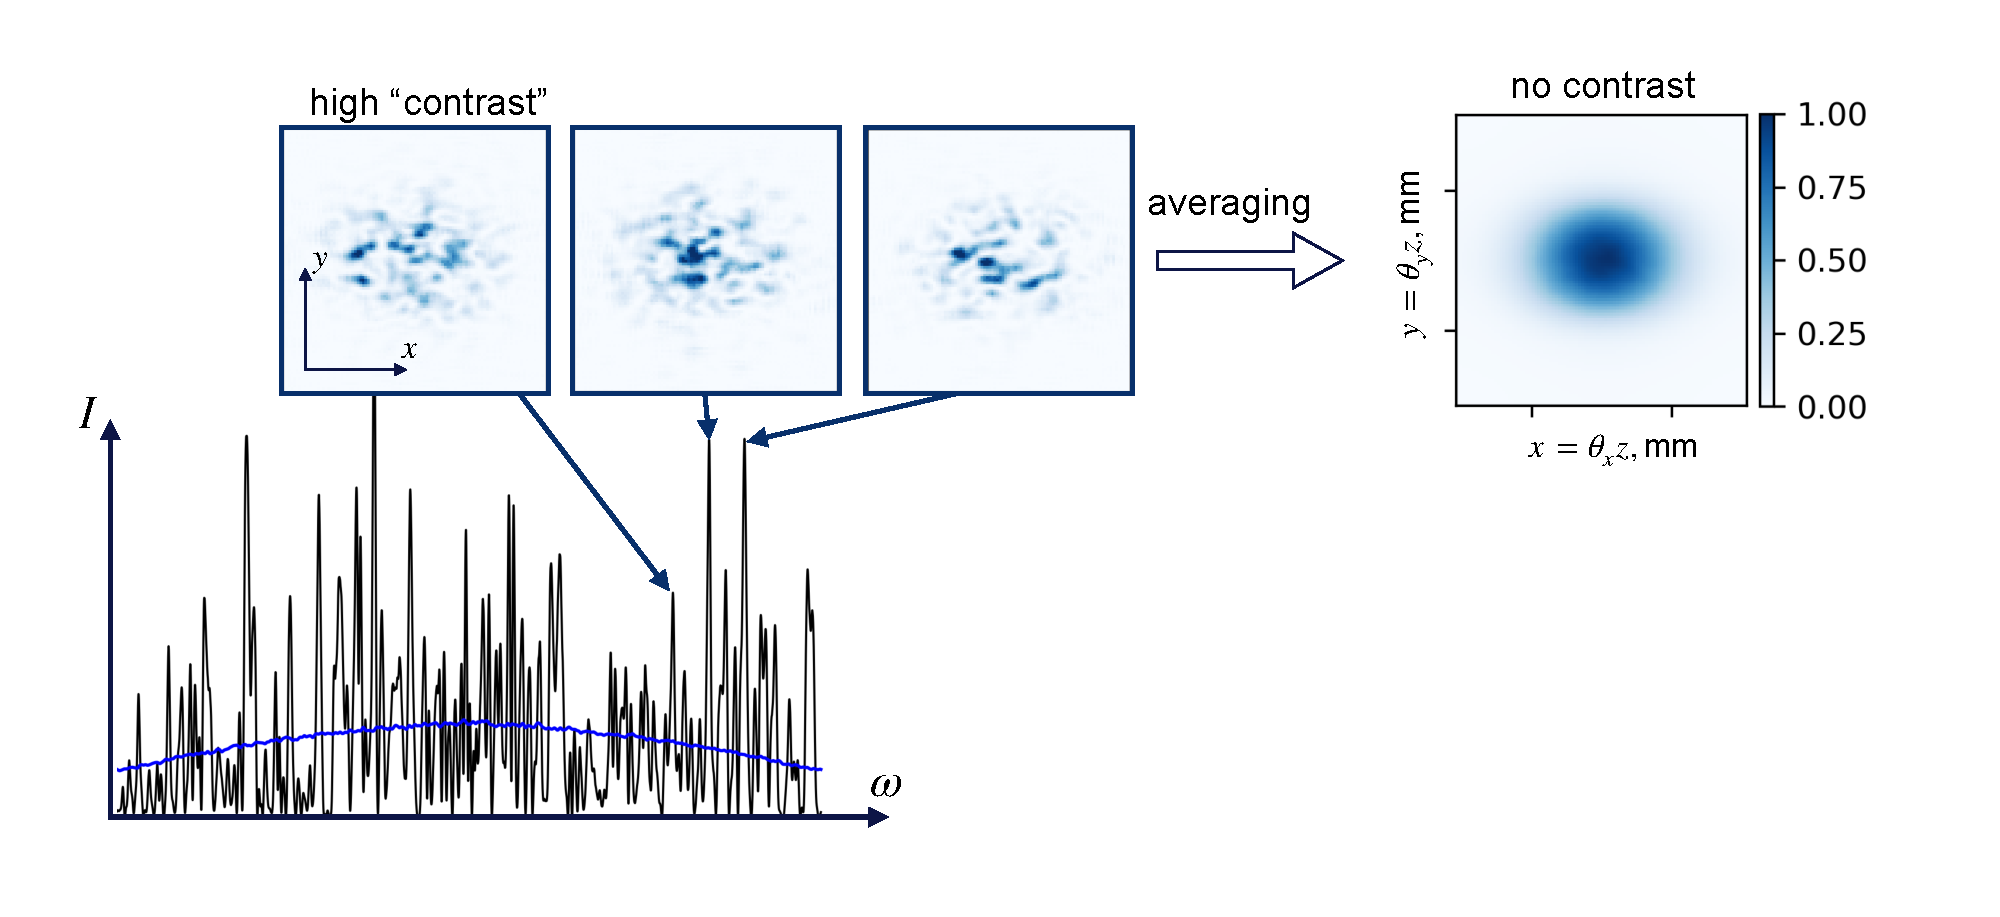
\includegraphics[width=0.99\linewidth]{content/images/ebeam_size_with_SR/SR_spikes_many.pdf}
        \captionsetup{justification=centering}
        \caption{}
        \label{Fig:SR_spikes_many}
    \end{figure*}

    The situation is radically different parametrically-wise at linear accelerator facilities such as European XFEL. The duration of the electron beam are at the dozen of femtosecond level. This why if one use just a single undulator cell to generate usual synchrotron radiation there will be much fewer longitudinal spike upon monochromatisation with a conventional crystal monochromator with Si~(111) reflection, as shown in Fig.~\ref{Fig:SR_spikes_few}. Then at an imager one would observe effective averaging of the spikes distribution that are contained in the longitudinal spikes. As a result averaging over several dozens of the longitudinal spikes will result in a low contrast transverse distribution, that will still will contain the imprint of the spikes, what I show in Fig.~\ref{Fig:SR_spikes_few} in the red-framed subplot. This result is only possible with an ideal imager, in real case scenario the resulting image may be heavily affected by noise.

    \begin{figure*}[h!]
    	\centering
        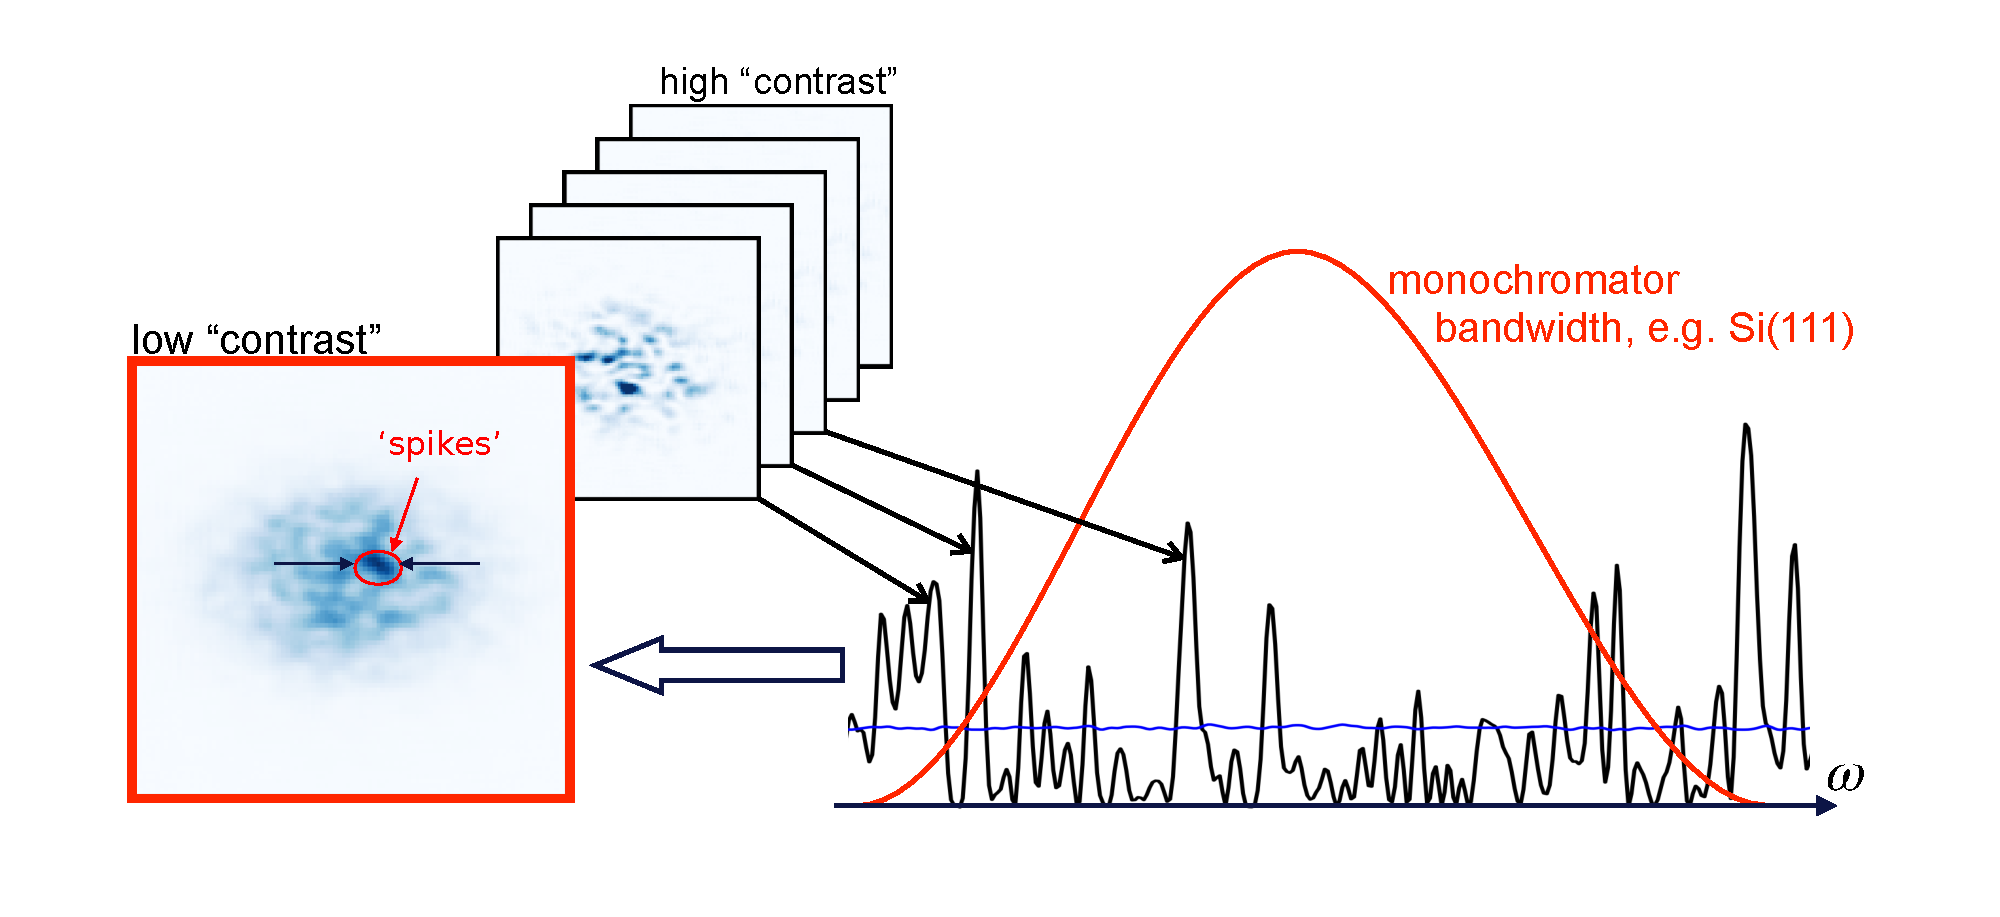
\includegraphics[width=0.99\linewidth]{content/images/ebeam_size_with_SR/SR_spikes_few.pdf}
        \captionsetup{justification=centering}
        \caption{}
        \label{Fig:SR_spikes_few}
    \end{figure*}

    So, is one collect enough statistic of these averaged images and then calculate the typical size of these spikes then on would be able tho retrieve the electron beam size. Before proceeding to this analysis part I will provide more qualitative estimation on the expected contrast of the image and required spatial resolution of the imager.
    
\subsection{Quantitative estimations}
    At first I estimate number of longitudinal spike that on cut out with a silicon based monochromator under Brag's angle using (111) reflection. Knowing typical spike width and the resolution of Si~(111) I plot the dependence of the amount of spike extracted with the monochromator versus pulse duration and undulator radiation resonance frequency in Fig.~\ref{Fig:M_L} calculated with Eq.~\ref{Eq:M_L}:
    \begin{align}
        M_L = \cfrac{2\sqrt{2 \textup{ln}(2)} \sigma_{ebeam} \Delta E}{h}.
        \label{Eq:M_L}
    \end{align}
    
    \begin{figure*}[h]
    	\centering
        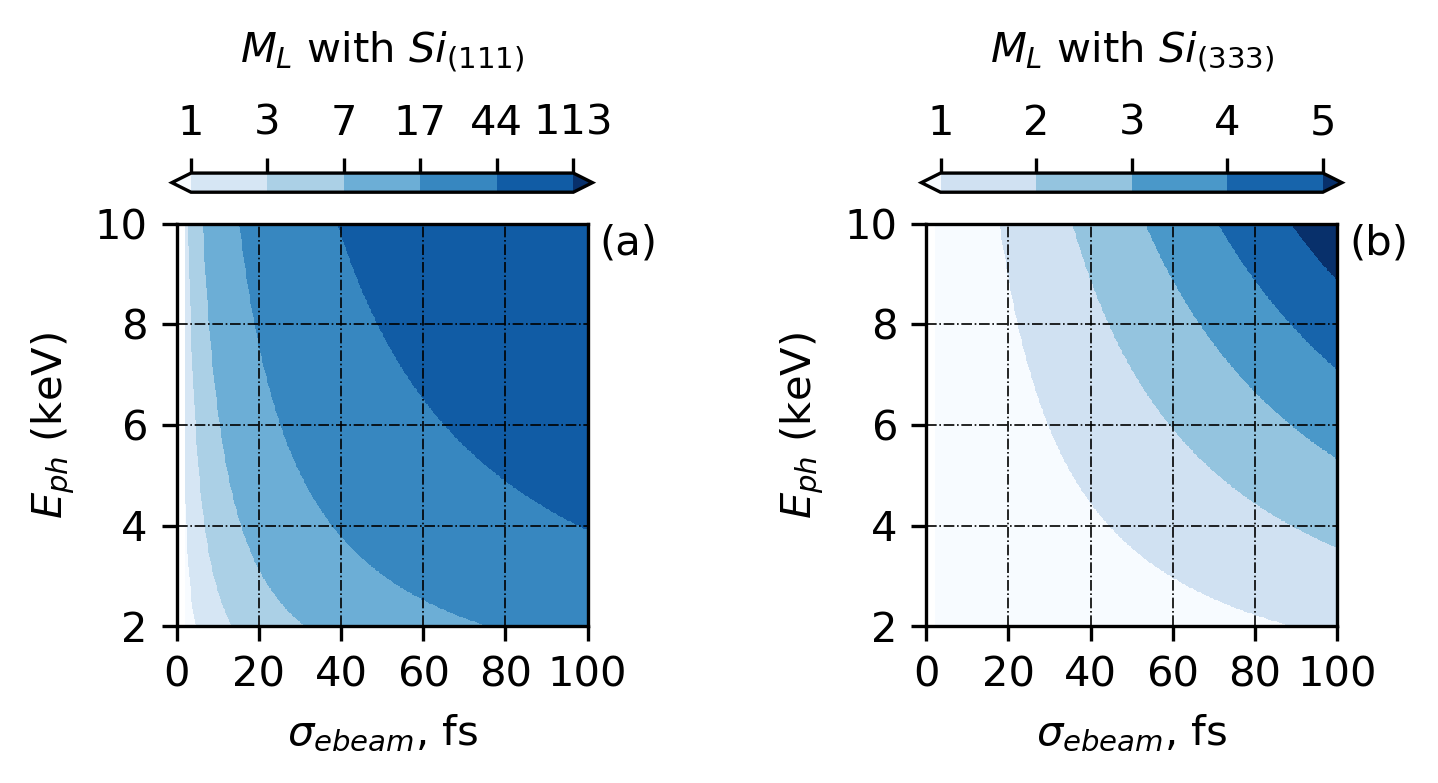
\includegraphics[width=0.63\linewidth]{content/images/ebeam_size_with_SR/M_L.png}
        \captionsetup{justification=centering}
        \caption{}
        \label{Fig:M_L}
    \end{figure*}

    In term of the spacial resolution required to resolve the correlation function I plot the distributions in Figs.~\ref{Fig:cell_2},~\ref{Fig:cell_18}, and~\ref{Fig:cell_37} where I depict the resulting correlation function versus electron beam transverse size and used undulator radiation  resonance frequency.
    \begin{figure*}[h!]
        \centering
        \begin{subfigure}[b]{0.32\textwidth}
            \centering
            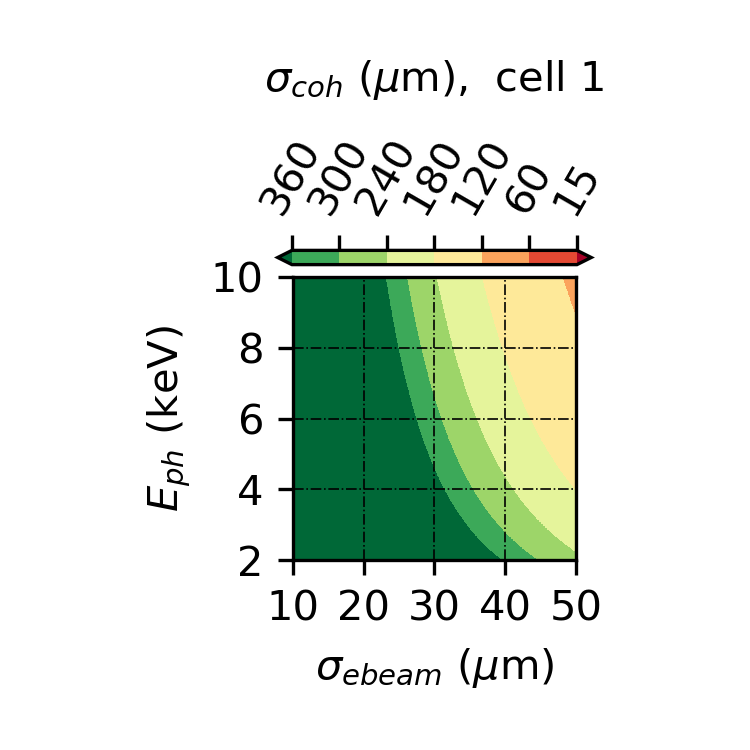
\includegraphics[trim={0.4cm 0 0.4cm 0}, clip, width=\textwidth]{content/images/ebeam_size_with_SR/cell 1.png}
            \caption{Caption for the first figure}
            \label{Fig:cell_2}
        \end{subfigure}
        \hfill % Use \hfill to add horizontal space between figures
        \begin{subfigure}[b]{0.32\textwidth}
            \centering
            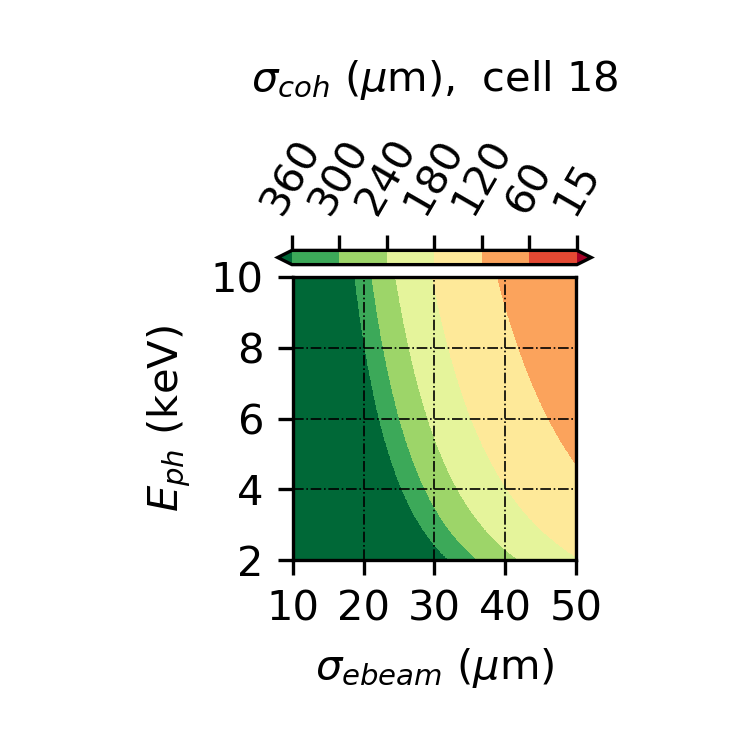
\includegraphics[trim={0.4cm 0 0.4cm 0}, clip, width=\textwidth]{content/images/ebeam_size_with_SR/cell 18.png}
            \caption{Caption for the second figure}
            \label{Fig:cell_18}
        \end{subfigure}
        \hfill % Use \hfill to add horizontal space between figures
        \begin{subfigure}[b]{0.32\textwidth}
            \centering
            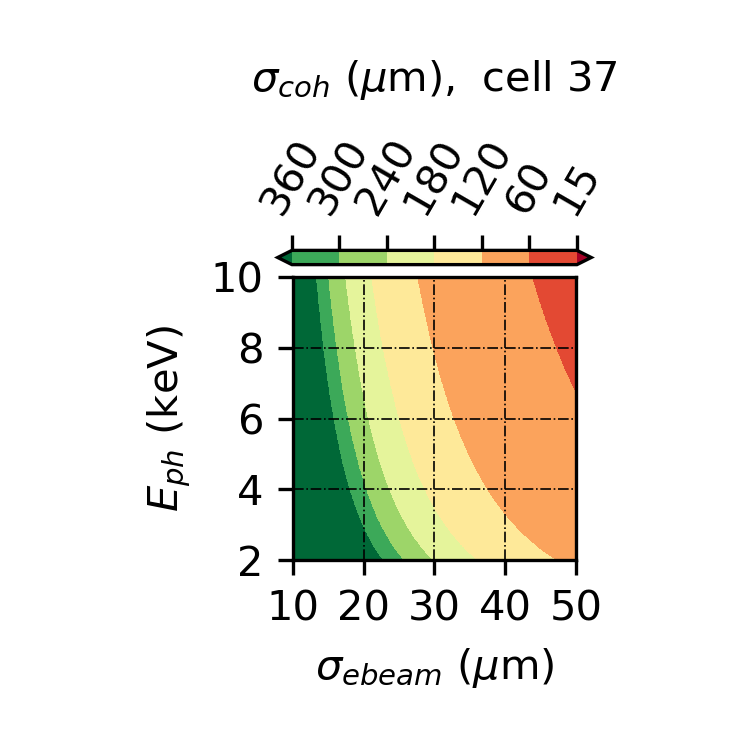
\includegraphics[trim={0.4cm 0 0.4cm 0}, clip, width=\textwidth]{content/images/ebeam_size_with_SR/cell 37.png}
            \caption{Caption for the third figure}
            \label{Fig:cell_37}
        \end{subfigure}
        \caption{General caption for all figures.} % Optional: General caption for all subfigures
    \end{figure*}
    It is clear from these estimations that it is more then possible to see spikes in transverse dimension after monochromatization. In the next section I will show the simulation of the real experiment that was conducted at European XFEL. I also in detail describe the raw data processing procedures to extract information about the correlation function.
    
\section{Simulation}
    I replicated the experimental results in the simulation using SERVAL algorithm presented before in the thesis. In Fig.~\ref{Fig:int_corr_1event} I present 
    \begin{figure}[h!]
    	\centering
        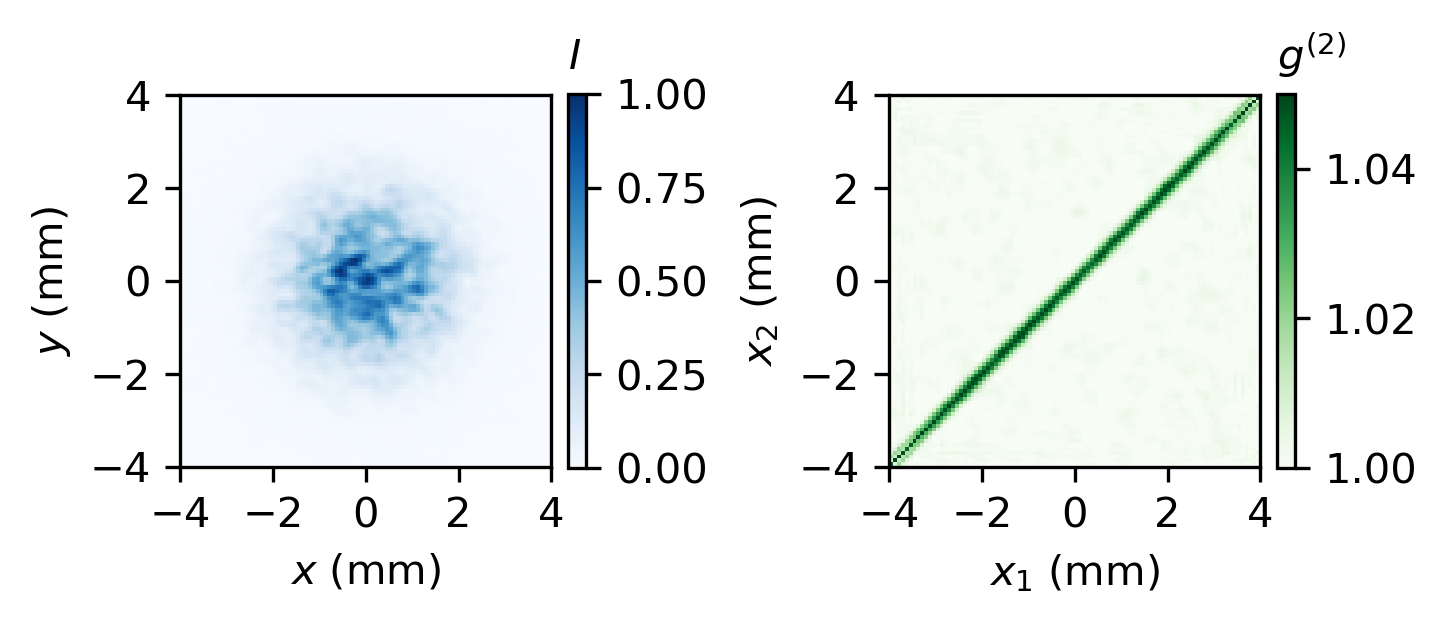
\includegraphics[width=0.66\linewidth]{content/images/ebeam_size_with_SR/int_corr_1event.png}
        \captionsetup{justification=centering}
        \caption{}
        \label{Fig:int_corr_1event}
    \end{figure}

    \begin{figure}[h!]
    	\centering
        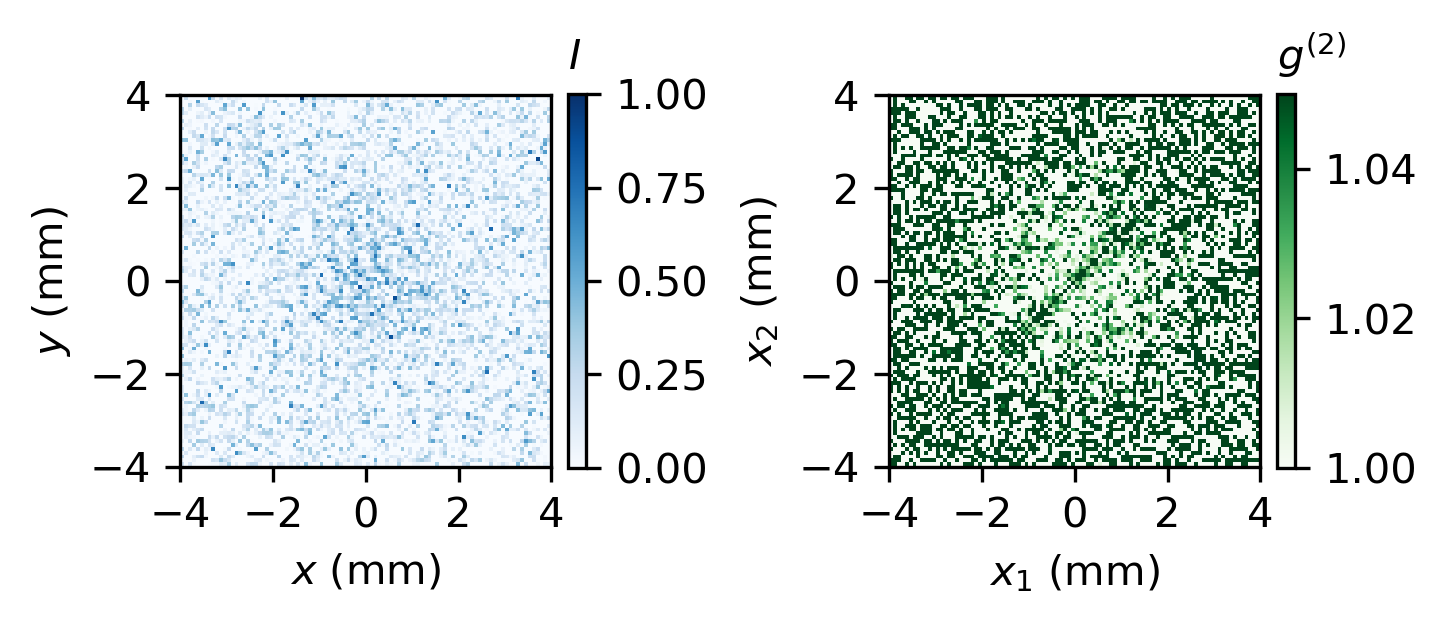
\includegraphics[width=0.66\linewidth]{content/images/ebeam_size_with_SR/int_corr_1event_noise.png}
        \captionsetup{justification=centering}
        \caption{}
        \label{Fig:int_corr_1event_noise}
    \end{figure}

    \begin{figure}[h!]
    	\centering
        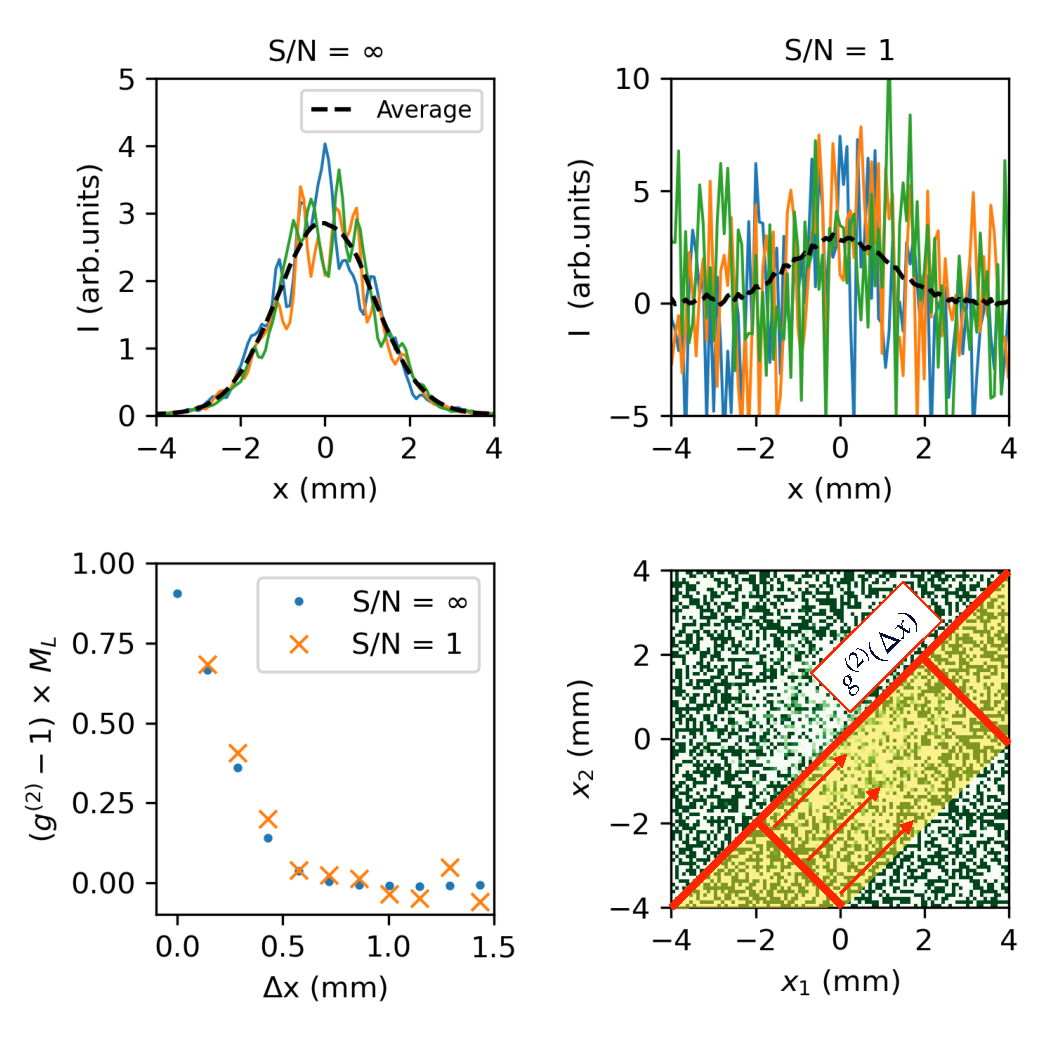
\includegraphics[width=0.66 \linewidth]{content/images/ebeam_size_with_SR/triangle_mod_full.pdf}
        \captionsetup{justification=centering}
        \caption{}
        \label{Fig:triangle}
    \end{figure}
\section{Experimental results}

    The experiment for measured the transverse coherence of SR at European XFEL was done at SASE1 and SASE2 beamlines of the facility. This beamlimes are equipped with K-mono -- a undulator commissioning monochromator --, and a SR imager. 
    
    
\section{Outlook and discussion}

\section{Conclusion}
\chapter{Code for calculating synchrotron radiation in a waveguide}
\label{chapter:Synchrotron_radiation_in_a_wave_guide}

\rr{correct the intro where it's not actual with what was presented}
\rr{all citations will be included later (I have all them in mind, but inserting them is a bit tedious and distracting from writing)}
\rr{probably add the name of the code SRinWG of SRinWaveGuide}
    
    Generation of synchrotron radiation is typically considered in free space, where the problem adheres to a natural boundary condition: the field diminishes to zero at infinity. This assumption serves as a practical approximation since, even though at the real facilities radiation is generated and propagates within vacuum pipes and faces another components like mirrors, apertures, flanges, detectors etc, their influence on radiation in a wide range of wavelengths (from visible light up hard X-ray and higher) is often negligible to an undetectable level. However, when dealing, for instance, with THz radiation it becomes necessary to consider the effects of these metallic components on the radiation, especially the vacuum pipes. In this chapter, I introduce a numerical code that is designed to calculate synchrotron radiation in the presence of boundary conditions of perfectly conducting metallic walls… \rr{say that the walls are considered to be perfectly conducting and what would be the result with normal medium}
    
    Theoretical background for this problem was founded in~\rr{cite}, that extends and complement prior works~\rr{cite}. The goal of this work is to develop a code based on derivation made in~\rr{cite} capable of accurately calculating synchrotron radiation accounting for the waveguide effects, e.g. imposed by the metallic components of the beamlines. This is essential for the precise numerical simulation of the performance of insertion devices at THz beamlines. Such a tool is crucial for designing THz radiation propagation lines at facilities, including those planned or under construction at SLAC~\rr{cite} and the European XFEL~\rr{cite}, as well as those had been already in operational e.g. FLASH, \rr{is there more}. The method I employed to program a code utilizes the Green's function approach to solve the field equation. This approach offers considerable flexibility; once the Green's function for a given system is determined—which can be usually analytically derived for simple, yet practical geometries—one only needs to take an integral over the right-hand side of the wave equation. The right-hand contain an electron trajectory and velocity that can easily can be found analytically or solving this numerically with tools like those~\rr{cite}
    
    Within this chapter, I deduce the boundary conditions for a waveguide with an arbitrary cross-section, present the general form of the integral that is to be taken, and provide the expression for the Green's function for an axially symmetrical metallic waveguide based on~\rr{cite}. A significant part of this chapter is dedicated to cross-validating the developed code. The verification process begins with a straightforward scenario of synchrotron radiation in free space using corresponding Green's function of the Helmholtz equation. This step is done to cross-check the integration process itself. The results of the developed code I cross-check with Synchrotron Radiation Workshop (SRW)~\rr{cite}. Only then I cross-validate the results obtained with the Green's function of a circular waveguide. I test the results in the limit of free space: I take the waveguide Green's function, increase the tube's radius ($R$), and compare these results with those obtained using the free space Green's function. Finally, in a real scenario where there is a strong influence of the walls for a ten-period undulator device, I cross-check the results of the code with analytical expressions.
    
    The developed code has been uploaded to a GitHub repository~\rr{cite}, with plans for further development to meet the demands of accurate THz radiation beamline simulations. The development and cross-checks of the code have revealed several challenges that necessitate further studies. For instance, the Green's function of the bounded system is an infinite sum of transverse modes, and identifying which of these modes effectively contribute to the integral beforehand is crucial: some modes lead to the appearance of highly oscillatory integrals, which result in aliasing issues, while their contributions are negligible. Additionally, enhancements are needed in the code's numerical efficiency, along with addressing other programming-related issues in potential future work.
    
\section{Boundary conditions}
    
    In Chapter~\ref{chapter:Synchrotron radiation}, I considered the solution of the wave equation for a single electron moving on an arbitrary trajectory in free space within the paraxial approximation. This treatment will now be extended to the case of a single electron moving in a magnetic field in the presence of \rr{perfectly conducting} metallic boundaries. Before deriving formulas and accounting for the boundary conditions, one must assume that the waveguide is overmoded for the given wavelength, e.g., $\lambdabar \ll R$, following~\rr{cite}, to ensure that the slowly varying envelope approximation can be applied. Additionally, one needs to confirm the applicability of the paraxial approximation in the presence of a waveguide, which generally holds when $k_{\perp}^2 c^2 / \omega^2 \ll 1$, where $k_{\perp}$ is the transverse wave number. To extend this to the case with the waveguide, this condition should also hold for each mode in the waveguide.
    
    For the metallic walls boundary conditions means that the electric field must be perpendicular to the surface ($S$).
        \begin{align}
            \left(n_x \widetilde{E}_y - n_y \widetilde{E}_x\right)_{\big|_S}=
            \left(\vec{n} \times \vec{\widetilde{E}}_\bot\right)_{\big|_S} = 0
        \end{align}
    and 
        \begin{align}
            \left(\widetilde{E}_{z}\right)_{\big|_S}= 0.
        \end{align}
    One of the Maxwell's equation for the curl of the magnetic field can be written as the following:
        \begin{align}
            \left[\left(\vec{\nabla} \times \vec{\widetilde{H}} \right)_{z}\right]_{\big|_{S}}= 0. 
        \end{align}
    And in the paraxial approximation we make use of the relation for the magnetic field and electric: $\widetilde{E}_x \simeq \widetilde{H}_y$ and $\widetilde{E}_y \simeq -\widetilde{H}_x$. Having both of the conditions: on the amplitude of the field and on its derivatives I write:
        \begin{align}
            \left(\frac{\partial \widetilde{E}_x}{\partial x} + \frac{\partial
            \widetilde{E}_y}{\partial y}\right)_{\big|_{S}} =
            \left(\vec{\nabla}_\bot \cdot
            \vec{\widetilde{E}}_\bot\right)_{\big|_S} = 0
        \end{align}
    So, writing together the wave equation and the boundary condition I obtain the following system:
        \begin{align}
            \left\{
            \begin{array}{l}
            \mathcal{D} \left[\vec{\widetilde{E}}_\bot(z,\vec{r}_\bot)\right]
            = \vec{f}(z, \vec{r}_\bot)
            \\
            \left(\vec{n} \times \vec{\widetilde{E}}_\bot\right)_{\big|_S} = 0
            \\
            \left(\vec{\nabla}_\bot \cdot
            \vec{\widetilde{E}}_\bot\right)_{\big|_S} = 0~,
            \end{array}\right.
            \label{Eq:boundary_conditions}
        \end{align}

    This system should be solved for the given vacuum pipe shape. One can find the solutions for a general case of an arbitrary shape and for the circular waveguide in~\rr{cite}. Once the Green's function is known the slowly carrying envelope of the electron field is written in the following form:
    \begin{align}
        \widetilde{E}^{\alpha}(\vec{r}_\bot,z) = \int_{-\infty}^{z} dz'
        \int d\vec{r'}_\bot~ G^\alpha_\beta\left(\vec{r}_\bot,
        \vec{r'}_\bot,z-z'\right) f^\beta\left(\vec{r'}_\bot,z'\right),
        \label{Eq:field_integral_tensor}
    \end{align}
    or writing it explicitly:
    \begin{align}
        &&\widetilde{E}^\alpha = \frac{4\pi e}{c} \int_{-\infty}^{z} dz'
        \left\{ \frac{i\omega}{c^2} \fcolorbox{black}{blue!30}{$\stackrel{\text{velocity term}}{v_\bot^\beta(z')
        G^\alpha_\beta\left(\vec{r}_\bot,\vec{r'}_\bot(z'), z-z'
        \right)}$}+\fcolorbox{black}{orange!30}{$\stackrel{\text{gradient term}}{\partial'_\beta
        G^\alpha_\beta\left(\vec{r}_\bot,\vec{r'}_\bot(z'), z-z'\right)}$}
        \right\}\cr &&\times \exp\left[\frac{i\omega}{2c} \int_0^{z'}
        \frac{d\bar{z}}{\gamma^2_z(\bar{z})} \right].
        \label{Eq:field_integral_tensor_full}
    \end{align}
    \rr{what is the integration limits for the second integral?}
    The integral contains the Green's function $G^\alpha_\beta$ that is actually not a scalar value but a tensor.

    This integral should be calculated with a given Green's function. As one can see, it is possible to use any Green's function; in this sense, the problem is divided into two steps. First, one needs to derive or calculate a Green's function for a given system, which is basically the solution to the eigenvalue problem for the operator $\mathcal{D}$, including the boundary condition from the system in Eq.~\ref{Eq:boundary_conditions}. Then, take the integral in Eq.~\ref{Eq:field_integral_tensor} that is composed from the right-hand side of the wave equation in Eq.~\ref{Eq:boundary_conditions}. I explicitly take the integral. The uniqueness of this approach is that any Green's function, once known, can be substituted as an input in the code, and the field distribution can be calculated.


\section{Numerical algorithm}
    In this section, I provide detail on the calculation algorithm for taking integral under Eq.~\ref{Eq:field_integral_tensor_full}. For evaluating the field $\widetilde{E}^\alpha$ one need to calculate the integrant expression, which include: taking the integral $\int_0^{z'}
    d\bar{z}/\gamma^2_z(\bar{z})$, calculating the velocity term, and estimating the gradient term. 
    
    Integration for both integrals is performed trivially and can be made with variety of the integration rules: rectangle rule, trapezoidal rule, and more advanced Gauss–Legendre quadrature formula with three points, which provide the accuracy of $\mathcal{O}(h^{1})$, $\mathcal{O}(h^{2})$, and $\mathcal{O}(h^{5})$ with respect to grid spacing, where $\mathcal{O}$ is Big O notation or Bachmann–Landau notation. Simpson's rule with accuracy order of $\mathcal{O}(h^{4})$ shall to be implemented, although I used trapezoidal rule in the following cross-checks being more accurate then trivial rectangle rule and faster then using Gauss–Legendre quadrature formula. For practical applications in numerical simulation this level of accuracy is enough.

  

    As the end goal is to write a code that can accept an arbitrary Green's function taking the derivative should be done numerically following the definition:
        \begin{align}
           f'(x) = \lim_{h \to 0} \frac{f(x + h) - f(x)}{h}, 
           \label{Eq:numerical_derivative}
        \end{align}
    where $x$ is the transverse coordinate variable of a general function $f$ and $h$ is the step along $x$. Taking the derivative numerically requires careful choice of the $h$. For this, I used an adaptive step size formula for the increment $h = \sqrt{\epsilon} x$ or $h = \sqrt{\epsilon}$ if $x = 0$, where $\epsilon$ is machine precision, to avoid rounding errors in case of small $h$ and the errors of differentiation formula itself on the the other side. This insures adequate accuracy of this formula. Interesting, the accuracy of the formula is limited by the estimation of $-f^{(3)}(c) h^2 / 6$, where $c$ is a point in between $x$ and $x + h$. The first order term in canceled naturally due to subtraction operations in Eq.~\ref{Eq:numerical_derivative}. 

    The integration and taking derivative methods can be further improved and also tested, i.e. result of the of different integration rules should be compared, there a formula for five-point method for taking the derivative etc. In the chapter I present the first result on this method and chosen accuracy integration and differentiation is enough for the purpose of cross-checks. The code will be improved at the next iteration of the development.
    
\section{Cross-checks}

    In this section, I will first cross-check the code for the free-space Green's function against the results provided by the Synchrotron Radiation Workshop (SRW) \rr{cite} to ensure the correctness of the chosen approach. It is also essential to examine the 'gradient term,' as the derivative is taken numerically, which may lead to a loss in accuracy and introduce numerical artifacts. Then, I will evaluate the code's performance for the waveguide Green's function. I will verify that the free-space limit is achieved by increasing the radius of the waveguide and subsequently compare it with the analytical expression for undulator radiation in resonance within a waveguide, as described in \rr{cite}.

\subsection{Free space Green's function}

    Typically, codes for calculating synchrotron radiation employ an expression where the free space Green's function is already substituted, and the derivative is taken analytically. Additionally, it is possible to further adjust the integral to prevent the emergence of highly oscillatory contributions, which I will discuss later in the section. This ensures a certain robustness of this approach compared to using the solution of the field equation in its general form with an arbitrary Green's function. The latter requires taking a numerical derivative, which is especially pronounced in the case of edge radiation \rr{cite}. In this instance, the code's limits of applicability should be verified.

    I will present a cross-check of the radiation field calculation results from different magnetic structures with SRW. I will examine a simple arrangement of bending magnets, a three-pole device, an undulator, and one special case, although it is not very possible from a physics perspective. I will discuss several numerical techniques to ensure the physical correctness of the resulting distributions.

\subsubsection{Bending magnet radiation}

    The bending magnet synchrotron radiation drew the attention of researchers at the dawn of synchrotron radiation studies. Despite its apparent simplicity, this source actually has a rigorously complicated structure. Specifically, it concerns the manner in which radiation forms, thereby possessing a nontrivial source structure of single electron (or filament beam) emission. \rr{cite Oleg's paper and GG work}. 
    \begin{figure}[h!]
        \centering
        \begin{subfigure}[c]{0.5\linewidth}
            \centering
            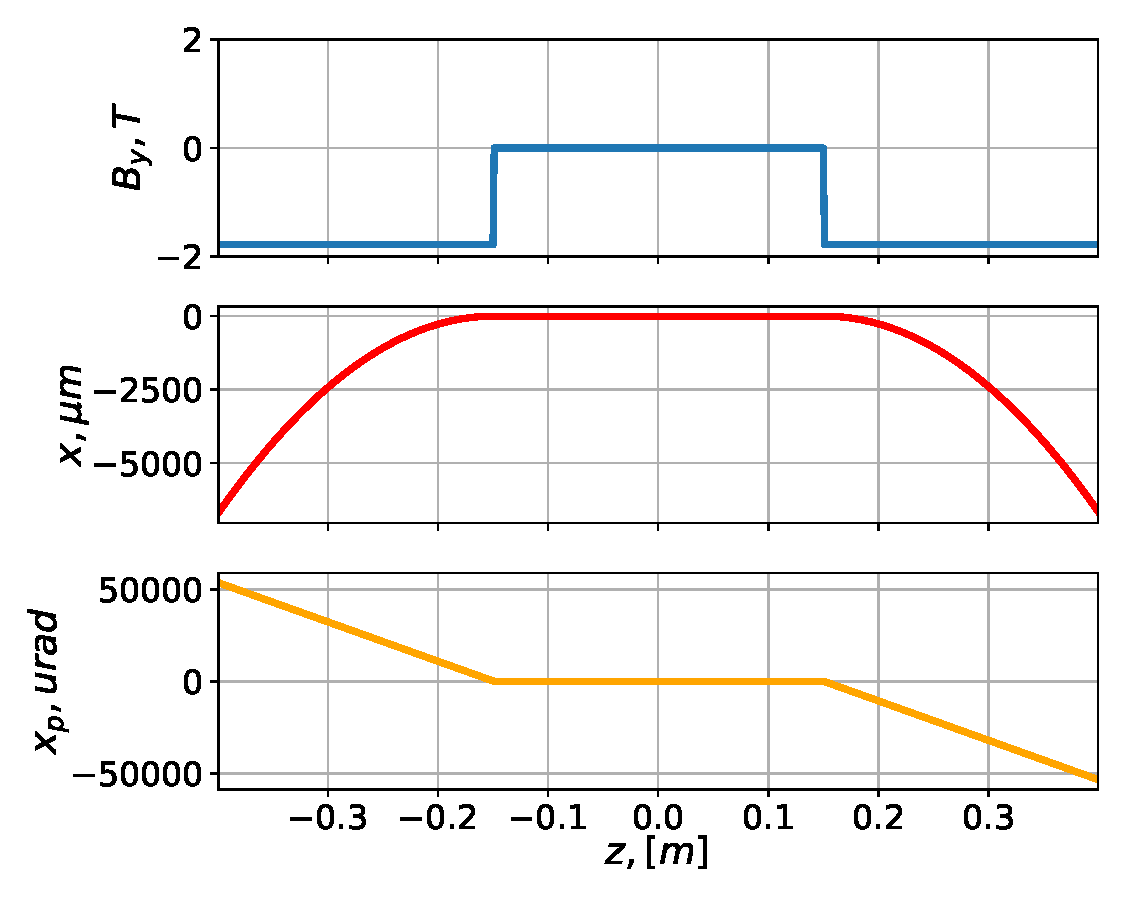
\includegraphics[width=\linewidth]{content/images/5_THz_Source/bend_traj.pdf}
            \caption{From top to bottom: $y$ component of the magnetic field, $x$ component of the trajectory and $x_p$ is the angel of the electron's direction.} % Optional individual caption for the first subfigure
            \label{Fig:bending_traj}
        \end{subfigure}%
        % Add a little space between figures if desired
        \begin{subfigure}[c]{0.5\linewidth}
            \centering
            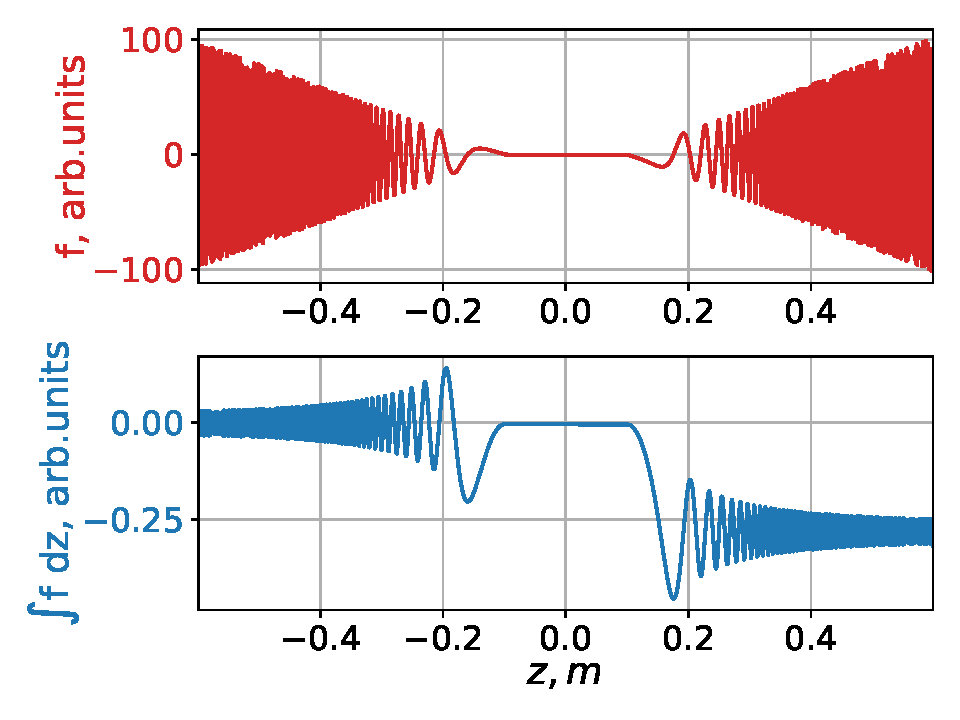
\includegraphics[width=\linewidth]{content/images/5_THz_Source/bend_integral.pdf}
            \caption{Integrant value with respect to $z$ value and corresponding integral value for the bending magnet radiation.} % Optional individual caption for the second subfigure
            \label{Fig:bending_integral}
        \end{subfigure}
        \caption{Bending magnet trajectory and integral evaluation with respect to the longitudinal coordinate.} % Optional overall caption
        \label{Fig:bending_magnet_figs}
    \end{figure}
    Also, radiation from a bending magnet can be non-trivial to calculate numerically, especially in the case of seemingly simple arrangements like the one presented in Fig.~\ref{Fig:bending_traj}. This case is chosen for the sake of cross-checking, as it encompasses all the effects that one must consider when calculating synchrotron radiation. 
    
    \begin{figure*}[h!]
    	\centering
        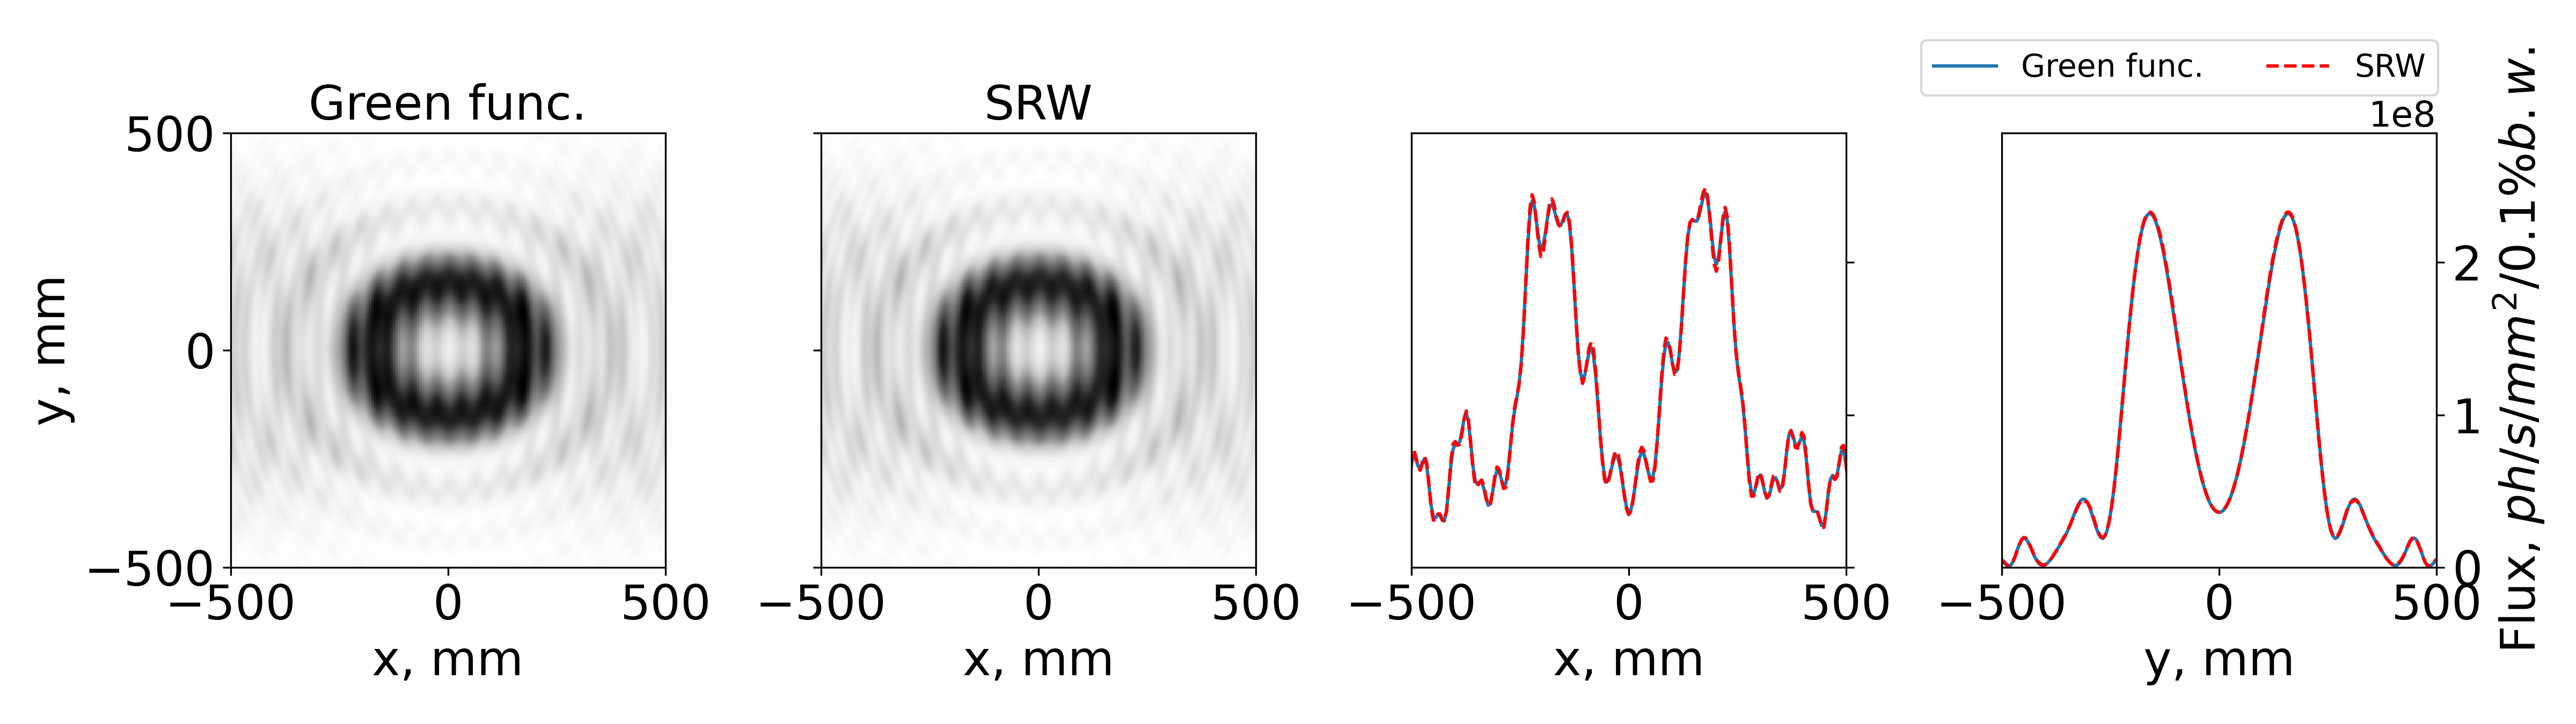
\includegraphics[width=0.95\linewidth]{content/images/5_THz_Source/bend.png}
        \captionsetup{justification=centering}
        \caption{Comparison of computational results from \rr{the developed code} and SRW for the radiation from the magnetic structure presented in Fig.~\ref{Fig:bending_magnet_figs} (arrangement of bending magnets). Total flux is presented for both polarization components.}
        \label{Fig:bend}
    \end{figure*}

    Firstly, it is observed that the integral exhibits a highly oscillatory behavior, as depicted in Fig.~\ref{Fig:bending_integral}. This characteristic can be discerned from the expression of the integral:
    \begin{align}
        \vec{\tilde{E}}_{\perp}(\vec{r}_{\perp 0}, z_0, \omega) = - \cfrac{i \omega e}{c^2}\int_{-\infty}^{\infty} dz' \frac{1}{z_0 - z'}
        \bigg[\bigg(\frac{v_x(z')}{c} - \cfrac{x_0 - x'(z')}{z_0 - z'}\bigg)\vec{e}_x + \bigg(\frac{v_y(z')}{c} - \cfrac{y_0 - y'(z')}{z_0 - z'}\bigg)\vec{e}_y\bigg] \times
        \cr \exp{\bigg[i\omega \bigg(\cfrac{(x_0 - x'(z'))^2 + (y_0 - y'(z'))^2}{2c(z_0 - z')} +  \cfrac{s(z')}{v} - \frac{z'}{c} \bigg)\bigg]}
        \label{Eq:free_space_Green_function_integral_simp}
    \end{align}
    As electrons diverge from the optical axis ($x, y = 0$ and $x_p, y_p = 0$), the phase increases, and the integral begins to oscillate. This behavior should be avoided in calculations, as the contributions from these parts are nearly zero, yet the high oscillations may lead to aliasing problems. In this specific simulation, the frequency of oscillation remains at a manageable level relative to the chosen mesh step size. 

    Secondly, one needs to be aware of the fact that, strictly speaking, it is not entirely correct to define only a part of the trajectory, e.g., from point $A$ to point $B$, as I have illustrated in Fig.~\ref{Fig:bending_traj}.(a). This actually represents a physical scenario where an electron appears at point $A$, accelerates from $0$ to $\beta$, flies to point $B$ across the given magnetic fields, then decelerates and disappears. This instant creation and disappearance of an electron correspond to the special case that I mentioned at the outset. Strictly speaking, one needs to integrate from $-\infty$ to $+\infty$ or within limits where the external segments: $[-\infty, A]$ and $[B, +\infty]$, contribute negligibly small value to the integral.In Fig.~\ref{Fig:bend}, the contributions from the edges are evident as the oscillations in the horizontal direction. One can observe that these edge sources point to the right and left, and one sees the interference of the bending magnets radiation with the edges. Again, this example is illustrative and highlights several issues that may occur when calculating synchrotron radiation. However, for the purpose of cross-checking of the developed code with well-established approaches, it is very valuable as it summarizes all the numerical and physics pitfalls. In the next subsection, I will present more trivial cases of three pole radiation and undulator radiation, and conclude the section with the illustrative case of entirely edge radiation case.
    
    \begin{figure}[h!]
    	\centering
        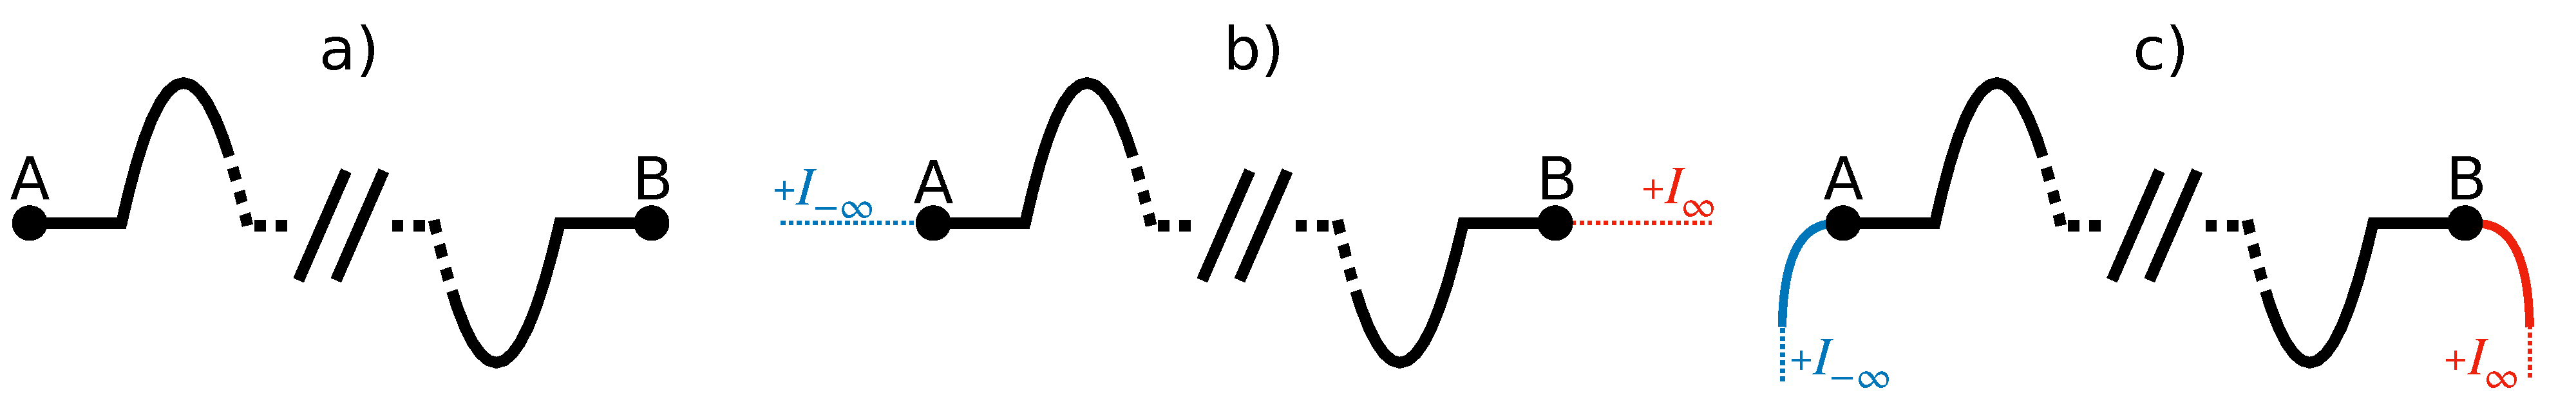
\includegraphics[width=0.95\linewidth]{content/images/5_THz_Source/integration_lim.pdf}
        \captionsetup{justification=centering}
        \caption{Schematic representation of the integration path over a magnetic structure. a) represents integration solely within the limits where the magnetic field is defined, i.e., from $A$ to $B$. b) shows the case when one semi-analytically estimates the contribution from the outer parts $[-\infty, A]$ and $[B, +\infty]$. c) represents a numerical trick on how to render this semi-analytical estimation negligible in codes where this estimation is performed automatically.}
        \label{Fig:integration_lim}
    \end{figure}
    
    One practical solution to this problem is to estimate these outer parts semi-analytically. The integral is split into three integration regions: $[-\infty, A]$, $[A, B]$, and $[B, +\infty]$, where $A$ and $B$ should be carefully chosen to avoid highly oscillatory behavior.
    \begin{align}
        \int_{-\infty}^{\infty} F e^{-i G} dz = \int_{-\infty}^{A} F e^{-i G} dz + \int_{A}^{B} F e^{-i G} dz + \int_{B}^{\infty} F e^{-i \omega G} dz
    \end{align}
    After performing a simple asymptotic integral expansion of the outer parts up to the second order, in accordance with a Filon-type method~\rr{cite}, one can obtain the follwing expression: \rr{correct formula}:
    \begin{align}
        \int_{-\infty}^{\infty} F e^{-i G} dz \approx \int_{A}^{B} F e^{-i G} dz + \bigg[ \cfrac{F}{i G'} + \cfrac{F'G' - FG''}{G'^3} e^{-i G}\bigg] \bigg |_{A}^{B}
        \label{Eq:integral_ev_semianalytical}
    \end{align}
    This semi-analytical estimation of the outer integral has not yet been incorporated into the developed code. This omission is partly due to the fact that, in the case of the general approach, one needs to first estimate the numerical derivatives, both first and second order, which can lead to a loss of accuracy and possible numerical artifacts, as well as demand careful implementation. For the sake of completeness in this presentation, I offer a comparison of the scenario where the contribution from the edges is not accounted for in \rr{the developed code}, against SRW, which can account for this contribution. This comparison is presented in Fig.~\ref{Fig:bend_edge_on}.
    \begin{figure*}[h!]
    	\centering
        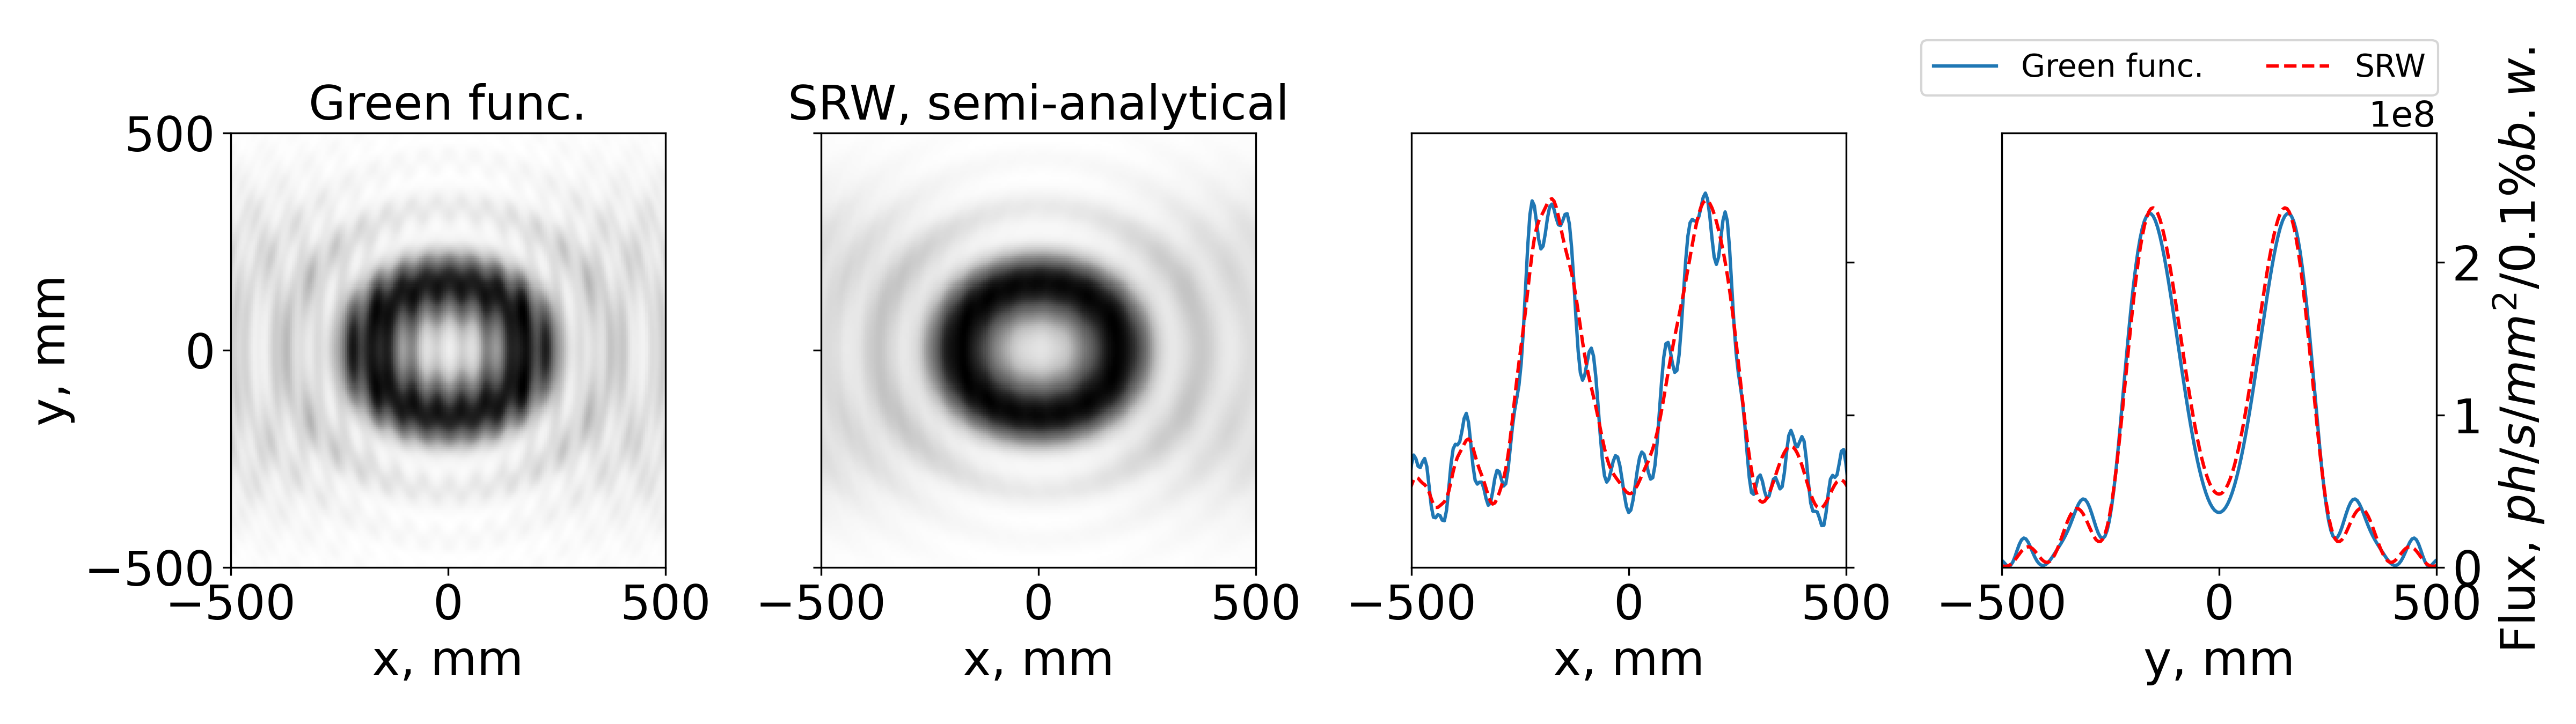
\includegraphics[width=0.95\linewidth]{content/images/5_THz_Source/bend_edge_on.png}
        \captionsetup{justification=centering}
        \caption{Comparison of computational results from \rr{the developed code} and SRW for the radiation from the magnetic structure presented in Fig.~\ref{Fig:bending_magnet} (arrangement of bending magnets). SRW accounts for the outer integral estimation, which is denoted in the corresponding figure as "SRW, semi-analytical". Total flux is presented for both polarization components.}
        \label{Fig:bend_edge_on}
    \end{figure*}
    
    Initially, I developed the code without being aware of this issue, and an evident incongruity in the results led to this in-depth cross-check. Thanks to a very productive discussion with E. Saldin and G. Geloni, who provided hints towards resolving this apparent paradox, and to the invaluable correspondence with O. Chubar, who explained the solution in more detail.
    
    In conducting cross-checks, it's crucial to recognize that other numerical codes might handle these terms differently. For instance, the formula is clearly implemented in the SRW code and, to the best of my knowledge, is tacitly applied in calculations within the SPECTRA and OCELOT toolkits. As mentioned, SRW allows for the semi-analytical estimation to be 'turned on' and 'off.' When set to 'off,' integration occurs only over the specified magnetic field from $A$ to $B$. In contrast, SPECTRA and OCELOT consistently account for this semi-analytical estimation, complicating cross-checks with \oo{the developed code}.~
    
    One way to overcome this issue is by adding instantaneous turns in the radiation trajectory at points $A$ and $B$ (e.g., via an abrupt magnetic field kick, as shown in Fig.~\ref{Fig:integration_lim}.(c)). This approach alters the estimation of the outer integrals, rendering their contribution negligible. Nonetheless, for a fair cross-check, it is sufficient to compare \rr{the developed} code with SRW only, since SPECTRA and OCELOT yield the same results as SRW when semi-analytical estimation is "on" and have been cross-checked against each other elsewhere \rr{cite}. Therefore, the cross-check will focus on the portion of the trajectory from $A$ to $B$, corresponding to the numerical case depicted in Fig.~\ref{Fig:integration_lim}.(a).
    
    Continuing the discussion, it is evident that there are two approaches to tackling the calculation of synchrotron radiation. The first approach involves defining a trajectory from $A$ to $B$, ensuring it is 'physical,' meaning the contribution from the edges is negligible. This method is the most straightforward but may lead to the emergence of highly oscillatory integrals, which require careful consideration. The second alternative involves semi-analytically evaluating the outer integral according to Eq.~\ref{Eq:integral_ev_semianalytical}. However, in this case, this estimation may not accurately represent the real magnetic configuration outside the defined range from $A$ to $B$, which can influence the resulting radiation distribution.

\subsubsection{Three pole radiation}
    In this subsection, I will present another numerical example featuring a three-pole device, as shown in Fig.~\ref{Fig:3pole_traj}. In this magnetic system, the first and the second magnetic field integrals are "closed", effectively returning the electron to $x, y = 0$ and $x_p, y_p = 0$. This makes the integrant to be zero, as illustrated in Fig.~\ref{Fig:3pole_traj}. Consequently, highly oscillatory behaviors are effectively suppressed, simplifying the integration process. However, this scenario is not entirely physical, as only part of the trajectory is defined. Thus, one can also observe the influence of the edge terms, evident in the characteristic interference circles depicted in Fig.~\ref{Fig:pole}. Nevertheless, this reinforces the cross-check as it represents a more challenging case to calculate
    \begin{figure*}[p]
        \centering
        \begin{subfigure}[c]{0.5\linewidth}  % [c] option for vertical centering
            \centering
            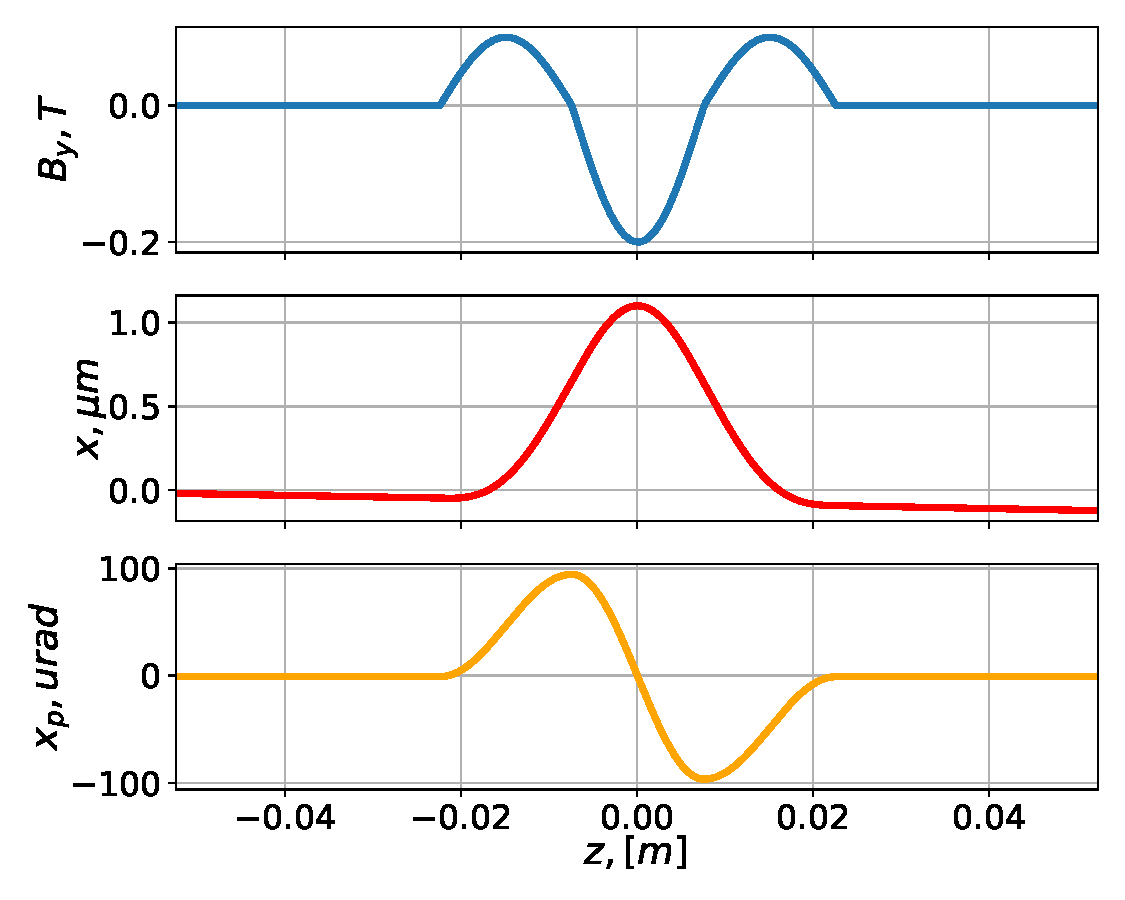
\includegraphics[width=\linewidth]{content/images/5_THz_Source/3pole_traj.pdf}
            \caption{From top to bottom: $y$ component of the magnetic field, $x$ component of the trajectory and $x_p$ is the angel of the electron's direction.} % Optional individual caption for the first subfigure
            \label{Fig:3pole_traj}
        \end{subfigure}%
        \begin{subfigure}[c]{0.5\linewidth}  % [c] option for vertical centering
            \centering
            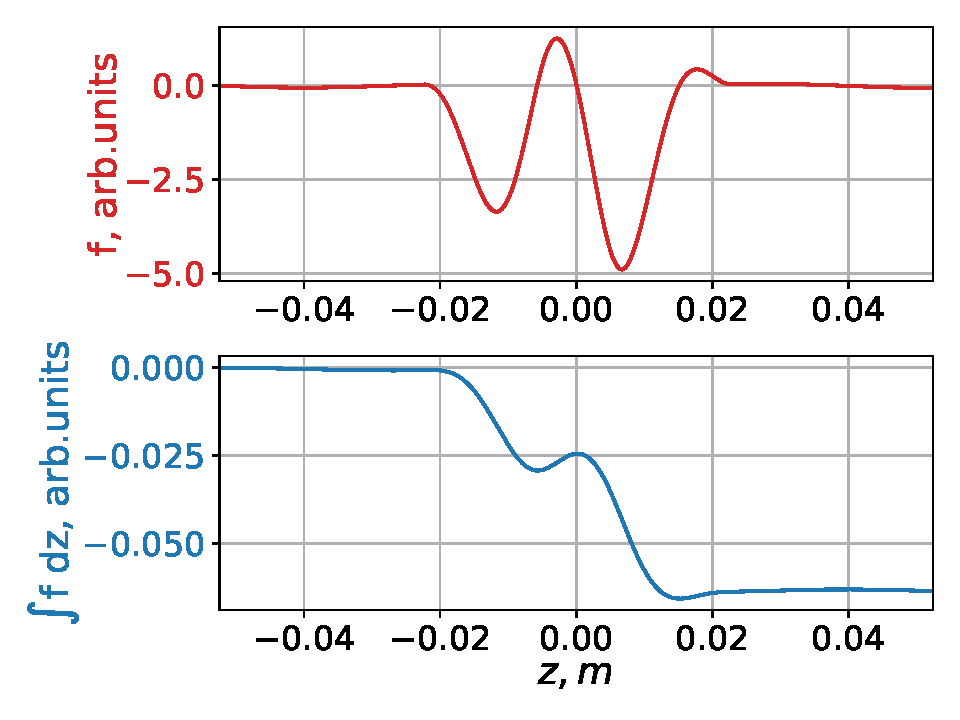
\includegraphics[width=\linewidth]{content/images/5_THz_Source/3pole_integral.pdf}
            \caption{Integrant value with respect to $z$ value and corresponding integral value for the three pole radiation.} % Optional individual caption for the second subfigure
            \label{Fig:3pole_integral}
        \end{subfigure}
        \caption{Three pole trajectory and integral evaluation with respect to the longitudinal coordinate.} % Optional overall caption            
        \label{Fig:3pole_figs}
    \end{figure*}
    
    \begin{figure*}[p]
    	\centering
        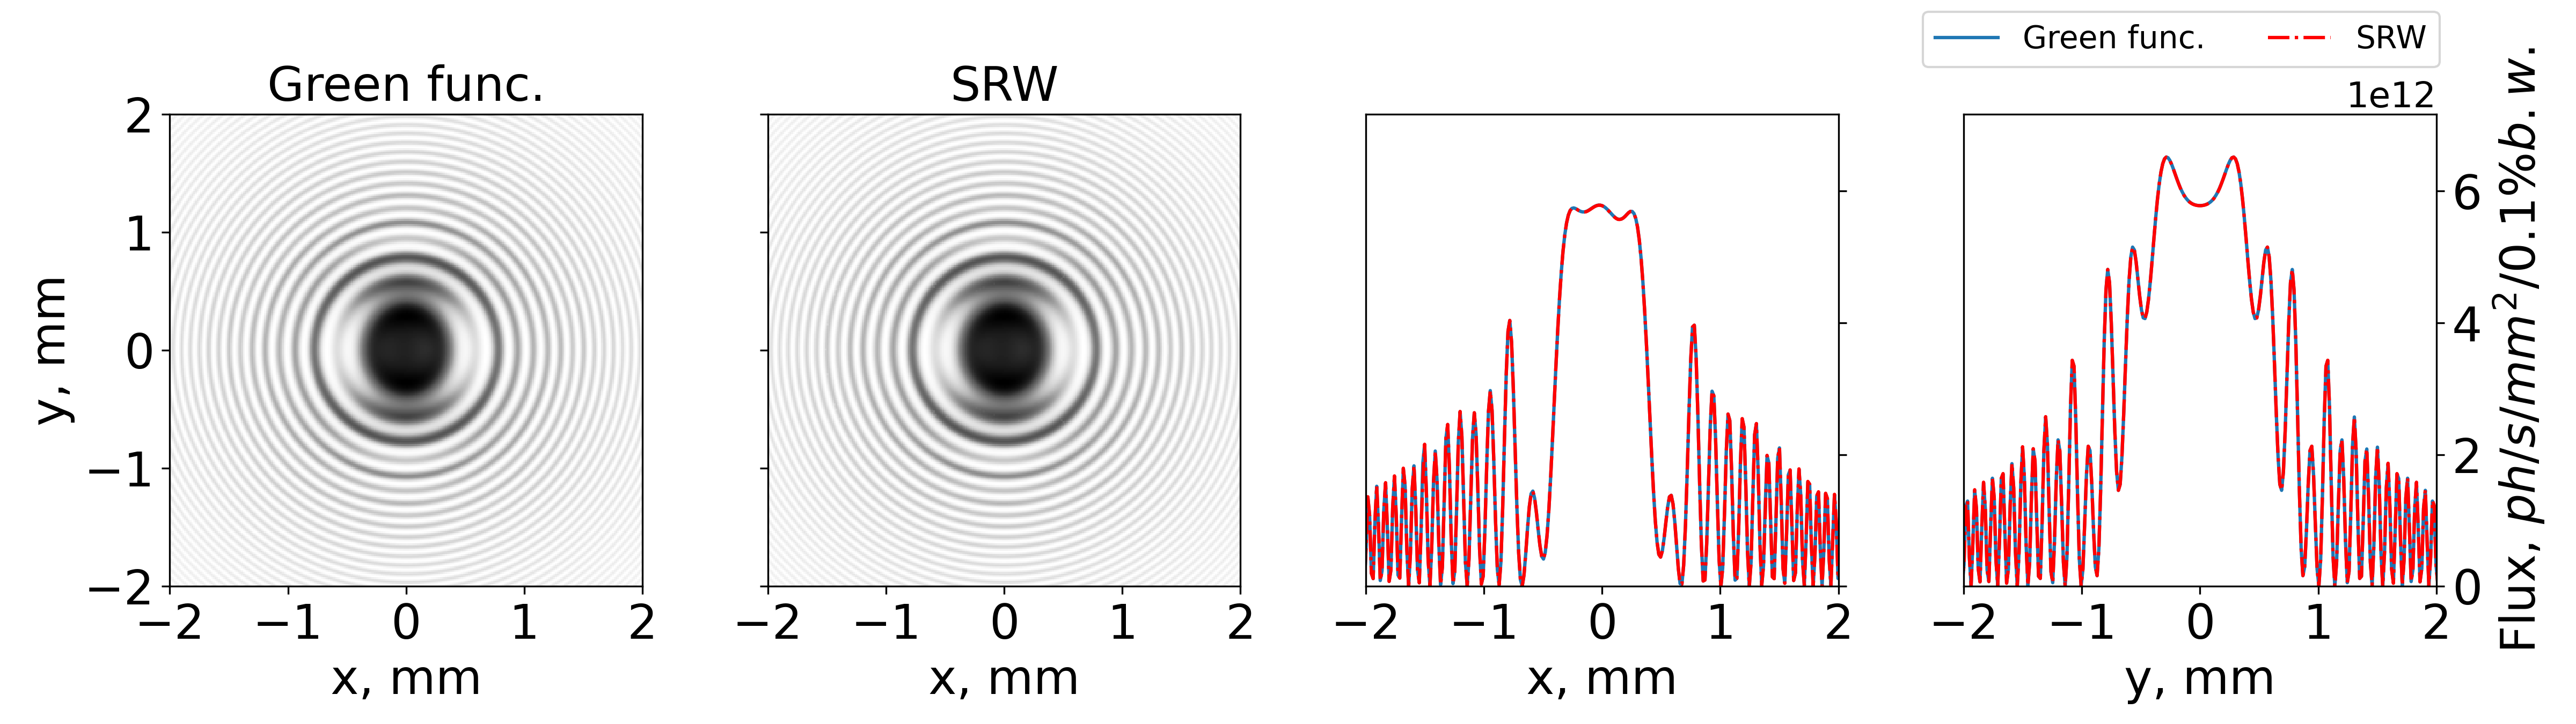
\includegraphics[width=0.95\linewidth]{content/images/5_THz_Source/3pole.png}
        \captionsetup{justification=centering}
        \caption{Comparison of computational results from \rr{the developed code} and SRW for the radiation from the magnetic structure presented in Fig.~\ref{Fig:pole} a three pole device.  Total flux is presented for both polarization components.}
        \label{Fig:pole}
    \end{figure*}

\subsubsection{Undulator radiation radiation}
    Another case that should be checked is undulator radiation, for example, from a magnetic field seen in Fig.~\ref{Fig:und_traj}. In undulators, the integral value adds up 'coherently' at each period (Fig.~\ref{Fig:und_integral}). This is essentially the unique property of undulator radiation that increases the power of radiation compared to a single pole, in proportion to the square of the number of undulator periods. In cases where the influence of the edge terms is barely noticeable on the total power distribution of the radiation in resonance (Fig.~\ref{Fig:und}), it is because the radiation from the device is an order of magnitude higher than that from the edges. However, it can be clearly seen for the $y$ polarization component, as depicted in Fig.~\ref{Fig:und_edge_on}. I need to note that to calculate the last case with SRW, it was necessary to add small straight sections before and after the undulator to proceed correctly with the semi-analytical estimation overwise it gives numerical artefacts.
    
    \begin{figure*}[p]
        \centering
        \begin{subfigure}[c]{0.5\linewidth}  % Use [c] for vertical centering
            \centering
            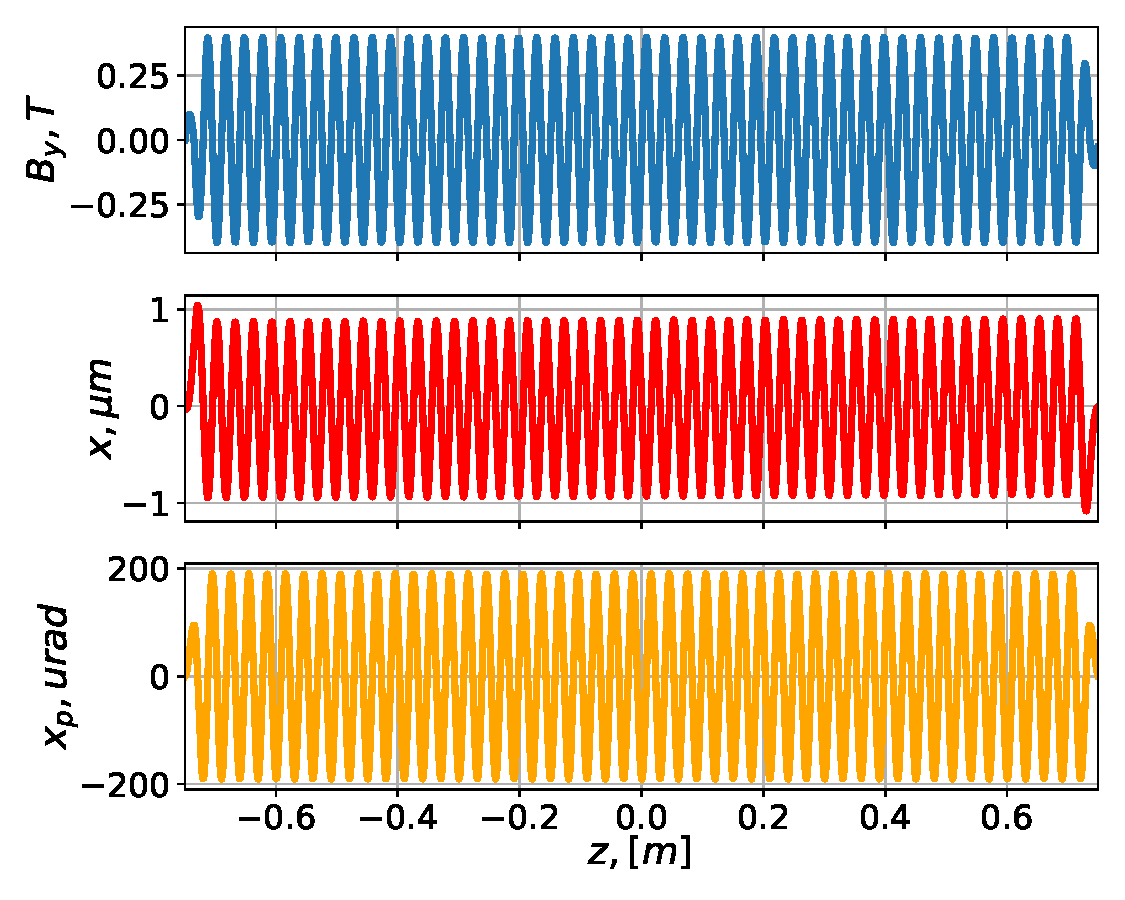
\includegraphics[width=\linewidth]{content/images/5_THz_Source/und_traj.pdf}
            \caption{From top to bottom: $y$ component of the magnetic field, $x$ component of the trajectory and $x_p$ is the angel of the electron's direction.} % Optional individual caption for the first subfigure
            \label{Fig:und_traj}
        \end{subfigure}%
        \begin{subfigure}[c]{0.5\linewidth}  % Use [c] for vertical centering
            \centering
            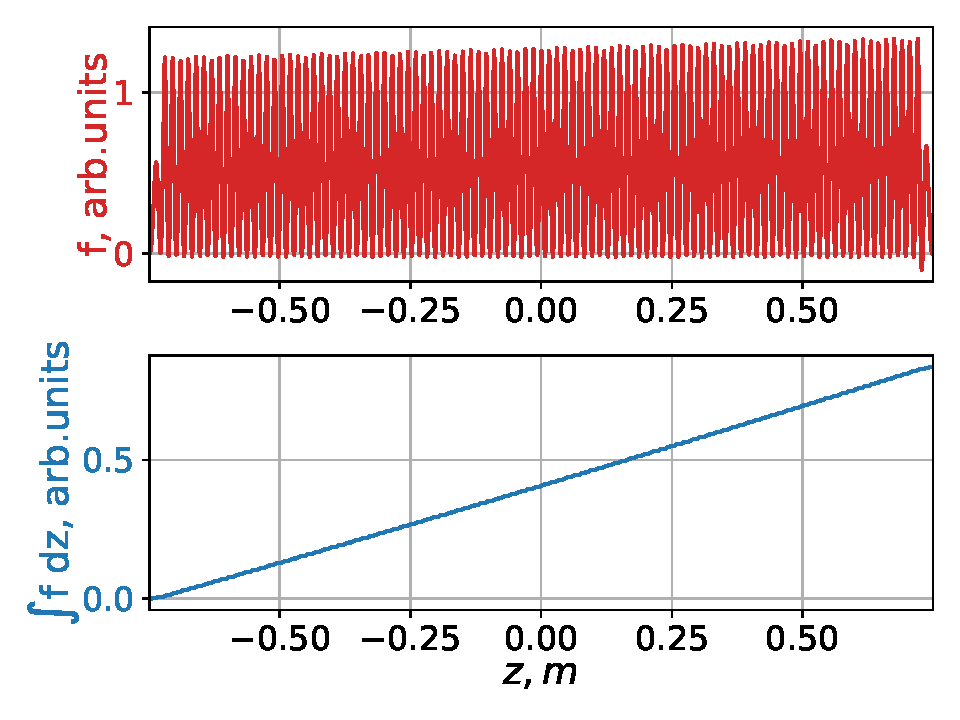
\includegraphics[width=\linewidth]{content/images/5_THz_Source/und_integral.pdf}
            \caption{Integrant value with respect to $z$ value and corresponding integral value for the undulator radiation.} % Optional individual caption for the second subfigure
            \label{Fig:und_integral}
        \end{subfigure}
            \caption{Undulator trajectory and integral evaluation with respect to the longitudinal coordinate.} % Optional overall caption            \label{fig:three_pole_figures}        \label{fig:und_figures}
        \label{Fig:und_integral_and_traj}
    \end{figure*}

    \begin{figure*}[p]
    	\centering
        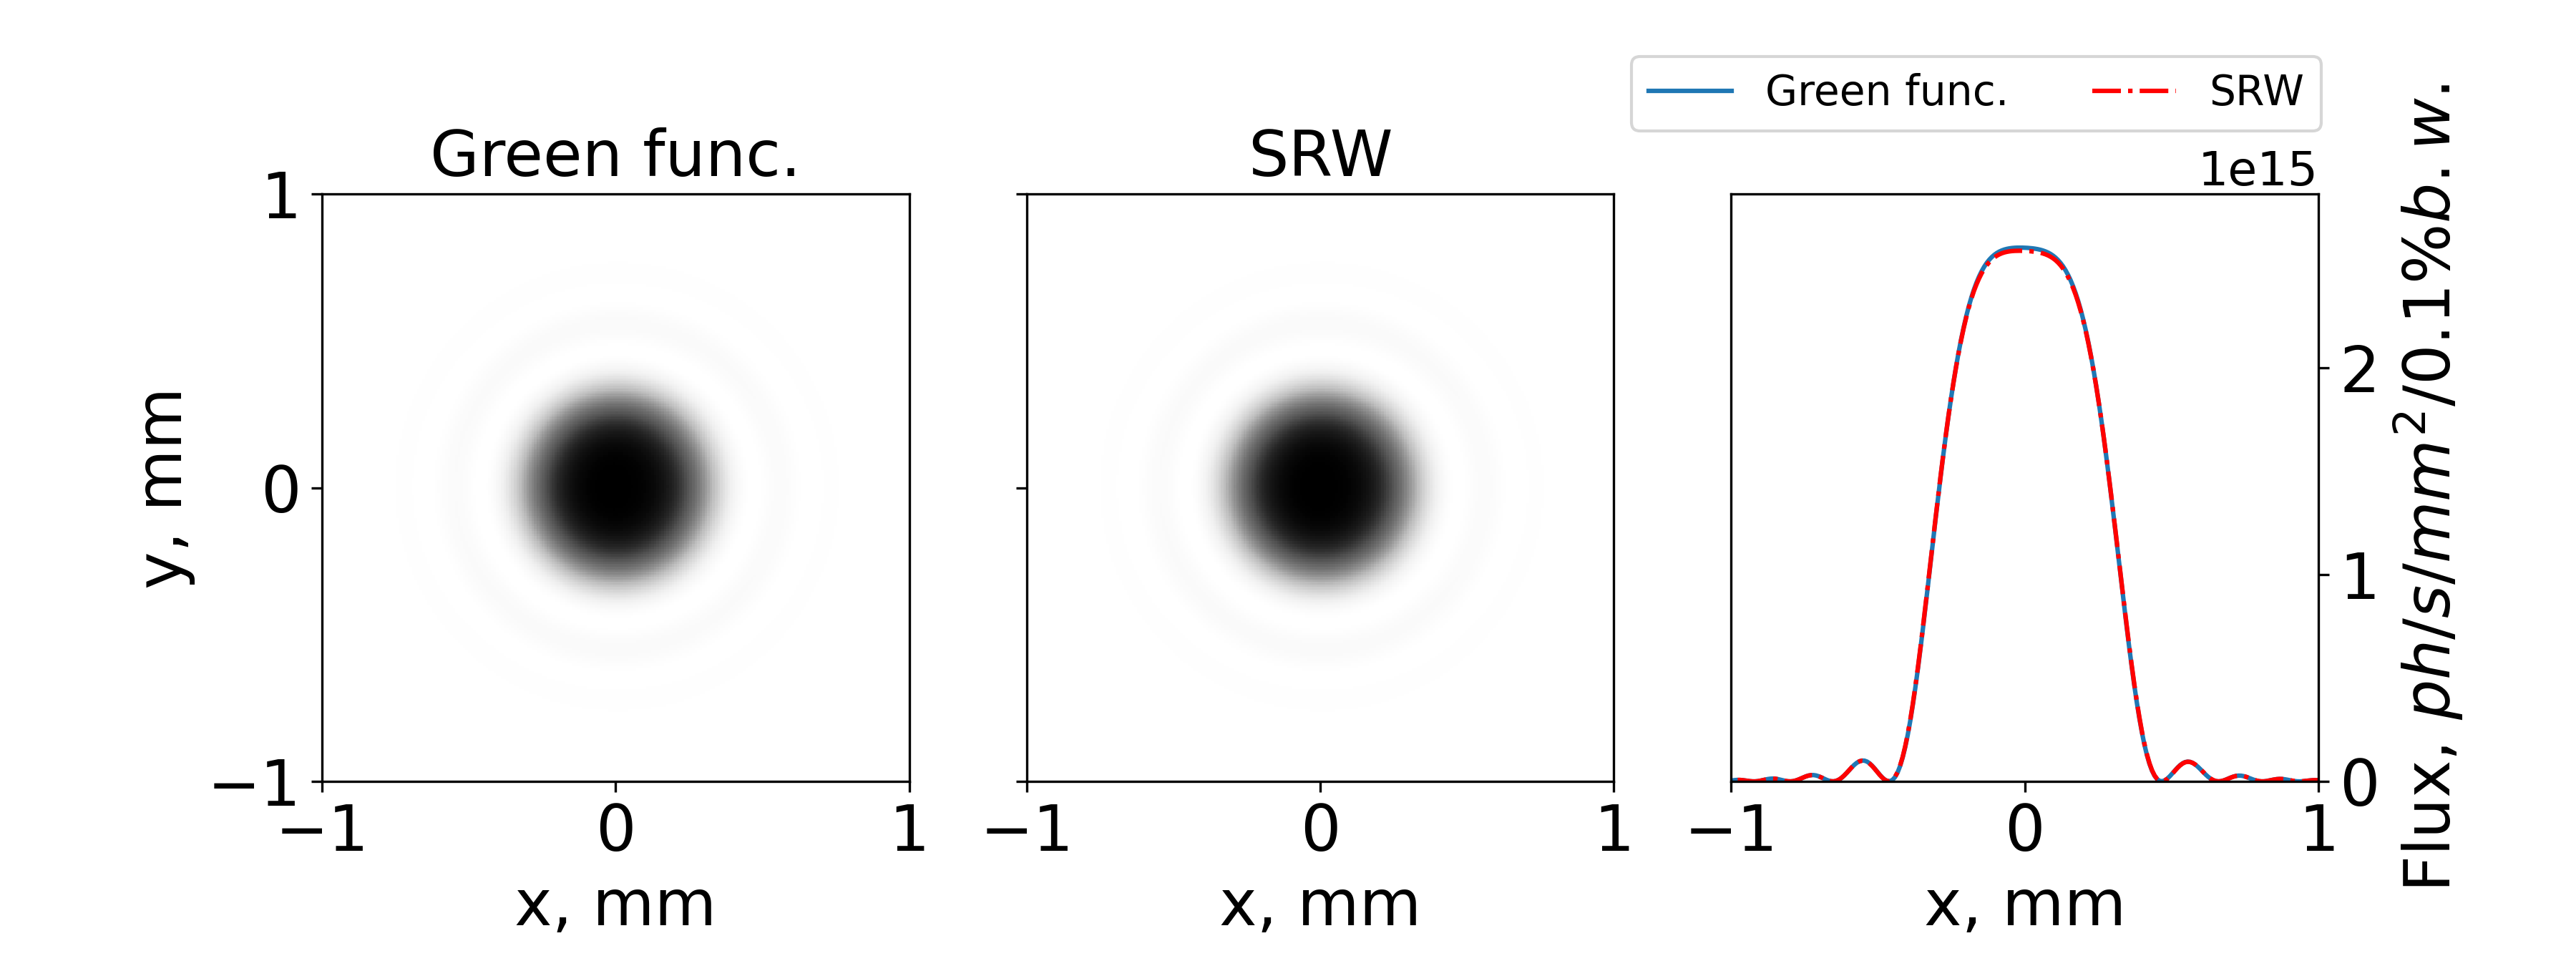
\includegraphics[width=0.71\linewidth]{content/images/5_THz_Source/und.png}
        \captionsetup{justification=centering}
        \caption{Comparison of computational result from different codes of radiation from the undulator radiation. Total flux is presented for both polarization components.}
        \label{Fig:und}
    \end{figure*}

    \begin{figure*}[p]
    	\centering
        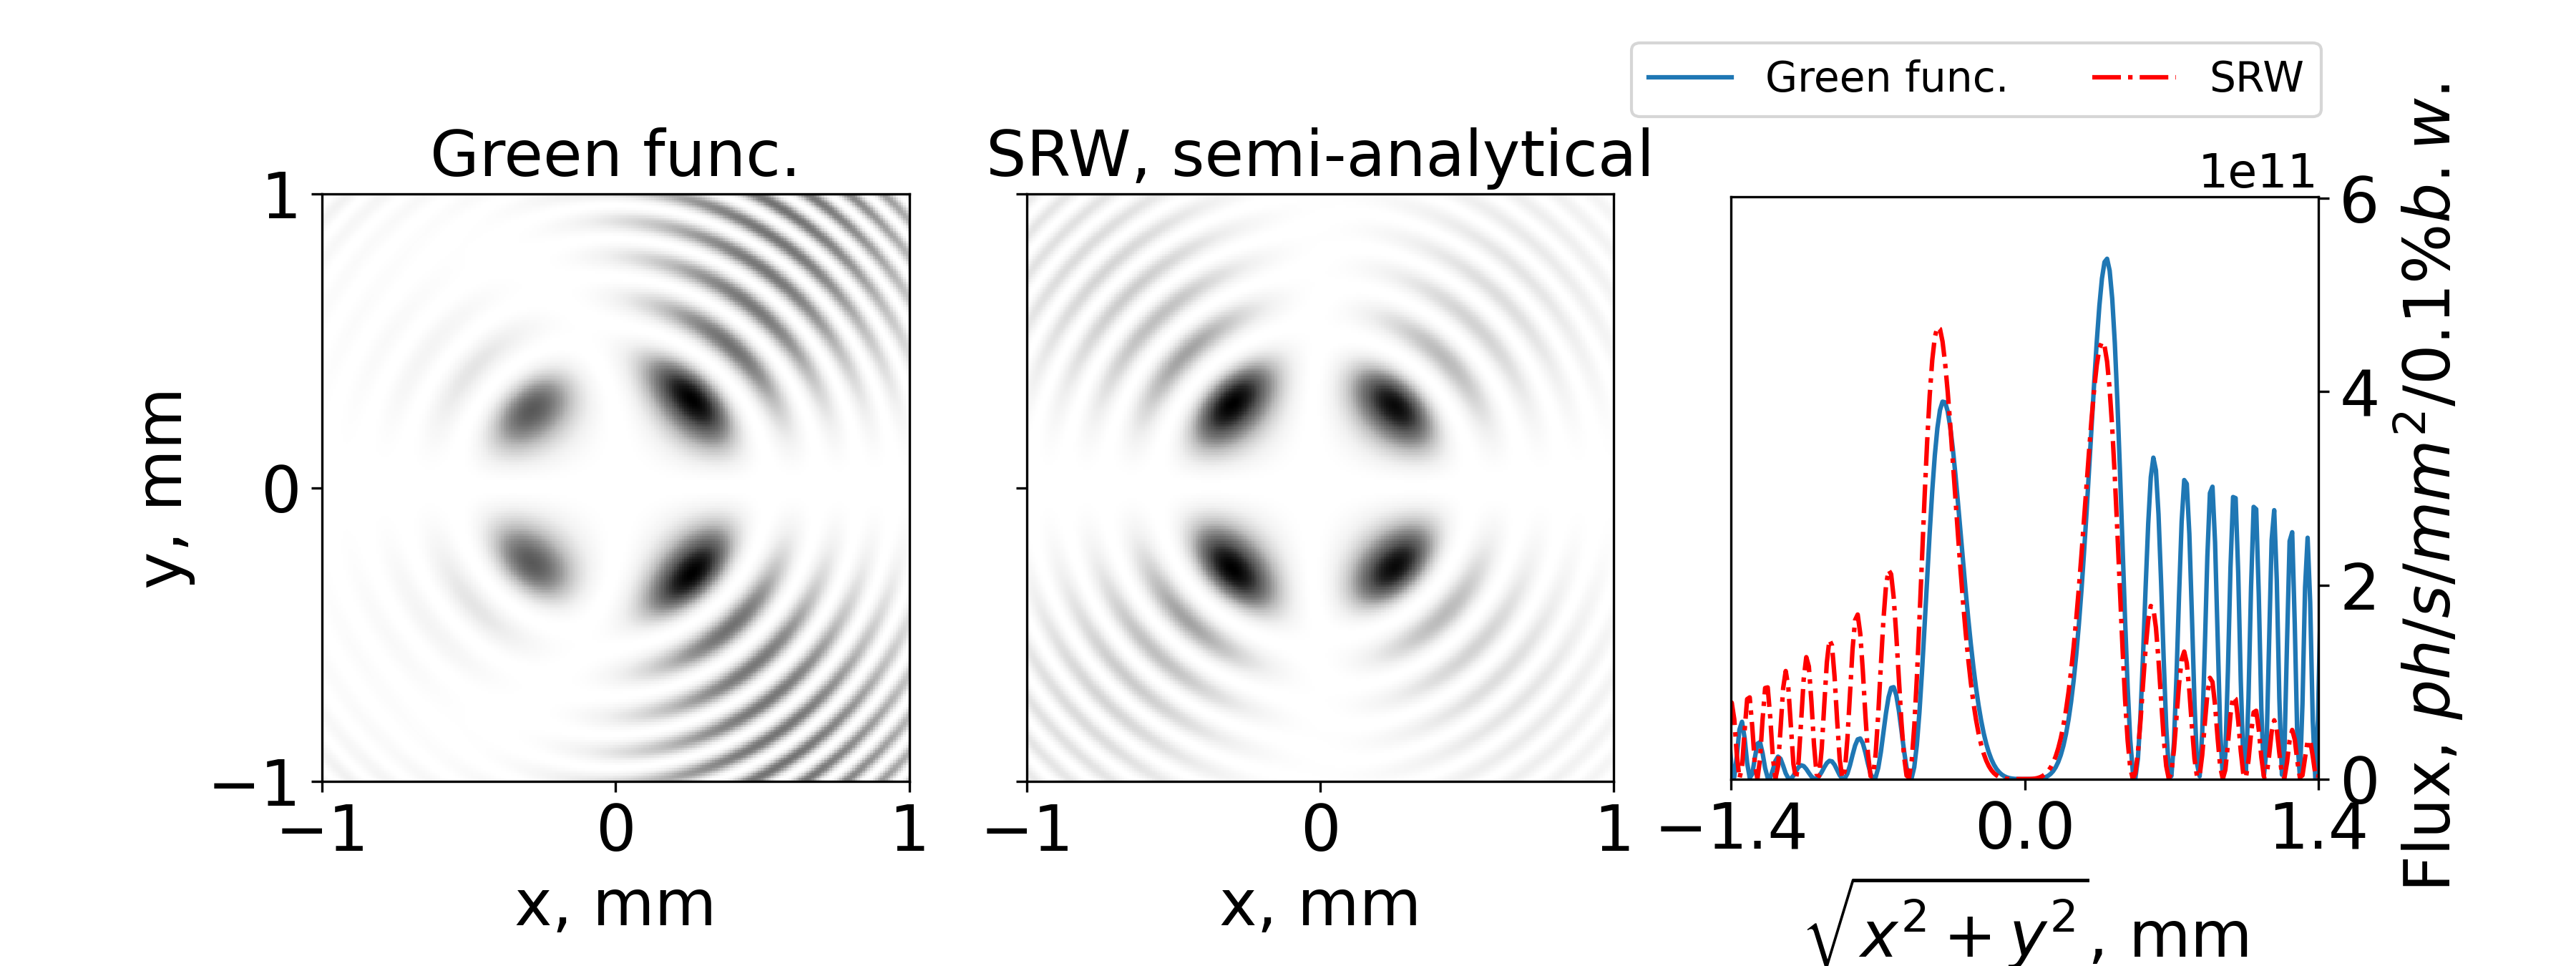
\includegraphics[width=0.71\linewidth]{content/images/5_THz_Source/und_edge_on.png}
        \captionsetup{justification=centering}
        \caption{Comparison of computational result from different codes of radiation from the undulator radiation. y-polarization flux is presented. The slice on the right subplot is presented for the diagonal cut.}
        \label{Fig:und_edge_on}
    \end{figure*}
    \pagebreak
    
\subsubsection{Straight section}
    I would like to conclude this section with the case of radiation from a straight section to demonstrate the contribution from the edges that I observed in the previous examples. By "straight section", I mean that the electron is created at point $A$, flies to $B$ in space with no magnetic field, and then disappears at $B$. This case represents radiation from two point sources situated at $A$ and $B$ and is described by the expression:   
    \begin{align}
        \vec{\widetilde{E}}_{AB}=\frac{ i \omega e L}{c^2 z}
        \exp\left[\frac{i \omega \theta^2 z}{2 c}\right] \vec{\theta} ~
        \mathrm{sinc}\left[\frac{\omega L}{4
        c}\left(\theta^2+\frac{1}{\gamma^2}\right)\right].
        \label{Eq:AB_analytical}    
    \end{align}
   Alternatively, this radiation can be understood using the integral expression where the sole contribution is from the 'gradient' term. I have depicted the cross-check of this case with SRW and the analytical expression in Eq.\ref{Eq:AB_analytical} in Fig.\ref{Fig:AB}.
    \begin{figure*}[h!]
    	\centering
        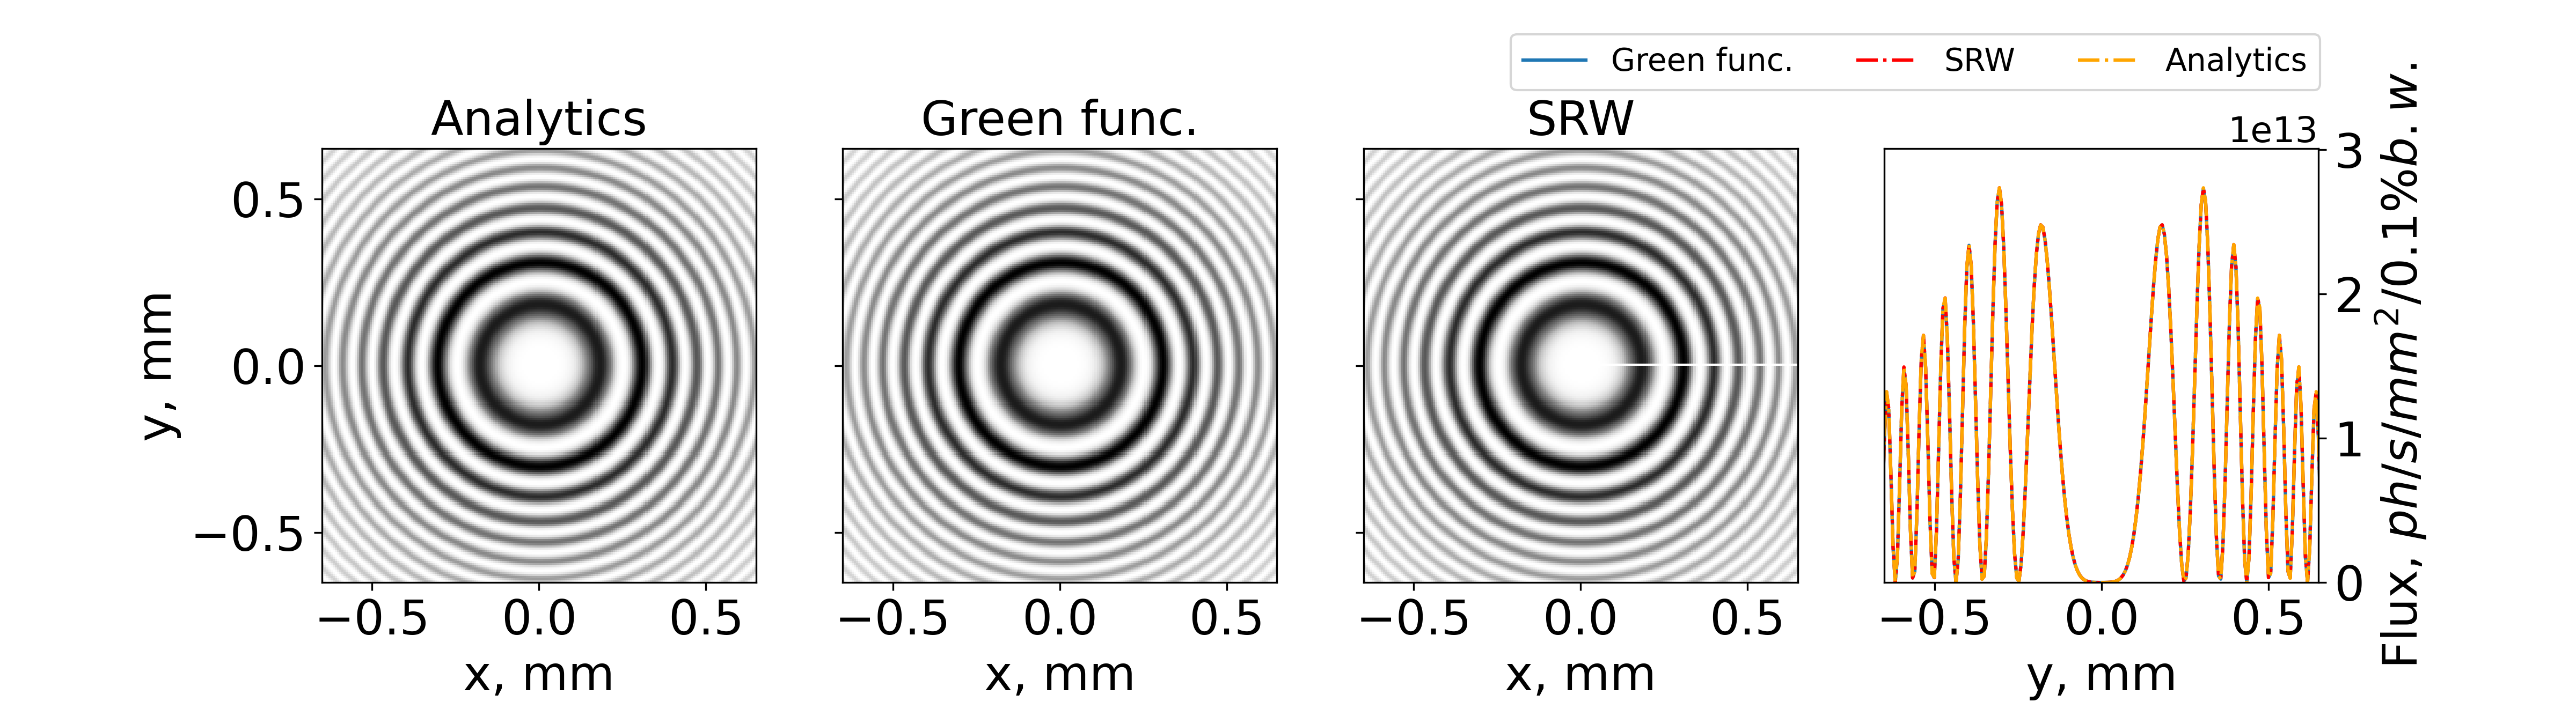
\includegraphics[width=0.99\linewidth]{content/images/5_THz_Source/AB.png}
        \captionsetup{justification=centering}
        \caption{Comparison of computational result from different codes of radiation from a straight section.}
        \label{Fig:AB}
    \end{figure*}
    
    These cases I have presented in this section demonstrate the applicability of the chosen approach of an integrator that can accept a Green function as input and perform integration (as well as taking derivatives from the Green's function). For this case of the free space Green's function, it has shown certain robustness in calculating the 'gradient' term. The next step in these cross-checks is to calculate examples using the circular waveguide Green's function.
    
\subsection{Circular waveguide Green's function}
    In this section I will present the result of the calculations using the circular waveguide Green's function and the cross-check of this results with asymptotic and analytical expressions. 

    The author of \rr{cite} represent the Green's function for the circular waveguide in the following form:
    \begin{eqnarray}
        &&G\left(\vec{r}_\bot,\vec{r'}_\bot,z-z'\right) = \frac{c}{2 i
        \omega} \sum_{m=0}^{\infty}\sum_{k=1}^{\infty}
        \left(A^{TE}_{mk}\right)^2 \left(\frac{\mu_{mk}}{2 R }\right)^2
        \exp\left[-\frac{i c (z-z')}{2\omega R^2 } \mu_{mk}^2\right] \cr
        && \times \left\{\left[\begin{array}{c} J_{m-1}(\mu_{mk}r/R)
        \cos[(m-1)\phi]+J_{m+1}(\mu_{mk}r/R) \cos[(m+1)\phi]
        \\
        -J_{m-1}(\mu_{mk}r/R) \sin[(m-1)\phi]+J_{m+1}(\mu_{mk}r/R)
        \sin[(m+1)\phi]
        \end{array}\right] \right. \cr && \left. \otimes \left[\begin{array}{c} J_{m-1}(\mu_{mk}r'/R)
        \cos[(m-1)\phi']+J_{m+1}(\mu_{mk}r'/R) \cos[(m+1)\phi']
        \\
        -J_{m-1}(\mu_{mk}r'/R) \sin[(m-1)\phi']+J_{m+1}(\mu_{mk}r'/R)
        \sin[(m+1)\phi']
        \end{array}\right] \right. \cr && \left. +
        \left[\begin{array}{c} -J_{m-1}(\mu_{mk}r/R)
        \sin[(m-1)\phi]-J_{m+1}(\mu_{mk}r/R) \sin[(m+1)\phi]
        \\
        -J_{m-1}(\mu_{mk}r/R) \cos[(m-1)\phi]+J_{m+1}(\mu_{mk}r/R)
        \cos[(m+1)\phi]
        \end{array}\right] \right. \cr && \left. \otimes
        \left[\begin{array}{c} -J_{m-1}(\mu_{mk}r'/R)
        \sin[(m-1)\phi']-J_{m+1}(\mu_{mk}r'/R) \sin[(m+1)\phi']
        \\
        -J_{m-1}(\mu_{mk}r'/R) \cos[(m-1)\phi']+J_{m+1}(\mu_{mk}r'/R)
        \cos[(m+1)\phi']
        \end{array}\right]\right\}
        \cr && + \frac{c}{2 i \omega}
        \sum_{m=0}^{\infty}\sum_{k=1}^{\infty} \left(A^{TM}_{mk}\right)^2
        \left(\frac{\nu_{mk}}{2 R }\right)^2 \exp\left[-\frac{i c
        (z-z')}{2\omega R^2 } \nu_{mk}^2\right] \cr && \times
        \left\{\left[\begin{array}{c} J_{m-1}(\nu_{mk}r/R)
        \sin[(m-1)\phi]-J_{m+1}(\nu_{mk}r/R) \sin[(m+1)\phi]
        \\
        J_{m-1}(\nu_{mk}r/R) \cos[(m-1)\phi]+J_{m+1}(\nu_{mk}r/R)
        \cos[(m+1)\phi]
        \end{array}\right] \right. \cr && \left. \otimes \left[\begin{array}{c} J_{m-1}(\nu_{mk}r'/R)
        \sin[(m-1)\phi']-J_{m+1}(\nu_{mk}r'/R) \sin[(m+1)\phi']
        \\
        J_{m-1}(\nu_{mk}r'/R) \cos[(m-1)\phi']+J_{m+1}(\nu_{mk}r'/R)
        \cos[(m+1)\phi']
        \end{array}\right] \right. \cr && \left. +
        \left[\begin{array}{c} J_{m-1}(\nu_{mk}r/R)
        \cos[(m-1)\phi]-J_{m+1}(\nu_{mk}r/R) \cos[(m+1)\phi]
        \\
        -J_{m-1}(\nu_{mk}r/R) \sin[(m-1)\phi]-J_{m+1}(\nu_{mk}r/R)
        \sin[(m+1)\phi]
        \end{array}\right] \right. \cr && \left. \otimes
        \left[\begin{array}{c} J_{m-1}(\nu_{mk}r'/R)
        \cos[(m-1)\phi']-J_{m+1}(\nu_{mk}r'/R) \cos[(m+1)\phi']
        \\
        -J_{m-1}(\nu_{mk}r'/R) \sin[(m-1)\phi']-J_{m+1}(\nu_{mk}r'/R)
        \sin[(m+1)\phi']
        \end{array}\right]\right\}~.
        \label{Eq:Circular_waveguide_green_function}
    \end{eqnarray}
    This expression should be substituted in Eq.~\ref{Eq:field_integral_tensor_full}. The first one and quite natural numerical cross-check is to let the radius of the waveguide be large and compare the result with the case of the free space Green function. 

\subsubsection{Free space limit}
    The next cross-check involves comparing the calculation results when the radius of the waveguide is large ($R = 1$~m). A radius of $1$~m, rather than a larger size, was chosen based on the reasoning that a larger radius would result in different transverse mode content and an increased number of $k$ modes that require summation. The selected radius of $1$~m is deemed sufficient for a demonstrative cross-check. One would expect that the radiation with the waveguide Green's function should result in the same spectral distribution as the free space Green function in the limit of large radius. For this calculation, I chose to use a three-pole device (a phase shifter), with the length of a pole being $0.45$~m and the magnetic field of the central pole at $2$~T and the side poles at $1$~T. I calculated spectral flux distribution and the result of the cross-check is presented in Fig.~\ref{Fig:free_space_limit}. 
    \begin{figure*}[h]
    	\centering
        \includegraphics[width=0.8\linewidth]{content/images/5_THz_Source/free_space_limit.pdf}
        \captionsetup{justification=centering}
        \caption{The on-axis spectral flux from a three-pole device was calculated using the free space Green's function (represented by the black solid line) and the circular waveguide Green's function, taking into account different amounts of transverse modes: a blue dash-dotted line for 1000 modes and a dashed line for 1500 modes.}
        \label{Fig:free_space_limit}
    \end{figure*}
    
    The presented distribution can be divided into three parts. At the low end of radiation frequencies, there is a mismatch that can be explained by the appearance of highly oscillatory integrals. As one calculates higher mode number contributions, one can see that the exponent's argument starts to grow as well, along with $\mu_{mk}$ and $\nu_{mk}$. Then, there is a region where the two lines coincide — the behavior one would expect. Additionally, one observes an oscillatory behavior that indicates more modes should be summed, as can be seen when comparing the blue dashed-dotted line with the orange dashed line.

    It is relatively easy to cross-check on-axis spectral flux distributions because all transverse modes with a number higher than $m=1$ are equal to zero, as evidenced by the expression for the Green's function. This significantly simplifies the cross-check process, but it is still necessary to verify as general a case as possible. In the next section, I will present a cross-check of a real-sized waveguide against the analytical derivation that was made in~\rr{cite}.
    
\subsubsection{Spatial distribution}
    For this cross-check I chose an undulator with ten periods, the period length is $0.9$~m and the max magnetic field value is $2$~T. The magnetic field distribution does not have any end correction coils. This is made for the fair comparison as the analytical distribution is calculated for an idealized sin-like field distribution. I present this comparison in Fig.~\ref{Fig:pipe_check_2D} and the cross-section in Fig.~\ref{Fig:pipe_check_1D}.
    \begin{figure*}[p]
    	\centering
        \includegraphics[width=0.99\linewidth]{content/images/5_THz_Source/pipe_check_2D.png}
        \captionsetup{justification=centering}
        \caption{Spatial distribution of radiation in the far zone from a ten period undulator in a waveguide.}
        \label{Fig:pipe_check_2D}
    \end{figure*}
    \begin{figure*}[p]
    	\centering
        \includegraphics[width=0.99\linewidth]{content/images/5_THz_Source/pipe_check_1D.png}
        \captionsetup{justification=centering}
        \caption{Cross sections of the spatial distribution shown in Fig.~\ref{Fig:pipe_check_2D}.}
        \label{Fig:pipe_check_1D}
    \end{figure*}

    In the cross-check I show only $k=1$, other modes coincides reasonably well resulting in a more complex spatial distribution. I believe this representation is enough for a fair cross-check and more studies should be done on physical interpretation of the the computational results, which definitely should be a subject for future work.
    
\section{Discussion and outlook}
    
    The developed code is valuable for calculating insertion devices in physics situations where the influence of metallic components is substantial on the radiation. For example, this applies to applications like THz undulator sources for beamlines at FEL facilities. For these facilities, it is crucial to know the source characteristics well in order to optimize the subsequent propagation system.

    As of the moment of writing these lines (April 2024), the code has several weak points in terms of numerical efficiency. Initially written as a simple Python script to test the idea of writing the code for an arbitrary Green's function, it utilizes static memory allocation—multidimensional arrays are defined before running the code, which under certain circumstances leads to RAM overloads. Moreover, this implementation is not suitable for wrapping the code in faster programming languages like C. Numerical efficiency will need to be improved in the next releases of the code.

[[[GG ARRIVED HERE]]]
\chapter{Iris wave guide for THz radiation transport}

    \section{Introduction}
    Incorporating a THz source at the European XFEL facility, utilizing a spent beam, would necessitate propagating the THz radiation from the location of the beam dump at XHE4/XS4 to the experimental hall of the users' end stations in XHQ, a distance estimated to be 370 meters, as seen in Fig.~\ref{Fig:transport outline}. Propagation of THz radiation over such a long distance imposes significant challenges, especially if the transmission system is required to accept a broadband of frequencies, spanning from $3$ to $30$ THz or even broader, down to $0.3$ THz.
    
    \begin{figure*}[h!]
    	\centering
    		\includegraphics[width=0.99\linewidth]{content/images/transport/aerial_view.pdf}
    		\centering
            \captionsetup{justification=centering}
        	\caption{Aerial view on the European XFEL campus with marking location of XHE4/XS4 and the users' hall in XHQ, the distance between them is measured to be $370$~m. In the call-out the scheme of XHE4/XS4 building at the UG2 level with outlined path of THz radiation through radiation protection maze. The diagnostic table is marked with a cyan blue rectangle}
        \label{Fig:transport outline}
    \end{figure*}
    
    THz radiation is highly absorbed by media and it is essential to avoid usage of any refractive optic elements, including filters and windows. To guide THz radiation one can consider using reflective optics or waveguides adjusted for the THz radiation range. The first approach, using reflective optics, is very suitable for complex tunnel geometries where one needs to guide radiation around corners. In contrast, waveguides are naturally suited to straight sections. In the THz radiation propagation beamline at the European XFEL, we plan to use both approaches: initial outcoupling occurs in XHE4/XS4, where radiation should be delivered to the XTD8 tunnel through a concrete radiation protection maze by means of a mirror-based system as illustrated in  the call-out in Fig.~\ref{Fig:transport outline}. And then we plan to deliver THz radiation through a $370$-meter-long XTD8 tunnel using a waveguide.
    
    In this chapter, we first provide an analysis of the THz radiation waveguide performance. We present two approaches to estimate its performance: one based on numerical simulation and the other using an analytical solution derived from complex boundary conditions. We calculate the efficiency of propagation of the fundamental mode of this waveguide and demonstrate the matching conditions for the incoming radiation. Additionally, we analyze the effects of imperfections on the waveguide's performance. Secondly, we outline the mirror-based propagation line and introduce a 'matching' device that ensures efficient coupling of the radiation from the source and the initial mirror system to the iris line.
    
    %\rr{discuss more about pros and cons of } Both approaches — one based on optical mirrors and the other on the iris line — have their advantages and limitations, and several considerations should be assessed before choosing one over the other. Mirrors offer a specific advantage in terms of achromaticity, allowing a mirror guide to be used across a wide range of frequencies. However, guiding a beam in a mirror system requires constant refocusing. The spacing between each refocusing section, which keeps the beam parallel, must be estimated by considering the Rayleigh length of the radiation to prevent divergence, as well as potential misalignment in the mirror setup. Large spacing may lead to significant deviations from the optical axis. Another consideration is the 45° incidence angle of the radiation on the mirrors, which means that a mirror-based system does not follow a straight line. In contrast, an iris line is inherently straight unless a bend is required, which can be achieved by inserting a plane mirror in the waveguide. The iris line also benefits from relatively low losses, around 10 \% per 100 meters of propagation, and is fairly tolerant to misalignment of the apertures, up to a scale of 1 mm. 

\section{Iris line theory}

    A waveguide for THz radiation consists of metallic screens with centered holes, as depicted in Fig.\ref{Fig:iris_mirror} (a). The 'virtual' side surface created by the screens effectively acts as a waveguide in the usual sense. We refer to this device as an iris line or an iris waveguide. The iris line actually bridges the gap between radio electronics and optics as it mixes the properties of usual waveguides using the theory of physical optics. The analysis of the electromagnetic field distribution in the iris line was first conducted using a numerical approach by Fox and Li\rr{cite}, followed by an analytical solution provided by Vainstein. Vainstein introduced complex boundary conditions at this virtual surface of the screen openings and derived the explicit expression of the iris line eigenmodes. Later, it was proposed~\rr{cite} to apply the iris line for THz radiation transportation at FEL facilities. The authors of~\rr{cite} present a comparative theoretical analysis of the iris line based on the theories of Fox and Li, and Vainstein, in application to the design of the transportation line. In this section, we extend the numerical approach further using an even simpler simulation approach that allowed us to account for the iris line imperfections. We also cross-checked our simulation results of the ideal iris line with the predictions given by Vainstein's theory and found excellent agreement.
    
    \begin{figure*}[h!]
    	\centering
    	% Answer: [trim={left bottom right top},clip]
    		\includegraphics[ width=0.79\linewidth]{content/images/transport/iris_mirror.pdf}
    		\centering
            \captionsetup{justification=centering}
        	\caption{Iris line and mirrors system outlines. Iris line has two main parameters: $a$ is the radius of the hole and $b$ is spacing between screens.}
        \label{Fig:iris_mirror}
    \end{figure*}
    
    As we mention, Fox and Li utilize a more numerical approach to finding the field distribution after radiation propagates through the iris line. This approach relies on the derivation of a radiation 'propagator' using physics optics. This implies that the iris line is essentially treated as a diffraction device, as depicted in Fig.~\ref{Fig:difraction_outline}. The first observation is that radiation incident on each screen will be partially diffracted back inside the virtual waveguide and partially inside the space between the screens. The latter portion of radiation will be reflected several times and will eventually be lost between two screens and does not affect the virtual waveguide. Therefore, Fox and Li made the primary approximation that the screen can be considered fully absorbing. 
    
    The second observation is that the problem can indeed be converted to the problem of radiation diffraction at an aperture. In this case, the Fresnel number is the only dimensionless parameter needed to describe the problem: $N = a^2 / (\lambda b)$, where $a$ is the radius of the opening of the iris line screens, $b$ is the spacing between screens, and $\lambda$ is the radiation wavelength. Comparing the approaches of Fox and Li and Vainstein's approach, one can see that namely, $N$ describes the transmission efficiency of the iris line, which we will show later in this section. For our simulations, we implemented the simplified Fox and Li approach. We propagate radiation in free space from the location of the $n$-th screen to the $(n+1)$-th screen and then apply a fully absorbing aperture, after which we repeat the propagation procedure again for the next cell.
    \begin{figure}[h!]
    	\centering
    		\includegraphics[trim={0 5cm 0 0cm}, width=0.75\linewidth]{content/images/transport/difraction_outline.jpeg}
    		\centering
            \captionsetup{justification=centering}
        	\caption{Iris line and mirrors system outlines}
        \label{Fig:difraction_outline}
    \end{figure}
    
    The approach developed by Vainstein, is mathematically robust and addresses the problem by taking into account the boundary conditions of the metallic walls and screens of the iris line: 
    
    \begin{align}
        \left[\vec{\widetilde{E}}+ (1+i) \beta_0 \sqrt{c b/(4 \omega)} ~
        (\vec{n} \cdot \vec{\nabla}_\bot) \vec{\widetilde{E}}\right]_{S} =
        0, 
        \label{Eq:Vainstein}
    \end{align}
    
    where $S$ is the virtual surface formed by the screens of the iris line, and
    $\vec{n}$ is the unit vector normal to $S$, $\beta_0 = 0.824$, $c$ is the speed of light, $\omega$ is the radiation frequency and $\widetilde{E}(r,\phi,z)$ is the amplitude.

    We seek the solution for the field amplitude, $\widetilde{E}(r,\phi,z)$, in the following form:
    
    \begin{align}
        \widetilde{E} = u_{nj}(r)\exp[-in \phi -i k_z z]~, \label{solu}
    \end{align}

    where $n = 0,1, 2, ...$ and $u_{nj}(r)$ should be solution of the following homogeneous equation as we consider axially symmetric iris line:
    
    \begin{align}
        r^2 u_{nj}'' + r u_{nj}' + [(k_{nj})^2 - n^2)] u_{nj} = 0~,
        \label{homogeq}
    \end{align}
    
    and after substituting $\widetilde{E}(r,\phi,z)$ in Eq.~\ref{Eq:Vainstein} we obtain boundary condition on $u_{nk}(r)$ in the following form:
    
    \begin{align}
        [u_{nj} + (1+i) \beta_0 \sqrt{c b/ (4\omega)} u_{nj}']_{r = a} = 0.
        \label{boundh}
    \end{align}
    
    assuming $N \gg 1$ we write the functions $u_{nj}$ in the form:
    
    \begin{eqnarray}
        u_{nj} = J_n(k_{nj} r)
        \label{Eq:Bessel}
    \end{eqnarray}

    where
    
    \begin{eqnarray}
        k_{nj} = \frac{\nu_{nj}}{a} [1-(1+i) \beta_0 M], 
        \label{Eq:k_nj}
    \end{eqnarray}
    
    and $\nu_{nj}$ is the $j$-th root of the $n$-th order Bessel
    function of the first kind ($J_n(\nu_{nj}) = 0$), and $M = (8 \pi N)^{-1/2}$. Substituting Eq.~\ref{Eq:k_nj} into the dispersion relation:
    
    \begin{eqnarray}
        k_z^2 + k_{nj}^2 = \frac{\omega^2}{c^2},
        \label{kzzz}
    \end{eqnarray}

    we obtain:
    
    \begin{eqnarray}
        k_z b = \frac{\omega b}{c} - 2 \nu_{nj}^2 M^2 + 4 \nu_{nj}^2 M^3
        (1+i)\beta_0. 
        \label{kzzz2}
    \end{eqnarray}
    taking the imaginary part from this we can find the radiation power losses per transit of one iris as:
    
    \begin{eqnarray}
        2 \mathrm{Im}(k_z b) = 8 \nu_{nj}^2 M^3 \beta_0. 
        \label{loss}
    \end{eqnarray}
    
    The relative loss of the $j$-th mode of order $n$ after traveling
    for a distance $z$ is therefore given by
    
    \begin{eqnarray}
    \left(\frac{\Delta W}{W}\right)_{nj} = 1- \exp\left(-\frac{
    \nu_{nj}^2\beta_0  }{ (2\pi N)^{3/2}}\frac{z}{b}\right) = 1-
    \exp\left(-\frac{ \nu_{nj}^2\beta_0 (\lambda b)^{3/2} }{
    (2\pi)^{3/2} a^3}\frac{z}{b}\right)~.\label{loss}
    \end{eqnarray}
    
    As one can see, lower-order modes tend to survive, showing a weak dependency on the spacing between the irises, denoted by $b$, and a much stronger dependence on $\lambda$ and $a$. These results provide an analytical basis for cross-checks with the numerical approach based on physical optics.
    
    
    This leads to a definitive expression for the fundamental mode, denoted as $u_{nj}$.
    
    \begin{align}
        u_{nj} = J_n(k_{nj} r),
        \label{Eq:mode_shape}
    \end{align}
    where $k_{nj} = \cfrac{\nu_{nj}}{a} \bigg(1 - (1 + i)\beta_0 M \bigg)$ and $\nu_{nj}$ is the $j$-th root of the $n$-th order Bessel function of the first kind, e.g. $J_n(k_{nj}) = 0$. $M = (8 \pi N)^{-1/2}$ and $\beta_0 = 0.824$. And relative loss of the $j$-th mode of order $n$-th after propagation over $z$ meters:
    
    \begin{align}
        \bigg(\cfrac{\Delta W}{W} \bigg)_{nj} = 1 - \exp{\bigg[ -\frac{\nu^2_{nj}\beta_0}{(2 \pi N)^{3/2}} \cfrac{z}{b} \bigg]} = 1 - \exp{\bigg[ -\frac{\nu^2_{nj}\beta_0 (\lambda b)^{3/2}}{(2 \pi)^{3/2} a^3} \cfrac{z}{b} \bigg]}.
        \label{Eq:Losses_in_iris_line}
    \end{align}
    

\section{Analysis of 3 THz radiation propagation}
    
    In this section, we present the results of propagating $3$ THz radiation through the iris line. Studying the iris line at the lowest radiation frequency is justified by the fact that, the higher the radiation frequency, the better the radiation transmission performance of the iris line, as can be seen from Eq.~\ref{Eq:Losses_in_iris_line} or through the visual representation of this equation given in Fig.\ref{Fig:mode_losses}. We examine the performance of the iris line with a numerical approach and cross-check both the level of radiation losses according to Eq.~\ref{Eq:Losses_in_iris_line} and the spatial radiation distribution given by Eq.~\ref{Eq:Bessel}. 
    
    \begin{figure}[h!]
    	\centering
    		\includegraphics[trim={0 0cm 0 0cm}, width=0.99\linewidth]{content/images/transport/plane_wave.png}
    		\centering
            \captionsetup{justification=centering}
        	\caption{Result of a plane wave propagation thought an iris line. Subplot in the upper right represent a line of the intensity distribution of the radiation. The black dashed line represent relative loss of the radiation per cell and the red line show the portion of radiation left at the give distance from the entrance.}
        \label{Fig:plane_wave}
    \end{figure}
    
    At first we study the eigenmodes of the iris line by propagating a plane wave through it, as plane wave encompasses all possible modes. With this simulation we observe that only the fundamental mode will remain after sufficiently long propagation distance, as indicated by Eq.\ref{Eq:Losses_in_iris_line}. This way we can demonstrate that the numerical approach coincides with the analytical expression given by Eq.~\ref{Eq:mode_shape}. Moreover, with this we show the mode filtering mechanism happening in the iris line. In Fig.\ref{Fig:plane_wave} we show in the right upper subplot the resulting Gaussian-like intensity distribution that actually follows Eq.~\ref{Eq:mode_shape} as we illustrate in Fig.~\ref{Fig:comparison_spatial_dist}. we set the preliminary design parameters of the iris line: $a = 0.055$~m and $b = 0.3$~m, that corresponds to $N = 101$.
    
    The oscillating behavior in the relative losses per cell is happening due to the fact that, even after $900$ m of propagation, there is a mixture of higher modes, predominantly the second mode, that are still present, which can be seen in Fig.~\ref{Fig:mode_losses}.

    \begin{figure}[h!]
        \centering
        \begin{minipage}{0.45\textwidth}
            \centering
            \includegraphics[width=\textwidth]{content/images/transport/prop_losses_Nf_101_z_370.pdf} % First image
            \caption{Analytical estimation of the radiation losses in the iris line.}
            \label{Fig:mode_losses}
        \end{minipage}\hfill
        \begin{minipage}{0.45\textwidth}
            \centering
            \includegraphics[width=\textwidth]{content/images/transport/mode_vs_prop.pdf} % Second image
            \caption{The radiation intensity distribution at the exit of the iris line.}
            \label{Fig:comparison_spatial_dist}
        \end{minipage}
    \end{figure}
    
    Comparing the shape of the field distribution obtained from numerical simulations, there are minor differences relative to what is predicted by Vainstein's theory in Eq.~\ref{Eq:mode_shape}. The oscillating features indicate that the numerical approach accounts for higher-order diffraction, while Vainstein's theory considers contributions only from the first diffraction order. The same results are presented in~\rr{cite}.
    
    \begin{figure}[h!]
    	\centering
    		\includegraphics[trim={0 0cm 0 0cm}, width=1.\linewidth]{content/images/transport/iris_mode.png}
    		\centering
            \captionsetup{justification=centering}
        	\caption{Result of a fundamental mode propagation thought an iris line. Relative losses per cell is constant, spatial radiation distribution is perfectly preserved along the waveguide.}
        \label{Fig:iris_mode}
    \end{figure}
    
    And secondly, we study the transmission efficiency of the fundamental mode. We present the flawless propagation of the fundamental mode in Fig.~\ref{Fig:iris_mode}, where the relative loss at each iris line cell is constant and is at the level of $0.03 \%$, and the spatial distribution of the radiation is preserved. This estimation of relative loss per cell is in very good agreement with Eq.~\ref{Eq:Losses_in_iris_line}. Utilizing the fundamental mode for radiation transport in the iris line is highly preferable, although it necessitates a careful solution to the mode matching problem when in coupling to the iris line.
    
\subsection{In-coupling condition}
    
    The geometry of the iris line imposes specific requirements on the incoming radiation: the iris line will filter out all radiation that arrives at angles greater than $a/(bN)$, which practically means that the incoming beam should be parallel. Another requirement for the radiation distribution is that it should be as close as possible to the distribution of the fundamental mode given by Eq.~\ref{Fig:iris_mode}. Obviously, achieving a perfect Bessel function distribution for the input radiation of the iris line is not always feasible. Most importantly, it is essential to provide an approximation that is good enough to fit this Bessel distribution with a given bell-like distribution and then empirically manipulate its width to achieve the highest possible output from the iris line. For example a model Gaussian distribution with optimised width of $\sigma = a / 2.85$ has $67.8 \%$ radiation power left after $370$~m of propagation, which is compared to the fundamental mode losses ($69.2 \%$) is a very decent result. 
    
    %flattop $52.3 \% (can be seen from fig 7.5)$

\subsection{Optimization of iris line dimensions for $0.3 - 30$~THz radiation propagation}
\label{Sec:Optimization of iris line dimensions for 0.3 - 30 THz radiation propagation}
    Extending the frequency band from $3 - 30$~THz down to $0.3$~THz will necessitate changes to the dimensions of the iris line to ensure sufficient enough efficiency at lower frequencies. Primarily, the radius $a$ should be adjusted and $b$ can be left unchanged. 
    \begin{figure}[h!]
    	\centering
    		\includegraphics[trim={0 0cm 0 0cm}, width=0.55\linewidth]{content/images/transport/power_left4a.pdf}
    		\centering
            \captionsetup{justification=centering}
        	\caption{Transmission efficiency with different radii with respect to frequency.}
        \label{Fig:power_left4a}
    \end{figure}  
    As indicated by Eq.\ref{Eq:Losses_in_iris_line}, the radius significantly influences the transmission performance of the iris line. In Fig.\ref{Fig:power_left4a}, we illustrate the transmission of the iris line over a $370$ m propagation distance for the entire $0.3 - 30$ THz frequency band. The choice of an appropriate radius should be based on the technical feasibility of manufacturing such a long device within specified tolerances.

\subsection{Wave packet enlargement}

    Up to now, we have simulated the propagation of monochromatic, spatial radiation distributions to study the effect of the iris line on the radiation distribution at a given radiation wavelength. In reality, the entire wave packet will be propagated. We have examined this issue both analytically and numerically. Numerical simulations have not shown any affect in the time and frequency domain distributions, except for the expected attenuation that depends on the radiation wavelength.
    %\rr{include analytical derivation}\\ 
    %\oo{it does make much sense to include simulations}
    
\subsection{Tolerances estimation}

    Building an iris line can present significant technical challenges due to its length and the overall number of iris screens required. In this section, we discuss the precision necessary for manufacturing and assembling each iris screen to ensure the transmission efficiency of the entire waveguide. As previously discussed, the iris line operates primarily on the principle of diffraction: each aperture acts as an obstacle, scattering half of the radiation back into the body of the waveguide, and the other half outward into the open cavity of the iris line. This design minimizes Ohmic losses, which are inevitable when radiation encounters the metallic walls, the only losses occurring is due to the portion of radiation diffracted outward from the virtual waveguide. Most importantly is that these losses are determined geometrically: any misalignment of the irises or errors in the size of the iris openings can result in the 'cutting' of an additional portion of radiation compared to the ideally aligned case, thereby increasing losses.
    \begin{figure}[h!]
    	\centering
    		\includegraphics[trim={0 0cm 0 0cm}, width=0.55\linewidth]{content/images/transport/losses.pdf}
    		\centering
            \captionsetup{justification=centering}
            \caption{Blue circles correspond to iris radius size errors, orange crosses to the misplacement of irises in the $x$ direction only, and green circles display misplacement in both the $x$ and $y$ directions. Red squares correspond to uneven spacing between irises, while rhombuses represent the cumulative losses accounting for all effects, with corresponding values of the misplacements.}  
            \label{Fig:losses}
    \end{figure}
    
    We studied the performance of a non-ideal iris line by propagating the fundamental mode. Our investigation included introducing errors in iris radius size, misalignments in the transverse plane (only in one direction and both directions), and the influence of small, non-periodic placements of the irises along the line. We then simulated the performance of the iris line, taking into account all the aforementioned misalignments. 
    
    The results of this simulation are presented in Fig.~\ref{Fig:losses}, where we show the relative losses per cell in relation to the magnitude of misplacement. Assuming that the errors follow a Gaussian distribution in amplitude, we simulated the propagation of the fundamental mode through 300 irises for each data point and then calculated the average relative loss per cell. An estimation of the fraction of radiation remaining after 370 meters of propagation can be made using the following expression: $e^{-\epsilon n} = 0.603$, where $\epsilon$ is taken from Fig.~\ref{Fig:losses} and $n$ is number of screens. Here we assumed that tolerances are at the level of $0.75$ mm, where $n$ is the number of irises, calculated as $n = L/b$.
    \begin{figure}[h!]
    	\centering
    		\includegraphics[trim={0 0cm 0 0cm}, width=0.65\linewidth]{content/images/transport/disp_plot.pdf}
    		\centering
            \captionsetup{justification=centering}
        	\caption{Modeled misalignments of the irises accounting for the overall bends of the line.}
        \label{Fig:disp_plot}
    \end{figure}
    \begin{figure}[h!]
    	\centering
    		\includegraphics[trim={0 0cm 0 0cm}, width=1.\linewidth]{content/images/transport/prop_misalighments.png}
    		\centering
            \captionsetup{justification=centering}
        	\caption{Propagation of the fundamental mode through a non-ideal iris line taking into account misalignments of the screens, the overall bend of the line, errors in the iris radius openings, and uneven spacing between the screens, as depicted in~\ref{Fig:disp_plot}.}
        \label{Fig:iris_mode}
    \end{figure}
    One can see that the dependence is quadratic-like, which is explainable since the losses are solely due to diffraction in this model and scale proportionally to the area blocked by the iris screen.
    
    We include overall bends of the iris line in the simulations. In Fig.~\ref{Fig:disp_plot} we present the misalignment of if each individual iris overlaid with adiabatic bend of the the whole line, which we assumed to be nearly harmonic for this model example. We accounted two types of the bends with low frequency and with higher oscillations that one can see in $y$ direction in the Fig.~\ref{Fig:disp_plot}. This higher oscillatory behaviour may occur in between two stands that support the metallic tube of the iris line due to its own weight. 
    
    In principal the magnitude of this bands should be smaller than irises misplacements to have no effect on the wave guide performance. We estimated that tolerable amplitude of the bend is at the level of $2$~mm. We presented results of the propagation of the fundamental mode in Fig.~\ref{Fig:disp_plot}, which result in nearly $4 \%$ power drop at the output with respect to the non-bended case.
    
    \subsection{Razor-edge taper of iris screens}
    \oo{Will be contributed by Adham E. Naji}\\
    \rr{the text below is to be deleted}\\
    \begin{figure}[h!]
    	\centering
    		\includegraphics[trim={0 0cm 0 0cm}, width=0.45\linewidth]{content/images/transport/cutting_edge.pdf}
    		\centering
            \captionsetup{justification=centering}
        	\caption{Cutting edge of the iris opening}
        \label{Fig:cutting_edge}
    \end{figure}
    \rr{As demonstrated, the mathematical model of an iris line is based on diffraction effects and the approximation of infinitesimally thin irises. In reality, the thickness of actual screens can vary by a few millimeters, introducing contributions from Ohmic losses. Interestingly, to some extent, an increase in screen thickness can reduce diffraction losses, as illustrated in~\ref{Fig:cutting_edge}. However, finding a trade-off in thickness poses significant theoretical and technical challenges. To mitigate this issue and achieve a fully controlled system, one strategy involves sharpening the screen edges, as proposed in Fig.~\ref{Fig:cutting_edge}. This approach minimizes interaction with the screen's end face. cite~\rr{A. Naji}}
    
\section{THz delivery to the diagnostics table and in-coupling to the iris line}

    Before entering the iris line, the beam should be delivered through a concrete maze to the room where the diagnostic table will be located, as shown in Fig.~\ref{Fig:mirrors_outline}. To address this, a mirror-based system can be used to guide the radiation. Mirrors placed at $45^\circ$ angles will facilitate guiding the radiation around corners.
    
    \begin{figure}[h!]
    	\centering
    		\includegraphics[trim={0 0cm 0 0cm}, width=0.99\linewidth]{content/images/transport/mirrors_outline.pdf}
    		\centering
            \captionsetup{justification=centering}
        	\caption{Scheme of the mirror delivery line to the diagnostic table in XHE4/XS4 building. Focusing mirrors are shown with curved black lines, circles with dot and cross inside indicate a periscope arraignment of the mirrors.}
        \label{Fig:mirrors_outline}
    \end{figure}
    
    We plan to use sections reminiscent of a Keplerian telescope, with equal focusing distances, in combination with 'straight' sections, as depicted in Fig.~\ref{Fig:mirrors_outline}. An alternative strategy could involve expanding the beam at the outset to achieve a large Rayleigh number, resulting in a highly collimated beam. However, this approach would necessitate a more precise mirror alignment to steer the beam accurately. The system we present here mitigates this issue. Nevertheless, there is potential for further optimization and modification of the optical system. Another requirement that the entire delivery line system should be mounted high enough to ensure it does not obstruct staff movement through the concrete maze, so we marking two periscopes in Fig.~\ref{Fig:mirrors_outline}.

    \subsection{Design of a beam expander}

    The second part of the problem involves constructing a beam expander, which also should be design using reflective optics to avoid the excessive absorption of radiation that would occur with refractive optics. This device is intended to expand the beam to the size that matches the iris's opening, minimizing transmission losses in the iris line as we described in the Sec.~\ref{Sec:Optimization of iris line dimensions for 0.3 - 30 THz radiation propagation}. Furthermore, the beam expander should be afocal, meaning that incoming and outcoming radiation is collimated. Also the system should be zoomable assuring a constant output radiation width while the incoming radiation may vary. The principal design of such a device requires three functional optical elements: focusing and defocusing elements, as described in~\rr{cite}. Fig.~\ref{Fig:Zoomlens} illustrates one of the possible solutions, referred in~\rr{cite} as the $(+-+)$ solution.
    \begin{figure}[h]
    	\centering
    		\includegraphics[trim={0 0cm 0 0cm}, width=0.45\linewidth]{content/images/transport/Zoomlens.pdf}
    		\centering
            \captionsetup{justification=centering}
        	\caption{An afocal zoom system with three optical elements, as depicted in the image taken from \rr{cite}. In a real mirror-based system, additional plane mirrors are included to enable adjustments in the distance between the (de)focusing elements and to direct the beam from the diagnostic table towards the iris line.}
        \label{Fig:Zoomlens}
    \end{figure}
    
    We outlined a mirror-based analogue of the beam expander, as presented in Fig.~\ref{Fig:beam_expander}. The combination of focusing/defocusing mirrors and plane mirrors is arranged in three blocks: $L_1$, $L_2$, and $L_3$. These blocks movable to be able to adjust the distance between the optical elements $D_1$ and $D_2$ independently and accommodate the zoom function of the device.
    \begin{figure}[h]
    	\centering
    		\includegraphics[trim={0 0cm 0 0cm}, width=0.99\linewidth]{content/images/transport/beam_expander.pdf}
    		\centering
            \captionsetup{justification=centering}
        	\caption{Conceptual design of a mirrors-based beam expander. $D_1$ and $D_2$ denotes distance between the first and the second one functional optical element and the second and the third one correspondingly. Plane mirror $p_3$ should be able pitch and roll as well as to be movable in $x$ and $y$ with respect to the optical axis of the iris line.}
        \label{Fig:beam_expander}
    \end{figure}
    The third plane mirror, $p_3$, should be adjustable to be able to align the optical axis of the beam expander with the iris line. This alignment can be achieved by adjusting the mirror's pitch and roll angles, as well as its $\Delta x$ and $\Delta y$ positions relative to the optical axis of the iris line.
    
\section{Conclusion}
    
    In this section, we discussed the systems designed for the propagation of THz radiation, aimed at delivering light pulses from XHE4/XS4 to the experimental hall of the European XFEL XHQ. The delivery system is comprised of three main components: the iris line, the mirror-based guiding line, and the afocal beam expander. The mirror-based guiding line facilitates the initial out-coupling of radiation from the source, guiding it to a diagnostic table. Following this, the afocal beam expander is used to match the outgoing radiation after diagnostic table, with the input requirements of the iris line, ensuring efficient transmission to the experimental hall. And finally, The iris line is responsible for transmitting radiation from the XHE4/XS4 through a 370-meter-long XTD8 tunnel.
    
    The mirror system comprises a primary 'catch' mirror designed to capture all radiation emitted from the Cherenkov waveguide and direct this radiation through a diamond window. Subsequently, the radiation is collimated by a second mirror. Downstream optics, positioned before the diagnostic table, will consist of alternating refocusing telescopes and 'straight' sections. This arrangement is intended to address alignment issues with the mirrors, ensuring that the radiation is efficiently delivered to the diagnostic table before being transferred to the beam expander.
    
    The beam expander must be afocal, ensuring that both the input and output radiation are collimated. The optical system should be designed to allow variations in the input waist size of the radiation without affecting the nearly constant output size. Additionally, it should be possible to adjust the output size in small increments to achieve optimal matching with the iris line for various radiation profiles.
    
    The iris line is capable of transmitting a broad range of frequencies, and its efficiency can be optimized by adjusting the dimensionless parameters, denoted as $N = a^2/(\lambda b)$. The transmission coefficient of the iris line is influenced by the radiation frequency and the structure of the line. For instance, an ideal iris line with $N = 101$ can achieve a transmission efficient at level of $0.69$ after $370$ m of propagation when the \textit{fundamental} mode is propagation through it. However, imperfections such as screens opening size errors, centering misalignments, and spacing between iris screens (RMS is $0.75$~mm), as well as overall bends in the line (RMS is $1.5$~mm), drop efficiency down to $0.56$. A key assumption in this study is that the input to the iris line matches its fundamental mode as close as possible. We have explored the performance of the iris line with inputs that differ from its fundamental mode using Gaussian distribution, and determined the optimal widths for in coupling of this distributions into the line. 
    

\chapter{Summary and conclusions}
\label{chapter:Summary and conclusions}



\newpage
\setcounter{secnumdepth}{-1}

%% Prevent urls running into margins in bibliography
\setcounter{biburlnumpenalty}{7000}
\setcounter{biburllcpenalty}{7000}
\setcounter{biburlucpenalty}{7000}



%%  Add the bibliography
%\printbibliography[heading=bibintoc,title=References]
%\printbibliography[heading=bibintoc,title=References]
\printbibliography%[heading=bibintoc]

% Letters for chapters
\appendix

\newpage
\setcounter{secnumdepth}{-1}

%\chapter*{Eidesstattliche Versicherung}

Hiermit versichere ich an Eides statt, dass ich die vorliegende Arbeit im Studiengang ......... selbstständig verfasst und keine anderen als die angegebenen Hilfsmittel – insbesondere keine im Quellenverzeichnis nicht benannten Internet-Quellen – benutzt habe. Alle Stellen, die wörtlich oder sinngemäß aus Veröffentlichungen entnommen wurden, sind als solche kenntlich gemacht. Ich versichere weiterhin, dass ich die Arbeit vorher nicht in einem anderen Prüfungsverfahren eingereicht habe und die eingereichte schriftliche Fassung der auf dem elektronischen Speichermedium entspricht.\newline

\noindent
Einer Veröffentlichung der vorliegenden Arbeit in der zuständigen Fachbibliothek des Fachbereichs stimme ich zu.\newline


\vspace{25mm}

%  The aligning options are m for middle, p for top and b for bottom. 
\noindent
\begin{tabular}{@{}p{2.5cm}p{3cm}p{2cm}p{7cm}}
Hamburg, den  & \hrulefill & Unterschrift: & \hrulefill \\
\end{tabular}


  



\begin{comment}
    Bei der Abgabe der Abschlussarbeit ist eine Versicherung an Eides statt (lt. § 59 Abs. 3 HmbHG) abzugeben:

„Hiermit versichere ich an Eides statt, dass ich die vorliegende Arbeit im Studiengang ...*) selbstständig verfasst und keine anderen als die angegebenen Hilfsmittel – insbesondere keine im Quellenverzeichnis nicht benannten Internet-Quellen – benutzt habe. Alle Stellen, die wörtlich oder sinngemäß aus Veröffentlichungen entnommen wurden, sind als solche kenntlich gemacht. Ich versichere weiterhin, dass ich die Arbeit vorher nicht in einem anderen Prüfungsverfahren eingereicht habe und die eingereichte schriftliche Fassung der auf dem elektronischen Speichermedium entspricht.“             *) bitte Ihren Studiengang und Abschluss eintragen

Die Angabe zur Veröffentlichung in der Fachbibliothek können Sie direkt in die Versicherung mit einbeziehen:

"Einer Veröffentlichung der vorliegenden Arbeit in der zuständigen Fachbibliothek des Fachbereichs stimme ich zu/stimme ich nicht zu."

Bitte drucken Sie diese Versicherung in jedem Exemplar am Ende ab und unterschreiben Sie diese mit der Angabe von Ort und Datum.
\end{comment}





%\input{appendix/appendix-a}





\end{document}